\PassOptionsToPackage{unicode=true}{hyperref} % options for packages loaded elsewhere
\PassOptionsToPackage{hyphens}{url}
%
\documentclass[]{book}
\usepackage{lmodern}
\usepackage{amssymb,amsmath}
\usepackage{ifxetex,ifluatex}
\usepackage{fixltx2e} % provides \textsubscript
\ifnum 0\ifxetex 1\fi\ifluatex 1\fi=0 % if pdftex
  \usepackage[T1]{fontenc}
  \usepackage[utf8]{inputenc}
  \usepackage{textcomp} % provides euro and other symbols
\else % if luatex or xelatex
  \usepackage{unicode-math}
  \defaultfontfeatures{Ligatures=TeX,Scale=MatchLowercase}
\fi
% use upquote if available, for straight quotes in verbatim environments
\IfFileExists{upquote.sty}{\usepackage{upquote}}{}
% use microtype if available
\IfFileExists{microtype.sty}{%
\usepackage[]{microtype}
\UseMicrotypeSet[protrusion]{basicmath} % disable protrusion for tt fonts
}{}
\IfFileExists{parskip.sty}{%
\usepackage{parskip}
}{% else
\setlength{\parindent}{0pt}
\setlength{\parskip}{6pt plus 2pt minus 1pt}
}
\usepackage{hyperref}
\hypersetup{
            pdftitle={Probabilidad y variables aleatorias para ML con R y Python},
            pdfauthor={Ricardo Alberich, Juan Gabriel Gomila y Arnau Mir},
            pdfborder={0 0 0},
            breaklinks=true}
\urlstyle{same}  % don't use monospace font for urls
\usepackage{longtable,booktabs}
% Fix footnotes in tables (requires footnote package)
\IfFileExists{footnote.sty}{\usepackage{footnote}\makesavenoteenv{longtable}}{}
\usepackage{graphicx,grffile}
\makeatletter
\def\maxwidth{\ifdim\Gin@nat@width>\linewidth\linewidth\else\Gin@nat@width\fi}
\def\maxheight{\ifdim\Gin@nat@height>\textheight\textheight\else\Gin@nat@height\fi}
\makeatother
% Scale images if necessary, so that they will not overflow the page
% margins by default, and it is still possible to overwrite the defaults
% using explicit options in \includegraphics[width, height, ...]{}
\setkeys{Gin}{width=\maxwidth,height=\maxheight,keepaspectratio}
\setlength{\emergencystretch}{3em}  % prevent overfull lines
\providecommand{\tightlist}{%
  \setlength{\itemsep}{0pt}\setlength{\parskip}{0pt}}
\setcounter{secnumdepth}{5}
% Redefines (sub)paragraphs to behave more like sections
\ifx\paragraph\undefined\else
\let\oldparagraph\paragraph
\renewcommand{\paragraph}[1]{\oldparagraph{#1}\mbox{}}
\fi
\ifx\subparagraph\undefined\else
\let\oldsubparagraph\subparagraph
\renewcommand{\subparagraph}[1]{\oldsubparagraph{#1}\mbox{}}
\fi

% set default figure placement to htbp
\makeatletter
\def\fps@figure{htbp}
\makeatother

\usepackage{fancyhdr} % Required for custom headers
\usepackage{lastpage} % Required to determine the last page for the footer
\usepackage{extramarks} % Required for headers and footers
\usepackage[usenames,dvipsnames]{color} % Required for custom colors
\usepackage{graphicx} % Required to insert images
\usepackage{listings} % Required for insertion of code
\usepackage{courier} % Required for the courier font
\usepackage{lipsum} % Used for inserting dummy 'Lorem ipsum' text into the template
\usepackage{amsmath}
\usepackage{amssymb}
\usepackage{mathrsfs}
% \usepackage{tikz}
\usepackage{gensymb}

\usepackage[utf8]{inputenc}
\usepackage[T1]{fontenc}
\usepackage[english]{babel}

\usepackage{amsthm}
\usepackage{dsfont}
\usepackage{stmaryrd}
\usepackage{caption}
\usepackage{diagbox}
\usepackage{hyperref}
\hypersetup{
    colorlinks,
    citecolor=black,
    filecolor=black,
    linkcolor=black,
    urlcolor=black
}

\usepackage{wrapfig}
\usepackage{float}
\usepackage{color}
\usepackage{colortbl}
\usepackage[top=2cm, bottom=2cm, left=2.7cm, right=2.7cm]{geometry}
\usepackage[font=small,skip=2pt]{caption}

% Margins
\topmargin=-0.45in
\evensidemargin=0in
\oddsidemargin=0in
\textwidth=6.5in
\textheight=9.0in
\headsep=0.25in

\linespread{1.1} % Line spacing

% Set up the header and footer
\pagestyle{fancy}
\lhead{\hmwkAuthorName} % Top left header
\rhead{\hmwkTitle} % Top center head
% \rhead{\firstxmark} % Top right header
\lfoot{\hmwkClass} % Bottom left footer
\cfoot{} % Bottom center footer
\rfoot{Página\ \thepage\ de\ \protect\pageref{LastPage}} % Bottom right footer
\renewcommand\headrulewidth{0.4pt} % Size of the header rule
\renewcommand\footrulewidth{0.4pt} % Size of the footer rule

\setlength\parindent{0pt} % Removes all indentation from paragraphs

%----------------------------------------------------------------------------------------
%	CODE INCLUSION CONFIGURATION
%----------------------------------------------------------------------------------------

\definecolor{MyDarkGreen}{rgb}{0.0,0.4,0.0} % This is the color used for comments
\lstloadlanguages{Perl} % Load Perl syntax for listings, for a list of other languages supported see: ftp://ftp.tex.ac.uk/tex-archive/macros/latex/contrib/listings/listings.pdf
\lstset{language=Perl, % Use Perl in this example
        frame=single, % Single frame around code
        basicstyle=\small\ttfamily, % Use small true type font
        keywordstyle=[1]\color{Blue}\bf, % Perl functions bold and blue
        keywordstyle=[2]\color{Purple}, % Perl function arguments purple
        keywordstyle=[3]\color{Blue}\underbar, % Custom functions underlined and blue
        identifierstyle=, % Nothing special about identifiers
        commentstyle=\usefont{T1}{pcr}{m}{sl}\color{MyDarkGreen}\small, % Comments small dark green courier font
        stringstyle=\color{Purple}, % Strings are purple
        showstringspaces=false, % Don't put marks in string spaces
        tabsize=5, % 5 spaces per tab
        %
        % Put standard Perl functions not included in the default language here
        morekeywords={rand},
        %
        % Put Perl function parameters here
        morekeywords=[2]{on, off, interp},
        %
        % Put user defined functions here
        morekeywords=[3]{test},
       	%
        morecomment=[l][\color{Blue}]{...}, % Line continuation (...) like blue comment
        numbers=left, % Line numbers on left
        firstnumber=1, % Line numbers start with line 1
        numberstyle=\tiny\color{Blue}, % Line numbers are blue and small
        stepnumber=5 % Line numbers go in steps of 5
}

% Creates a new command to include a perl script, the first parameter is the filename of the script (without .pl), the second parameter is the caption
\newcommand{\perlscript}[2]{
\begin{itemize}
\item[]\lstinputlisting[caption=#2,label=#1]{#1.pl}
\end{itemize}
}

%----------------------------------------------------------------------------------------
%	DOCUMENT STRUCTURE COMMANDS
%	Skip this unless you know what you're doing
%----------------------------------------------------------------------------------------

% Header and footer for when a page split occurs within a problem environment
\newcommand{\enterProblemHeader}[1]{
\nobreak\extramarks{#1}{#1 continued on next page\ldots}\nobreak
\nobreak\extramarks{#1 (continued)}{#1 continued on next page\ldots}\nobreak
}

% Header and footer for when a page split occurs between problem environments
\newcommand{\exitProblemHeader}[1]{
\nobreak\extramarks{#1 (continued)}{#1 continued on next page\ldots}\nobreak
\nobreak\extramarks{#1}{}\nobreak
}

% \setcounter{secnumdepth}{0} % Removes default section numbers
\newcounter{homeworkProblemCounter} % Creates a counter to keep track of the number of problems

\newcommand{\homeworkProblemName}{}
\newenvironment{homeworkProblem}[1][Problem \arabic{homeworkProblemCounter}]{ % Makes a new environment called homeworkProblem which takes 1 argument (custom name) but the default is "Problem #"
\stepcounter{homeworkProblemCounter} % Increase counter for number of problems
\renewcommand{\homeworkProblemName}{#1} % Assign \homeworkProblemName the name of the problem
\section{\homeworkProblemName} % Make a section in the document with the custom problem count
\enterProblemHeader{\homeworkProblemName} % Header and footer within the environment
}{
\exitProblemHeader{\homeworkProblemName} % Header and footer after the environment
}

\newcommand{\problemAnswer}[1]{ % Defines the problem answer command with the content as the only argument
\noindent\framebox[\columnwidth][c]{\begin{minipage}{0.98\columnwidth}#1\end{minipage}} % Makes the box around the problem answer and puts the content inside
}

\newcommand{\homeworkSectionName}{}
\newenvironment{homeworkSection}[1]{ % New environment for sections within homework problems, takes 1 argument - the name of the section
\renewcommand{\homeworkSectionName}{#1} % Assign \homeworkSectionName to the name of the section from the environment argument
\subsection{\homeworkSectionName} % Make a subsection with the custom name of the subsection
\enterProblemHeader{\homeworkProblemName\ [\homeworkSectionName]} % Header and footer within the environment
}{
\enterProblemHeader{\homeworkProblemName} % Header and footer after the environment
}

%----------------------------------------------------------------------------------------
%	NAME AND CLASS SECTION
%----------------------------------------------------------------------------------------

\newcommand{\hmwkTitle}{Resuelve problemas de negocios reales con soluciones de IA} % Assignment title
\newcommand{\hmwkDueDate}{} % Due date
\newcommand{\hmwkClass}{} % Course/class
\newcommand{\hmwkClassTime}{} % Class/lecture time
\newcommand{\hmwkClassInstructor}{} % Teacher/lecturer
\newcommand{\hmwkAuthorName}{Inteligencia Artificial aplicada a Negocios} % Your name

\newtheorem{lemma}{Lema}
\newtheorem{theorem}{Teorema}

\usepackage[T1]{fontenc}
\usepackage[]{natbib}
\bibliographystyle{apalike}

\title{Probabilidad y variables aleatorias para ML con R y Python}
\author{Ricardo Alberich, Juan Gabriel Gomila y Arnau Mir}
\date{2020-03-16}

\begin{document}
\maketitle


\begin{titlepage}

\begin{center}

\

\Huge \textbf{Inteligencia Artificial aplicada a Negocios}

\

\Large \textbf{Resuelve problemas de negocios reales con soluciones de IA}

\

\large de Hadelin de Ponteves y Kirill Eremenko

\

\large traducido por Juan Gabriel Gomila


\end{center}

\

\

\

\

\

\

\

\

\begin{figure}[!htbp]
		\begin{center}
			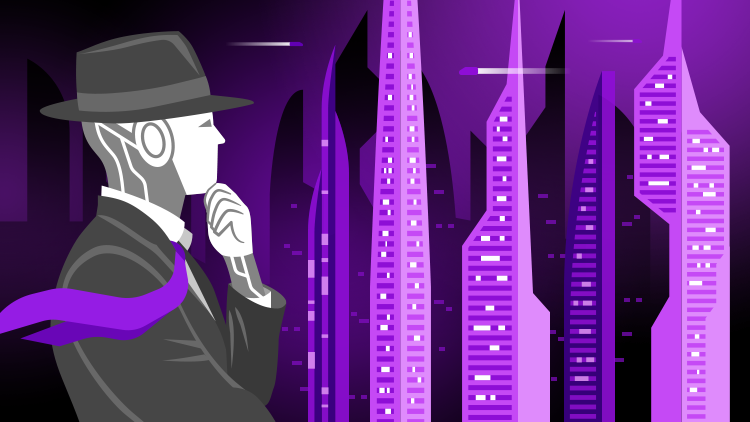
\includegraphics[scale=0.6]{Course_Image.png}
		\end{center}
\end{figure}

\end{titlepage}

{
\setcounter{tocdepth}{1}
\tableofcontents
}
\textbackslash{}begin\{titlepage\}

\setcounter{tocdepth}{4}
\renewcommand{\contentsname}{Tabla de Contenidos}
\tableofcontents

\newpage

\hypertarget{introducciuxf3n}{%
\chapter{Introducción}\label{introducciuxf3n}}

This book goes hand in hand with our ``Artificial Intelligence for Business'' e-course (\href{https://www.udemy.com/ai-for-business/?couponCode=THEBOOK}{link here}). It covers three Real World Business Case Studies, which we will solve with three different AI Solutions:

\begin{longtable}[]{@{}ccc@{}}
\toprule
\begin{minipage}[b]{0.19\columnwidth}\centering
\textbf{Part}\strut
\end{minipage} & \begin{minipage}[b]{0.34\columnwidth}\centering
\textbf{Case Study}\strut
\end{minipage} & \begin{minipage}[b]{0.38\columnwidth}\centering
\textbf{AI Solution}\strut
\end{minipage}\tabularnewline
\midrule
\endhead
\begin{minipage}[t]{0.19\columnwidth}\centering
1 - Optimizing Processes\strut
\end{minipage} & \begin{minipage}[t]{0.34\columnwidth}\centering
Optimizing the flows in an E-commerce warehouse\strut
\end{minipage} & \begin{minipage}[t]{0.38\columnwidth}\centering
Q-Learning\strut
\end{minipage}\tabularnewline
\begin{minipage}[t]{0.19\columnwidth}\centering
2 - Minimizing Costs\strut
\end{minipage} & \begin{minipage}[t]{0.34\columnwidth}\centering
Minimizing energy related costs of a data center\strut
\end{minipage} & \begin{minipage}[t]{0.38\columnwidth}\centering
Deep Q-Learning\strut
\end{minipage}\tabularnewline
\begin{minipage}[t]{0.19\columnwidth}\centering
3 - Maximizing Revenues\strut
\end{minipage} & \begin{minipage}[t]{0.34\columnwidth}\centering
Maximizing revenue of an online retail business\strut
\end{minipage} & \begin{minipage}[t]{0.38\columnwidth}\centering
Thompson Sampling\strut
\end{minipage}\tabularnewline
\bottomrule
\end{longtable}

In each of these parts we will always follow the same 3-steps process:

\begin{itemize}
\tightlist
\item
  \textbf{Case Study.} We will start by explaining the problem we have to solve and we will build from scratch the environment we will be working on.
\item
  \textbf{AI Solution.} We will give you not only the Intuition but also all the mathematical details of the AI model that will solve the case study.
\item
  \textbf{Implementation.} We will implement the whole AI Solution in Python, go into production, and improve the AI by completing two Homeworks.
\end{itemize}

Thank you all so much for joining us, we wish you an exciting journey into the world of AI for Business!

\hypertarget{part-1---optimizing-processes}{%
\chapter{Part 1 - Optimizing Processes}\label{part-1---optimizing-processes}}

Here we go with our first case study and our first AI model. We hope you are ready.

\hypertarget{case-study-optimizing-the-flows-in-an-e-commerce-warehouse}{%
\section{Case Study: Optimizing the Flows in an E-Commerce Warehouse}\label{case-study-optimizing-the-flows-in-an-e-commerce-warehouse}}

\hypertarget{problem-to-solve}{%
\subsection{Problem to solve}\label{problem-to-solve}}

The problem to solve will be to optimize the flows inside the following warehouse:

\begin{figure}[!htbp]
        \begin{center}
            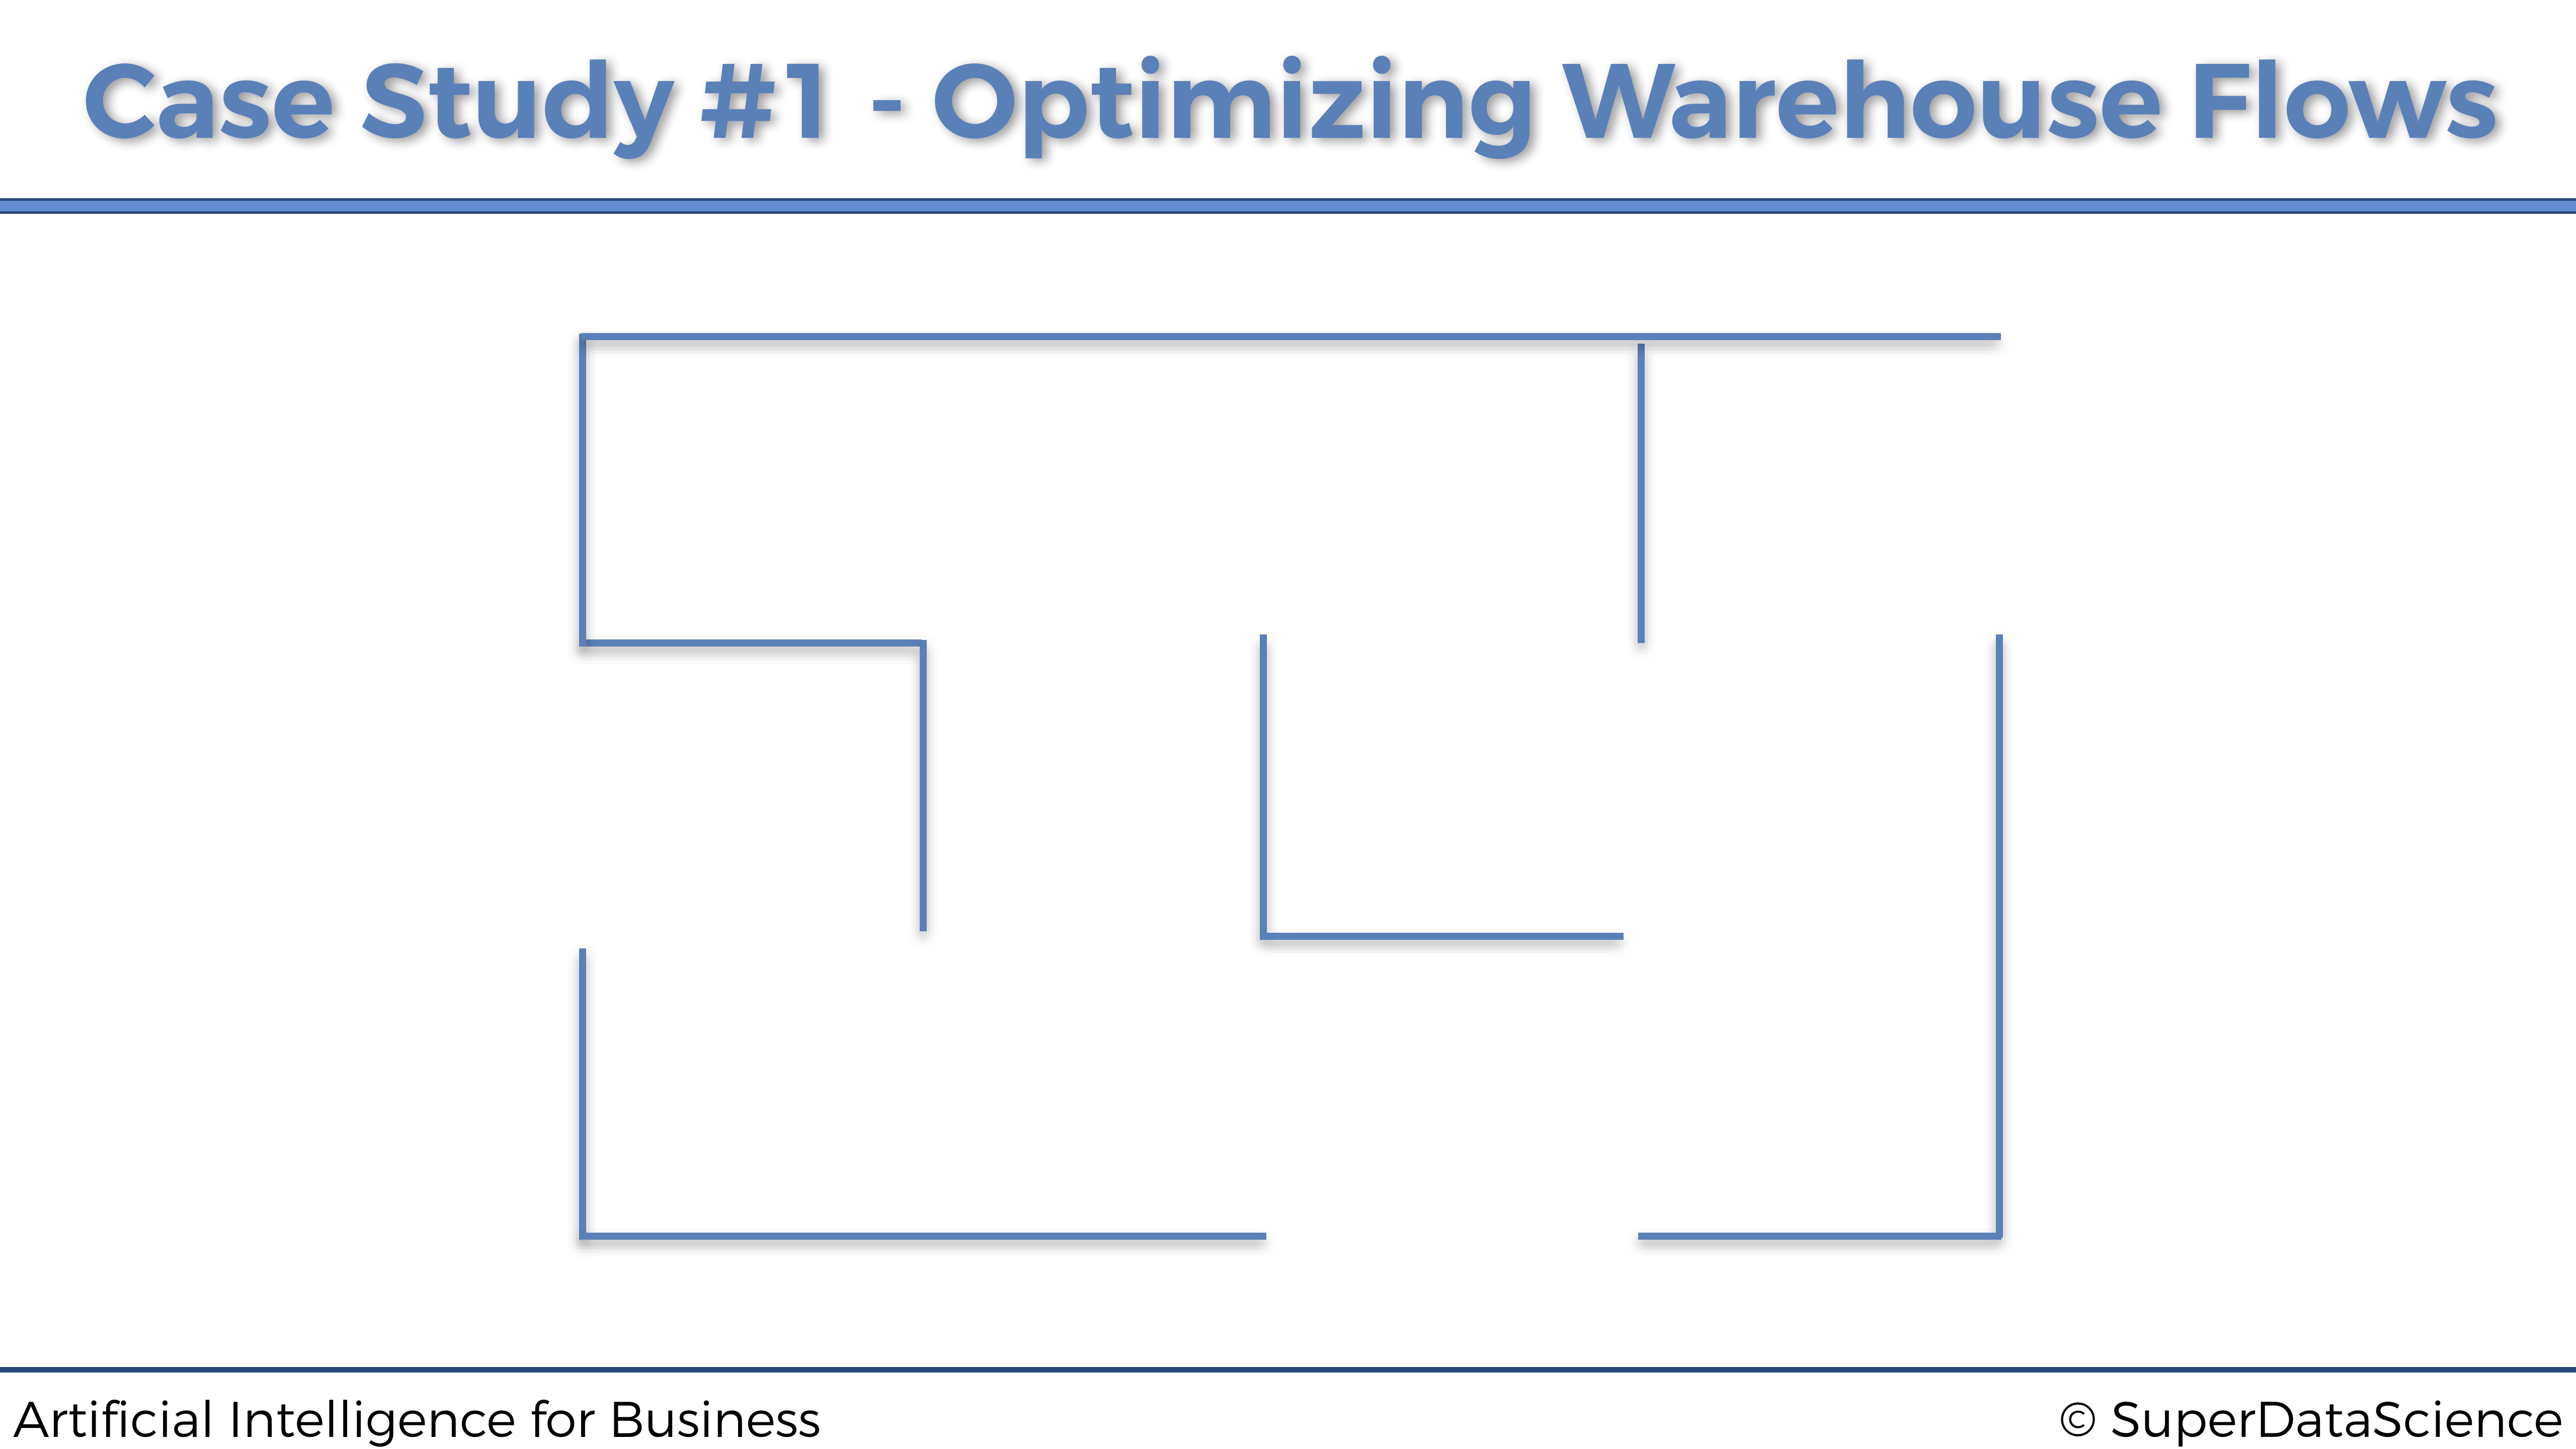
\includegraphics[scale=0.15]{Warehouse_1.png}
        \end{center}
\end{figure}

The warehouse belongs to an online retail company that sells products to a variety of customers. Inside this warehouse, the products are stored in 12 different locations, labeled by the following letters from A to L:

\begin{figure}[!htbp]
        \begin{center}
            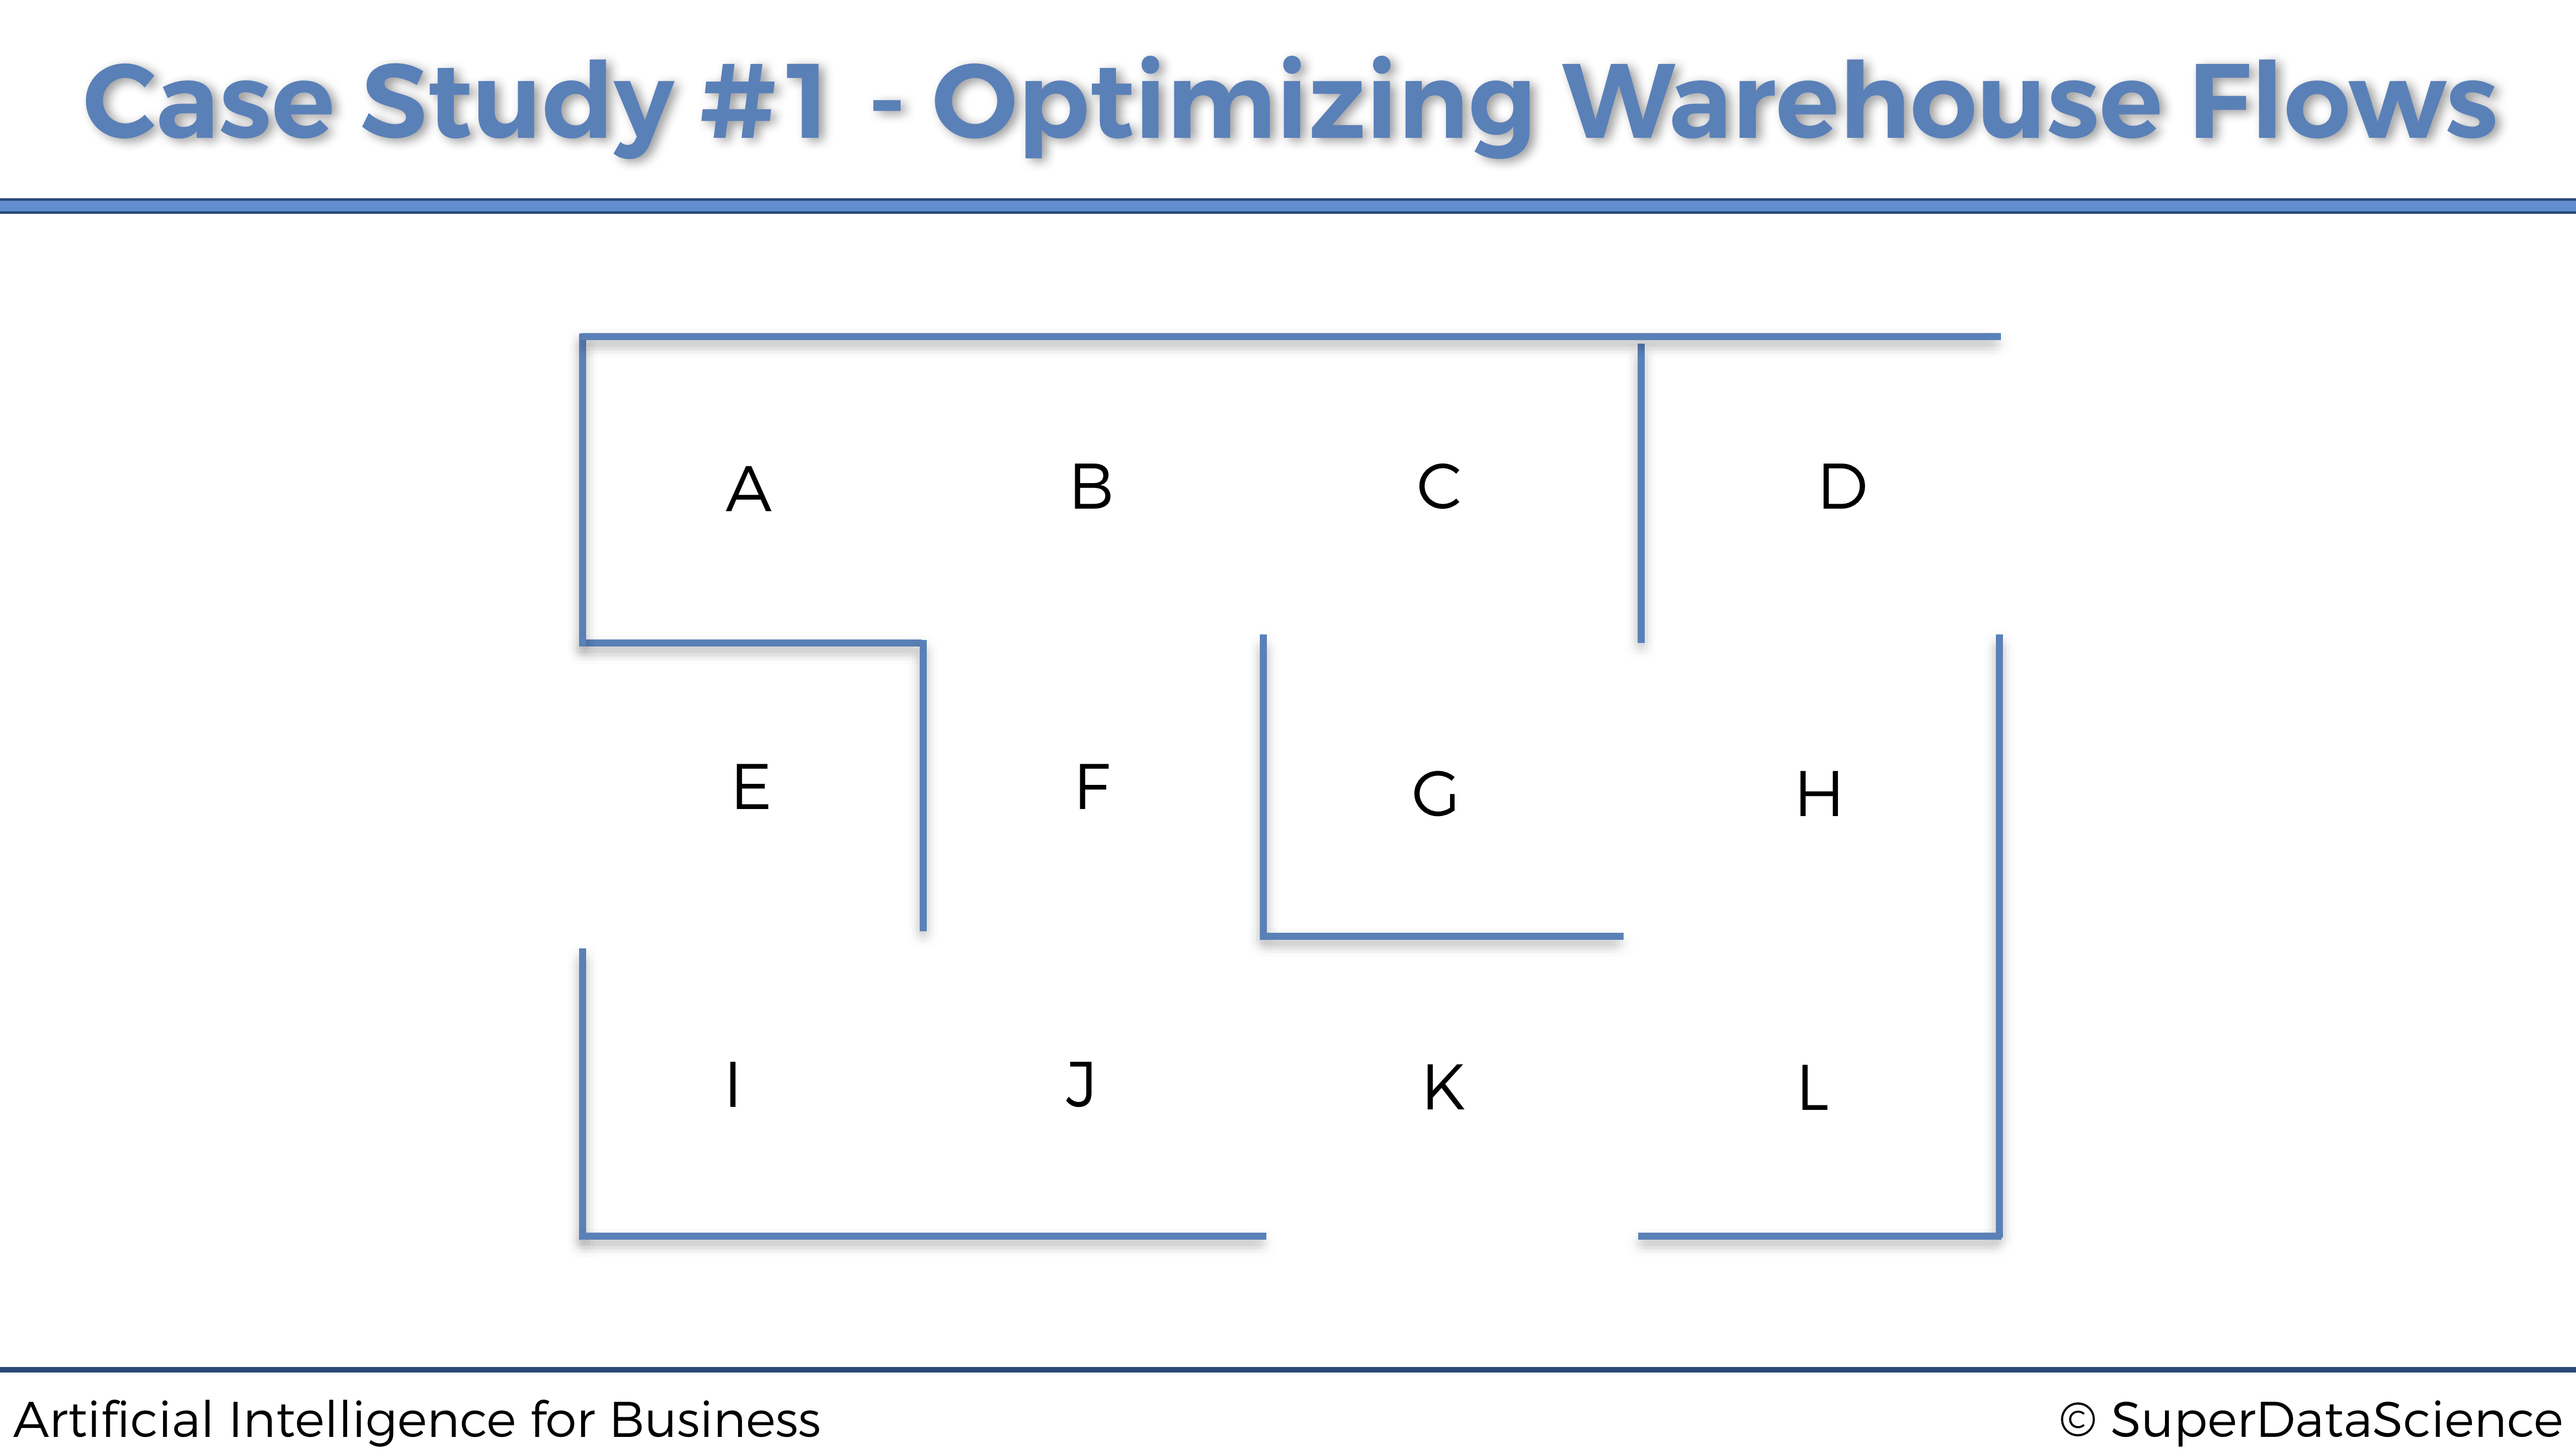
\includegraphics[scale=0.15]{Warehouse_2.png}
        \end{center}
\end{figure}

As the orders are placed by the customers online, an Autonomous Warehouse Robot is moving around the warehouse to collect the products for future deliveries. Here is what it looks like:

\begin{figure}[!htbp]
        \begin{center}
            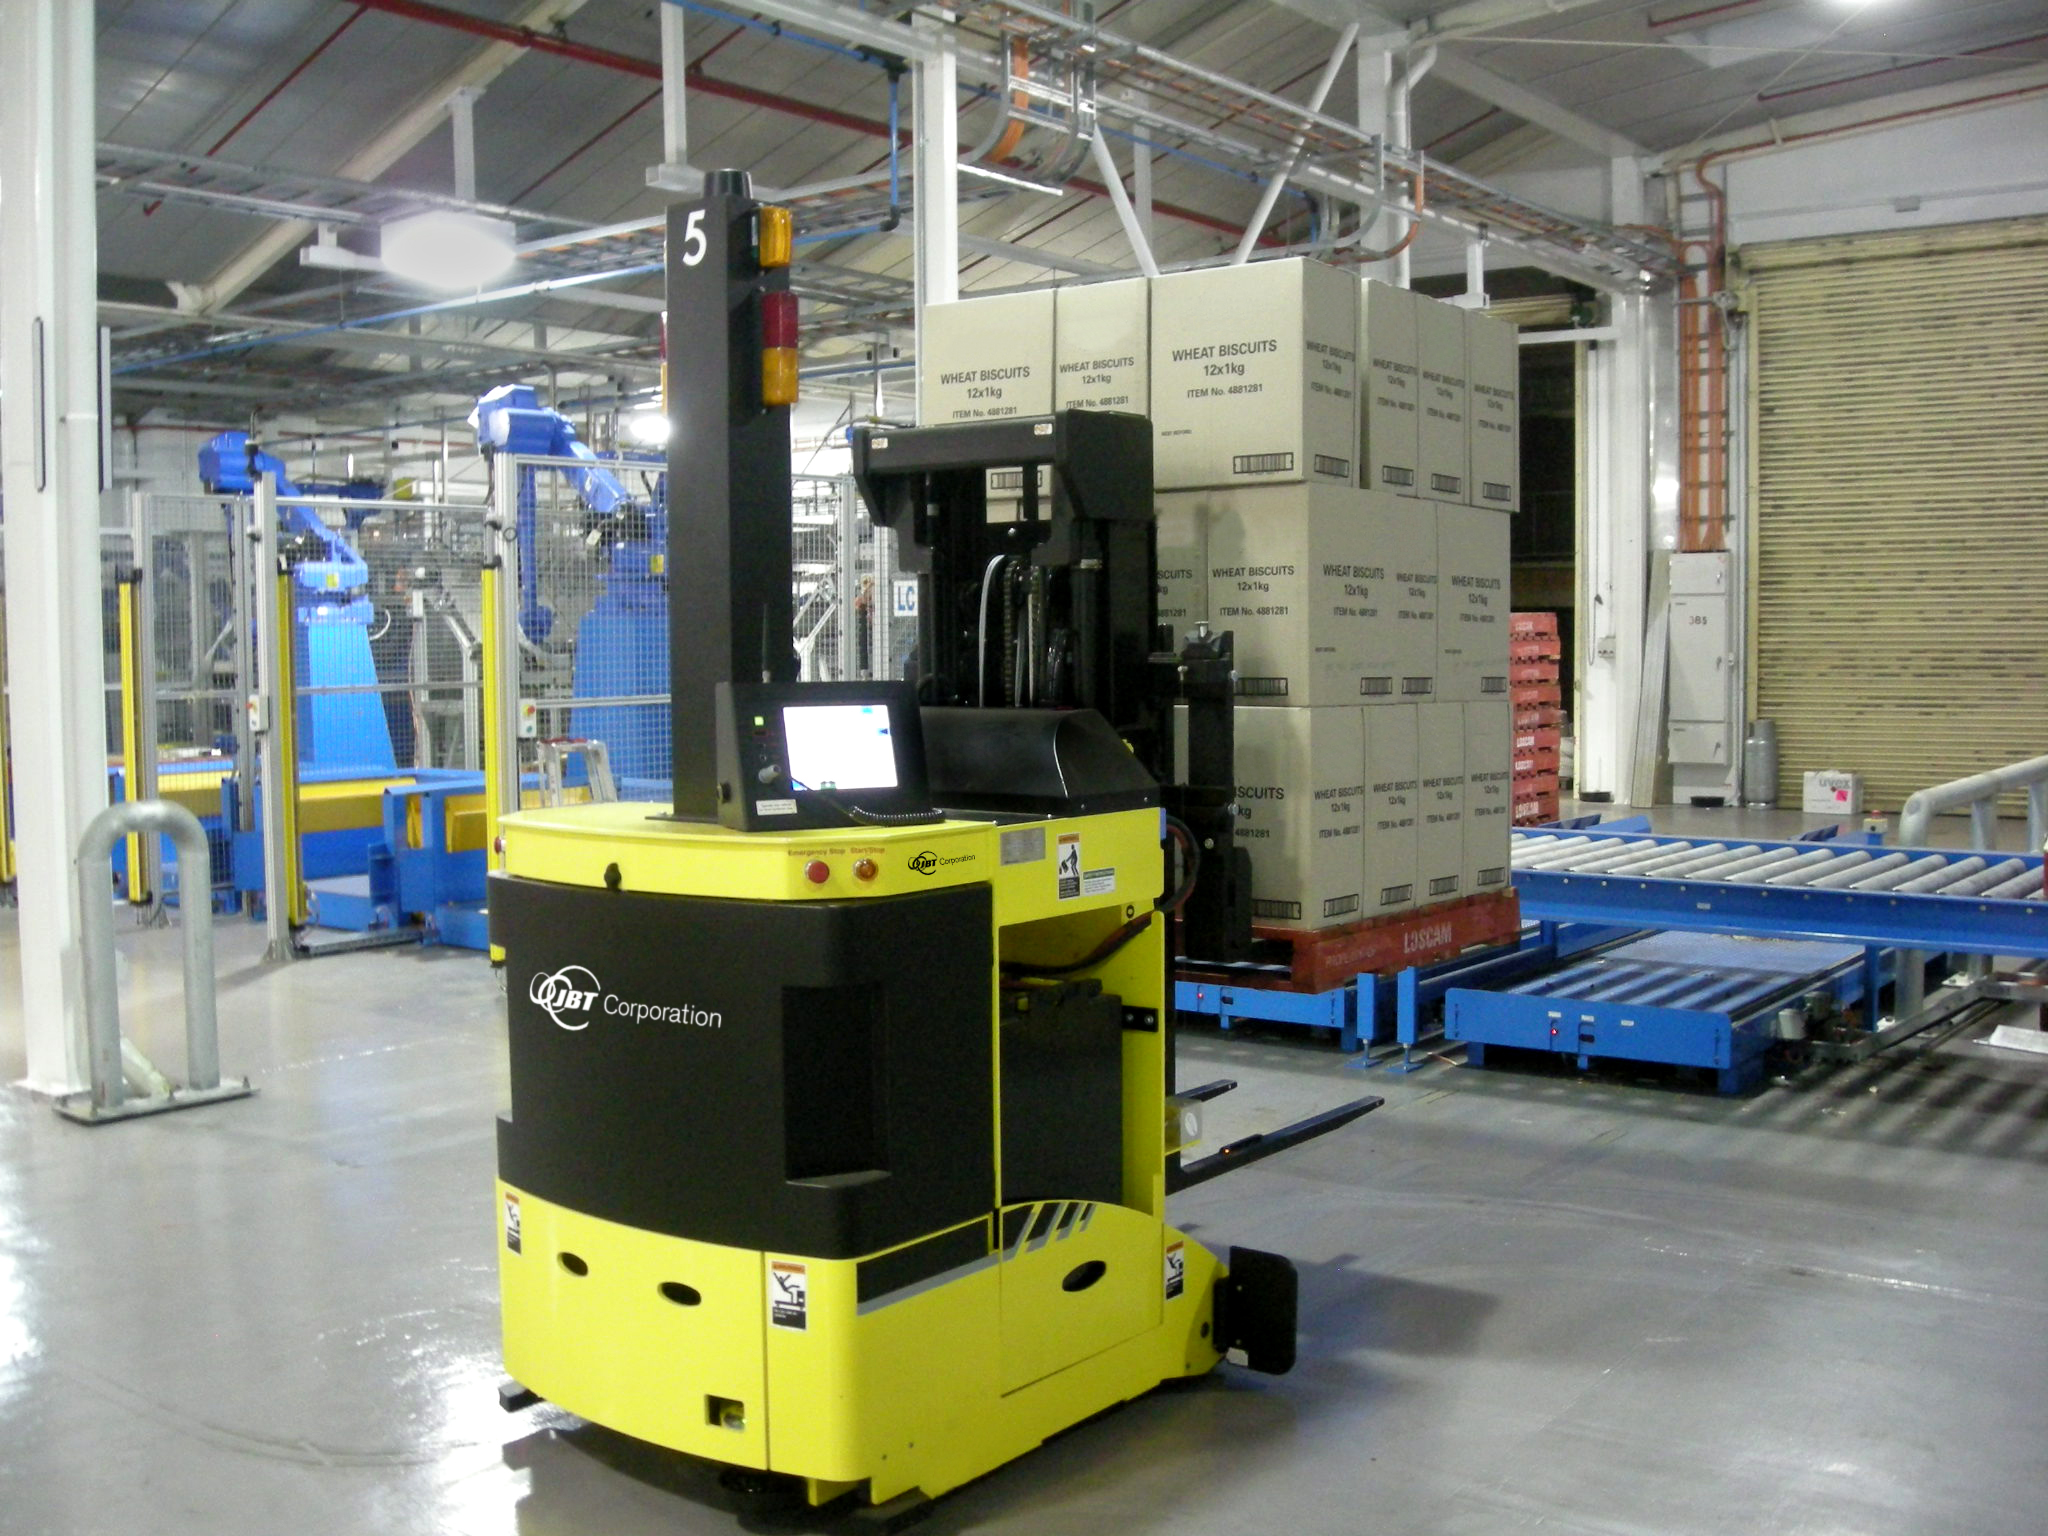
\includegraphics[scale=0.75]{Autonomous_Warehouse_Robot.jpg}
            \caption{Autonomous Warehouse Robot}
        \end{center}
\end{figure}

The 12 locations are all connected to a computer system, which is ranking in real time the priorities of product collection for these 12 locations. For example, at a specific time \(t\), it will return the following ranking:

\begin{table}[h!]
  \begin{center}
    \begin{tabular}{c|c}
      \textbf{Priority Rank} & \textbf{Location} \\
      \hline
      1 & G \\
      2 & K \\
      3 & L \\
      4 & J \\
      5 & A \\
      6 & I \\
      7 & H \\
      8 & C \\
      9 & B \\
      10 & D \\
      11 & F \\
      12 & E \\
    \end{tabular}
  \end{center}
\end{table}

Location G has priority 1, which means it is the top priority, as it contains a product that must be collected and delivered immediately. Our Autonomous Warehouse Robot must move to location G by the shortest route depending on where it is. Our goal is to build an AI that will return that shortest route, wherever the robot is. But then as we see, locations K and L are in the Top 3 priorities. Hence we will want to implement an option for our Autonomous Warehouse Robot to go by some intermediary locations before reaching its final top priority location.

The way the system computes the priorities of the locations is out of the scope of this case study. The reason for this is that there can be many ways, from simple rules or algorithms, to deterministic computations, to machine learning. But most of these ways would not be artificial intelligence as we know it today. What we really want to focus on is core AI, encompassing Q-Learning, Deep Q-Learning and other branches of Reinforcement Learning. So we will just say for example that Location G is top priority because one of the most loyal platinum customers of the company placed an urgent order of a product stored in location G which therefore must be delivered as soon as possible.

Therefore in conclusion, our mission is to build an AI that will always take the shortest route to the top priority location, whatever the location it starts from, and having the option to go by an intermediary location which is in the top 3 priorities.

\subsubsection{Environment to define}

When building an AI, the first thing we always have to do is to define the environment. And defining an environment always requires the three following elements:

\begin{itemize}
    \item Defining the states
    \item Defining the actions
    \item Defining the rewards
\end{itemize}

Let's define these three elements, one by one.

\textbf{Defining the states.}

Let's start with the states. The input state is simply the location where our Autonomous Warehouse Robot is at each time \(t\). However since we will build our AI with mathematical equations, we will encode the locations names (A, B, C,\ldots{}) into index numbers, with respect to the following mapping:

\begin{table}[h!]
  \begin{center}
    \begin{tabular}{c|c}
      \textbf{Location} & \textbf{State} \\
      \hline
      A & 0 \\
      B & 1 \\
      C & 2 \\
      D & 3 \\
      E & 4 \\
      F & 5 \\
      G & 6 \\
      H & 7 \\
      I & 8 \\
      J & 9 \\
      K & 10 \\
      L & 11 \\
    \end{tabular}
  \end{center}
\end{table}

There is a specific reason why we encode the states with indexes from 0 to 11, instead of other integers. The reason is that we will work with matrices, a matrix of rewards and a matrix of Q-Values, and each line/column of these matrices will correspond to a specific location. For example, the first line of each matrix, which has index 0, corresponds to location A. The second line/column, which has index 1, corresponds to location B. Etc. We will see the purpose of working with matrices in more details a bit later.

\textbf{Defining the actions.}

Now let's define the possible actions to play. The actions are simply the next moves the robot can make to go from one location to the next. So for example, let's say the robot is in location J, the possible actions that the robot can play is to go to I, to F, or to K. And again, since we will work with mathematical equations, we will encode these actions with the same indexes as for the states. Hence, following our same example where the robot is in location J at a specific time, the possible actions that the robot can play are, according to our previous mapping above: 5, 8 and 10. Indeed, the index 5 corresponds to F, the index 8 corresponds to I, and the index 10 corresponds to K. Therefore eventually, the total list of actions that the AI can play overall is the following:

\begin{lstlisting}
actions = [0,1,2,3,4,5,6,7,8,9,10,11]
\end{lstlisting}

Obviously, when being in a specific location, there are some actions that the robot cannot play. Taking the same previous example, if the robot is in location J, it can play the actions 5, 8 and 10, but it cannot play the other actions. We will make sure to specify that by attributing a 0 reward to the actions it cannot play, and a 1 reward to the actions it can play. And that brings us to the rewards.

\textbf{Defining the rewards.}

The last thing that we have to do now to build our environment is to define a system of rewards. More specifically, we have to define a reward function R that takes as inputs a state \(s\) and an action \(a\), and returns a numerical reward that the AI will get by playing the action \(a\) in the state \(s\):

\begin{equation*}
R : (\textrm{state}, \textrm{action}) \mapsto r \in \mathbb{R}
\end{equation*}

So how are we going to build such a function for our case study? Here this is simple. Since there is a discrete and finite number of states (the indexes from 0 to 11), as well as a discrete and finite number of actions (same indexes from 0 to 11), the best way to build our reward function R is to simply make a matrix. Our reward function will exactly be a matrix of 12 rows and 12 columns, where the rows correspond to the states, and the columns correspond to the actions. That way, in our function ``\(R : (s,a) \mapsto r \in \mathbb{R}\)'', \(s\) will be the row index of the matrix, \(a\) will be the column index of the matrix, and \(r\) will be the cell of indexes \((s,a)\) in the matrix.

Therefore the only thing that we have to do now to define our reward function is simply to populate this matrix with the numerical rewards. And as we just said in the previous paragraph, what we have to do first is to attribute, for each of the 12 locations, a 0 reward to the actions that the robot cannot play, and a 1 reward to the actions the robot can play. By doing that for each of the 12 locations, we will end up with a matrix of rewards. Let's build it step by step, starting with the first location: location A.

When being in location A, the robot can only go to location B. Therefore, since location A has index 0 (first row of the matrix) and location B has index 1 (second column of the matrix), the first row of the matrix of rewards will get a 1 on the second column, and a 0 on all the other columns, just like so:

\begin{figure}[!htbp]
        \begin{center}
            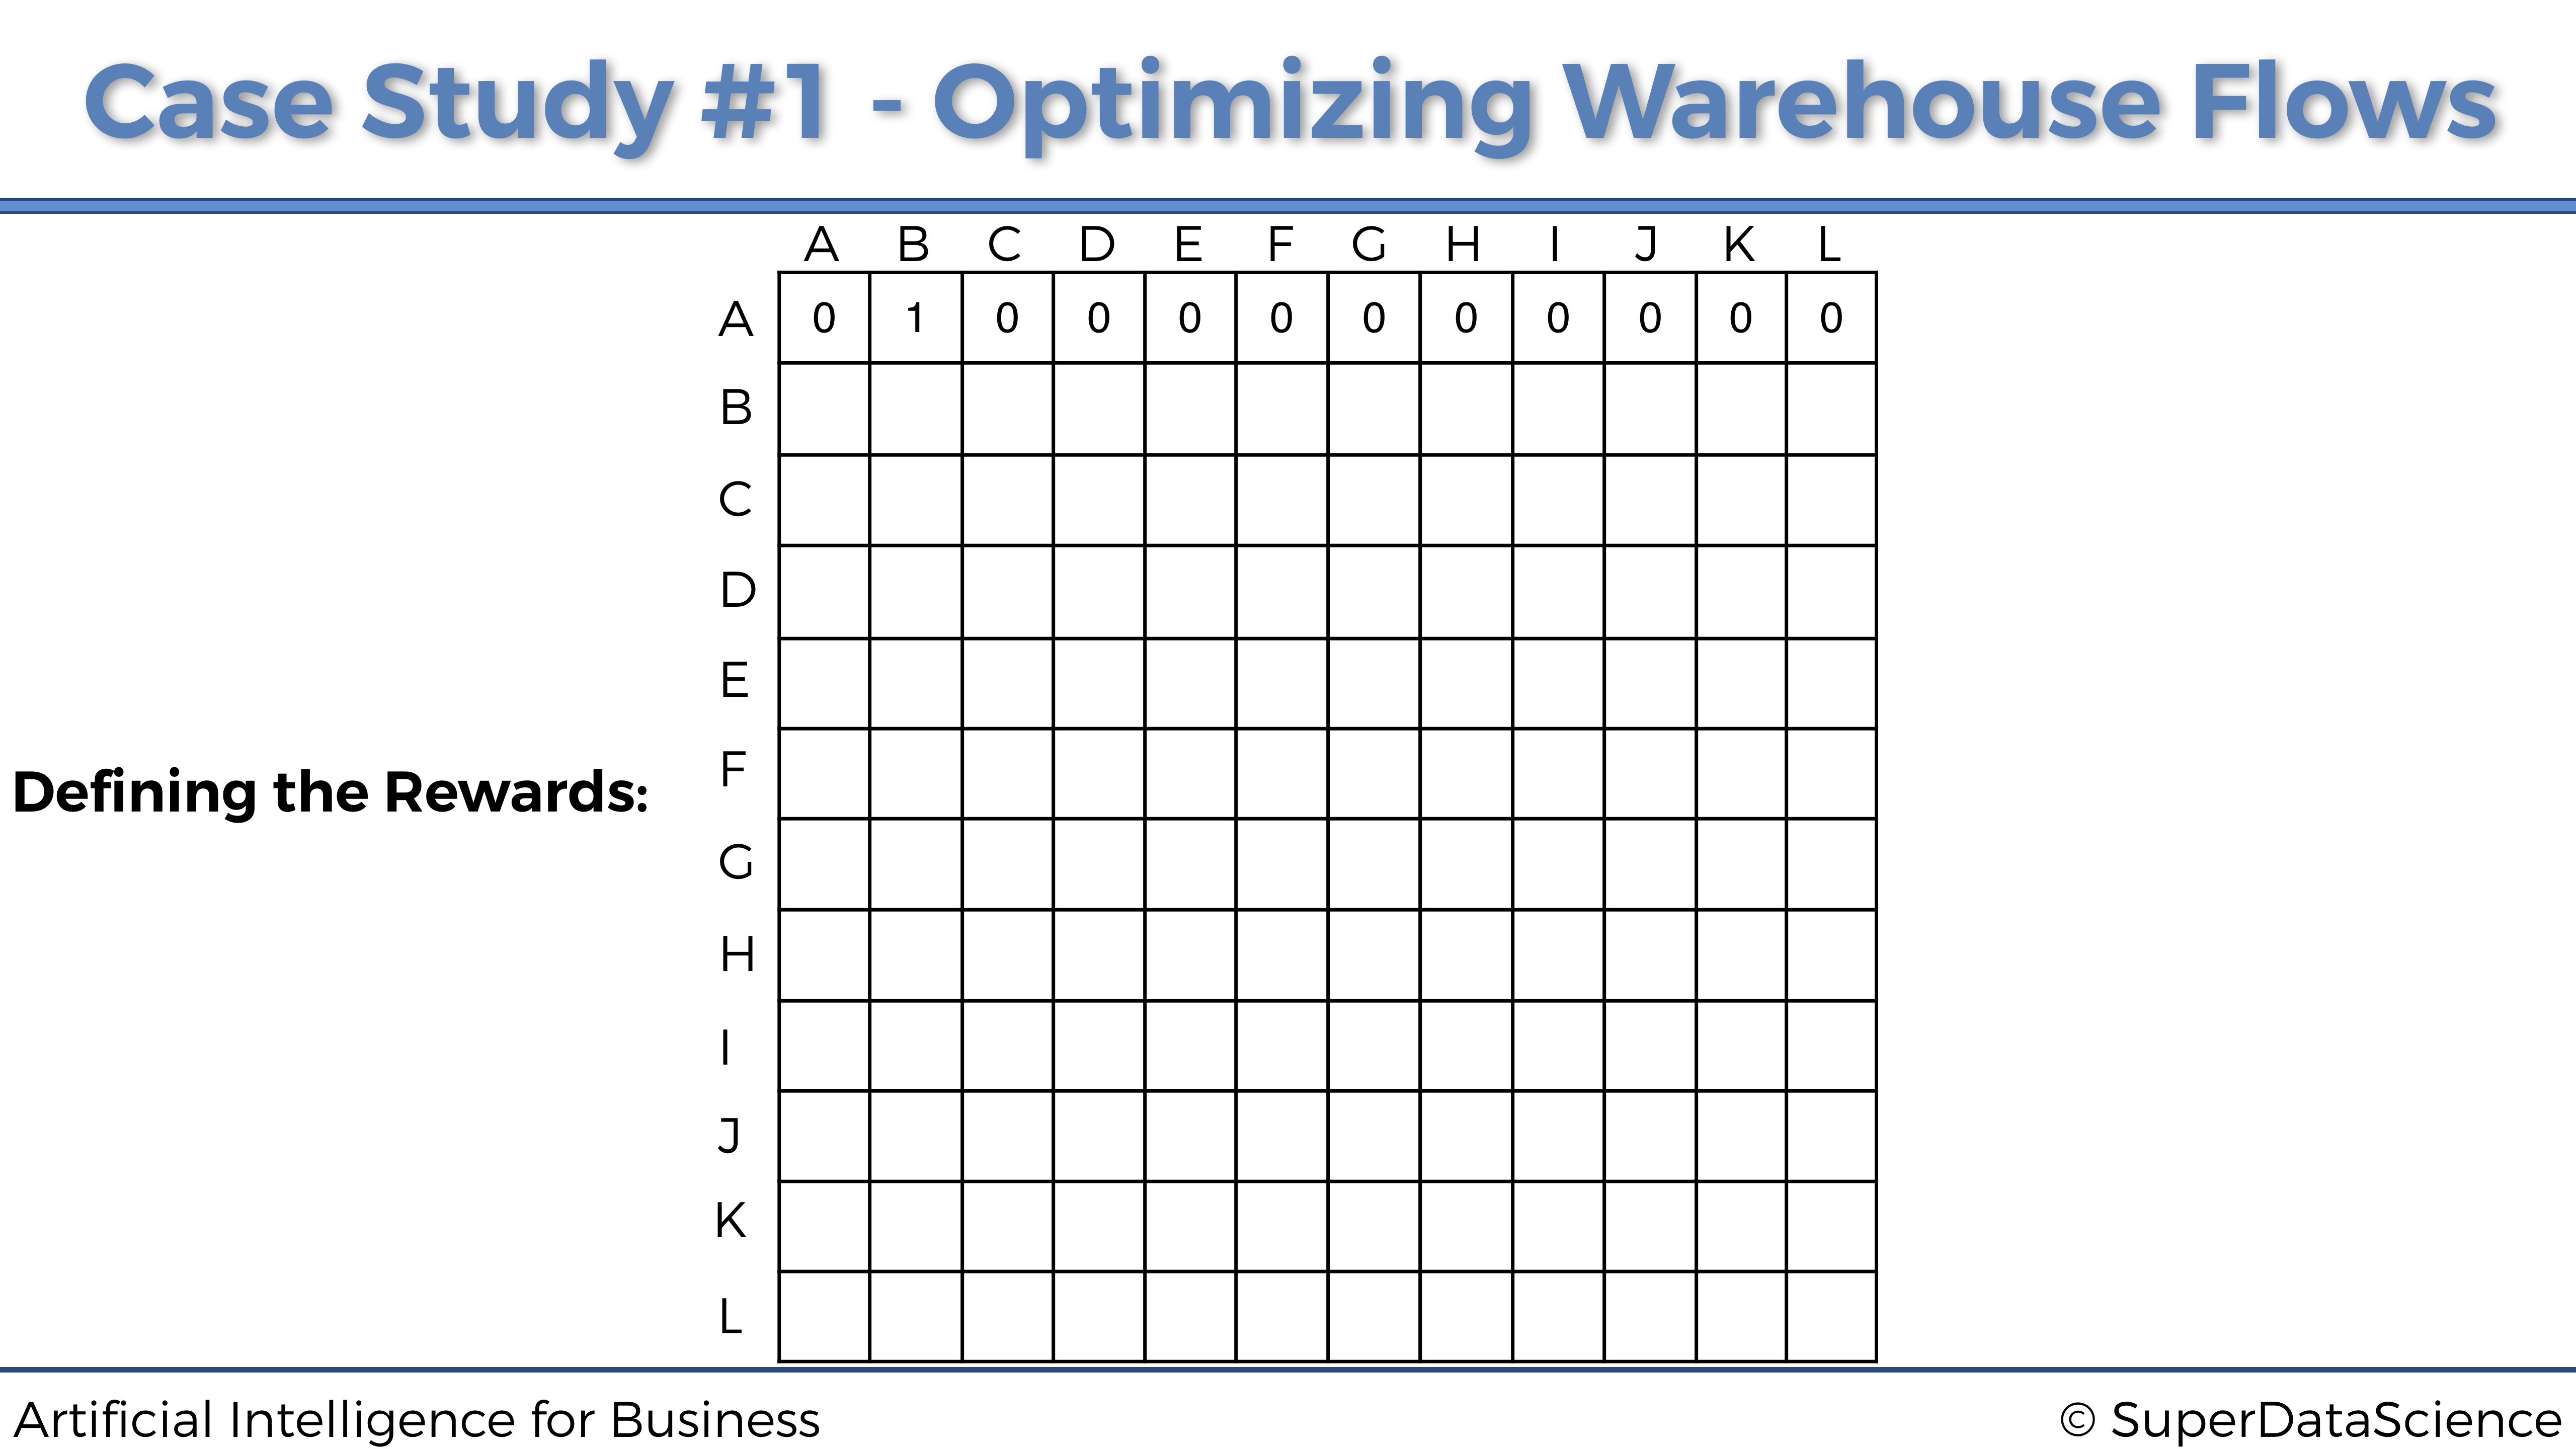
\includegraphics[scale=0.175]{Rewards_Matrix_1.png}
        \end{center}
\end{figure}

\newpage

Now let's move on to location B. When being in location B, the robot can only go to three different locations: A, C and F. Since B has index 1 (second row), and A, C, F have respective indexes 0, 2, 5 (1st, 3rd, and 6th column), then the second row of the matrix of rewards will get a 1 on the 1st, 3rd and 6th columns, and 0 on all the other columns. Hence we get:

\begin{figure}[!htbp]
        \begin{center}
            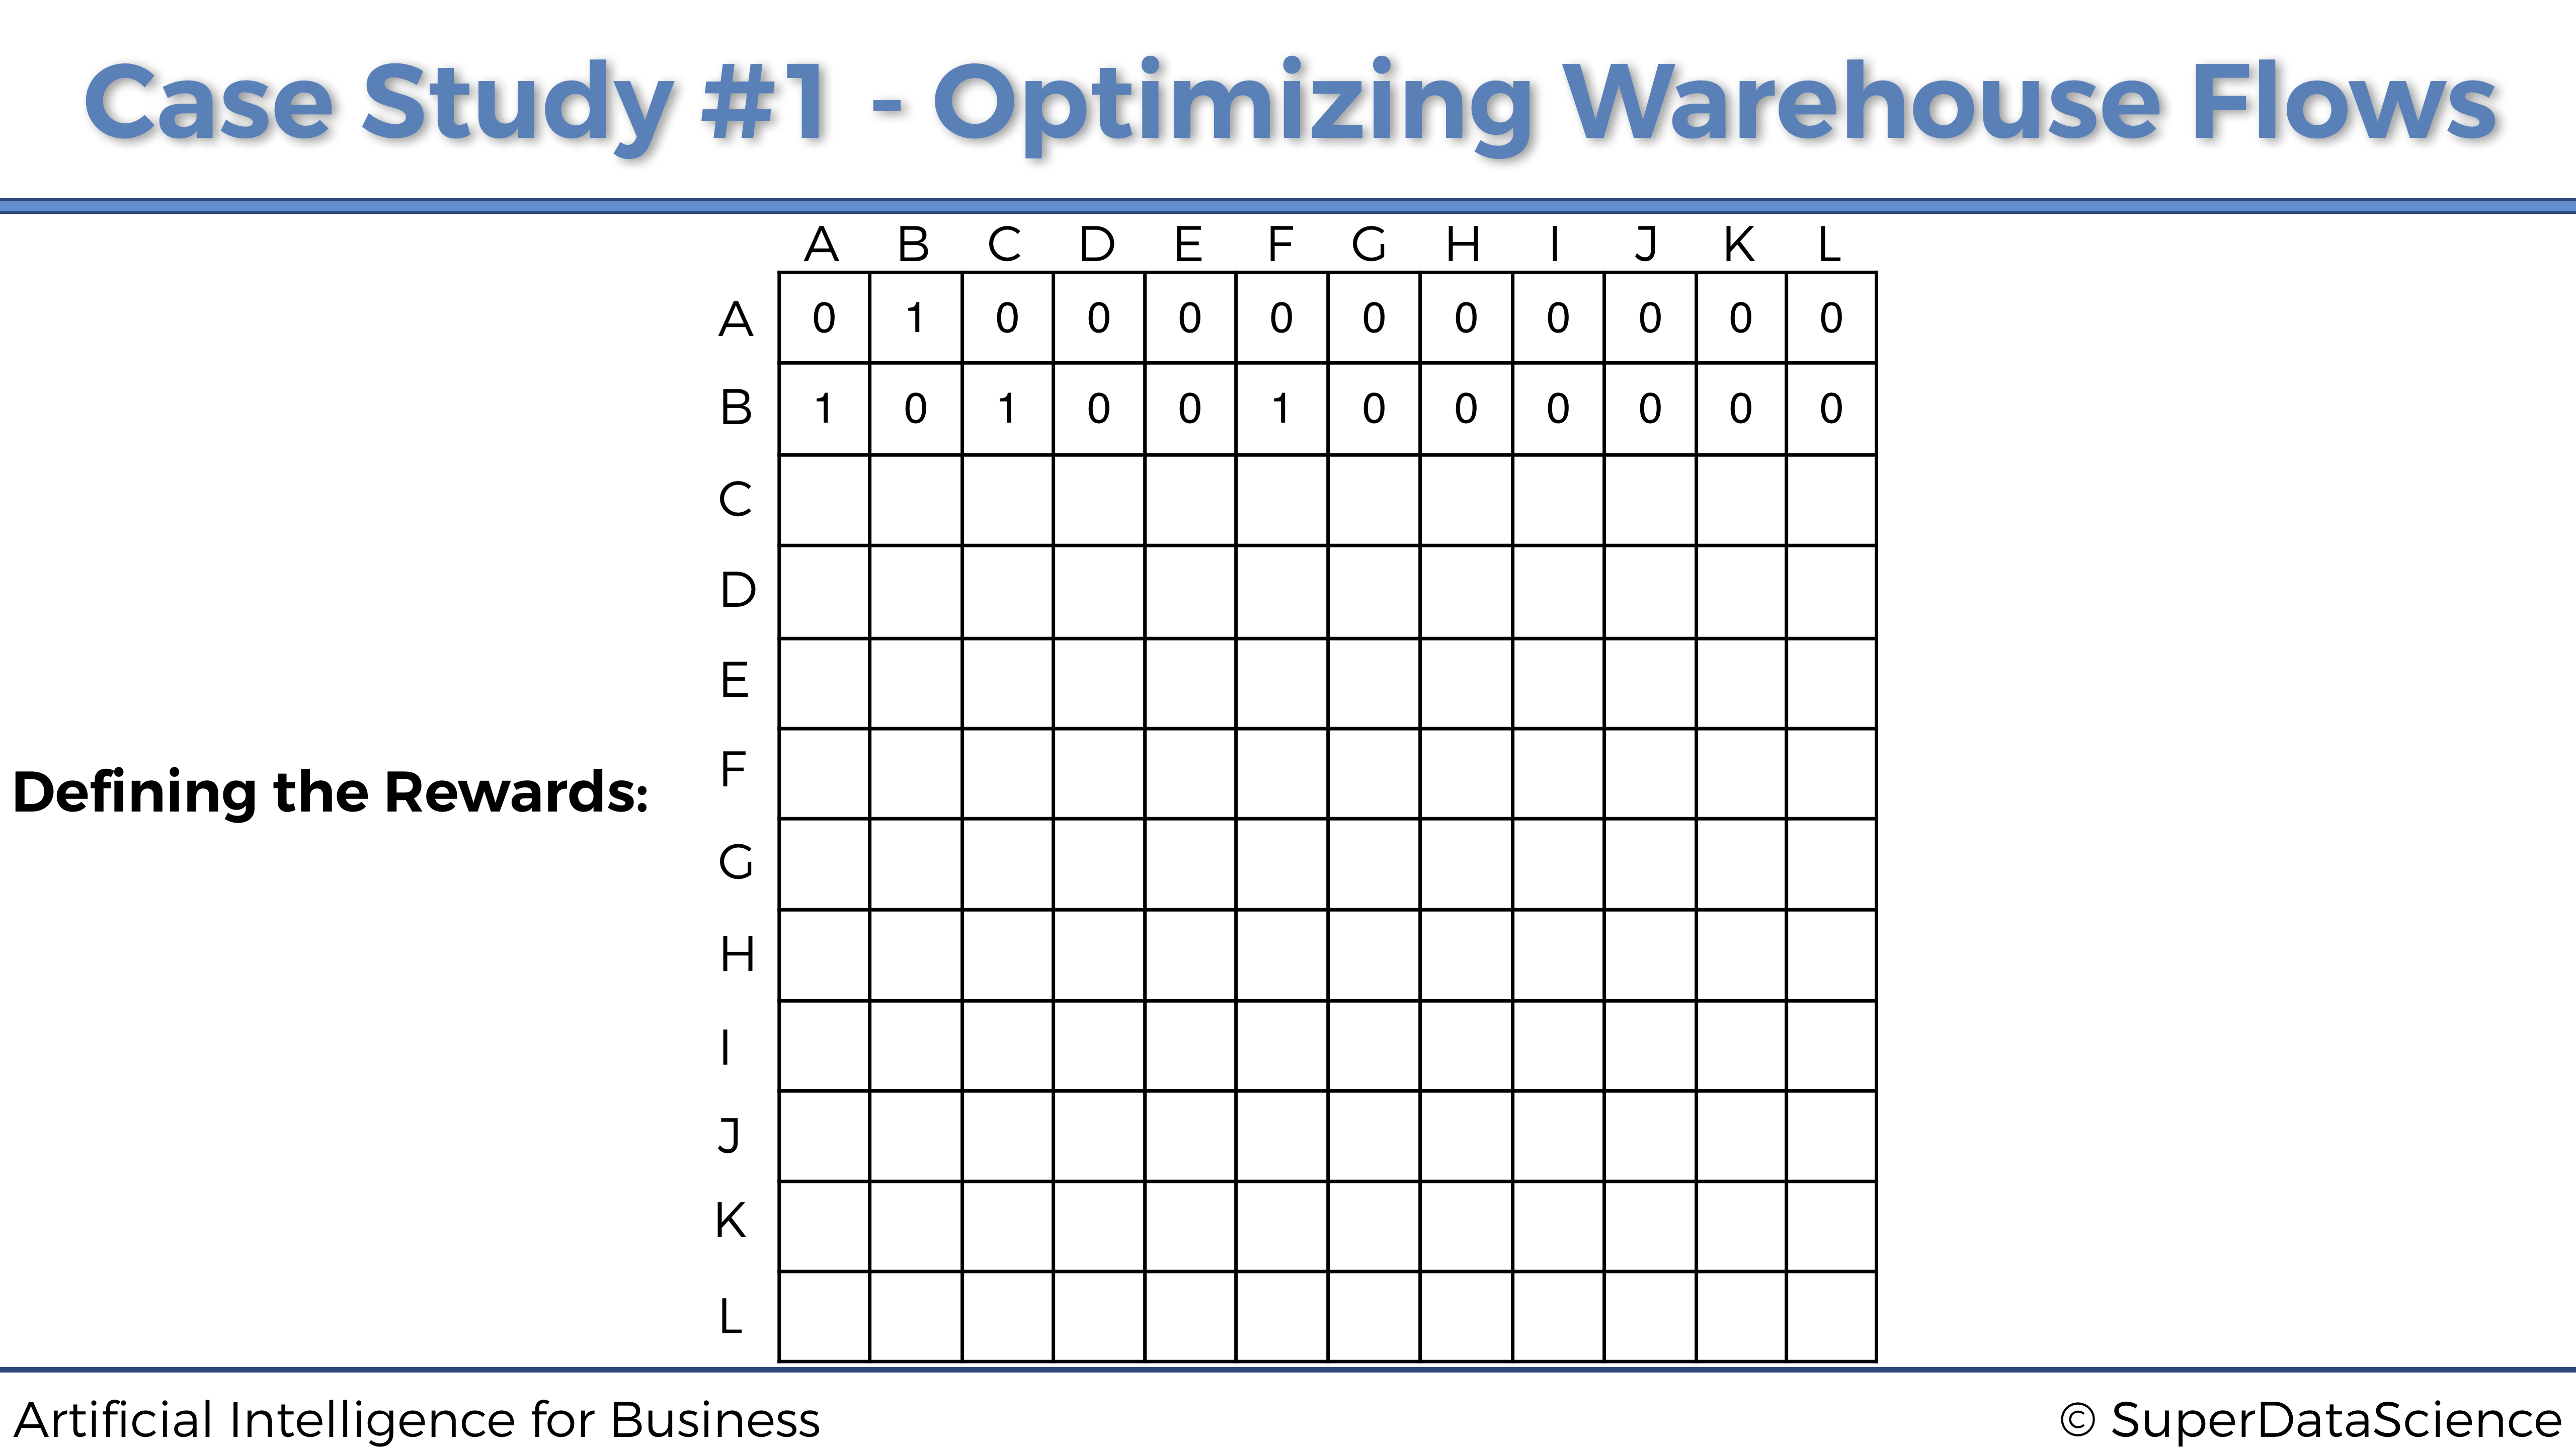
\includegraphics[scale=0.175]{Rewards_Matrix_2.png}
        \end{center}
\end{figure}

Then same, C (of index 2) is only connected to B and G (of indexes 1 and 6) so the third row of the matrix of rewards is:

\begin{figure}[!htbp]
        \begin{center}
            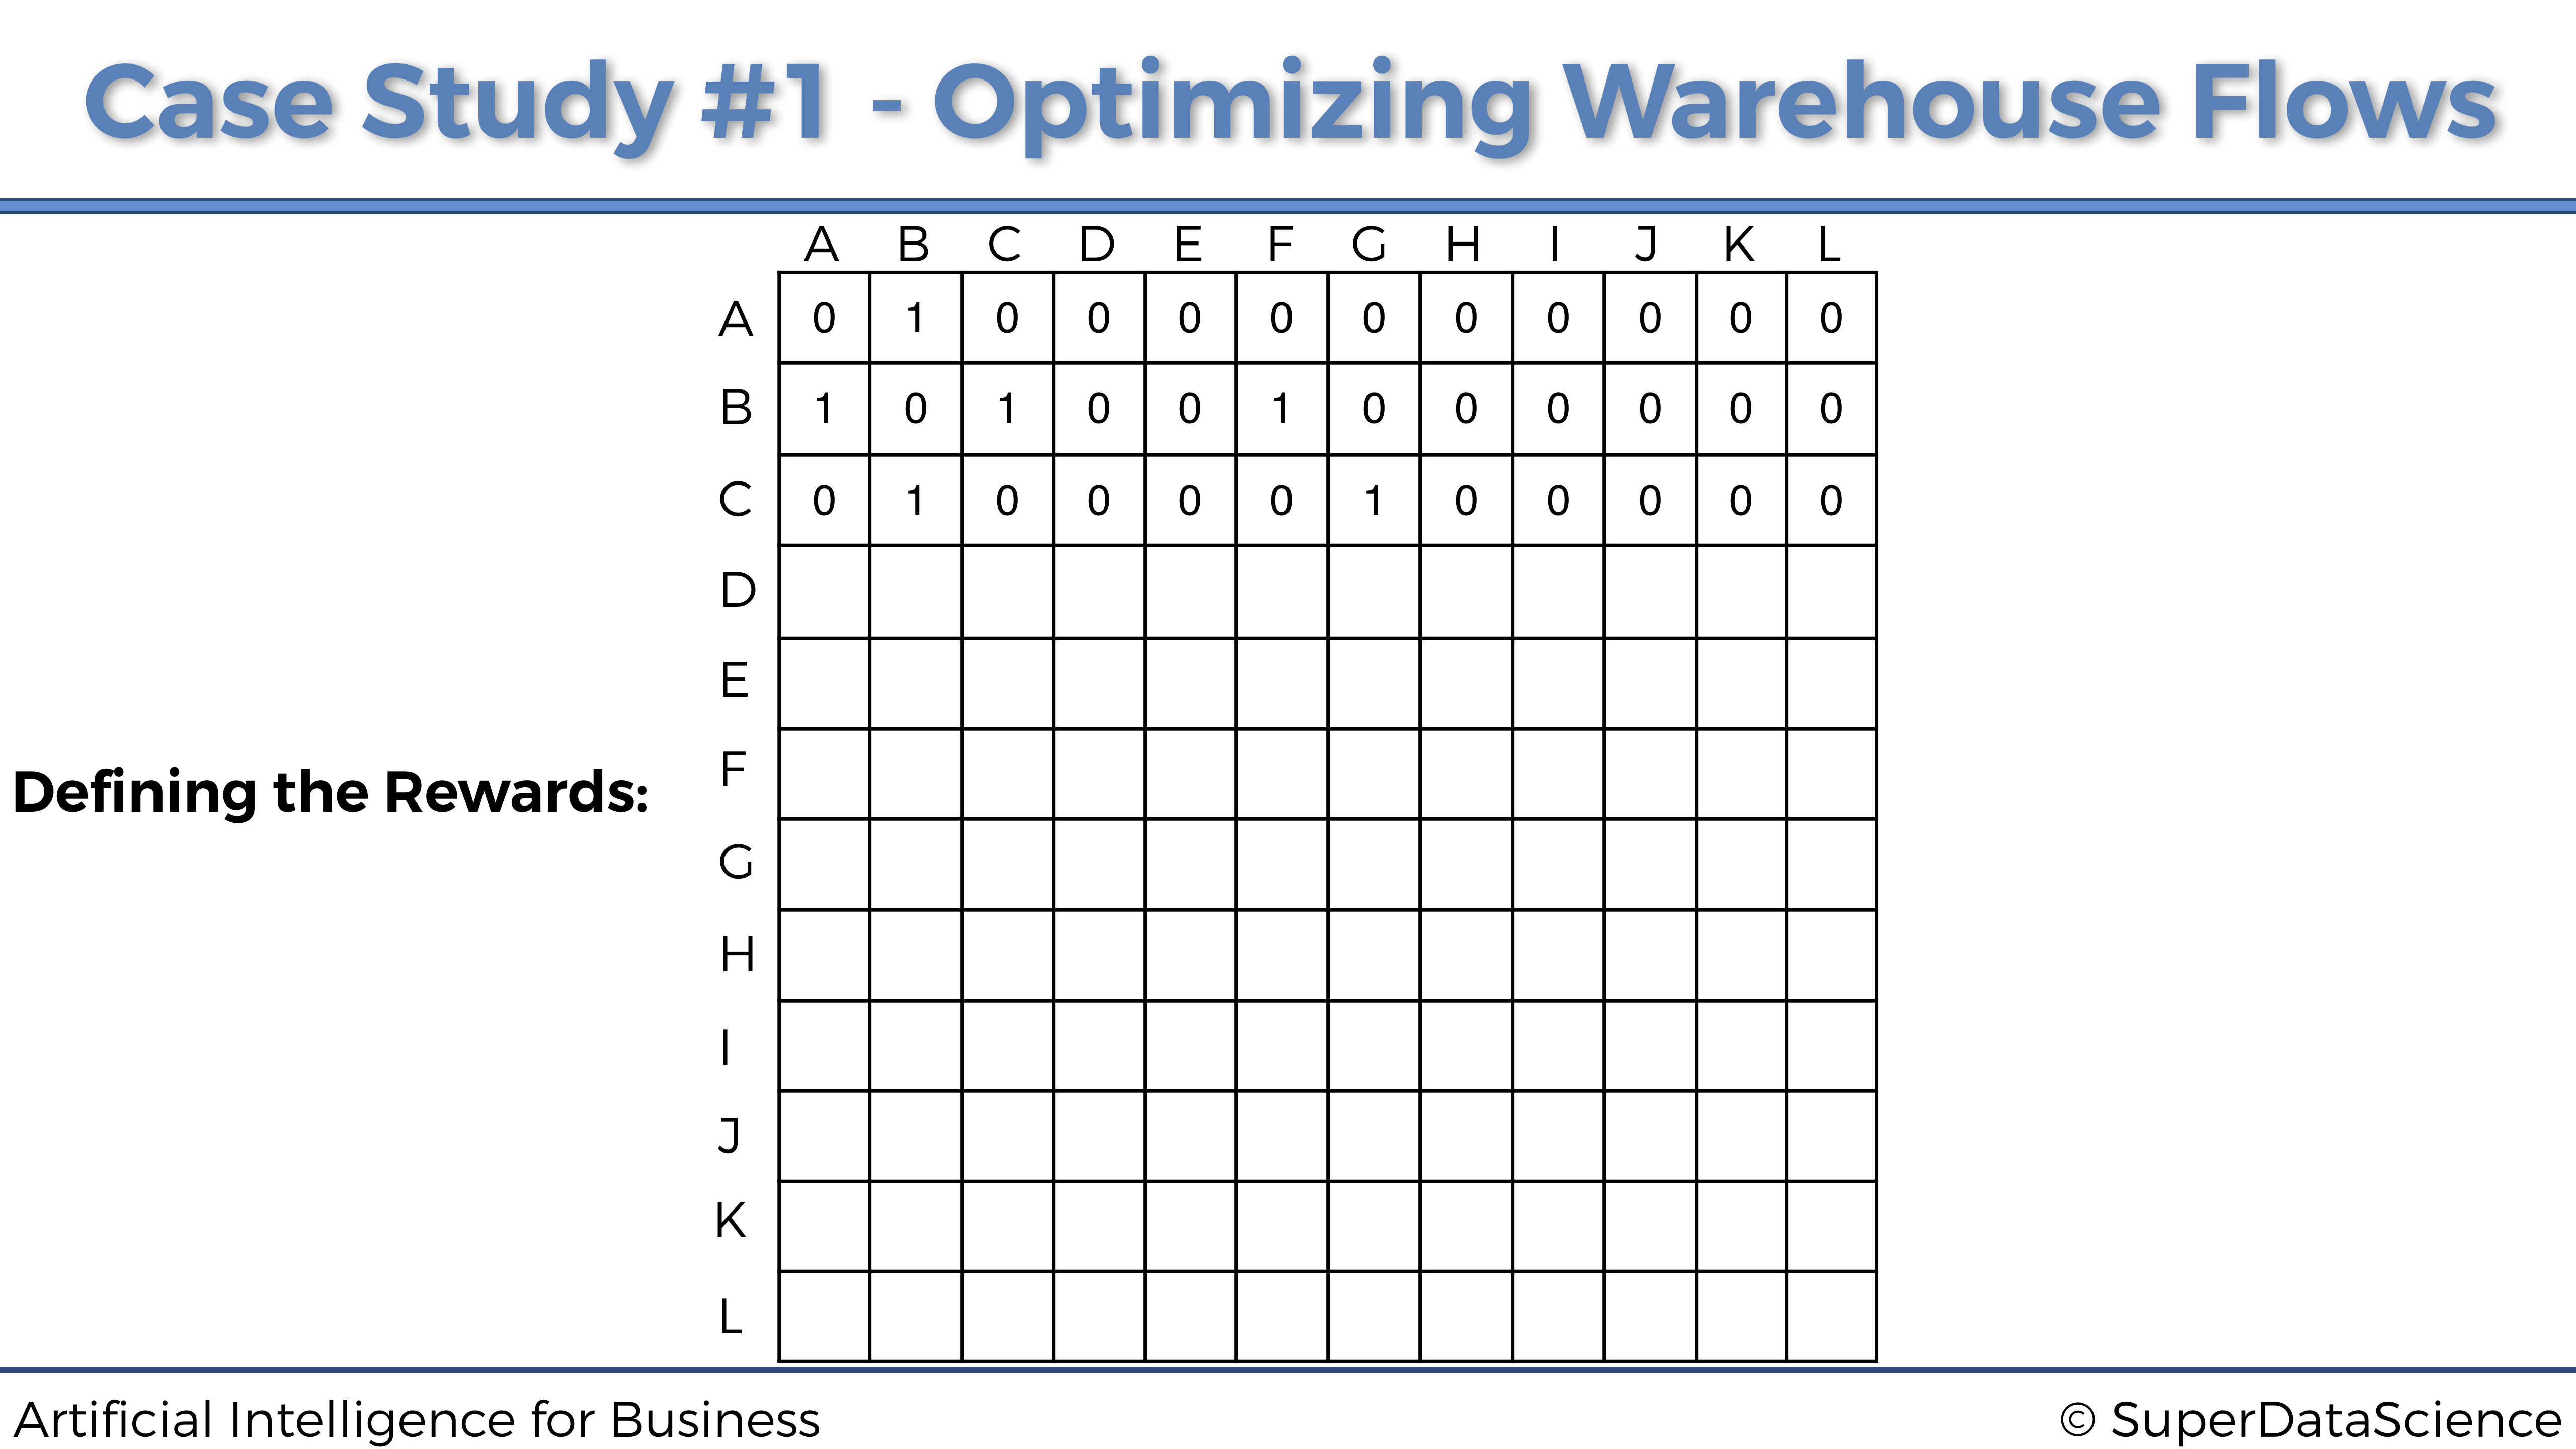
\includegraphics[scale=0.175]{Rewards_Matrix_3.png}
        \end{center}
\end{figure}

By doing the same for all the other locations, we eventually get our final matrix of rewards:

\begin{figure}[!htbp]
        \begin{center}
            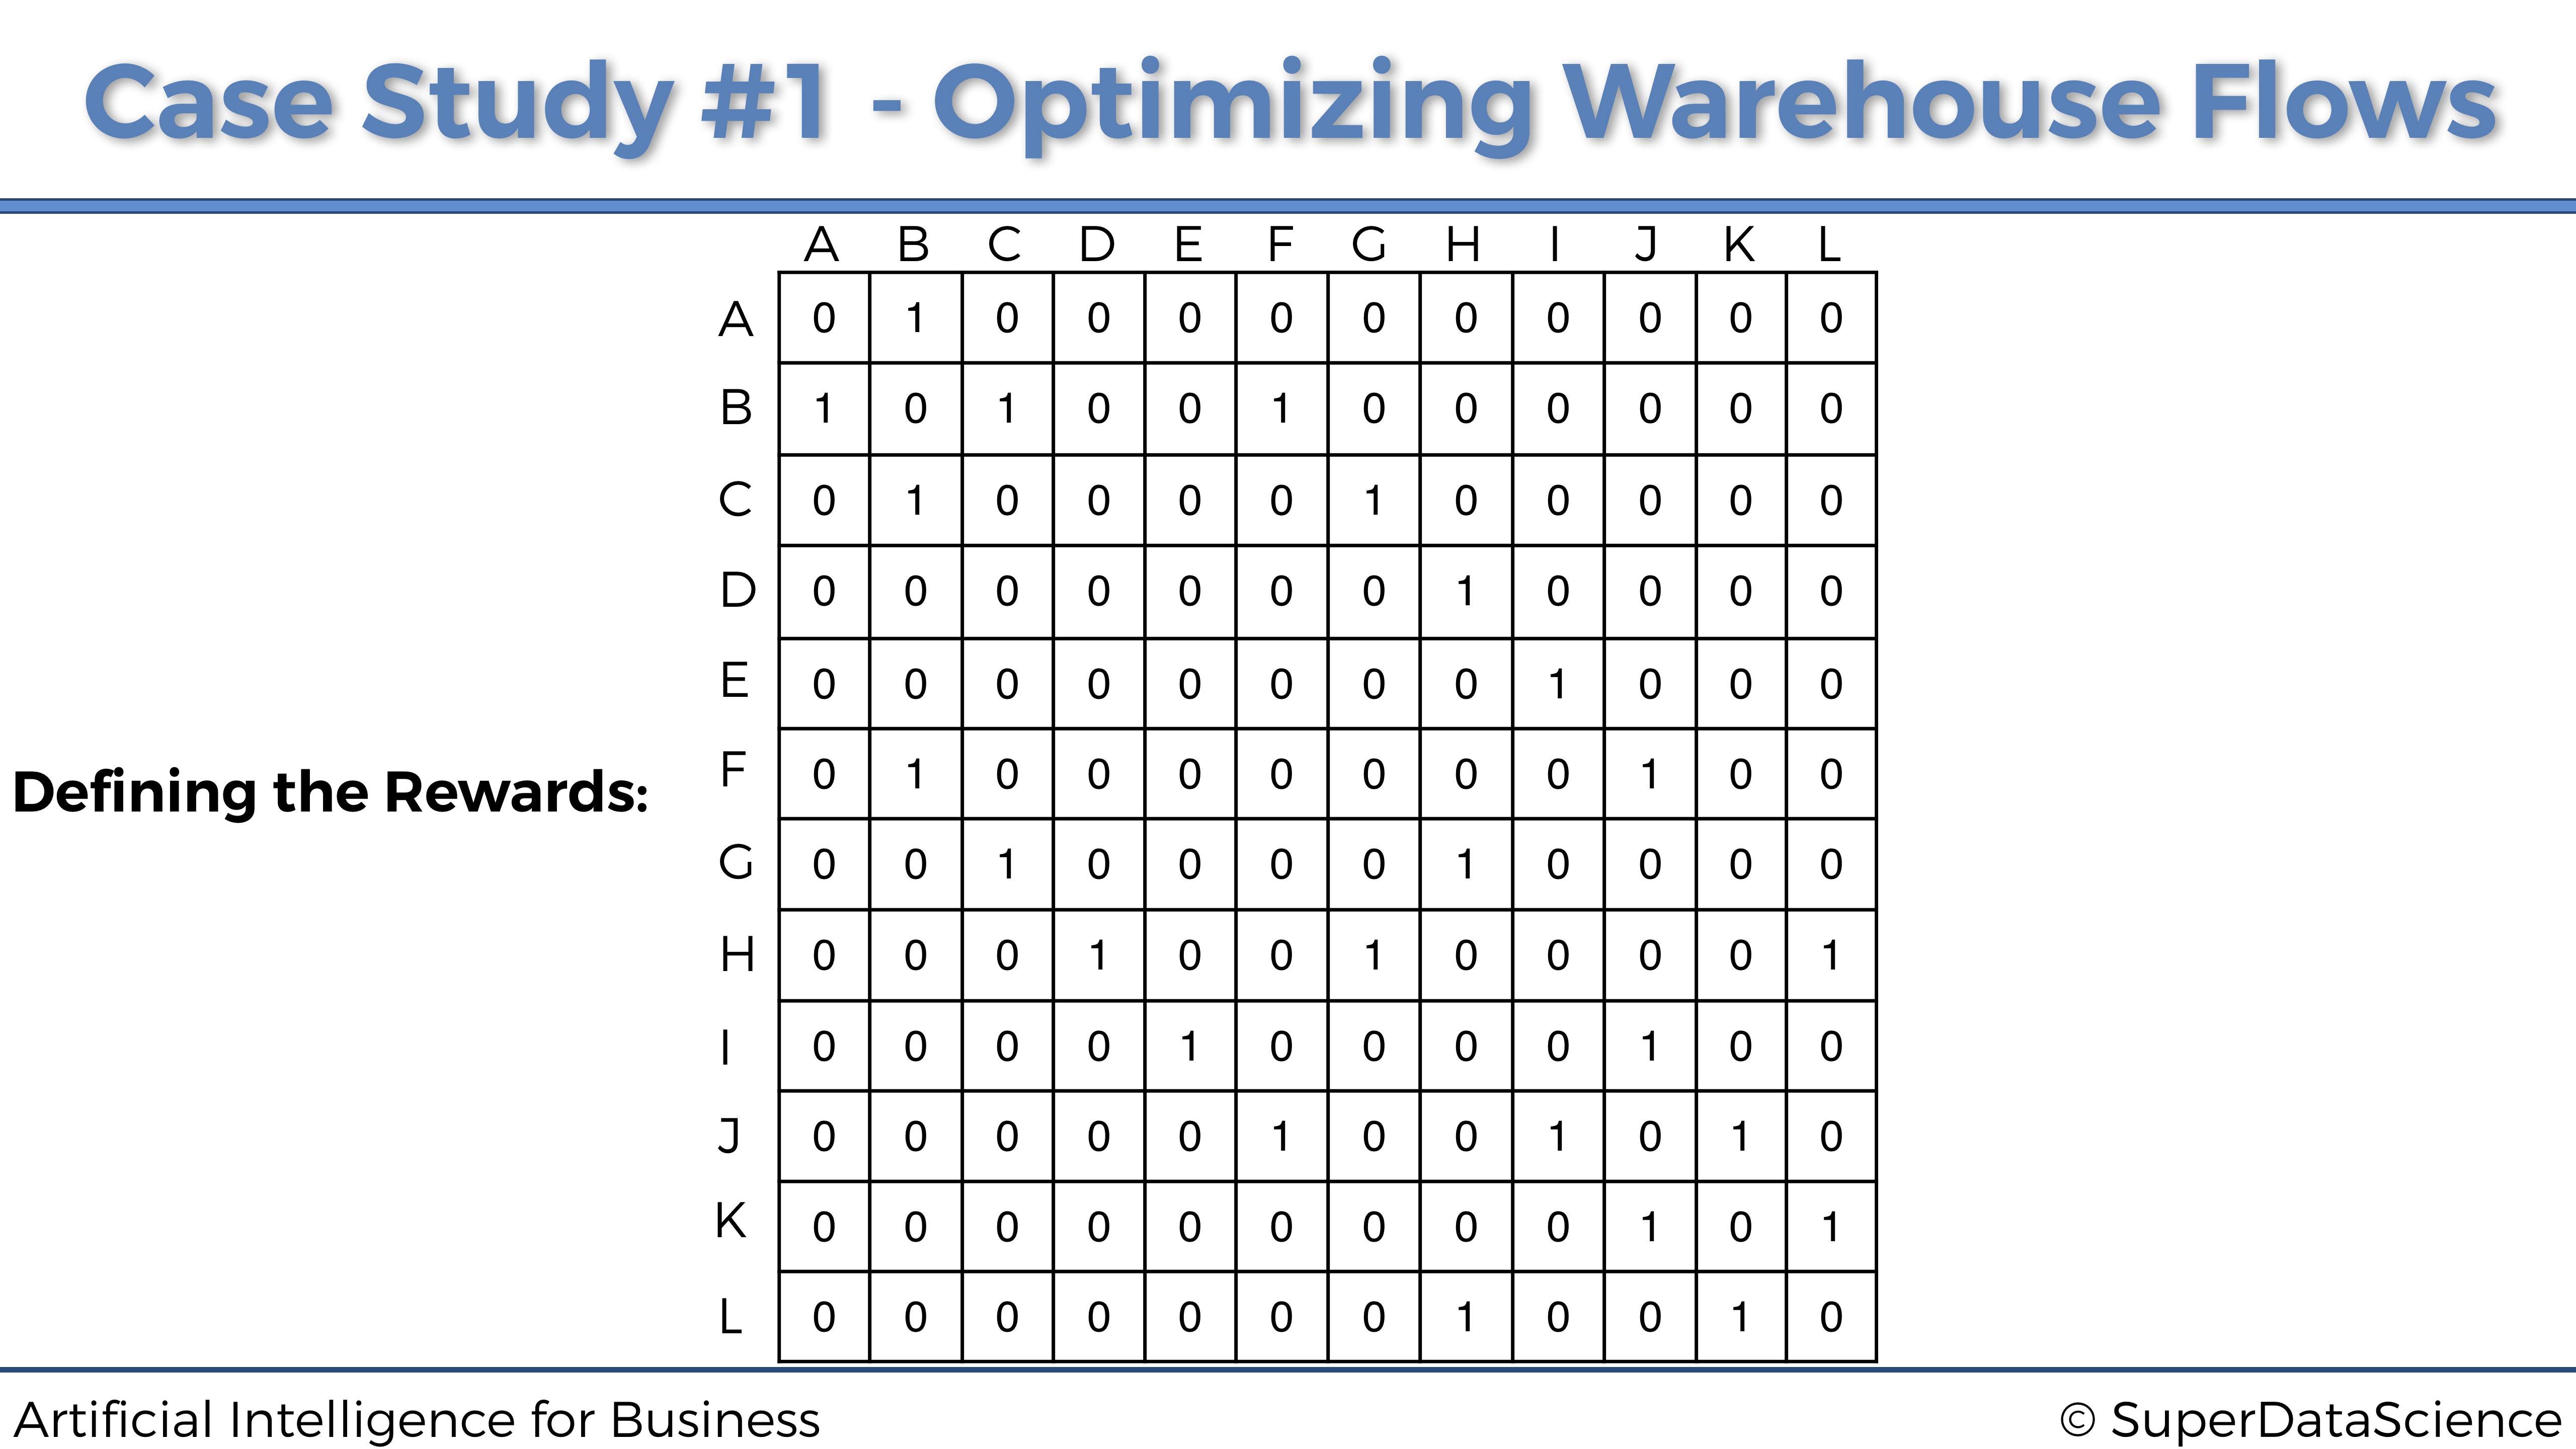
\includegraphics[scale=0.14]{Rewards_Matrix_4.png}
        \end{center}
\end{figure}

Congratulations, we have just defined the rewards. We did it by simply building this matrix of rewards. It is important to understand that this is usually the way we define the system of rewards when doing Q-Learning with a finite number of inputs and actions. In Case Study 2, you will see that we will proceed very differently.

We are almost done, the only thing we need to do left is to attribute high rewards to the top priority locations. This will be done by the computer system that returns the priorities of product collection for each of the 12 locations. Therefore, since location G is the top priority, the computer system will update the matrix of rewards by attributing a high reward in the cell (G,G):

\begin{figure}[!htbp]
        \begin{center}
            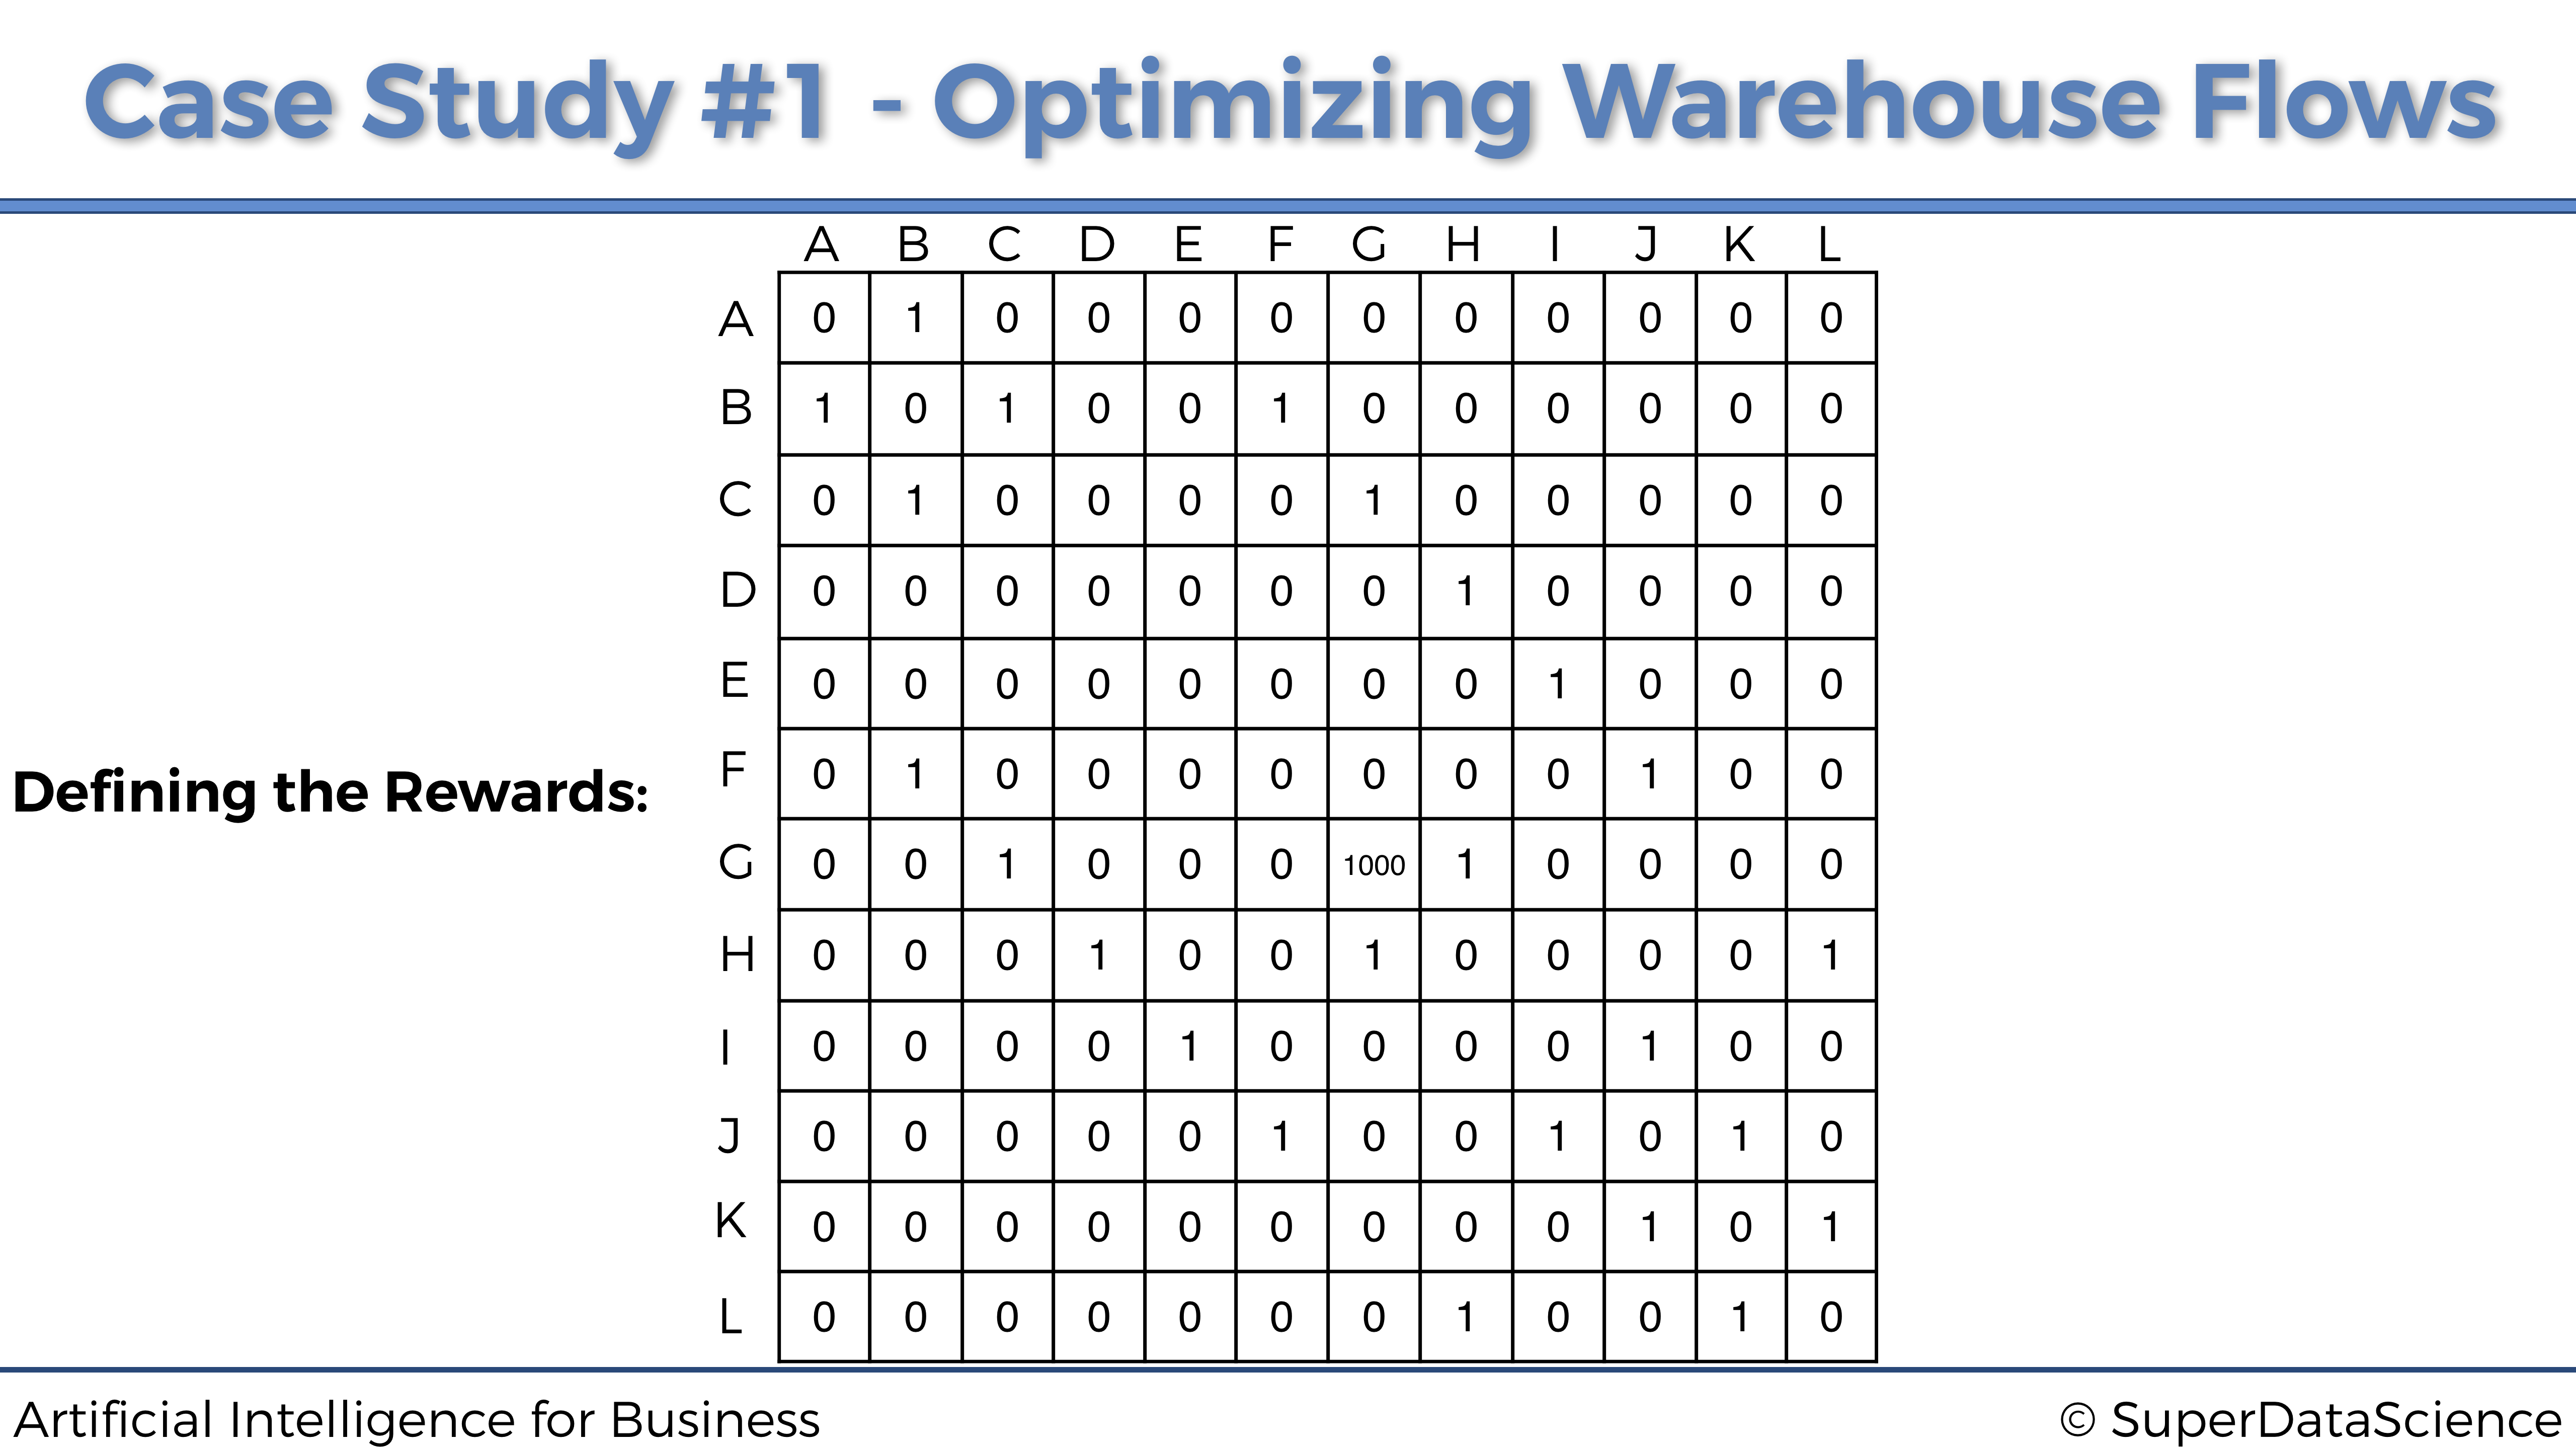
\includegraphics[scale=0.14]{Rewards_Matrix_5.png}
        \end{center}
\end{figure}

And that's how the system of rewards will work with Q-Learning. We attribute the highest reward (here 1000) to the top priority location G. Then you will see in the video lectures how we can attribute a lower high reward to the second top priority location (location K), to make our robot go by this intermediary top priority location, therefore optimizing the warehouse flows.

\subsection{AI Solution}

The AI Solution that will solve the problem described above is a Q-Learning model. Since the latter is based on Markov Decision Processes, or MDPs, we will start by explaining what they are, and then we will move on to the intuition and maths details behind the Q-Learning model.

\subsubsection{Markov Decision Processes}

A Markov Decision Process is a tuple \((S, A, T, R)\) where:

\begin{itemize}

\item $S$ is the set of the different states. Therefore in our case study: $$ S = \{0,1,2,3,4,5,6,7,8,9,10,11\} $$

\item $A$ is the set of the different actions that can be played at each time $t$. Therefore in our case study: $$ A = \{0,1,2,3,4,5,6,7,8,9,10,11\} $$

\item $T$ is called the transition rule:

\begin{equation*}
T : (s_t \in S, s_{t+1} \in S, a_t \in A) \mapsto \mathbb{P}(s_{t+1}|s_t,a_t)
\end{equation*}

where $\mathbb{P}(s_{t+1}|s_t,a_t)$ is the probability to reach the future state $s_{t+1}$ when playing the action $a_t$ in the state $s_t$. Therefore $T$ is the probability distribution of the future states at time $t+1$ given the current state and the action played at time $t$. Accordingly, we can predict the future state $s_{t+1}$ by taking a random draw from that distribution $T$:

\begin{equation*}
s_{t+1} \sim T(s_t,.,a_t) 
\end{equation*}

In our case study, you will see through our implementation that this $T$ distribution of our AI will simply be the uniform distribution, which is a classic choice of distribution working very well when doing Q-Learning.

\item[$\bullet$] $R$ is the reward function:

\begin{equation*}
R : (s_t \in S, a_t \in A) \mapsto r_t \in \mathbb{R}
\end{equation*}

where $r_t$ is the reward obtained after playing the action $a_t$ in the state $s_t$. In our case study, this reward function is exactly the matrix we defined previously.

\end{itemize}

After defining the MDP, it is now important to remind that it relies on the following assumption: the probability of the future state \(s_{t+1}\) only depends on the current state \(s_t\) and action \(a_t\), and doesn't depend on any of the previous states and actions. That is:

\begin{equation*}
\mathbb{P}(s_{t+1}|s_0,a_0,s_1,a_1,...,s_t,a_t) = \mathbb{P}(s_{t+1}|s_t,a_t)
\end{equation*}

Hence in other words, a Markov Decision Process has no memory.

\newpage

Now let's recap what is going on in terms of MDPs. At every time \(t\):

\begin{enumerate}
\item The AI observes the current state $s_t$.
\item The AI plays the action $a_t$.
\item The AI receives the reward $r_t = R(s_t, a_t)$.
\item The AI enters the following state $s_{t+1}$.
\end{enumerate}

So now the question is:

\begin{equation*}
\textbf{How does the AI know which action to play at each time $t$?}
\end{equation*}

To answer this question, we need to introduce the policy function. The policy function \(\pi\) is exactly the function that, given a state \(s_t\), returns the action \(a_t\):

\begin{equation*}
\pi: s_t \in S \mapsto a_t \in A
\end{equation*}

Let's denote by \(\Pi\) the set of all possible policy functions. Then the choice of the best actions to play becomes an optimization problem. Indeed, it comes down to finding the optimal policy \(\pi^*\) that maximizes the accumulated reward:

\begin{equation*}
\pi^* = \underset{\pi \in \Pi}{\textrm{argmax}} \sum_{t \ge 0} R(s_t,\pi(s_t))
\end{equation*}

Therefore of course the question becomes:

\begin{equation*}
\textbf{How to find this optimal policy $\pi^*$ ?}
\end{equation*}

This is where Q-Learning comes into play.

\subsubsection{Q-Learning}

Before we start getting into the details of Q-Learning, we need to explain the concept of the Q-Value.

\textbf{The Q-Value}

To each couple of state and action \((s,a)\), we are going to associate a numeric value \(Q(s,a)\):

\begin{equation*}
Q: (s \in S, a \in A) \mapsto Q(s,a) \in \mathbb{R}
\end{equation*}

We will say that \(Q(s,a)\) is ``the Q-value of the action \(a\) played in the state \(s\)''.

To understand the purpose of this ``Q-Value'', we need to introduce the Temporal Difference.

\textbf{The Temporal Difference}

At the beginning \(t=0\), all the Q-values are initialized to 0:

\begin{equation*}
\forall s \in S, a \in A, Q(s,a) = 0
\end{equation*}

Now let's suppose we are at time \(t\), in a certain state \(s_t\). We play a random action \(a_t\), which brings us to the state \(s_{t+1}\) and we get the reward \(R(s_t,a_t)\).

We can now introduce the Temporal Difference, which is at the heart of Q-Learning. The Temporal Difference at time \(t\), denoted by \(TD_t(s_t,a_t)\), is the difference between:

\begin{itemize}

\item[$\bullet$] $R(s_t,a_t) + \gamma \underset{a}{\max}(Q(s_{t+1},a))$, that is the reward $R(s_t,a_t)$ obtained by playing the action $a_t$ in the state $s_t$, plus the Q-Value of the best action played in the future state $s_{t+1}$, discounted by a factor $\gamma \in [0,1]$, called the discount factor.

\item[$\bullet$] and $Q(s_t, a_t)$, that is the Q-Value of the action $a_t$ played in the state $s_t$,

\end{itemize}

thus leading to:

\begin{equation*}
TD_t(s_t,a_t) = R(s_t,a_t) + \gamma \underset{a}{\max}(Q(s_{t+1},a)) - Q(s_t,a_t)
\end{equation*}

\begin{equation*}
\textbf{OK great, but what exactly is the purpose of this Temporal Difference $TD_t(s_t,a_t)$?}
\end{equation*}

Let's answer this question to give us some better AI intuition. \(TD_t(s_t,a_t)\) is like an intrinsic reward. The AI will learn the Q-values in such a way that:

\begin{itemize}
\item If $TD_t(s_t,a_t)$ is high, the AI gets a "good surprise".
\item If $TD_t(s_t,a_t)$ is small, the AI gets a "frustration".
\end{itemize}

To that extent, the AI will iterate some updates of the Q-Values (through an equation called the Bellman equation) towards higher temporal differences.

Accordingly, in the final next step of the Q-Learning algorithm, we use the Temporal Difference to reinforce the couples (state, action) from time \(t-1\) to time \(t\), according to the following equation:

\begin{equation*}
Q_t(s_t,a_t) = Q_{t-1}(s_t,a_t) + \alpha TD_t(s_t,a_t)
\end{equation*}

where \(\alpha \in \mathbb{R}\) is the learning rate, which dictates how fast the learning of the Q-Values goes, or how big the updates of the Q-Values are. Its value is usually a real number chosen between 0 and 1, like for example 0.01, 0.05, 0.1 or 0.5. The lower is its value, the smaller will be the updates of the Q-Values and the longer will be the Q-Learning. The higher is its value, the bigger will be the updates of the Q-Values and the faster will be the Q-Learning.

This equation above is the Bellman equation. It is the pillar of Q-Learning.

With this point of view, the Q-Values measure the accumulation of surprise or frustration associated with the couple of action and state \((s_t,a_t)\). In the surprise case, the AI is reinforced, and in the frustration case, the AI is weakened. Hence we want to learn the Q-Values that will give the AI the maximum ``good surprise''.

Accordingly, the decision of which action to play mostly depends on the Q-value \(Q(s_t, a_t)\). If the action \(a_t\) played in the state \(s_t\) is associated with a high Q-Value \(Q(s_t,a_t)\), the AI will have a higher tendency to choose \(a_t\). On the other hand if the action \(a_t\) played in the state \(s_t\) is associated with a small Q-value \(Q(s_t, a_t)\), the AI will have a smaller tendency to choose \(a_t\).

There are several ways of choosing the best action to play. First, when being in a certain state \(s_t\), we could simply take the action \(a_t\) that maximizes the Q-Value \(Q(s_t,a_t)\):

\begin{equation*}
a_t = \underset{a}{\textrm{argmax}}(Q(s_t,a))
\end{equation*}

This solution is the Argmax method.

Another great solution, which turns out to be an even better solution for complex problems, is the Softmax method.

The Softmax method consists of considering for each state \(s\) the following distribution:

\begin{equation*}
W_s: a \in A \mapsto \frac{\exp(Q(s,a))^{\tau}}{\sum_{a'}\exp(Q(s,a'))^{\tau}} \textrm{ with } \tau \ge 0
\end{equation*}

Then we choose which action \(a\) to play by taking a random draw from that distribution:

\begin{equation*}
a \sim W_s(.)
\end{equation*}

However the problem we will solve in Case Study 1 will be simple enough to use the Argmax method, so this is what we will choose.

\subsubsection{The whole Q-Learning algorithm}

Let's summarize the different steps of the whole Q-Learning process:

\textbf{Initialization}:

For all couples of states \(s\) and actions \(a\), the Q-Values are initialized to 0:

\begin{equation*}
\forall s \in S, a \in A, Q_0(s,a) = 0
\end{equation*}

We start in the initial state \(s_0\). We play a random possible action and we reach the first state \(s_1\).

\textbf{Then for each $t \ge 1$}, we will repeat for a certain number of times (1000 times in our code) the following:

\begin{enumerate}

\item We select a random state $s_t$ from our 12 possible states:

\begin{equation*}
    s_t = \textrm{random}(0,1,2,3,4,5,6,7,8,9,10,11)
\end{equation*}

\item We play a random action $a_t$ that can lead to a next possible state, i.e., such that $R(s_t,a_t) > 0$:

\begin{equation*}
a_t = \textrm{random}(0,1,2,3,4,5,6,7,8,9,10,11) \textrm{ s.t. } R(s_t,a_t) > 0
\end{equation*}

\item We reach the next state $s_{t+1}$ and we get the reward $R(s_t,a_t)$

\item We compute the Temporal Difference $TD_t(s_t,a_t)$:

\begin{equation*}
TD_t(s_t,a_t) = R(s_t,a_t) + \gamma \underset{a}{\max}(Q(s_{t+1},a)) - Q(s_t, a_t)
\end{equation*}

\item We update the Q-value by applying the Bellman equation:

\begin{equation*}
Q_t(s_t,a_t) = Q_{t-1}(s_t,a_t) + \alpha TD_t(s_t,a_t)
\end{equation*}

\end{enumerate}

\newpage

\subsection{Implementation}

Now let's provide and explain the whole implementation of this Q-Learning model, the solution of our warehouse flows optimization problem.

First, we start by importing the libraries that will be used in this implementation. These only include the numpy library, which offers a practical way of working with arrays and mathematical operations:

\begin{lstlisting}
# Importing the libraries
import numpy as np
\end{lstlisting}

Then we set the parameters of our model. These include the discount factor \(\gamma\) and the learning rate \(\alpha\), which as we saw in Section 1.2, are the only parameters of the Q-Learning algorithm:

\begin{lstlisting}
# Setting the parameters gamma and alpha for the Q-Learning
gamma = 0.75
alpha = 0.9
\end{lstlisting}

The two previous code sections were simply the introductory sections, before really starting to build our AI model. Now the next step is to start the first part of our implementation: Part 1 - Defining the Environment. And for that of course, we begin by defining the states, with a dictionary mapping the locations names (in letters from A to L) into the states (in indexes from 0 to 11):

\begin{lstlisting}
# PART 1 - DEFINING THE ENVIRONMENT

# Defining the states
location_to_state = {'A': 0,
                     'B': 1,
                     'C': 2,
                     'D': 3,
                     'E': 4,
                     'F': 5,
                     'G': 6,
                     'H': 7,
                     'I': 8,
                     'J': 9,
                     'K': 10,
                     'L': 11}
\end{lstlisting}

Then we define the actions, with a simple list of indexes from 0 to 11. Remember that each action index corresponds to the next state (next location) where that action leads to:

\begin{lstlisting}
# Defining the actions
actions = [0,1,2,3,4,5,6,7,8,9,10,11]
\end{lstlisting}

And eventually, we define the rewards, by creating a matrix of rewards, where the rows correspond to the current states \(s_t\), the columns correspond to the actions \(a_t\) leading to the next state \(s_{t+1}\), and the cells contain the rewards \(R(s_t,a_t)\). If a cell \((s_t,a_t)\) has a 1, that means that we can play the action \(a_t\) from the current state \(s_t\) to reach the next state \(s_{t+1}\). If a cell \((s_t,a_t)\) has a 0, that means that we cannot play the action \(a_t\) from the current state \(s_t\) to reach any next state \(s_{t+1}\). And for now we will manually put a high reward (1000) inside the cell corresponding to location G, because it is the top priority location where the autonomous warehouse has to go to collect the products. Since location G has encoded index state 6, we put a 1000 reward on the cell of row 6 and column 6. Then later on we will improve our solution by implementing an automatic way of going to the top priority location, without having to manually update the matrix of rewards and leaving it initialized with 0s and 1s just as it should be. But in the meantime, here is below our matrix of rewards including the manual update:

\begin{lstlisting}
# Defining the rewards
R = np.array([[0,1,0,0,0,0,0,0,0,0,0,0],
              [1,0,1,0,0,1,0,0,0,0,0,0],
              [0,1,0,0,0,0,1,0,0,0,0,0],
              [0,0,0,0,0,0,0,1,0,0,0,0],
              [0,0,0,0,0,0,0,0,1,0,0,0],
              [0,1,0,0,0,0,0,0,0,1,0,0],
              [0,0,1,0,0,0,1000,1,0,0,0,0],
              [0,0,0,1,0,0,1,0,0,0,0,1],
              [0,0,0,0,1,0,0,0,0,1,0,0],
              [0,0,0,0,0,1,0,0,1,0,1,0],
              [0,0,0,0,0,0,0,0,0,1,0,1],
              [0,0,0,0,0,0,0,1,0,0,1,0]])
\end{lstlisting}

That closes this first part. Now let's begin the second part of our implementation: Part 2 - Building the AI Solution with Q-Learning. To that extent, we are going to follow the Q-Learning algorithm exactly as it was provided in Section 1.2. Hence we first initialize all the Q-Values, by creating our matrix of Q-Values full of zeros (in which same, the rows correspond to the current states \(s_t\), the columns correspond to the actions \(a_t\) leading to the next state \(s_{t+1}\), and the cells contain the Q-Values \(Q(s_t,a_t))\):

\begin{lstlisting}
# PART 2 - BUILDING THE AI SOLUTION WITH Q-LEARNING

# Initializing the Q-Values
Q = np.array(np.zeros([12,12]))
\end{lstlisting}

Then of course we implement the Q-Learning process, with a for loop over 1000 iterations, repeating 1000 times the steps of the Q-Learning process provided at the end of Section 1.2:

\begin{lstlisting}
# Implementing the Q-Learning process
for i in range(1000):
    current_state = np.random.randint(0,12)
    playable_actions = []
    for j in range(12):
        if R[current_state, j] > 0:
            playable_actions.append(j)
    next_state = np.random.choice(playable_actions)
    TD = R[current_state, next_state] + gamma*Q[next_state, np.argmax(Q[next_state,])]
         - Q[current_state, next_state]
    Q[current_state, next_state] = Q[current_state, next_state] + alpha*TD
\end{lstlisting}

Optional: at this stage of the code, our matrix of Q-Values is ready. We can have a look at it by executing the whole code we have implemented so far, and by entering the following print in the console:

\begin{lstlisting}
print("Q-Values:")
print(Q.astype(int))
\end{lstlisting}

And we obtain the following matrix of final Q-Values:

\begin{figure}[!htbp]
        \begin{center}
            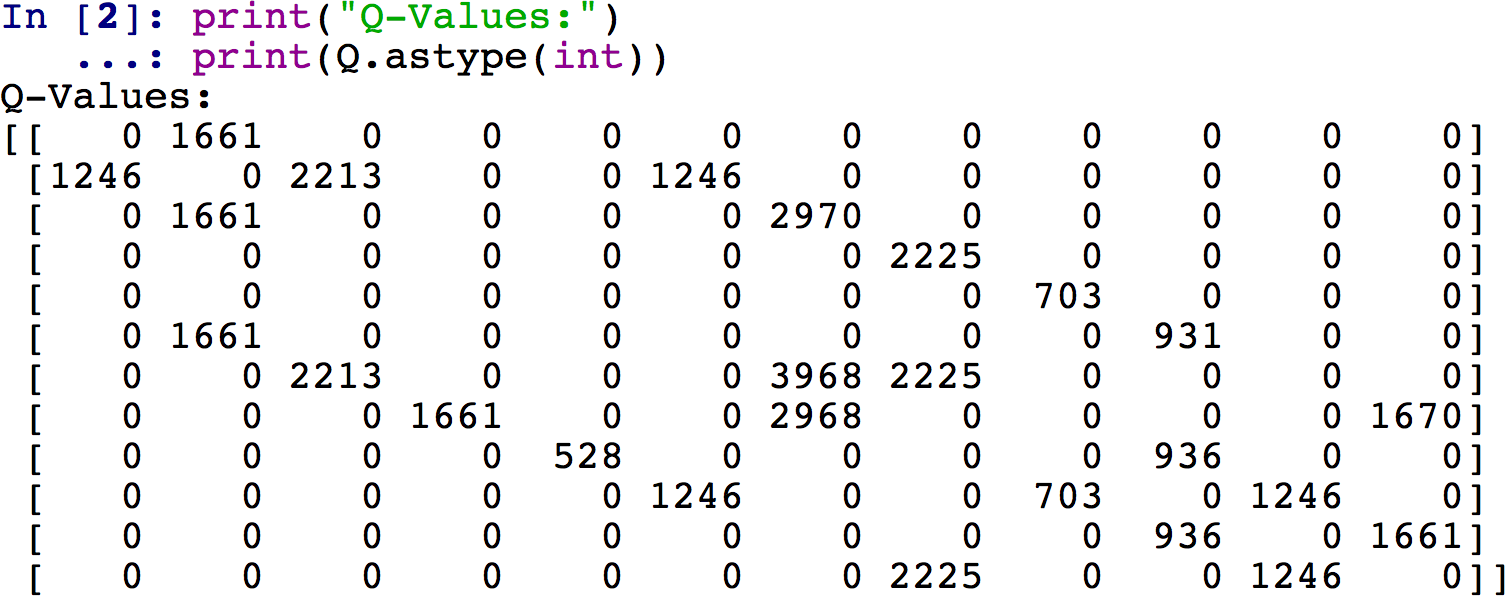
\includegraphics[scale=0.5]{Q_Values_Console.png}
        \end{center}
\end{figure}

For more visual clarity, you can even check the matrix of Q-Values directly in Variable Explorer, by double clicking on Q. Then to get the Q-Values as integers you can click on ``Format'' and inside enter a float formatting of ``\%.0f''. You will obtain this, which is a bit more clear since you can see the indexes of the rows and columns in your matrix Q:

\begin{figure}[!htbp]
        \begin{center}
            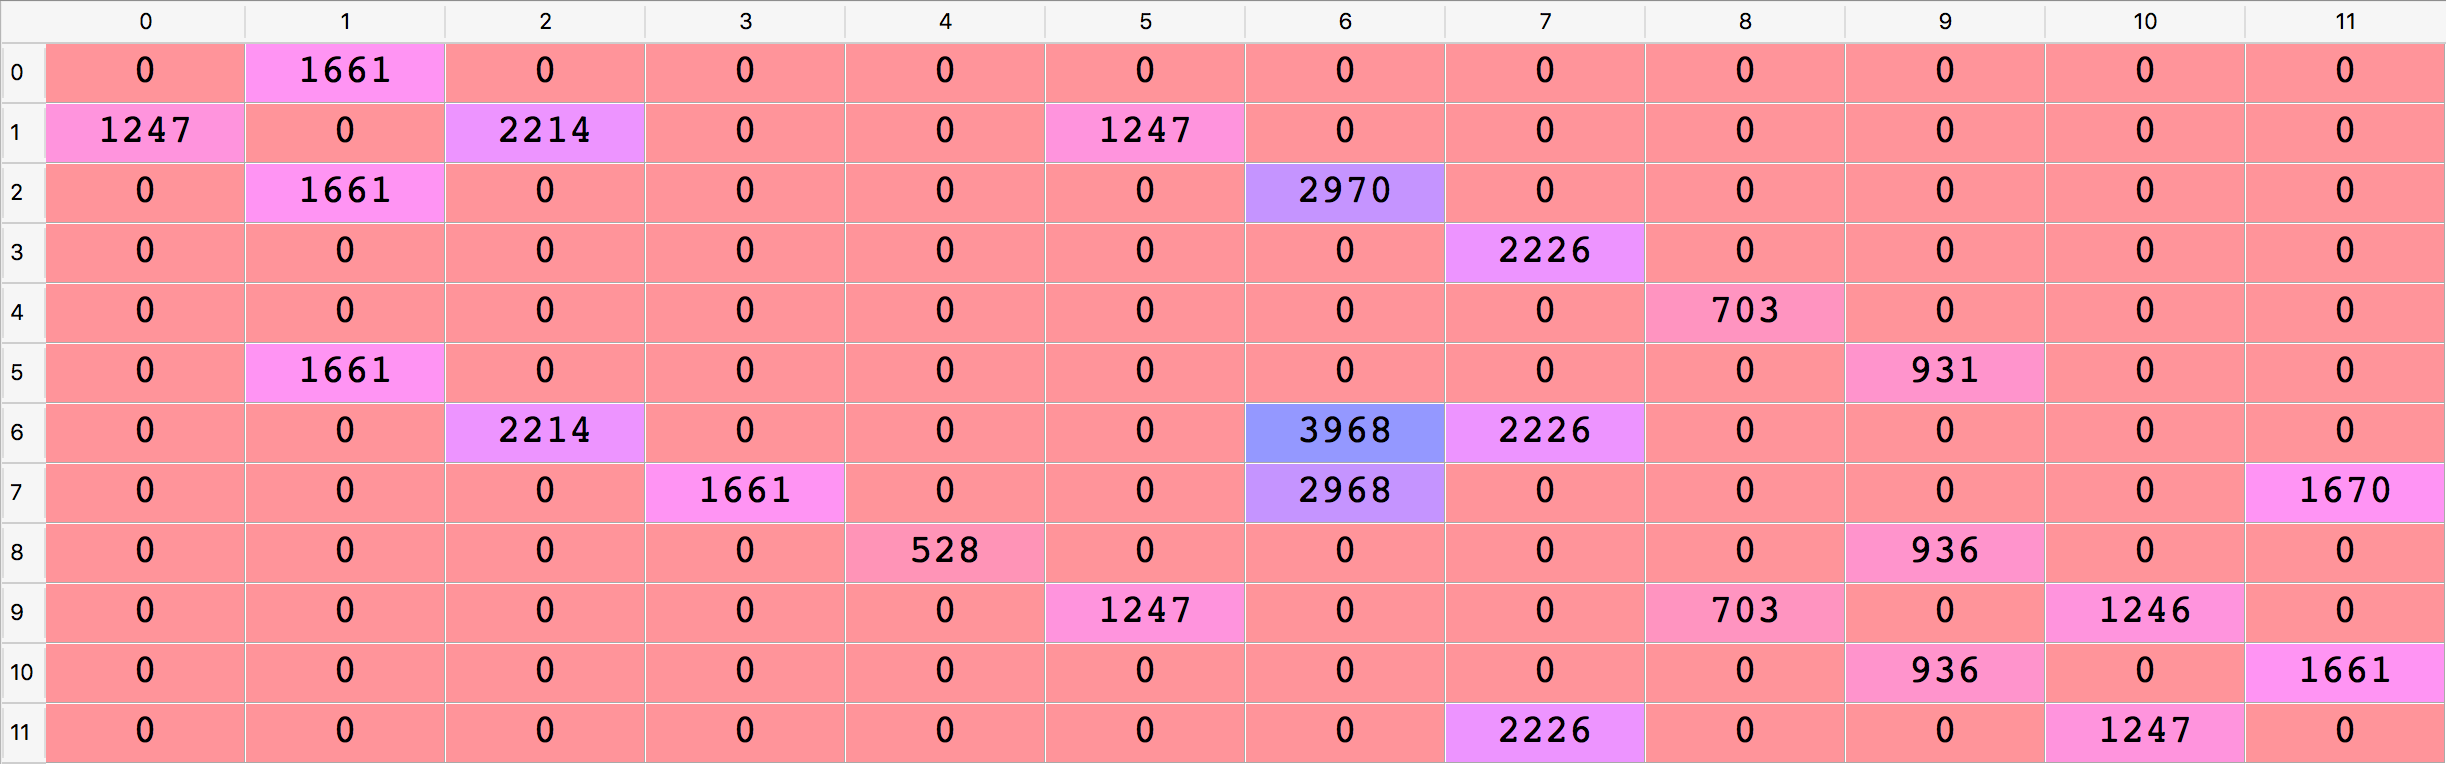
\includegraphics[scale=0.35]{Q_Values_Variable_Explorer.png}
        \end{center}
\end{figure}

Good, now that we have our matrix of Q-Values, we are ready to go into production! Hence we can move on to the third part of the implementation, Part 3 - Going into Production, inside which we will compute the optimal path from any starting location to any ending top priority location. The idea here will be to implement a ``route'' function, that will take as inputs the starting location where our autonomous warehouse robot is located at a specific time and the ending location where it has to go in top priority, and that will return as output the shortest route inside a list. However since we want to input the locations with there names (in letters), as opposed to their states (in indexes), we will need a dictionary that maps the locations states (in indexes) to the locations names (in letters). And that is the first thing we will do here in this third part, using a trick to inverse our previous dictionary ``location\_to\_state'', since indeed we simply want to get the exact inverse mapping from this dictionary:

\begin{lstlisting}
# PART 3 - GOING INTO PRODUCTION

# Making a mapping from the states to the locations
state_to_location = {state: location for location, state in location_to_state.items()}
\end{lstlisting}

This is when the most important code section comes into play. We are about to implement the final ``route()'' function that will take as inputs the starting and ending locations, and that will return the optimal path between these two locations. To explain exactly what this route function will do, let's enumerate the different steps of the process, when going from location E to location G:

\begin{enumerate}
    \item We start at our starting location E.
    \item We get the state of location E, which according to our location\_to\_state mapping is $s_0 = 4$.
    \item On the row of index $s_0 = 4$ in our matrix of Q-Values, we find the column that has the maximum Q-Value (703).
    \item This column has index 8, so we play the action of index 8 which leads us to the next state $s_{t+1} = 8$.
    \item We get the location of state 8, which according to our state\_to\_location mapping is location I. Hence our next location is location I, which is appended to our list containing the optimal path.
    \item We repeat the same previous 5-steps from our new starting location I, until we reach our final destination, location G.
\end{enumerate}

Hence, since we don't know how many locations we will have to go through between the starting and ending locations, we have to make a while loop that will repeat the 5-steps process described above, and that will stop as soon as we reach the ending top priority location:

\begin{lstlisting}
# Making the final function that will return the optimal route
def route(starting_location, ending_location):
    route = [starting_location]
    next_location = starting_location
    while (next_location != ending_location):
        starting_state = location_to_state[starting_location]
        next_state = np.argmax(Q[starting_state,])
        next_location = state_to_location[next_state]
        route.append(next_location)
        starting_location = next_location
    return route
\end{lstlisting}

Congratulations, our tool is now ready! When we test it to go from E to G, we get indeed the two possible optimal paths after printing the final route executing the whole code several times:

\begin{lstlisting}
# Printing the final route
print('Route:')
route('E', 'G')

Route:
Out[1]: ['E', 'I', 'J', 'F', 'B', 'C', 'G']
Out[2]: ['E', 'I', 'J', 'K', 'L', 'H', 'G']
\end{lstlisting}

Good, we have a first version of the model that is well functioning. But we can improve it in two ways. First, by automating the reward attribution to the top priority location, so that we don't have to do it manually. And second, by adding a feature that gives us the option to go by an intermediary location before going to the top priority location. That intermediary location should be of course in the Top 3 priority locations. And as a matter of fact, in our top priority locations ranking, the second top priority location is location K. Therefore, in order to optimize even more the warehouse flows, our autonomous warehouse robot must go by location K to collect the products on its way to the top priority location G. A way to do this is to have the option to go by any intermediary location in the process of our ``route()'' function. And this is exactly what we will implement as a second improvement. But first, let's implement the first improvement, that automates the reward attribution.

The way to do that is two folds: first we must make a copy (called R\_new) of our reward matrix inside which the route() function will automatically update the reward in the cell of the ending location. Indeed, the ending location is one of the inputs of the route() function, so using our location\_to\_state dictionary we can very easily find that cell and update its reward to 1000. And second, we must include the whole Q-Learning algorithm (including the initialization step) inside the route function, right after we make that update of the reward in our copy of the rewards matrix. Indeed, in our previous implementation above, the Q-Learning process happens on the original version of the rewards matrix, which is now supposed to stay as it is, i.e.~initialized to 1s and 0s only. Therefore we must include the Q-Learning process inside the route function, and make it happen on our copy R\_new of the rewards matrix, instead of the original rewards matrix R. Hence, our full implementation becomes the following:

\begin{lstlisting}
# Artificial Intelligence for Business
# Optimizing Warehouse Flows with Q-Learning

# Importing the libraries
import numpy as np

# Setting the parameters gamma and alpha for the Q-Learning
gamma = 0.75
alpha = 0.9

# PART 1 - DEFINING THE ENVIRONMENT

# Defining the states
location_to_state = {'A': 0,
                     'B': 1,
                     'C': 2,
                     'D': 3,
                     'E': 4,
                     'F': 5,
                     'G': 6,
                     'H': 7,
                     'I': 8,
                     'J': 9,
                     'K': 10,
                     'L': 11}

# Defining the actions
actions = [0,1,2,3,4,5,6,7,8,9,10,11]

# Defining the rewards
R = np.array([[0,1,0,0,0,0,0,0,0,0,0,0],
              [1,0,1,0,0,1,0,0,0,0,0,0],
              [0,1,0,0,0,0,1,0,0,0,0,0],
              [0,0,0,0,0,0,0,1,0,0,0,0],
              [0,0,0,0,0,0,0,0,1,0,0,0],
              [0,1,0,0,0,0,0,0,0,1,0,0],
              [0,0,1,0,0,0,1,1,0,0,0,0],
              [0,0,0,1,0,0,1,0,0,0,0,1],
              [0,0,0,0,1,0,0,0,0,1,0,0],
              [0,0,0,0,0,1,0,0,1,0,1,0],
              [0,0,0,0,0,0,0,0,0,1,0,1],
              [0,0,0,0,0,0,0,1,0,0,1,0]])

# PART 2 - BUILDING THE AI SOLUTION WITH Q-LEARNING

# Making a mapping from the states to the locations
state_to_location = {state: location for location, state in location_to_state.items()}

# Making the final function that will return the route
def route(starting_location, ending_location):
    R_new = np.copy(R)
    ending_state = location_to_state[ending_location]
    R_new[ending_state, ending_state] = 1000
    Q = np.array(np.zeros([12,12]))
    for i in range(1000):
        current_state = np.random.randint(0,12)
        playable_actions = []
        for j in range(12):
            if R_new[current_state, j] > 0:
                playable_actions.append(j)
        next_state = np.random.choice(playable_actions)
        TD = R_new[current_state, next_state]
             + gamma * Q[next_state, np.argmax(Q[next_state,])]
             - Q[current_state, next_state]
        Q[current_state, next_state] = Q[current_state, next_state] + alpha * TD
    route = [starting_location]
    next_location = starting_location
    while (next_location != ending_location):
        starting_state = location_to_state[starting_location]
        next_state = np.argmax(Q[starting_state,])
        next_location = state_to_location[next_state]
        route.append(next_location)
        starting_location = next_location
    return route

# PART 3 - GOING INTO PRODUCTION

# Printing the final route
print('Route:')
route('E', 'G')
\end{lstlisting}

By executing this new code several times, we get of course the same two possible optimal paths as before.

Now let's tackle the second improvement. There are three ways to add the option of going by the intermediary location K, the second top priority location:

\begin{enumerate}
    \item We give a high reward to the action leading from location J to location K. This high reward has to be larger than 1, and below 1000. Indeed it has to be larger than 1 so that the Q-Learning process favors the action leading from J to K, as opposed to the action leading from J to F which has reward 1. And it must be below than 1000 so we have to keep the highest reward on the top priority location, to make sure we end up there. Hence for example, in our rewards matrix we can give a high reward of 500 to the cell in the row of index 9 and the column of index 10, since indeed that cell corresponds to the action leading from location J (state index 9) to location K (state index 10). That way our autonomous warehouse robot will always go by location K on its way to location G. Here is how the matrix of rewards would be in that case:
    \begin{lstlisting}
    # Defining the rewards
    R = np.array([[0,1,0,0,0,0,0,0,0,0,0,0],
              [1,0,1,0,0,1,0,0,0,0,0,0],
              [0,1,0,0,0,0,1,0,0,0,0,0],
              [0,0,0,0,0,0,0,1,0,0,0,0],
              [0,0,0,0,0,0,0,0,1,0,0,0],
              [0,1,0,0,0,0,0,0,0,1,0,0],
              [0,0,1,0,0,0,1,1,0,0,0,0],
              [0,0,0,1,0,0,1,0,0,0,0,1],
              [0,0,0,0,1,0,0,0,0,1,0,0],
              [0,0,0,0,0,1,0,0,1,0,500,0],
              [0,0,0,0,0,0,0,0,0,1,0,1],
              [0,0,0,0,0,0,0,1,0,0,1,0]])
    \end{lstlisting}
    \item We give a bad reward to the action leading from location J to location F. This bad reward just has to be below 0. Indeed by punishing this action with a bad reward the Q-Learning process will never favor that action leading from J to F. Hence for example, in our rewards matrix we can give a bad reward of -500 to the cell in the row of index 9 and the column of index 5, since indeed that cell corresponds to the action leading from location J (state index 9) to location F (state index 5). That way our autonomous warehouse robot will never go trough location F on its way to location G. Here is how the matrix of rewards would be in that case:
    \begin{lstlisting}
    # Defining the rewards
    R = np.array([[0,1,0,0,0,0,0,0,0,0,0,0],
              [1,0,1,0,0,1,0,0,0,0,0,0],
              [0,1,0,0,0,0,1,0,0,0,0,0],
              [0,0,0,0,0,0,0,1,0,0,0,0],
              [0,0,0,0,0,0,0,0,1,0,0,0],
              [0,1,0,0,0,0,0,0,0,1,0,0],
              [0,0,1,0,0,0,1,1,0,0,0,0],
              [0,0,0,1,0,0,1,0,0,0,0,1],
              [0,0,0,0,1,0,0,0,0,1,0,0],
              [0,0,0,0,0,-500,0,0,1,0,1,0],
              [0,0,0,0,0,0,0,0,0,1,0,1],
              [0,0,0,0,0,0,0,1,0,0,1,0]])
    \end{lstlisting}
    \item We make an additional best\_route() function, taking as inputs the three starting, intermediary and ending locations, that will call our previous route() function twice, a first time from the starting location to the intermediary location, and a second time from the intermediary location to the ending location.
\end{enumerate}

The first two ideas are easy to implement manually, but very tricky to implement automatically. Indeed, it is easy to find automatically the index of the intermediary location where we want to go by, but very difficult to get the index of the location that leads to that intermediary location, since it depends on the starting location and the ending location. You can try to implement either the first or second idea, you will see what I mean. Accordingly, we will implement the third idea, which can be coded in just two extra lines of code:

\begin{lstlisting}
# Making the final function that returns the optimal route
def best_route(starting_location, intermediary_location, ending_location):
    return route(starting_location, intermediary_location)
           + route(intermediary_location, ending_location)[1:]
\end{lstlisting}

Eventually, the final code including that major improvement for our warehouse flows optimization, becomes:

\begin{lstlisting}
# Artificial Intelligence for Business
# Optimizing Warehouse Flows with Q-Learning

# Importing the libraries
import numpy as np

# Setting the parameters gamma and alpha for the Q-Learning
gamma = 0.75
alpha = 0.9

# PART 1 - DEFINING THE ENVIRONMENT

# Defining the states
location_to_state = {'A': 0,
                     'B': 1,
                     'C': 2,
                     'D': 3,
                     'E': 4,
                     'F': 5,
                     'G': 6,
                     'H': 7,
                     'I': 8,
                     'J': 9,
                     'K': 10,
                     'L': 11}

# Defining the actions
actions = [0,1,2,3,4,5,6,7,8,9,10,11]

# Defining the rewards
R = np.array([[0,1,0,0,0,0,0,0,0,0,0,0],
              [1,0,1,0,0,1,0,0,0,0,0,0],
              [0,1,0,0,0,0,1,0,0,0,0,0],
              [0,0,0,0,0,0,0,1,0,0,0,0],
              [0,0,0,0,0,0,0,0,1,0,0,0],
              [0,1,0,0,0,0,0,0,0,1,0,0],
              [0,0,1,0,0,0,1,1,0,0,0,0],
              [0,0,0,1,0,0,1,0,0,0,0,1],
              [0,0,0,0,1,0,0,0,0,1,0,0],
              [0,0,0,0,0,1,0,0,1,0,1,0],
              [0,0,0,0,0,0,0,0,0,1,0,1],
              [0,0,0,0,0,0,0,1,0,0,1,0]])

# PART 2 - BUILDING THE AI SOLUTION WITH Q-LEARNING

# Making a mapping from the states to the locations
state_to_location = {state: location for location, state in location_to_state.items()}

# Making a function that returns the shortest route from a starting to ending location
def route(starting_location, ending_location):
    R_new = np.copy(R)
    ending_state = location_to_state[ending_location]
    R_new[ending_state, ending_state] = 1000
    Q = np.array(np.zeros([12,12]))
    for i in range(1000):
        current_state = np.random.randint(0,12)
        playable_actions = []
        for j in range(12):
            if R_new[current_state, j] > 0:
                playable_actions.append(j)
        next_state = np.random.choice(playable_actions)
        TD = R_new[current_state, next_state]
             + gamma * Q[next_state, np.argmax(Q[next_state,])]
             - Q[current_state, next_state]
        Q[current_state, next_state] = Q[current_state, next_state] + alpha * TD
    route = [starting_location]
    next_location = starting_location
    while (next_location != ending_location):
        starting_state = location_to_state[starting_location]
        next_state = np.argmax(Q[starting_state,])
        next_location = state_to_location[next_state]
        route.append(next_location)
        starting_location = next_location
    return route

# PART 3 - GOING INTO PRODUCTION

# Making the final function that returns the optimal route
def best_route(starting_location, intermediary_location, ending_location):
    return route(starting_location, intermediary_location)
           + route(intermediary_location, ending_location)[1:]

# Printing the final route
print('Route:')
best_route('E', 'K', 'G')
\end{lstlisting}

By executing this whole new code as many times as we want, we will always get the same expected output:

\begin{lstlisting}
Best Route:
Out[1]: ['E', 'I', 'J', 'K', 'L', 'H', 'G']
\end{lstlisting}

\hypertarget{part-2---minimizing-costs}{%
\chapter{Part 2 - Minimizing Costs}\label{part-2---minimizing-costs}}

Congratulations for smashing the first case study! Let's move on to a brand new and more advanced AI.

\hypertarget{case-study-minimizing-costs-in-energy-consumption-of-a-data-center}{%
\section{Case Study: Minimizing Costs in Energy Consumption of a Data Center}\label{case-study-minimizing-costs-in-energy-consumption-of-a-data-center}}

\hypertarget{problem-to-solve-1} using their DQN AI model (Deep Q-Learning). In this case study, we will do something very similar. We will set up our own server environment, and we will build an AI that will be controlling the cooling/heating of the server so that it stays in an optimal range of temperatures while saving the maximum energy, therefore minimizing the costs. And just as DeepMind AI did, our goal will be to achieve at least 40\% energy saving.

\subsubsection{Environment to define}

Before we define the states, actions and rewards, we need to explain how the server operates. We will do that in several steps. First, we will list all the environment parameters and variables by which the server is controlled. After that we will set the essential assumption of the problem, on which our AI will rely to provide a solution. Then we will specify how we will simulate the whole process. And eventually we will explain the overall functioning of the server, and how the AI plays its role.

\textbf{Parameters:}

\begin{itemize}
    \item the average atmospheric temperature over a month
    \item the optimal range of temperatures of the server, which will be $[18 \degree \textrm{C}, 24 \degree \textrm{C}]$
    \item the minimum temperature of the server below which it fails to operate, which will be $-20 \degree \textrm{C}$
    \item the maximum temperature of the server above which it fails to operate, which will be $80 \degree \textrm{C}$
    \item the minimum number of users in the server, which will be 10
    \item the maximum number of users in the server, which will be 100
    \item the maximum number of users in the server that can go up or down per minute, which will be 5
    \item the minimum rate of data transmission in the server, which will be 20
    \item the maximum rate of data transmission in the server, which will be 300
    \item the maximum rate of data transmission that can go up or down per minute, which will be 10
\end{itemize}

\textbf{Variables:}

\begin{itemize}
    \item the temperature of the server at any minute
    \item the number of users in the server at any minute
    \item the rate of data transmission at any minute
    \item the energy spent by the AI onto the server (to cool it down or heat it up) at any minute
    \item the energy spent by the server's integrated cooling system that automatically brings the server's temperature back to the optimal range whenever the server's temperature goes outside this optimal range
\end{itemize}

All these parameters and variables will be part of our server environment and will influence the actions of the AI on the server.

Then let's give and explain below the two core assumptions of the environment. It is important to understand that these assumptions are not AI related, but just used to simplify the environment so that we can focus the maximum on the AI solution.

\textbf{Assumptions:}

We will rely on the following two essential assumptions:

\textbf{Assumption 1: The temperature of the server can be approximated through Multiple Linear Regression, by a linear function of the atmospheric temperature, the number of users and the rate of data transmission}:

\begin{equation*}
    \textrm{server temperature} = b_0 + b_1 \times \textrm{atmospheric temperature} + b_2 \times \textrm{number of users} + b_3 \times \textrm{data transmission rate} 
\end{equation*}

where \(b_0 \in \mathbb{R}\), \(b_1>0\), \(b_2>0\) and \(b_3>0\).

The raison d'être of this assumption and the reason why \(b_1>0\), \(b_2>0\) and \(b_3>0\) are intuitive to understand. Indeed, it makes sense that when the atmospheric temperature increases, the temperature of the server increases. Also, the more users are active in the server, the more the server has to spend energy to handle them and therefore the higher the temperature of the server will be. And finally of course, the more data is transmitted inside the server, the more the server has to spend energy to process it, and therefore the higher temperature of the server will be. And for simplicity purposes, we just suppose that these correlations are linear. However you could totally run the same simulation by assuming they are quadratic or logarithmic. Feel free to tweak around.

Eventually, let's assume further that after performing this Multiple Linear Regression, we obtained the following values of the coefficients: \(b_0 = 0\), \(b_1 = 1\), \(b_2 = 1.25\) and \(b_3 = 1.25\). Accordingly:

\begin{equation*}
    \textrm{server temperature} = \textrm{atmospheric temperature} + 1.25 \times \textrm{number of users} + 1.25 \times \textrm{data transmission rate}
\end{equation*}

\textbf{Assumption 2: The energy spent by a system (our AI or the server's integrated cooling system) that changes the server's temperature from $T_t$ to $T_{t+1}$ within 1 unit of time (here 1 minute), can be approximated again through regression by a linear function of the server's absolute temperature change:}

\begin{equation*}
    E_t = \alpha |\Delta T_t| + \beta = \alpha |T_{t+1} - T_t| + \beta
\end{equation*}

where:

\begin{equation*}
\begin{cases}
\textrm{$E_t$ is the energy spent by the system onto the server between times $t$ and $t$ + 1 minute} \\
\textrm{$\Delta T_t$ is the change of the server's temperature caused by the system between times $t$ and $t$ + 1 minute} \\
\textrm{$T_t$ is the temperature of the server at time $t$} \\
\textrm{$T_{t+1}$ is the temperature of the server at time $t$ + 1 minute} \\
\alpha > 0 \\
\beta \in \mathbb{R}
\end{cases}
\end{equation*}

Again, let's explain why it intuitively makes sense to make this assumption with \(\alpha > 0\). That's simply because the more the AI heats up or cools down the server, the more it spends energy to do that heat transfer. Indeed for example, imagine the server suddenly has overheating issues and just reached \(80 \degree\)C, then within one unit of time (1 minute) the AI will need much more energy to bring the server's temperature back to its optimal temperature \(24 \degree\)C than to bring it back to \(50 \degree\)C for example. And again for simplicity purposes, we just suppose that these correlations are linear. Also (in case you are wondering), why do we take the absolute value? That's simply because when the AI cools down the server, \(T_{t+1} < T_t\), so \(\Delta T < 0\). And of course an energy is always positive so we have to take the absolute value of \(\Delta T\).

Eventually, for further simplicity purposes we will also assume that the results of the regression are \(\alpha = 1\) and \(\beta = 0\), so that we get, the following final equation based on Assumption 2:

\begin{equation*}
E_t = |\Delta T_t| = |T_{t+1} - T_t| =
\begin{cases}
T_{t+1} - T_t & \textrm{if $T_{t+1} > T_t$, that is if the server is heated up} \\
T_t - T_{t+1} & \textrm{if $T_{t+1} < T_t$, that is if the server is cooled down}
\end{cases}
\end{equation*}

Now let's explain how we will simulate the server operating with the users and data coming in and out.

\textbf{Simulation:}

The number of users and the rate of data transmission will be randomly fluctuating to simulate an actual server. This leads to randomness in the temperature and the AI has to understand how much cooling or heating power it has to transfer to the server so as to not deteriorate the server performance and at the same time, expend the least energy by optimizing its heat transfer.

Now that we have the full picture, let's explain the overall functioning of the server and the AI inside this environment.

\textbf{Overall functioning:}

Inside a data center, we are dealing with a specific server that is controlled by the parameters and variables listed above. Every minute, some new users log on to the server and some current users log off, therefore updating the number of active users in the server. Same, every minute some new data is transmitted into the server, and some existing data is transmitted outside the server, therefore updating the rate of data transmission happening inside the server. Hence, based on Assumption 1 given above, the temperature of the server is updated every minute. Now please focus, because this is where you will understand the huge role the AI has to play on the server. Two possible systems can regulate the temperature of the server: the AI, or the server's integrated cooling system. The server's integrated cooling system is an unintelligent system that will automatically bring back the server's temperature to its optimal temperature. Let's explain this in more details: when the server's temperature is updated every minute, it can either stay within the range of optimal temperatures (\([18 \degree \textrm{C}, 24 \degree \textrm{C}]\)), or go outside this range. If it goes outside the optimal range, like say \(30 \degree\)C, the server's integrated cooling system will automatically bring the temperature back to the closest bound of the optimal range, that is \(24 \degree\)C. However this server's integrated cooling system will do that only when the AI is not activated. If the AI is activated, then in that case the server's integrated cooling system is deactivated and it is the AI itself that updates the temperature of the server to regulate it the best way. But the AI does that after some prior predictions, not in a deterministic way as with the unintelligent server's integrated cooling system. Before there is an update of the number of users and the rate of data transmission causing to change the temperature of the server, the AI predicts if it should cool down the server, do nothing, or heat up the server. Then the temperature change happens and the AI reiterates. And since these two systems are complementary, we will evaluate them separately to compare their performance.

And that brings us to the energy. Indeed remember that one primary goal of the AI is to save some energy spent on this server. Accordingly, our AI has to spend less energy than the energy spent by the unintelligent cooling system onto the server. And since, based on Assumption 2 given above, the energy spent on the server (by any system) is proportional to the change of temperature within one unit of time:

\begin{equation*}
E_t = |\Delta T_t| = \alpha |T_{t+1} - T_t| =
\begin{cases}
T_{t+1} - T_t & \textrm{if $T_{t+1} > T_t$, that is if the server is heated up} \\
T_t - T_{t+1} & \textrm{if $T_{t+1} < T_t$, that is if the server is cooled down}
\end{cases}
\end{equation*}

then that means that the energy saved by the AI at each iteration \(t\) (each minute) is in fact the difference in absolute changes of temperatures caused on the server between the unintelligent server's integrated cooling system and the AI from \(t\) and \(t+1\):

\begin{align*}
        \textrm{Energy saved by the AI between $t$ and $t+1$}
        & = |\Delta T_t^{\textrm{Server's Integrated Cooling System}}| - |\Delta T_t^{\textrm{AI}}| \\
        & = |\Delta T_t^{\textrm{noAI}}| - |\Delta T_t^{\textrm{AI}}|
\end{align*}

where:

\begin{equation*}
\begin{cases}
\textrm{$\Delta T_t^{\textrm{noAI}}$ is the change of temperature that the server's integrated cooling system would cause} \\
\textrm{without the AI onto the server during the iteration $t$, that is from $t$ to $t+1$ minute} \\
\textrm{$\Delta T_t^{\textrm{AI}}$ is the change of temperature caused by the AI onto the server during the iteration $t$,} \\
\textrm{that is from $t$ to $t+1$ minute}
\end{cases}
\end{equation*}

Our goal will be to save the maximum energy each minute, therefore saving the maximum total energy over 1 full year of simulation, and eventually saving the maximum costs in the cooling/heating electricity bill.

Are you ready?

Great! Now that we fully understand how our server environment works and how it is simulated, it is time to proceed with what must be absolutely done when defining an AI environment:

\begin{itemize}
    \item Defining the states
    \item Defining the actions
    \item Defining the rewards
\end{itemize}

\textbf{Defining the states.}

The input state \(s_t\) at time \(t\) is composed of the following three elements:

\begin{enumerate}
    \item The temperature of the server at time $t$.
    \item The number of users in the server at time $t$.
    \item The rate of data transmission in the server at time $t$.
\end{enumerate}

Thus the input state will be an input vector of these three elements. Our future AI will take this vector as input, and will return the action to play at each time \(t\).

\textbf{Defining the actions.}

The actions are simply the temperature changes that the AI can cause inside the server, in order to heat it up or cool it down. In order to make our actions discrete, we will consider 5 possible temperature changes from \(-3 \degree\)C to \(+3 \degree\)C, so that we end up with the 5 following possible actions that the AI can play to regulate the temperature of the server:

\begin{table}[h!]
  \begin{center}
    \begin{tabular}{c|l}
      \textbf{Action} & \textbf{What it does} \\
      \hline
      0 & The AI cools down the server by $3 \degree$C \\
      1 & The AI cools down the server by $1.5 \degree$C \\
      2 & The AI does not transfer any heat to the server (no temperature change) \\
      3 & The AI heats up the server by $1.5 \degree$C \\
      4 & The AI heats up the server by $3 \degree$C \\
    \end{tabular}
  \end{center}
\end{table}

\textbf{Defining the rewards.}

After reading the ``Overall functioning'' paragraph above you might guess what the reward is going to be. Of course, the reward at iteration \(t\) is the energy spent on the server that the AI is saving with respect to the server's integrated cooling system, that is, the difference between the energy that the unintelligent cooling system would spend if the AI was deactivated and the energy that the AI spends onto the server:

\begin{equation*}
    \textrm{Reward}_t = E_t^{\textrm{noAI}} - E_t^{\textrm{AI}}
\end{equation*}

And since (Assumption 2), the energy spent is equal to the change of the temperature caused on the server (by any system, including the AI or the unintelligent cooling system):

\begin{equation*}
E_t = |\Delta T_t| = \alpha |T_{t+1} - T_t| =
\begin{cases}
T_{t+1} - T_t & \textrm{if $T_{t+1} > T_t$, that is if the server is heated up} \\
T_t - T_{t+1} & \textrm{if $T_{t+1} < T_t$, that is if the server is cooled down}
\end{cases}
\end{equation*}

then we get that the reward received at time \(t\) is in fact the difference in change of temperatures caused on the server between unintelligent cooling system (that is when there is no AI) and the AI:

\begin{align*}
    \textrm{Reward}_t
    & = \textrm{Energy saved by the AI between $t$ and $t+1$} \\
    & = E_t^{\textrm{noAI}} - E_t^{\textrm{AI}} \\
    & = |\Delta T_t^{\textrm{noAI}}| - |\Delta T_t^{\textrm{AI}}|
\end{align*}

where:

\begin{equation*}
\begin{cases}
\textrm{$\Delta T_t^{\textrm{noAI}}$ is the change of temperature that the server's integrated cooling system would cause} \\
\textrm{without the AI onto the server during the iteration $t$, that is from $t$ to $t+1$ minute} \\
\textrm{$\Delta T_t^{\textrm{AI}}$ is the change of temperature caused by the AI onto the server during the iteration $t$,} \\
\textrm{that is from $t$ to $t+1$ minute}
\end{cases}
\end{equation*}

\textbf{Important note:} it is important to understand that the systems (our AI and the server's cooling system) will be evaluated separately, in order to compute the rewards. And since each time their actions lead to different temperatures, we will have to keep track separately of the two temperatures \(T_t^{\textrm{AI}}\) and \(T_t^{\textrm{noAI}}\).

Now to finish this section we are going to do a small simulation of 2 iterations (i.e.~2 minutes), as an example that will make everything crystal clear.

\textbf{Final Simulation Example.}

Let's say that we are at time \(t = 4:00\) pm and that the temperature of the server is \(T_t = 28 \degree\)C, both with the AI and without the AI. At this exact time, the AI predicts the action 0, 1, 2, 3 or 4. Since right now the server's temperature is outside the optimal temperature range \([18 \degree \textrm{C}, 24 \degree \textrm{C}]\), the AI will probably predict actions 0, 1 or 2. Let's say that it predicts 1, which corresponds to cooling the server down by \(1.5 \degree\)C. Therefore, between \(t = 4:00\) pm and \(t+1 = 4:01\) pm, the AI makes the server's temperature go from \(T_t^{\textrm{AI}} = 28 \degree \textrm{C}\) to \(T_{t+1}^{\textrm{AI}} = 26.5 \degree \textrm{C}\):

\begin{align*}
    \Delta T_t^{\textrm{AI}}
    & = T_{t+1}^{\textrm{AI}} - T_t^{\textrm{AI}} \\
    & = 26.5 - 27 \\
    & = -1.5 \degree \textrm{C}
\end{align*}

Thus, based on Assumption 2, the energy spent by the AI onto the server is:

\begin{align*}
    E_t^{\textrm{AI}}
    & = |\Delta T_t^{\textrm{AI}}| \\
    & = 1.5 \ \textrm{Joules}
\end{align*}

Good, now only one info is missing to compute the reward: it is the energy that the server's integrated cooling system would have spent if the AI was deactivated between 4:00pm and 4:01pm. Remember that this unintelligent cooling system is automatically bringing the server's temperature back to the closest bound of the optimal temperature range \([18 \degree \textrm{C}, 24 \degree \textrm{C}]\). So since at \(t = 4:00\) pm the temperature was \(T_t = 28 \degree\)C, then the closest bound of the optimal temperature range at that time was \(24 \degree\)C. Thus the server's integrated cooling system would have changed the temperature from \(T_t = 28 \degree \textrm{C}\) to \(T_{t+1} = 24 \degree \textrm{C}\), and therefore the server's temperature change that would have occurred if there was no AI is:

\begin{align*}
    \Delta T_t^{\textrm{noAI}}
    & = T_{t+1}^{\textrm{noAI}} - T_t^{\textrm{noAI}} \\
    & = 24 - 28 \\
    & = -4 \degree C
\end{align*}

Thus, based on Assumption 2, the energy that the unintelligent cooling system would have spent if there was no AI is:

\begin{align*}
    E_t^{\textrm{noAI}}
    & = |\Delta T_t^{\textrm{noAI}}| \\
    & = 4 \ \textrm{Joules}
\end{align*}

Hence in conclusion, the reward we get after playing this action at time \(t = 4:00\) pm is:

\begin{align*}
    \textrm{Reward}
    & = E_t^{\textrm{noAI}} - E_t^{\textrm{AI}} \\
    & = 4 - 1.5 \\
    & = 2.5
\end{align*}

Then, between \(t = 4:00\) pm and \(t+1 = 4:01\) pm, other things happen: some new users are logging on to the server, some existing users are logging off the server, some new data is transmitting inside the server, and some existing data is transmitting outside the server. Based on Assumption 1, these factors make the server's temperature change. Let's say they increase the server's temperature by \(5 \degree\)C:

\begin{equation*}
    \Delta_t \ \textrm{Intrinsic Temperature} = 5 \degree C
\end{equation*}

Now remember that we are evaluating two systems separately: our AI, and the server's integrated cooling system. Therefore we must compute separately the two temperatures we would get with these two systems at \(t+1 = 4:01\) pm. Let's start with the AI.

The temperature we get at \(t+1 = 4:01\) pm when the AI is activated is:

\begin{align*}
    T_{t+1}^{\textrm{AI}}
    & = T_t^{\textrm{AI}} + \Delta T_t^{\textrm{AI}} + \Delta_t \ \textrm{Intrinsic Temperature} \\
    & = 28 + (-1.5) + 5 \\
    & = 31.5 \degree C
\end{align*}

And the temperature we get at \(t+1 = 4:01\) pm when the AI is not activated is:

\begin{align*}
    T_{t+1}^{\textrm{noAI}}
    & = T_t^{\textrm{noAI}} + \Delta T_t^{\textrm{noAI}} + \Delta_t \ \textrm{Intrinsic Temperature} \\
    & = 28 + (-4) + 5 \\
    & = 29 \degree C
\end{align*}

Perfect, we have our two separate temperatures, which are \(T_{t+1}^{\textrm{AI}} = 29.5 \degree C\) when the AI is activated, and \(T_{t+1}^{\textrm{noAI}} = 27 \degree C\) when the AI is not activated.

Now let's simulate what happens between \(t+1 = 4:01\) pm and \(t+2 = 4:02\) pm. Again, our AI will make a prediction, and since the server is heating up, let's say it predicts action 0, which corresponds to cooling down the server by \(3 \degree C\), bringing it down to \(T_{t+2}^{\textrm{AI}} = 28.5 \degree C\). Therefore, the energy spent by the AI between \(t+1 = 4:01\) pm and \(t+2 = 4:02\) pm, is:

\begin{align*}
    E_{t+1}^{\textrm{AI}}
    & = |\Delta T_{t+1}^{\textrm{AI}}| \\
    & = |28.5 - 31.5| \\
    & = 3 \ \textrm{Joules}
\end{align*}

Now regarding the server's integrated cooling system (i.e.~when there is no AI), since at \(t+1 = 4:01\) pm we had \(T_{t+1}^{\textrm{noAI}} = 29 \degree C\), then the closest bound of the optimal range of temperatures is still \(24 \degree C\), and so the energy that the server's unintelligent cooling system would spend between \(t+1 = 4:01\) pm and \(t+2 = 4:02\) pm, is:

\begin{align*}
    E_{t+1}^{\textrm{noAI}}
    & = |\Delta T_{t+1}^{\textrm{noAI}}| \\
    & = |24 - 29| \\
    & = 5 \ \textrm{Joules}
\end{align*}

Hence the reward obtained between \(t+1 = 4:01\) pm and \(t+2 = 4:02\) pm, is:

\begin{align*}
    \textrm{Reward}
    & = E_{t+1}^{\textrm{noAI}} - E_{t+1}^{\textrm{AI}} \\
    & = 5 - 3 \\
    & = 2
\end{align*}

And finally, the total reward obtained between \(t = 4:00\) pm and \(t+2 = 4:02\) pm, is:

\begin{align*}
    \textrm{Total Reward}
    & = (\textrm{Reward obtained between $t$ and $t+1$}) + (\textrm{Reward obtained between $t+1$ and $t+2$}) \\
    &  = 2.5 + 2 \\
    & = 4.5
\end{align*}

That was an example of the whole process happening in two minutes. In our implementation we will run the same process over 1000 epochs of 5-months period for the training, and then, once our AI is trained, we will run the same process over 1 full year of simulation for the testing. The training will be done with Deep Q-Learning, and this is where the next section comes into play.

\subsection{AI Solution}

The AI Solution that will solve the problem described above is a Deep Q-Learning model. Let's give the intuition and the maths equations behind it.

\subsubsection{Q-Learning into Deep Learning}

Deep Q-Learning consists of combining Q-Learning to an Artificial Neural Network. Inputs are encoded vectors, each one defining a state of the environment. These inputs go into an Artificial Neural Network, where the output is the action to play. More precisely, let's say the game has n possible actions, the output layer of the neural network is comprised of n output neurons, each one corresponding to the Q-values of each action played in the current state. Then the action played is the one associated with the output neuron that has the highest Q-value (argmax), or the one returned by the softmax method. In our case we will use argmax. And since Q-values are real numbers, that makes our neural network an ANN for Regression.

Hence, in each state \(s_t\):

\begin{itemize}

\item the prediction is the Q-value $Q(s_t, a_t)$ where $a_t$ is chosen by argmax or softmax
\item the target is $r_t + \gamma \underset{a}{\max}(Q(s_{t+1}, a))$
\item the loss error between the prediction and the target is the squared of the Temporal Difference:

\begin{equation*}
\textrm{Loss} = \frac{1}{2} \left( r_t + \gamma \underset{a}{\max}(Q(s_{t+1}, a)) - Q(s_t, a_t) \right)^2 = \frac{1}{2} TD_t(s_t, a_t)^2
\end{equation*}

\end{itemize}

Then this loss error is backpropagated into the network, and the weights are updated according to how much they contributed to the error.

\subsubsection{Experience Replay}

We notice that so far we have only considered transitions from one state \(s_t\) to the next state \(s_{t+1}\). The problem with this is that \(s_t\) is most of the time very correlated with \(s_{t+1}\). Therefore the network is not learning much. This could be way improved if, instead of considering only this one previous transition, we considered the last m transitions where m is a large number. This pack of the last m transitions is what is called the Experience Replay. Then from this Experience Replay we take some random batches of transitions to make our updates.

\subsubsection{The Brain}

The brain, or more precisely the deep neural network of our AI, will be a fully connected neural network, composed of two hidden layers, the first one having 64 neurons, and the second one having 32 neurons. And as a reminder, this neural network takes as inputs the states of the environment, and returns as outputs the Q-Values for each of the 5 actions. This artificial brain will be trained with a ``Mean Squared Error'' loss, and an Adam optimizer.

Here is what this artificial brain looks like:

\begin{figure}[!htbp]
        \begin{center}
            \includegraphics[scale=0.18]{Brain.png}
            \caption{The Artificial Brain: A Fully Connected Neural Network}
        \end{center}
\end{figure}

This artificial brain looks complex to create, but we will build it very easily thanks to the amazing Keras library. Here is actually a preview of the full implementation containing the part that builds this brain all by itself:

\begin{lstlisting}
# Building the Brain

class Brain(object):

    def __init__(self, learning_rate = 0.001, number_actions = 11):
        self.learning_rate = learning_rate
        states = Input(shape = (3,))
        x = Dense(units = 64, activation = 'sigmoid')(states)
        y = Dense(units = 32, activation = 'sigmoid')(x)
        q_values = Dense(units = number_actions, activation = 'softmax')(y)
        self.model = Model(inputs = states, outputs = q_values)
        self.model.compile(loss = 'mse', optimizer = Adam(lr = self.learning_rate))
\end{lstlisting}

As we can see gladly, it only took a couple lines of code.

\subsubsection{The whole Deep Q-Learning algorithm}

Let's summarize the different steps of the whole Deep Q-Learning process:

\textbf{Initialization}:

The memory of the Experience Replay is initialized to an empty list \(M\).

We choose a maximum size of the memory. In our case study we choose a maximum size of 100 transitions.

We start in a first state, corresponding to a specific time within the year.

\textbf{At each time $t$, we repeat the following process, until the end of the epoch (5 months in our implementation)}:

\begin{enumerate}

\item We predict the Q-Values of the current state $s_t$.

\item We play the action that corresponds to the maximum of these predicted Q-Values (argmax method):

\begin{equation*}
    a_t = \underset{a}{\textrm{argmax}} Q(s_t, a)
\end{equation*}

\item We get the reward:

\begin{equation*}
    r_t = E_t^{\textrm{noAI}} - E_t^{\textrm{AI}}
\end{equation*}

\item We reach the next state $s_{t+1}$.

\item We append the transition $(s_t, a_t, r_t, s_{t+1})$ in $M$.

\item We take a random batch $B \subset M$ of transitions. For all the transitions $(s_{t_B}, a_{t_B}, r_{t_B}, s_{t_B+1})$ of the random batch $B$:

\begin{itemize}

\item We get the predictions:

\begin{equation*}
Q(s_{t_B}, a_{t_B})
\end{equation*}

\item We get the targets:

\begin{equation*}
r_{t_B} + \gamma \underset{a}{\max}(Q(s_{t_B+1}, a))
\end{equation*}

\item We compute the loss between the predictions and the targets over the whole batch $B$:

\begin{equation*}
\textrm{Loss} = \frac{1}{2} \sum_B \left( r_{t_B} + \gamma \underset{a}{\max}(Q(s_{t_B+1}, a)) - Q(s_{t_B}, a_{t_B}) \right)^2 = \frac{1}{2} \sum_B TD_{t_B}(s_{t_B}, a_{t_B})^2
\end{equation*}

\item We backpropagate this loss error back into the neural network, and through stochastic gradient descent we update the weights according to how much they contributed to the error.

\end{itemize}

\end{enumerate}

\newpage

\subsection{Implementation}

This implementation will be divided in 5 parts, each part having its own python file. These 5 parts constitute the general AI Framework, or AI Blueprint, that should be followed whenever we build an environment to solve any business problem with Deep Reinforcement Learning.

Here they are, from Step 1 to Step 5:

\begin{enumerate}
    \item \textbf{Step 1:} Building the Environment.
    \
    \item \textbf{Step 2:} Building the Brain.
    \
    \item \textbf{Step 3:} Implementing the Deep Reinforcement Learning algorithm (in our case it will be the DQN model).
    \
    \item \textbf{Step 4:} Training the AI.
    \
    \item \textbf{Step 5:} Testing the AI.
\end{enumerate}

These are the main steps (in that same order) of the general AI Framework. Let's thus implement our AI for our specific case study, following this AI Blueprint, in the following five sections corresponding to these five main steps. Besides in each step, we will distinguish the sub-steps that are still part of the general AI Framework, from the sub-steps that are specific to our case study, by writing the titles of the code sections in capital letters for all the sub-steps of the general AI Framework, and in minimal letters for all the sub-steps specific to our case study. That means that anytime you see a new code section of which the title is written in capital letters, then it is the next sub-step of the general AI Framework, which you should also follow when building an AI for your own business problem.

So now here we go with the beginning of the journey: Step 1 - Building the Environment.

This is the largest Python implementation file of this case study, and of the course. So please make sure to rest before, recharge your batteries to get a good energy level, and as soon as you are ready, let's tackle this together!

We begin in the next page.

\newpage

\subsubsection{Step 1: Building the Environment}

In this first step, we are going to build the environment inside a class. Why a class? Because we would like to have our environment as an object which we can create easily with any values of some parameters we choose. For example, we can create one environment object for one server that has a certain number of connected users and a certain rate of data at a specific time, and one other environment object for another server that has a different number of connected users and a different rate of data at some other time. And thanks to this advanced structure of the class, we can easily plug-and-play the environment objects we create on different servers which have their own parameters, hence regulating their temperatures with several different AIs, so that we end up minimizing the energy consumption of a whole data center, just as Google DeepMind for Google's data centers did with their DQN algorithm.

This class follows the below sub-steps, which are part of the general AI Framework inside Step 1 - Building the environment:

\begin{enumerate}
    \item \textbf{Step 1-1:} Introducing and initializing all the parameters and variables of the environment.
    \item \textbf{Step 1-2:} Making a method that updates the environment right after the AI plays an action.
    \item \textbf{Step 1-3:} Making a method that resets the environment.
    \item \textbf{Step 1-4:} Making a method that gives us at any time the current state, the last reward obtained, and whether the game is over.
\end{enumerate}

You will find the whole implementation of this Environment class in the next four pages. Remember the most important: all the code sections having their titles written in capital letters are the steps of the general AI Framework / Blueprint, and all the code sections having their titles written in minimal letters are specific to our case study.

Below is the whole implementation of our first python file. The code sections titles and the chosen variables names are clear enough to understand what is being coded, but if you need any more explanation, I encourage to watch our video tutorials where we code everything from scratch, step by step, while explaining every single line of code in terms of why, what and how. Here we go:

\begin{lstlisting}
# Artificial Intelligence for Business - Case Study 2
# Building the Environment

# Importing the libraries
import numpy as np

# BUILDING THE ENVIRONMENT IN A CLASS

class Environment(object):
    
    # INTRODUCING AND INITIALIZING ALL THE PARAMETERS AND VARIABLES OF THE ENVIRONMENT
    
    def __init__(self,
                optimal_temperature = (18.0, 24.0),
                initial_month = 0,
                initial_number_users = 10,
                initial_rate_data = 60):
        self.monthly_atmospheric_temperatures = [1.0, 5.0, 7.0, 10.0, 11.0, 20.0,
                                                23.0, 24.0, 22.0, 10.0, 5.0, 1.0]
        self.initial_month = initial_month
        self.atmospheric_temperature = \
                                self.monthly_atmospheric_temperatures[initial_month]
        self.optimal_temperature = optimal_temperature
        self.min_temperature = -20
        self.max_temperature = 80
        self.min_number_users = 10
        self.max_number_users = 100
        self.max_update_users = 5
        self.min_rate_data = 20
        self.max_rate_data = 300
        self.max_update_data = 10
        self.initial_number_users = initial_number_users
        self.current_number_users = initial_number_users
        self.initial_rate_data = initial_rate_data
        self.current_rate_data = initial_rate_data
        self.intrinsic_temperature = self.atmospheric_temperature
                                     + 1.25 * self.current_number_users
                                     + 1.25 * self.current_rate_data
        self.temperature_ai = self.intrinsic_temperature
        self.temperature_noai = (self.optimal_temperature[0]
                                + self.optimal_temperature[1]) / 2.0
        self.total_energy_ai = 0.0
        self.total_energy_noai = 0.0
        self.reward = 0.0
        self.game_over = 0
        self.train = 1


    # MAKING A METHOD THAT UPDATES THE ENVIRONMENT RIGHT AFTER THE AI PLAYS AN ACTION
    
    def update_env(self, direction, energy_ai, month):
        
        # GETTING THE REWARD
        
        # Computing the energy spent by the server's cooling system when there is no AI
        energy_noai = 0
        if (self.temperature_noai < self.optimal_temperature[0]):
            energy_noai = self.optimal_temperature[0] - self.temperature_noai
            self.temperature_noai = self.optimal_temperature[0]
        elif (self.temperature_noai > self.optimal_temperature[1]):
            energy_noai = self.temperature_noai - self.optimal_temperature[1]
            self.temperature_noai = self.optimal_temperature[1]
        # Computing the Reward
        self.reward = energy_noai - energy_ai
        # Scaling the Reward
        self.reward = 1e-3 * self.reward
        
        # GETTING THE NEXT STATE
        
        # Updating the atmospheric temperature
        self.atmospheric_temperature = self.monthly_atmospheric_temperatures[month]
        # Updating the number of users
        self.current_number_users += np.random.randint(-self.max_update_users,
                                                       self.max_update_users)
        if (self.current_number_users > self.max_number_users):
            self.current_number_users = self.max_number_users
        elif (self.current_number_users < self.min_number_users):
            self.current_number_users = self.min_number_users
        # Updating the rate of data
        self.current_rate_data += np.random.randint(-self.max_update_data,
                                                    self.max_update_data)
        if (self.current_rate_data > self.max_rate_data):
            self.current_rate_data = self.max_rate_data
        elif (self.current_rate_data < self.min_rate_data):
            self.current_rate_data = self.min_rate_data
        # Computing the Delta of Intrinsic Temperature
        past_intrinsic_temperature = self.intrinsic_temperature
        self.intrinsic_temperature = self.atmospheric_temperature
                                     + 1.25 * self.current_number_users
                                     + 1.25 * self.current_rate_data
        delta_intrinsic_temperature = self.intrinsic_temperature
                                      - past_intrinsic_temperature
        # Computing the Delta of Temperature caused by the AI
        if (direction == -1):
            delta_temperature_ai = -energy_ai
        elif (direction == 1):
            delta_temperature_ai = energy_ai
        # Updating the new Server's Temperature when there is the AI
        self.temperature_ai += delta_intrinsic_temperature + delta_temperature_ai
        # Updating the new Server's Temperature when there is no AI
        self.temperature_noai += delta_intrinsic_temperature
        
        # GETTING GAME OVER
        
        if (self.temperature_ai < self.min_temperature):
            if (self.train == 1):
                self.game_over = 1
            else:
                self.total_energy_ai += self.optimal_temperature[0]
                                        - self.temperature_ai
                self.temperature_ai = self.optimal_temperature[0]
        elif (self.temperature_ai > self.max_temperature):
            if (self.train == 1):
                self.game_over = 1
            else:
                self.total_energy_ai += self.temperature_ai
                                        - self.optimal_temperature[1]
                self.temperature_ai = self.optimal_temperature[1]
        
        # UPDATING THE SCORES
        
        # Updating the Total Energy spent by the AI
        self.total_energy_ai += energy_ai
        # Updating the Total Energy spent by the alternative system when there is no AI
        self.total_energy_noai += energy_noai
        
        # SCALING THE NEXT STATE
        
        scaled_temperature_ai = (self.temperature_ai - self.min_temperature)
                                / (self.max_temperature - self.min_temperature)
        scaled_number_users = (self.current_number_users - self.min_number_users)
                              / (self.max_number_users - self.min_number_users)
        scaled_rate_data = (self.current_rate_data - self.min_rate_data)
                           / (self.max_rate_data - self.min_rate_data)
        next_state = np.matrix([scaled_temperature_ai,
                                scaled_number_users,
                                scaled_rate_data])
        
        # RETURNING THE NEXT STATE, THE REWARD, AND GAME OVER
        
        return next_state, self.reward, self.game_over

    # MAKING A METHOD THAT RESETS THE ENVIRONMENT
    
    def reset(self, new_month):
        self.atmospheric_temperature = self.monthly_atmospheric_temperatures[new_month]
        self.initial_month = new_month
        self.current_number_users = self.initial_number_users
        self.current_rate_data = self.initial_rate_data
        self.intrinsic_temperature = self.atmospheric_temperature
                                     + 1.25 * self.current_number_users
                                     + 1.25 * self.current_rate_data
        self.temperature_ai = self.intrinsic_temperature
        self.temperature_noai = (self.optimal_temperature[0]
                                + self.optimal_temperature[1]) / 2.0
        self.total_energy_ai = 0.0
        self.total_energy_noai = 0.0
        self.reward = 0.0
        self.game_over = 0
        self.train = 1

    # MAKING A METHOD THAT GIVES US AT ANY TIME THE STATE, THE REWARD AND GAMEOVER
    
    def observe(self):
        scaled_temperature_ai = (self.temperature_ai - self.min_temperature)
                                / (self.max_temperature - self.min_temperature)
        scaled_number_users = (self.current_number_users - self.min_number_users)
                              / (self.max_number_users - self.min_number_users)
        scaled_rate_data = (self.current_rate_data - self.min_rate_data)
                           / (self.max_rate_data - self.min_rate_data)
        current_state = np.matrix([scaled_temperature_ai,
                                   scaled_number_users,
                                   scaled_rate_data])
        return current_state, self.reward, self.game_over
\end{lstlisting}

Congratulations for implementing Step 1 - Building the Environment. Now let's move on to Step 2 - Building the Brain.

\newpage

\subsubsection{Step 2: Building the Brain}

In this Step 2, we are going to build the artificial brain of our AI, which is nothing else than a fully connected neural network. Here it is again:

\begin{figure}[!htbp]
        \begin{center}
            \includegraphics[scale=0.18]{Brain.png}
            \caption{The Artificial Brain: A Fully Connected Neural Network}
        \end{center}
\end{figure}

Again, we will build this artificial brain inside a class, for the same reason as before which is to allow us to create several artificial brains for different servers inside a data center. Indeed, maybe some servers will need different artificial brains with different hyper-parameters than other servers. That's why thanks to this class / object Python advanced structure, we can easily switch from one brain to another to regulate the temperature of a new server that requires an AI with different neural networks parameters.

We build this artificial brain thanks to the amazing Keras library. From this library we use the Dense() class to create our two fully connected hidden layers, the first one having 64 hidden neurons, and the second one having 32 neurons. And we use the Dense() class again to return Q-Values, which keep in mind are the outputs of the artificial neural networks. Then later on in the training and the testing files, we will use the argmax method to select the action that has the maximum Q-Value. Then, we assemble all the components of the brain, including the inputs and the outputs, by creating it as an object of the Model() class (very useful to then save and load a model with specific weights). End eventually, we compile it with a Mean-Squared Error loss and an Adam optimizer. Thus here are the new steps of the general AI Framework:

\begin{enumerate}
    \item \textbf{Step 2-1:} Building the input layer composed of the input states.
    \item \textbf{Step 2-2:} Building the hidden layers with a chosen number of these layers and neurons inside each, fully connected to the input layer and between each other.
    \item \textbf{Step 2-3:} Building the output layer, fully connected to the last hidden layer.
    \item \textbf{Step 2-4:} Assembling the full architecture inside a model object.
    \item \textbf{Step 2-5:} Compiling the model with a Mean-Squared Error loss function and a chosen optimizer.
\end{enumerate}

Here we go with the implementation:

\begin{lstlisting}
# Artificial Intelligence for Business - Case Study 2
# Building the Brain

# Importing the libraries
from keras.layers import Input, Dense
from keras.models import Model
from keras.optimizers import Adam

# BUILDING THE BRAIN

class Brain(object):
    
    # BUILDING A FULLY CONNECTED NEURAL NETWORK DIRECTLY INSIDE THE INIT METHOD
    
    def __init__(self, learning_rate = 0.001, number_actions = 5):
        self.learning_rate = learning_rate
        
        # BUILDIND THE INPUT LAYER COMPOSED OF THE INPUT STATE
        states = Input(shape = (3,))
        
        # BUILDING THE FULLY CONNECTED HIDDEN LAYERS
        x = Dense(units = 64, activation = 'sigmoid')(states)
        y = Dense(units = 32, activation = 'sigmoid')(x)
        
        # BUILDING THE OUTPUT LAYER, FULLY CONNECTED TO THE LAST HIDDEN LAYER
        q_values = Dense(units = number_actions, activation = 'softmax')(y)
        
        # ASSEMBLING THE FULL ARCHITECTURE INSIDE A MODEL OBJECT
        self.model = Model(inputs = states, outputs = q_values)
        
        # COMPILING THE MODEL WITH A MEAN-SQUARED ERROR LOSS AND A CHOSEN OPTIMIZER
        self.model.compile(loss = 'mse', optimizer = Adam(lr = learning_rate))
\end{lstlisting}

\textbf{Dropout.}

I thought it would be valuable for you to even add one more powerful technique in your toolkit: \textbf{Dropout}.

Dropout is a regularization technique that prevents overfitting. It simply consists of deactivating a certain rate of random neurones during each step of forward \& back propagation. That way, not all the neurones learn the same way, thus preventing the neural network from overfitting the training data.

Here is how you implement Dropout:

\begin{enumerate}
    \item First, import Dropout:
    \begin{lstlisting}
    from keras.layers:from keras.layers import Input, Dense, Dropout
    \end{lstlisting}
    \
    \item Then, activate Dropout in the first hidden layer x, with a rate of 0.1, meaning that 10\% of the neurones will be randomly deactivated:
    \begin{lstlisting}
    x = Dense(units = 64, activation = 'sigmoid')(states)
    x = Dropout(rate = 0.1)(x)
    \end{lstlisting}
    \
    \item And finally, activate Dropout in the second hidden layer y, with a rate of 0.1, meaning that 10\% of the neurones will be randomly deactivated:
    \begin{lstlisting}
    y = Dense(units = 32, activation = 'sigmoid')(x)
    y = Dropout(rate = 0.1)(y)
    \end{lstlisting}
\end{enumerate}

Congratulations! You have implemented Dropout. It was very simple, once again thanks to Keras.

Below it the whole new brain.py implementation with Dropout:

\begin{lstlisting}
# Artificial Intelligence for Business - Case Study 2
# Building the Brain

# Importing the libraries
from keras.layers import Input, Dense, Dropout
from keras.models import Model
from keras.optimizers import Adam

# BUILDING THE BRAIN

class Brain(object):
    
    # BUILDING A FULLY CONNECTED NEURAL NETWORK DIRECTLY INSIDE THE INIT METHOD
    
    def __init__(self, learning_rate = 0.001, number_actions = 5):
        self.learning_rate = learning_rate
        
        # BUILDIND THE INPUT LAYER COMPOSED OF THE INPUT STATE
        states = Input(shape = (3,))
        
        # BUILDING THE FIRST FULLY CONNECTED HIDDEN LAYER WITH DROPOUT ACTIVATED
        x = Dense(units = 64, activation = 'sigmoid')(states)
        x = Dropout(rate = 0.1)(x)
        
        # BUILDING THE SECOND FULLY CONNECTED HIDDEN LAYER WITH DROPOUT ACTIVATED
        y = Dense(units = 32, activation = 'sigmoid')(x)
        y = Dropout(rate = 0.1)(y)
        
        # BUILDING THE OUTPUT LAYER, FULLY CONNECTED TO THE LAST HIDDEN LAYER
        q_values = Dense(units = number_actions, activation = 'softmax')(y)
        
        # ASSEMBLING THE FULL ARCHITECTURE INSIDE A MODEL OBJECT
        self.model = Model(inputs = states, outputs = q_values)
        
        # COMPILING THE MODEL WITH A MEAN-SQUARED ERROR LOSS AND A CHOSEN OPTIMIZER
        self.model.compile(loss = 'mse', optimizer = Adam(lr = learning_rate))
\end{lstlisting}

Now let's move on to next step of our general AI Framework: Step 3 - Implementing the DQN algorithm.

\newpage

\subsubsection{Step 3: Implementing the Deep Reinforcement Learning algorithm}

In this new Python file, we simply have to follow the Deep Q-Learning algorithm provided before. Hence, this implementation follows the following sub-steps, which are part of the general AI Framework:

\begin{enumerate}
    \item \textbf{Step 3-1:} Introducing and initializing all the parameters and variables of the DQN model.
    \item \textbf{Step 3-2:} Making a method that builds the memory in Experience Replay.
    \item \textbf{Step 3-3:} Making a method that builds and returns two batches of 10 inputs and 10 targets
\end{enumerate}

Below is the code following this new part of the AI Blueprint:

\begin{lstlisting}
# Artificial Intelligence for Business - Case Study 2
# Implementing Deep Q-Learning with Experience Replay

# Importing the libraries
import numpy as np

# IMPLEMENTING DEEP Q-LEARNING WITH EXPERIENCE REPLAY

class DQN(object):
    
    # INTRODUCING AND INITIALIZING ALL THE PARAMETERS AND VARIABLES OF THE DQN
    def __init__(self, max_memory = 100, discount = 0.9):
        self.memory = list()
        self.max_memory = max_memory
        self.discount = discount

    # MAKING A METHOD THAT BUILDS THE MEMORY IN EXPERIENCE REPLAY
    def remember(self, transition, game_over):
        self.memory.append([transition, game_over])
        if len(self.memory) > self.max_memory:
            del self.memory[0]

    # MAKING A METHOD THAT BUILDS TWO BATCHES OF INPUTS AND TARGETS
    def get_batch(self, model, batch_size = 10):
        len_memory = len(self.memory)
        num_inputs = self.memory[0][0][0].shape[1]
        num_outputs = model.output_shape[-1]
        inputs = np.zeros((min(len_memory, batch_size), num_inputs))
        targets = np.zeros((min(len_memory, batch_size), num_outputs))
        for i, idx in enumerate(np.random.randint(0, len_memory,
                                                  size = min(len_memory, batch_size))):
            current_state, action, reward, next_state = self.memory[idx][0]
            game_over = self.memory[idx][1]
            inputs[i] = current_state
            targets[i] = model.predict(current_state)[0]
            Q_sa = np.max(model.predict(next_state)[0])
            if game_over:
                targets[i, action] = reward
            else:
                targets[i, action] = reward + self.discount * Q_sa
        return inputs, targets
\end{lstlisting}

\newpage

\subsubsection{Step 4: Training the AI}

Now that our AI has a fully functional brain, time to train it. And this is exactly what we do in this fourth Python file. The process is long, but very easy: we start by setting all the parameters, then we build the environment by creating an object of the Environment() class, then we build the brain of the AI by creating an object of the Brain() class, then we build the Deep Q-Learning model by creating an object of the DQN() class, and finally we launch the training connecting all these objects together, over 1000 epochs of 5-months period. You will notice in the training loop that we also do some exploration when playing the actions. This consists of playing some random actions from time to time. In our case study this will be done 30\% of the time, since we use an exploration parameter \(\epsilon = 0.3\), and then we force to play a random action when drawing a random value between 0 and 1 that is below \(\epsilon = 0.3\)). The reason why we do some exploration is because it improves the Deep Reinforcement Learning process. This trick is called: ``Exploration vs.~Exploitation''. Then, besides you will also notice that we use an early stopping technique, which will make sure to stop the training if there is performance improvement.

Let's highlight these new steps that still belong to our general AI Framework / Blueprint:

\begin{enumerate}
    \item \textbf{Step 4-1:} Building the environment by creating an object of the Environment class.
    \item \textbf{Step 4-2:} Building the artificial brain by creating an object of the brain class.
    \item \textbf{Step 4-3:} Building the DQN model by creating an object of the DQN class.
    \item \textbf{Step 4-4:} Choosing the training mode.
    \item \textbf{Step 4-5:} Starting the training with a for loop over 100 epochs of 5-months periods.
    \item \textbf{Step 4-6:} During each epoch we repeat the whole Deep Q-Learning process, while also doing some exploration 30\% of the time.
\end{enumerate}

And now let's implement this new part, Step 4 - Training the AI, of our general Blueprint. Below is the whole implementation of this fourth python file. Again, the code sections titles and the chosen variables names are clear enough to understand what is being coded. Here we go:

\begin{lstlisting}
# Artificial Intelligence for Business - Case Study 2
# Training the AI

# Installing Keras
# conda install -c conda-forge keras

# Importing the libraries and the other python files
import os
import numpy as np
import random as rn
import environment
import brain
import dqn

# Setting seeds for reproducibility
os.environ['PYTHONHASHSEED'] = '0'
np.random.seed(42)
rn.seed(12345)

# SETTING THE PARAMETERS
epsilon = .3
number_actions = 5
direction_boundary = (number_actions - 1) / 2
number_epochs = 100
max_memory = 3000
batch_size = 512
temperature_step = 1.5

# BUILDING THE ENVIRONMENT BY SIMPLY CREATING AN OBJECT OF THE ENVIRONMENT CLASS
env = environment.Environment(optimal_temperature = (18.0, 24.0),
                              initial_month = 0,
                              initial_number_users = 20,
                              initial_rate_data = 30)

# BUILDING THE BRAIN BY SIMPLY CREATING AN OBJECT OF THE BRAIN CLASS
brain = brain.Brain(learning_rate = 0.00001, number_actions = number_actions)

# BUILDING THE DQN MODEL BY SIMPLY CREATING AN OBJECT OF THE DQN CLASS
dqn = dqn.DQN(max_memory = max_memory, discount = 0.9)

# CHOOSING THE MODE
train = True

# TRAINING THE AI
env.train = train
model = brain.model
early_stopping = True
patience = 10
best_total_reward = -np.inf
patience_count = 0
if (env.train):
    # STARTING THE LOOP OVER ALL THE EPOCHS (1 Epoch = 5 Months)
    for epoch in range(1, number_epochs):
        # INITIALIAZING ALL THE VARIABLES OF BOTH THE ENVIRONMENT AND THE TRAINING LOOP
        total_reward = 0
        loss = 0.
        new_month = np.random.randint(0, 12)
        env.reset(new_month = new_month)
        game_over = False
        current_state, _, _ = env.observe()
        timestep = 0
        # STARTING THE LOOP OVER ALL THE TIMESTEPS (1 Timestep = 1 Minute) IN ONE EPOCH
        while ((not game_over) and timestep <= 5 * 30 * 24 * 60):
            # PLAYING THE NEXT ACTION BY EXPLORATION
            if np.random.rand() <= epsilon:
                action = np.random.randint(0, number_actions)
                if (action - direction_boundary < 0):
                    direction = -1
                else:
                    direction = 1
                energy_ai = abs(action - direction_boundary) * temperature_step
            
            # PLAYING THE NEXT ACTION BY INFERENCE
            else:
                q_values = model.predict(current_state)
                action = np.argmax(q_values[0])
                if (action - direction_boundary < 0):
                    direction = -1
                else:
                    direction = 1
                energy_ai = abs(action - direction_boundary) * temperature_step
            # UPDATING THE ENVIRONMENT AND REACHING THE NEXT STATE
            next_state, reward, game_over = env.update_env(direction,
                                                           energy_ai,
                                                           int(timestep / (30*24*60)))
            total_reward += reward
            # STORING THIS NEW TRANSITION INTO THE MEMORY
            dqn.remember([current_state, action, reward, next_state], game_over)
            # GATHERING IN TWO SEPARATE BATCHES THE INPUTS AND THE TARGETS
            inputs, targets = dqn.get_batch(model, batch_size = batch_size)
            # COMPUTING THE LOSS OVER THE TWO WHOLE BATCHES OF INPUTS AND TARGETS
            loss += model.train_on_batch(inputs, targets)
            timestep += 1
            current_state = next_state
        # PRINTING THE TRAINING RESULTS FOR EACH EPOCH
        print("\n")
        print("Epoch: {:03d}/{:03d}".format(epoch, number_epochs))
        print("Total Energy spent with an AI: {:.0f}".format(env.total_energy_ai))
        print("Total Energy spent with no AI: {:.0f}".format(env.total_energy_noai))
        # EARLY STOPPING
        if (early_stopping):
            if (total_reward <= best_total_reward):
                patience_count += 1
            elif (total_reward > best_total_reward):
                best_total_reward = total_reward
                patience_count = 0
            if (patience_count >= patience):
                print("Early Stopping")
                break
        # SAVING THE MODEL
        model.save("model.h5")
\end{lstlisting}

After executing the code, we already see some good performance of our AI during the training, spending most of the time less energy than the alternative system, i.e.~the server's integrated cooling system. But that is only the training, now we need to see if we also obtain some good performance on a new 1-year simulation. That's where our next, and final Python file, comes into play.

\newpage

\subsubsection{Step 5: Testing the AI}

Now indeed, we need to test the performance of our AI on a brand new situation. To do so, we will run a 1-year simulation, only in inference mode, meaning that there will be no training happening at any time. Our AI will only return predictions over a one full year of simulation. Then thanks to our environment object we will get in the end the total energy spent by the AI over this one full year, as well as the total energy spent by the server's integrated cooling system. Eventually we will compare these two total energy spent, by simply computing their relative difference (in \%), which will exactly give us the total energy saved by the AI. Buckle up for the final results, we will reveal them at the end of this Part 2!

In terms of the AI Blueprint, here for the testing implementation we almost have the same as before, except that this time, we don't have to create a brain object nor a DQN model object, and of course we must not run the Deep Q-Learning process over some training epochs. However we do have to create a new environment object, and instead of creating a brain, we will load our artificial brain with its pre-trained weights from the previous training that we executed in Step 4 - Training the AI. Hence, let's give the final sub-steps of this final part of the AI Framework / Blueprint:

\begin{enumerate}
    \item \textbf{Step 5-1:} Building a new environment by creating an object of the Environment class.
    \item \textbf{Step 5-2:} Loading the artificial brain with its pre-trained weights from the previous training.
    \item \textbf{Step 5-3:} Choosing the inference mode.
    \item \textbf{Step 5-4:} Starting the 1-year simulation.
    \item \textbf{Step 5-5:} At each iteration (each minute), our AI only plays the action that results from its prediction, and no exploration or Deep Q-Learning training is happening whatsoever.
\end{enumerate}

And now let's implement this fifth and final part, Step 5 - Testing the AI. Again, below is the whole implementation of our first python file. The code sections titles and the chosen variables names are clear enough to understand what is being coded, but if you need any more explanation, I encourage to watch our video tutorials where we code everything from scratch, step by step, while explaining every single line of code in terms of why, what and how. Here we go:

\begin{lstlisting}
# Artificial Intelligence for Business - Case Study 2
# Testing the AI

# Installing Keras
# conda install -c conda-forge keras

# Importing the libraries and the other python files
import os
import numpy as np
import random as rn
from keras.models import load_model
import environment

# Setting seeds for reproducibility
os.environ['PYTHONHASHSEED'] = '0'
np.random.seed(42)
rn.seed(12345)

# SETTING THE PARAMETERS
number_actions = 5
direction_boundary = (number_actions - 1) / 2
temperature_step = 1.5

# BUILDING THE ENVIRONMENT BY SIMPLY CREATING AN OBJECT OF THE ENVIRONMENT CLASS
env = environment.Environment(optimal_temperature = (18.0, 24.0),
                              initial_month = 0,
                              initial_number_users = 20,
                              initial_rate_data = 30)

# LOADING A PRE-TRAINED BRAIN
model = load_model("model.h5")

# CHOOSING THE MODE
train = False

# RUNNING A 1 YEAR SIMULATION IN INFERENCE MODE
env.train = train
current_state, _, _ = env.observe()
for timestep in range(0, 12 * 30 * 24 * 60):
    q_values = model.predict(current_state)
    action = np.argmax(q_values[0])
    if (action - direction_boundary < 0):
        direction = -1
    else:
        direction = 1
    energy_ai = abs(action - direction_boundary) * temperature_step
    next_state, reward, game_over = env.update_env(direction,
                                                   energy_ai,
                                                   int(timestep / (30*24*60)))
    current_state = next_state

# PRINTING THE TRAINING RESULTS FOR EACH EPOCH
print("\n")
print("Total Energy spent with an AI: {:.0f}".format(env.total_energy_ai))
print("Total Energy spent with no AI: {:.0f}".format(env.total_energy_noai))
print("ENERGY SAVED: {:.0f} %".format((env.total_energy_noai - env.total_energy_ai)
                                     / env.total_energy_noai * 100))
\end{lstlisting}

And finally, we obtain in the printed results that the total energy consumption saved by the AI is\ldots{}:

\begin{equation*}
    \textrm{Total Energy saved by the AI} = 39 \ \% \ !
\end{equation*}

Exactly like what Google DeepMind achieved in 2016! Indeed, if on Google you type: ``DeepMind reduces Google cooling bill'', you will see that the result they achieved is 40 \%. Very close to ours!

Hence what we have built is surely excellent for our business client, as our AI will save them a lot of costs! Indeed, remember that thanks to our object oriented structure (working with classes and objects), we can very easily take our objects created in this implementation that we did for one server, and then plug them into other servers, so that in the end we end up saving the total energy consumption of a whole data center! That's how Google saved billions of dollars in energy related costs, thanks to their DQN model built by DeepMind AI.

\newpage

\subsubsection{Recap: The General AI Framework / Blueprint}

Let's recap and provide the whole AI Blueprint, so that you can print it out and put it on your wall.

\textbf{Step 1: Building the Environment}

\begin{enumerate}
    \item \textbf{Step 1-1:} Introducing and initializing all the parameters and variables of the environment.
    \item \textbf{Step 1-2:} Making a method that updates the environment right after the AI plays an action.
    \item \textbf{Step 1-3:} Making a method that resets the environment.
    \item \textbf{Step 1-4:} Making a method that gives us at any time the current state, the last reward obtained, and whether the game is over.
\end{enumerate}

\textbf{Step 2: Building the Brain}

\begin{enumerate}
    \item \textbf{Step 2-1:} Building the input layer composed of the input states.
    \item \textbf{Step 2-2:} Building the hidden layers with a chosen number of these layers and neurons inside each, fully connected to the input layer and between each other.
    \item \textbf{Step 2-3:} Building the output layer, fully connected to the last hidden layer.
    \item \textbf{Step 2-4:} Assembling the full architecture inside a model object.
    \item \textbf{Step 2-5:} Compiling the model with a Mean-Squared Error loss function and a chosen optimizer.
\end{enumerate}

\textbf{Step 3: Implementing the Deep Reinforcement Learning Algorithm}

\begin{enumerate}
    \item \textbf{Step 3-1:} Introducing and initializing all the parameters and variables of the DQN model.
    \item \textbf{Step 3-2:} Making a method that builds the memory in Experience Replay.
    \item \textbf{Step 3-3:} Making a method that builds and returns two batches of 10 inputs and 10 targets
\end{enumerate}

\textbf{Step 4: Training the AI}

\begin{enumerate}
    \item \textbf{Step 4-1:} Building the environment by creating an object of the Environment class built in Step 1.
    \item \textbf{Step 4-2:} Building the artificial brain by creating an object of the Brain class built in Step 2.
    \item \textbf{Step 4-3:} Building the DQN model by creating an object of the DQN class built in Step 3.
    \item \textbf{Step 4-4:} Choosing the training mode.
    \item \textbf{Step 4-5:} Starting the training with a for loop over a chosen number of epochs.
    \item \textbf{Step 4-6:} During each epoch we repeat the whole Deep Q-Learning process, while also doing some exploration 30\% of the time.
\end{enumerate}

\textbf{Step 5: Testing the AI}

\begin{enumerate}
    \item \textbf{Step 5-1:} Building a new environment by creating an object of the Environment class built in Step 1.
    \item \textbf{Step 5-2:} Loading the artificial brain with its pre-trained weights from the previous training.
    \item \textbf{Step 5-3:} Choosing the inference mode.
    \item \textbf{Step 5-4:} Starting the simulation.
    \item \textbf{Step 5-5:} At each iteration (each minute), our AI only plays the action that results from its prediction, and no exploration or Deep Q-Learning training is happening whatsoever.
\end{enumerate}

\hypertarget{part-3---maximizing-revenues}{%
\chapter{Part 3 - Maximizing Revenues}\label{part-3---maximizing-revenues}}

Congratulations for smashing the first and second case studies! Now let's move on to a very different kind of Artificial Intelligence, that has tremendous efficiency for businesses, and that you must absolutely know about.

\hypertarget{case-study-maximizing-revenue-of-an-online-retail-business}{%
\section{Case Study: Maximizing Revenue of an Online Retail Business}\label{case-study-maximizing-revenue-of-an-online-retail-business}}

\hypertarget{problem-to-solve-2}{%
\subsection{Problem to solve}\label{problem-to-solve-2}}

Imagine an Online Retail Business that has million of customers. These customers are only people buying some products on the website from time to time, getting them delivered at home. The business is doing good, but the board of executives has decided to take some action plan to maximize revenue even more. This plan consists of offering to the customers the option to subscribe to a premium plan, which will give them some benefits like reduced prices, special deals, etc. This premium plan is offered at a yearly price of \$ 100, and the goal of this online retail business is of course to get the maximum customers to subscribe to this premium plan. Let's do some quick maths to give us some motivation for building an AI to maximize the revenues of this business. Let's say that this online retail business has 100 million customers. Now consider two conversion strategies trying to convert the customers to the premium plan: a bad one, with a conversion rate of 1\%, and a good one, with a conversion rate of 11\%. If the business deploys the bad strategy, it will make in one year a total extra revenue coming from the premium plan subscription of: \(100,000,000 \times 0.01 \times 100 = \$ 100,000,000\). On the other hand, if the business deploys the good strategy, it will make in one year a total extra revenue coming from the premium plan subscription of \(100,000,000 \times 0.11 \times 100 = \$ 1,100,000,000\). Thus, by figuring out the good strategy to deploy, the business maximized its extra revenues by making 1 Billion extra dollars.

In this previous Utopian example, we only had two strategies, and besides we knew their conversion rates. However in our case study we will be facing 9 different strategies, and our AI will have no idea of which is the best one, and absolutely no prior information on any of their conversion rates. However we will make the assumption that each of these 9 strategies does have a fixed conversion rate. These strategies were carefully and smartly elaborated by the marketing team, and each of them has the same goal: convert the maximum clients to the premium plan. However, these 9 strategies are all different. They have different forms, different packages, different ads, and different special deals to convince and persuade the clients to subscribe to the premium plan. Of course, the marketing team has no idea of which of these 9 strategies is the best one. But they want to figure it out as soon as possible, and by saving the maximum costs, which one has the highest conversion rate, because they know how finding and deploying that best strategy can significantly maximize the revenues. Also, the marketing experts choose not to send an email to their 100 million customers, because that would be costly and they would risk spamming too many customers. Instead they will subtly look for that best strategy through online learning. What is online learning? It will consist of deploying a strategy each time a customer browses the online retail business website to hang out inside or buy some products. Then as the customer navigates the website, he or she will suddenly get a pop-up ad, suggesting him or her to subscribe to the premium plan. And for each customer browsing the website, only one of the 9 strategies will be deployed. Then the user will choose, or not, to take action and subscribe to the premium plan. If the customer subscribes, it is a success, otherwise, it is a failure. The more customers we do this with, the more feed-backs we get, and the better we could get an idea of what is the best strategy. But of course, we will not figure that out manually, visually, or with some simple maths. Instead we want to implement the smartest algorithm that will figure out what is the best strategy in the least amount of time. And that's for the same two reasons: first because deploying each strategy has a cost (e.g.~coming from the pop-up ad), and second because the company wants to annoy the least customers with their ad.

\newpage

Let's sum up the differences in features of these 9 strategies simply this way:

\begin{figure}[!htbp]
        \begin{center}
            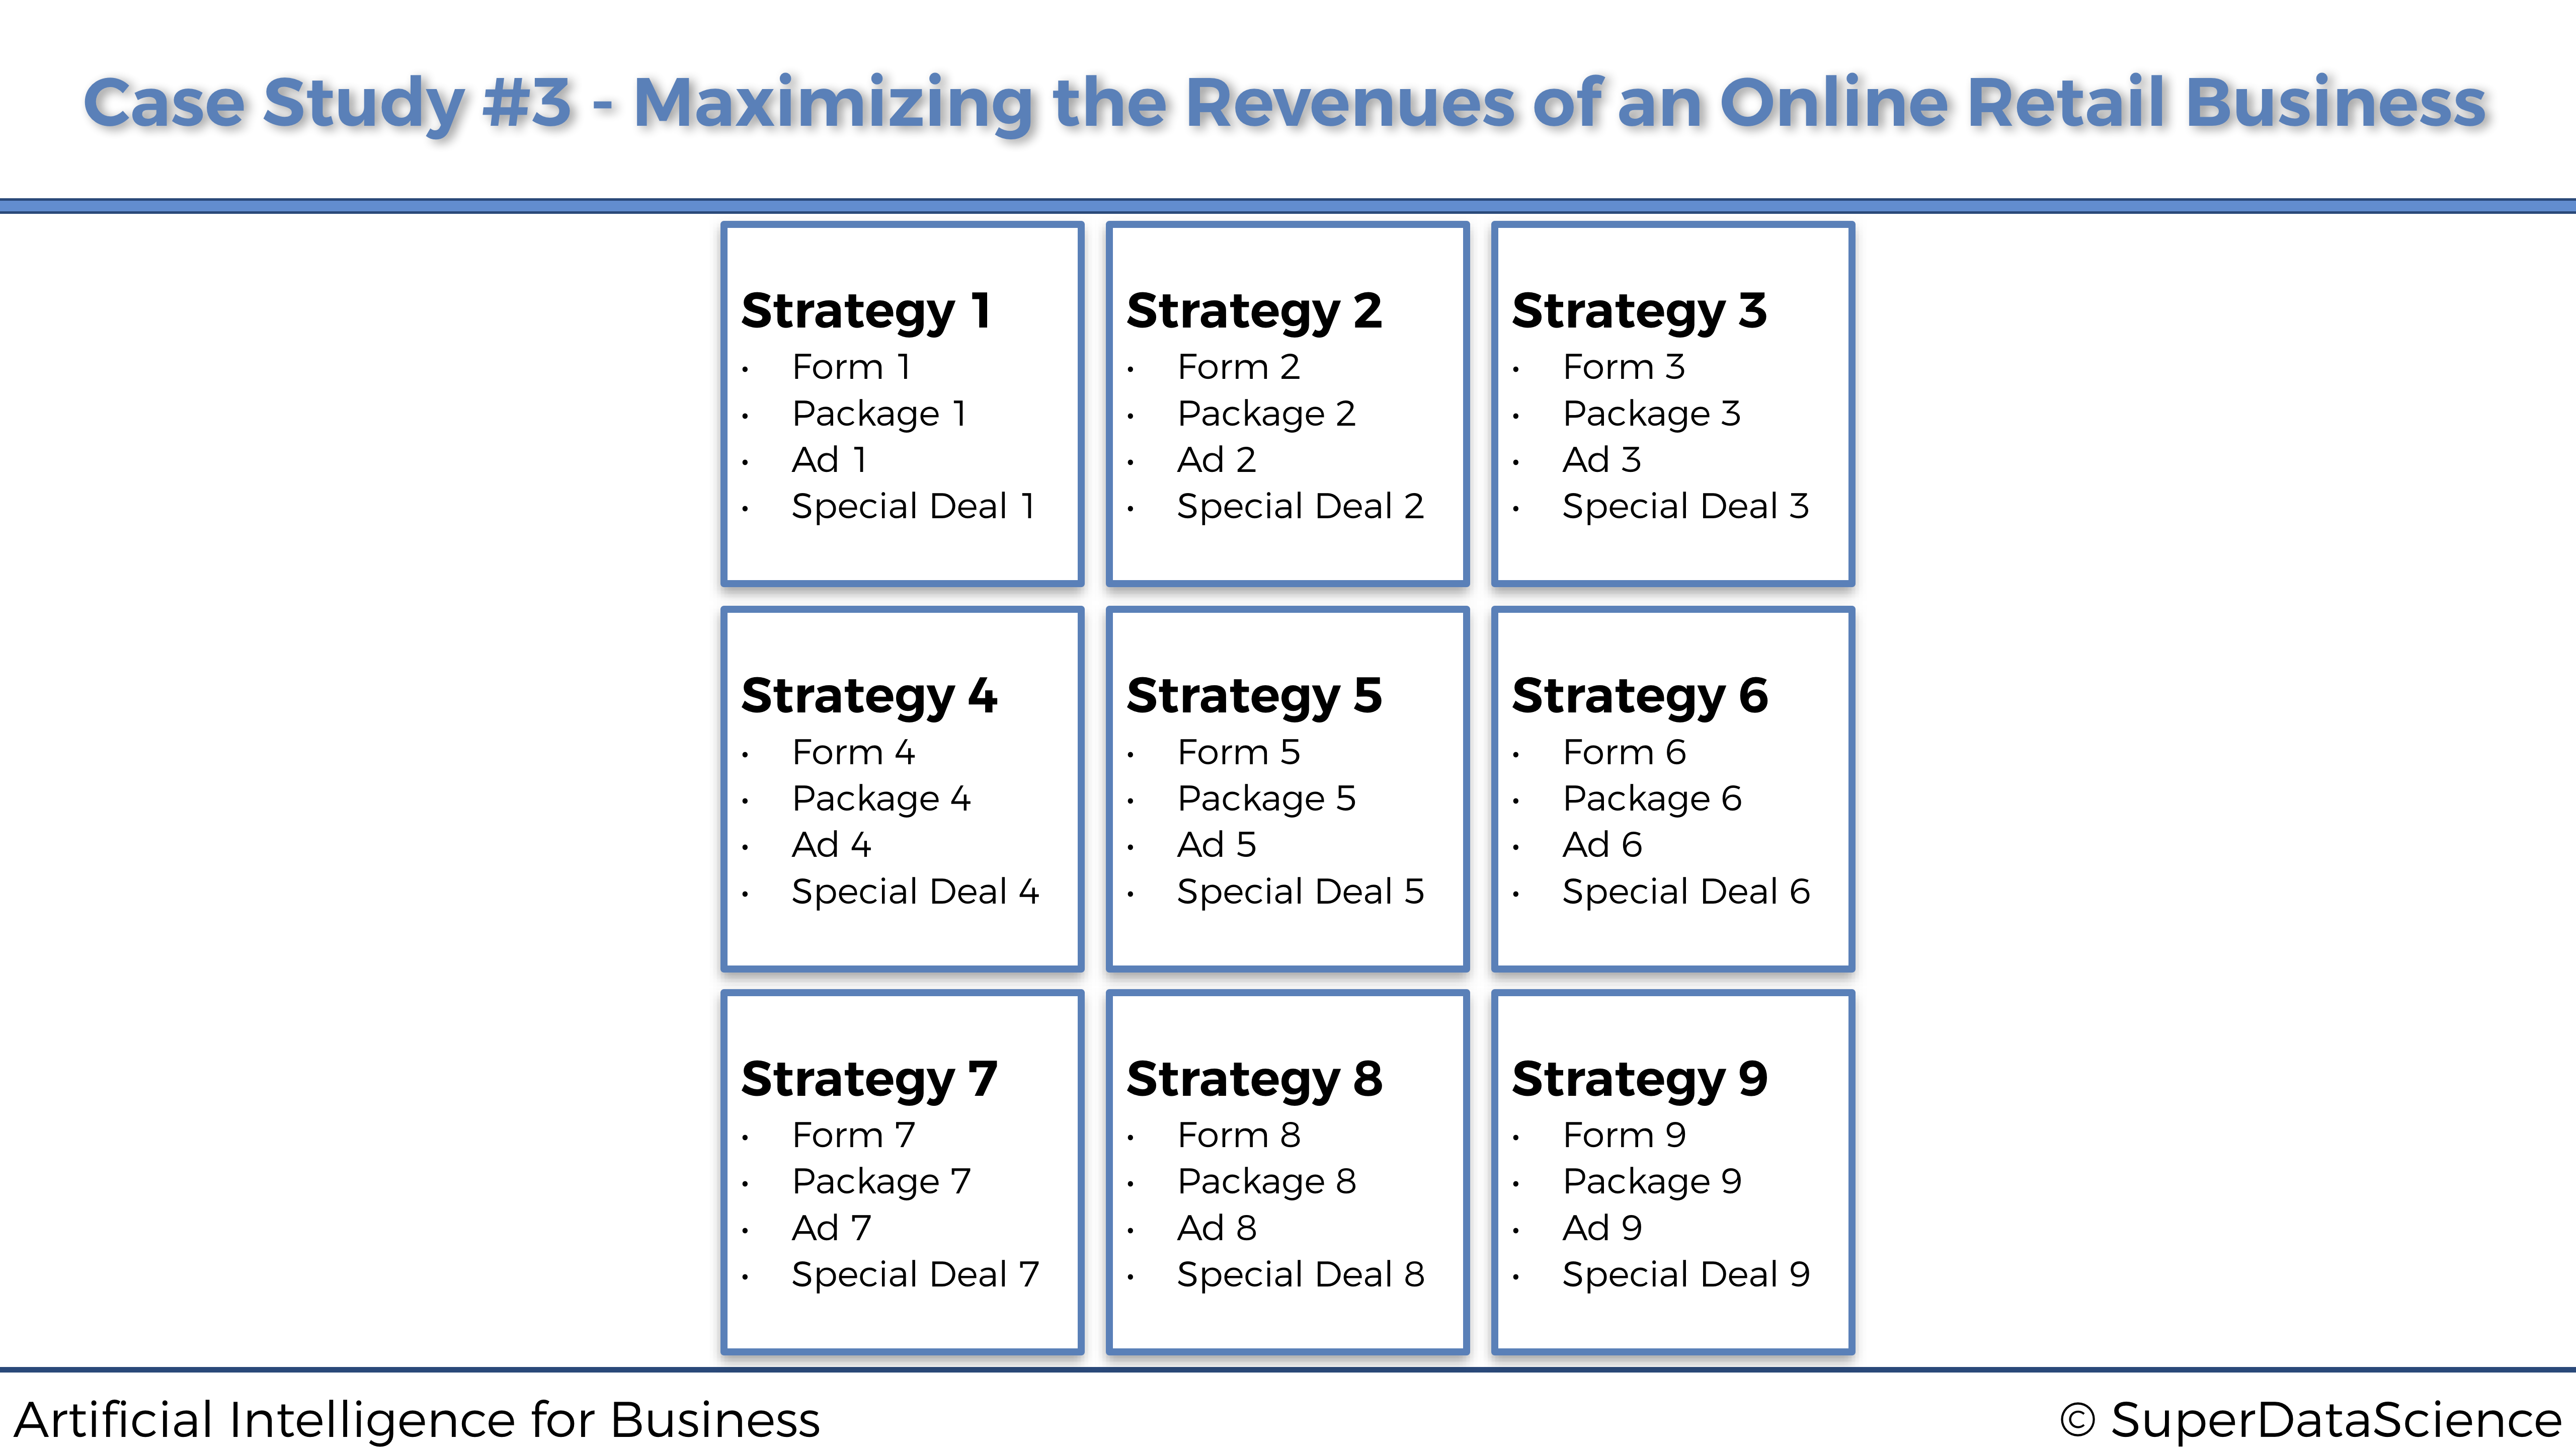
\includegraphics[scale=0.165]{Strategies_Slide.png}
        \end{center}
\end{figure}

\textbf{Simulation.}

In order to simulate this case study, we will assume these strategies have the following conversion rates:

\begin{figure}[!htbp]
        \begin{center}
            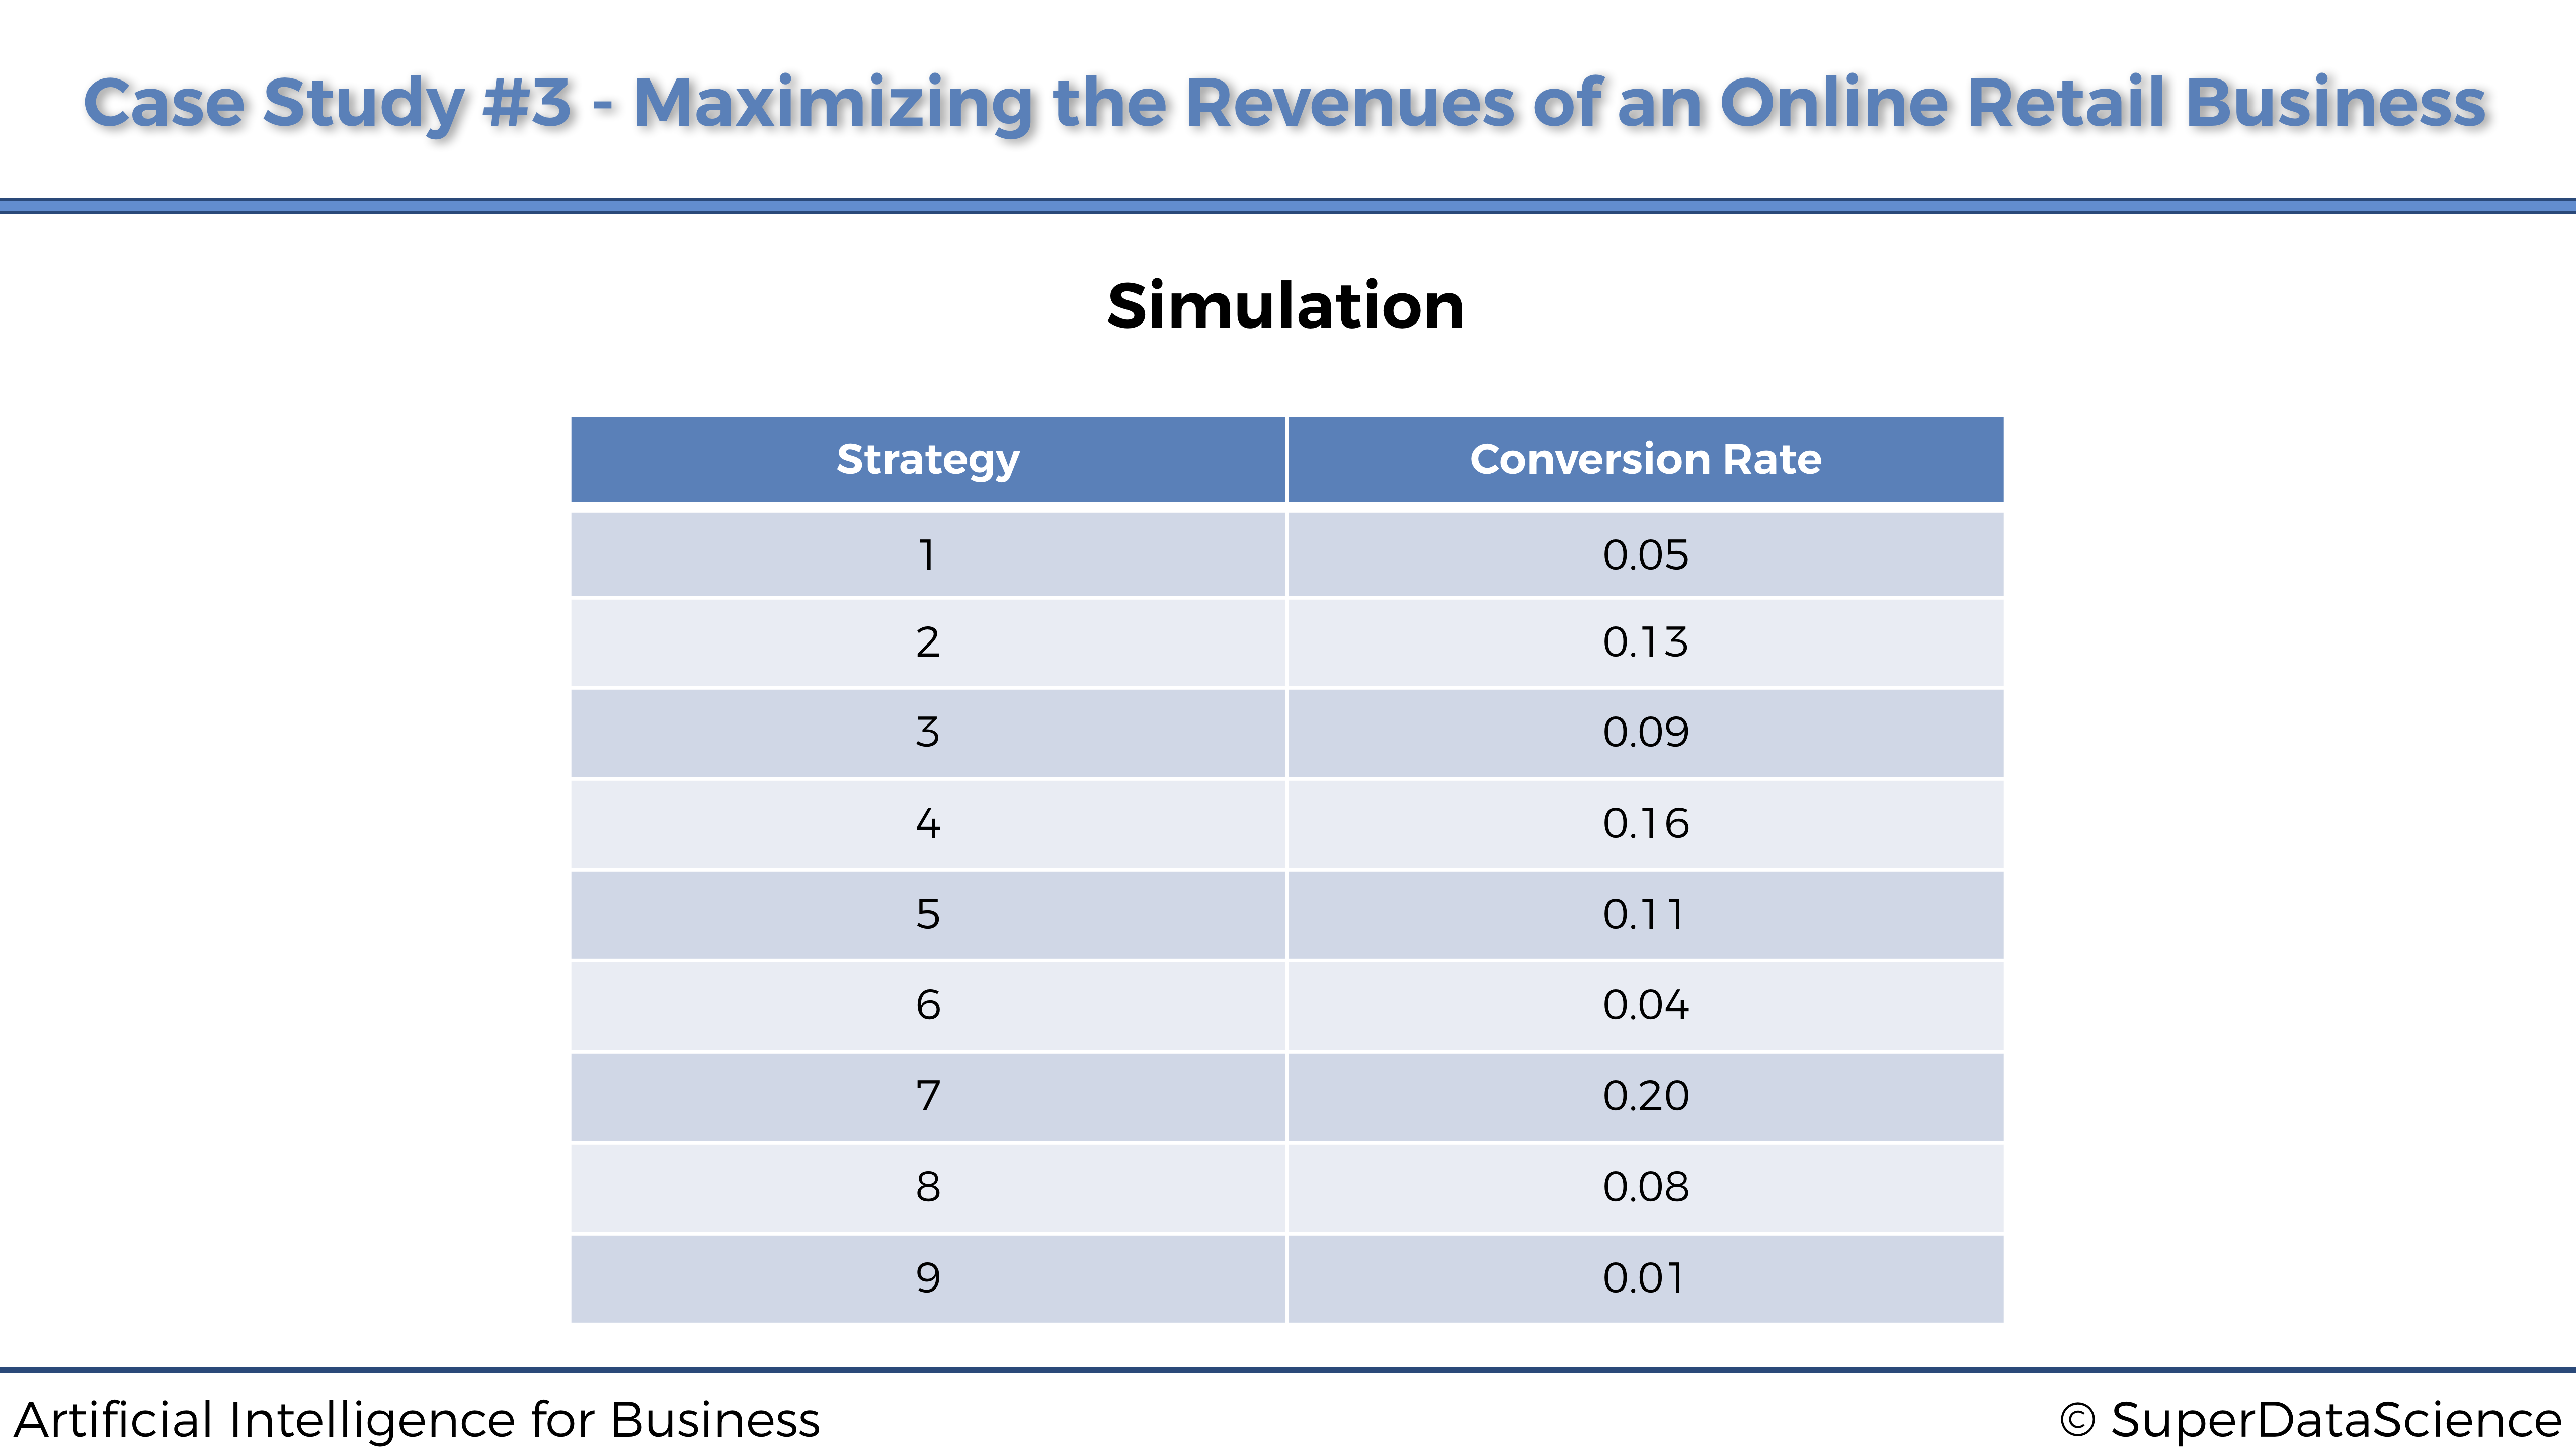
\includegraphics[scale=0.165]{Simulation_Slide.png}
        \end{center}
\end{figure}

However, please make sure to understand that in a real life situation we would have no idea of what would be these conversion rates. We only know them here for simulation purposes, just so that we can check in the end that our AI manages to figure out the best strategy, which according to the table above, is strategy number 7 (highest conversion rate).

\subsubsection{Environment to define}

Online Learning is a special branch of Artificial Intelligence, where there is not much need of defining the states and actions. Here, a state would simply be a specific customer onto whom we deploy a strategy, and the action would simply be the strategy selected. But you will see further in the AI algorithm that we don't have the states as inputs and the actions as outputs like in our two previous case studies, because this time we are not doing Q-Learning or Deep Q-Learning. Here we are doing online learning. However we do have to define the rewards, since again we will have to make a rewards matrix, where each row corresponds to a user being deployed a strategy, and each column corresponds to one of the 9 strategies. Therefore, since we will actually run this online learning experiment on 10,000 customers, this rewards matrix will have 10,000 rows and 9 columns. Then, each cell will get either a 0 if the customer doesn't subscribe to the premium plan after being approached by the selected strategy, and a 1 if the customer does subscribe after being approached by the selected strategy. And the values in the cell are exactly, the rewards.

Now a very important thing to understand is that the rewards matrix is only here for the simulation, and in real life we would have no such thing as a rewards matrix. We will just simulate 10,000 customers successively being approached by one of the 9 strategies, and thanks to the rewards matrix we will simulate the decision of the customer to subscribe yes or no to the premium plan. If the cell corresponding to a specific customer and a specific selected strategy has a 1, that will simulate a conversion by the customer to the premium plan, and if the cell has a 0, that will simulate a rejection. Here is below as an example the first rows of a simulated rewards matrix:

\begin{figure}[!htbp]
        \begin{center}
            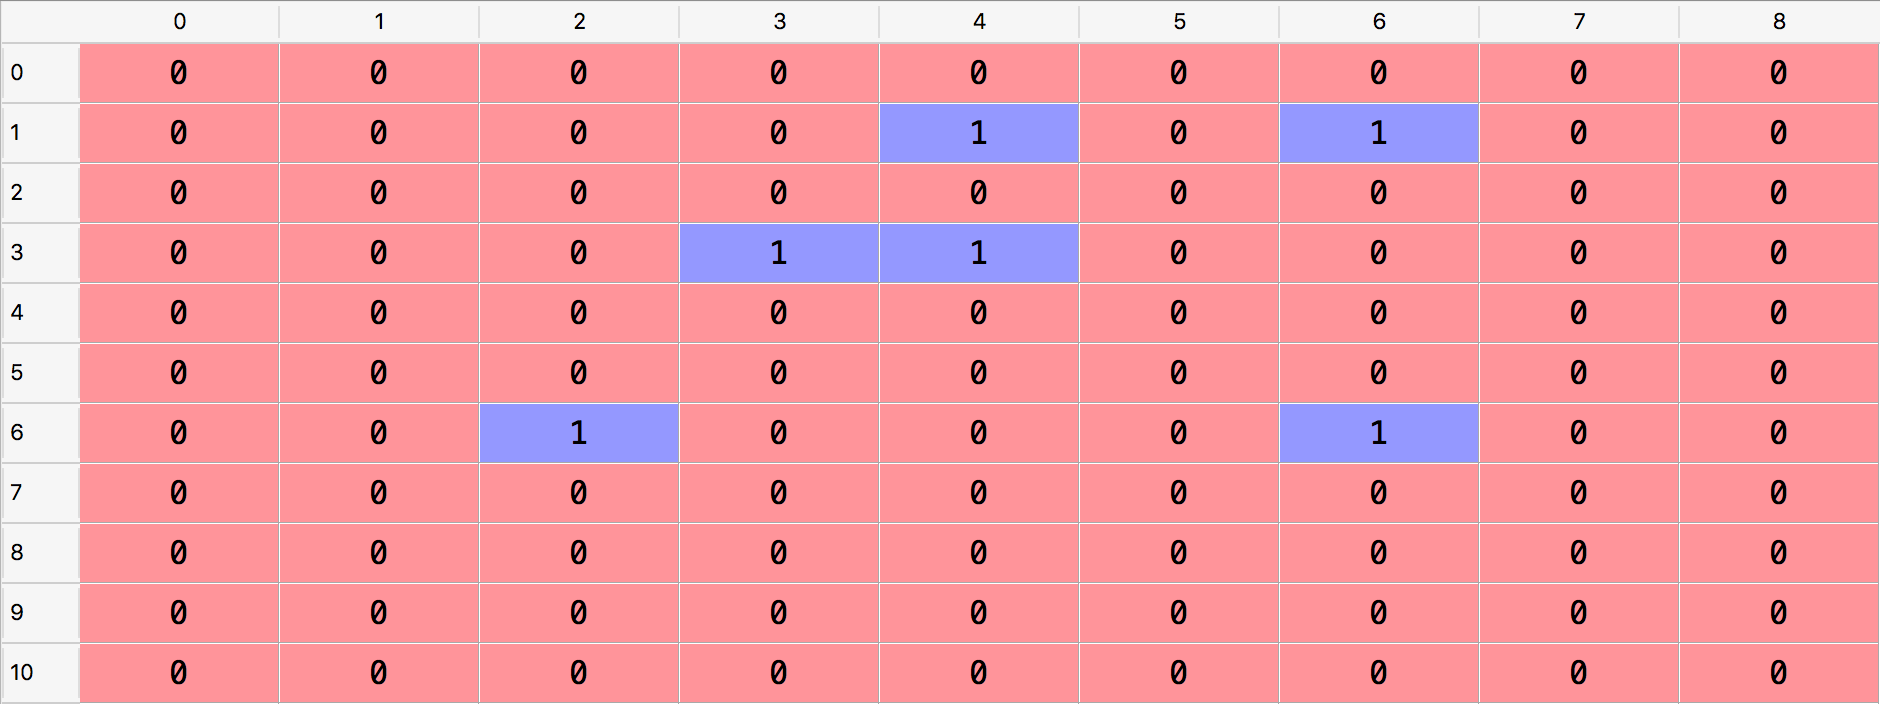
\includegraphics[scale=0.49]{Rewards_Matrix.png}
        \end{center}
\end{figure}

According to this simulation, all given in the above rewards matrix:

\begin{enumerate}
    \item The first customer (row of index 0) would not subscribe to the premium plan after being approached by any strategy.
    \item The second customer (row of index 1) would subscribe to the premium plan after being approached by strategy 5 or strategy 7 only.
    \item The third customer (row of index 2) would not subscribe to the premium plan after being approached by any strategy.
\end{enumerate}

Thompson Sampling will collect the feed-backs of whether or not each of these customers subscribe to the premium plan one after the other, and thanks to its powerful algorithm, will quickly figure out the strategy with the highest conversion rate, that is the best one to be deployed on the millions of customers, thus maximizing the company's income from this new revenue stream.

\subsection{AI Solution}

The AI solution that will figure out the best strategy is called ``Thompson Sampling''. It is by far the best model for that kind of problems in this Online Learning branch of Artificial Intelligence. To recap, each time a new customer connects to the online retail business website, that's a new round \(n\) and we select one of our 9 strategies to attempt a conversion (subscription to the premium plan). The goal is to select the best strategy at each round, over many rounds. Here is how Thompson Sampling will do that:

\textbf{For each round $n$, repeat, over 1000 rounds, the following three steps:}

\begin{enumerate}

    \item \textbf{Step 1.} For each strategy $i$, we take a random draw from the following distribution:
    \begin{equation*}
        \theta_i(n) \sim \beta(N_i^1(n)+1,N_i^0(n)+1)
    \end{equation*}
    where:
    \begin{equation*}
        \begin{cases}
            \textrm{$N_i^1(n)$ is the number of times the strategy $i$ has received a 1 reward up to round $n$,} \\
            \textrm{$N_i^0(n)$ is the number of times the strategy $i$ has received a 0 reward up to round $n$.}
        \end{cases}
    \end{equation*}
    
    \item \textbf{Step 2.} We select the strategy $s(n)$ that has the highest $\theta_i(n)$:
    \begin{equation*}
        s(n) = \underset{i\in\{1,...,9\}}{\textrm{argmax}}(\theta_i(n))
    \end{equation*}
    
    \item \textbf{Step 3.} We update $N_{s(n)}^1(n)$ and $N_{s(n)}^0(n)$ according to the following conditions:
    \begin{itemize}
        \item If the strategy selected $s(n)$ received a 1 reward:
        \begin{equation*}
            N_{s(n)}^1(n) := N_{s(n)}^1(n) + 1
        \end{equation*}
        \item If the strategy selected $s(n)$ received a 0 reward:
        \begin{equation*}
            N_{s(n)}^0(n) := N_{s(n)}^0(n) + 1
        \end{equation*}
    \end{itemize}

\end{enumerate}

\textbf{Intuition.} Each strategy has its own beta distribution. Over the rounds, the beta distribution of the strategy with the highest conversion rate will be progressively shifted to the right, and the beta distributions of the strategies with lower conversion rates will be progressively shifted to the left (Steps 1 and 3). Therefore, because of Step 2, the strategy with the highest conversion rate will be more and more selected. Below is a graph displaying three beta distributions of three strategies, that will help you visualize this:

\begin{figure}[!htbp]
        \begin{center}
            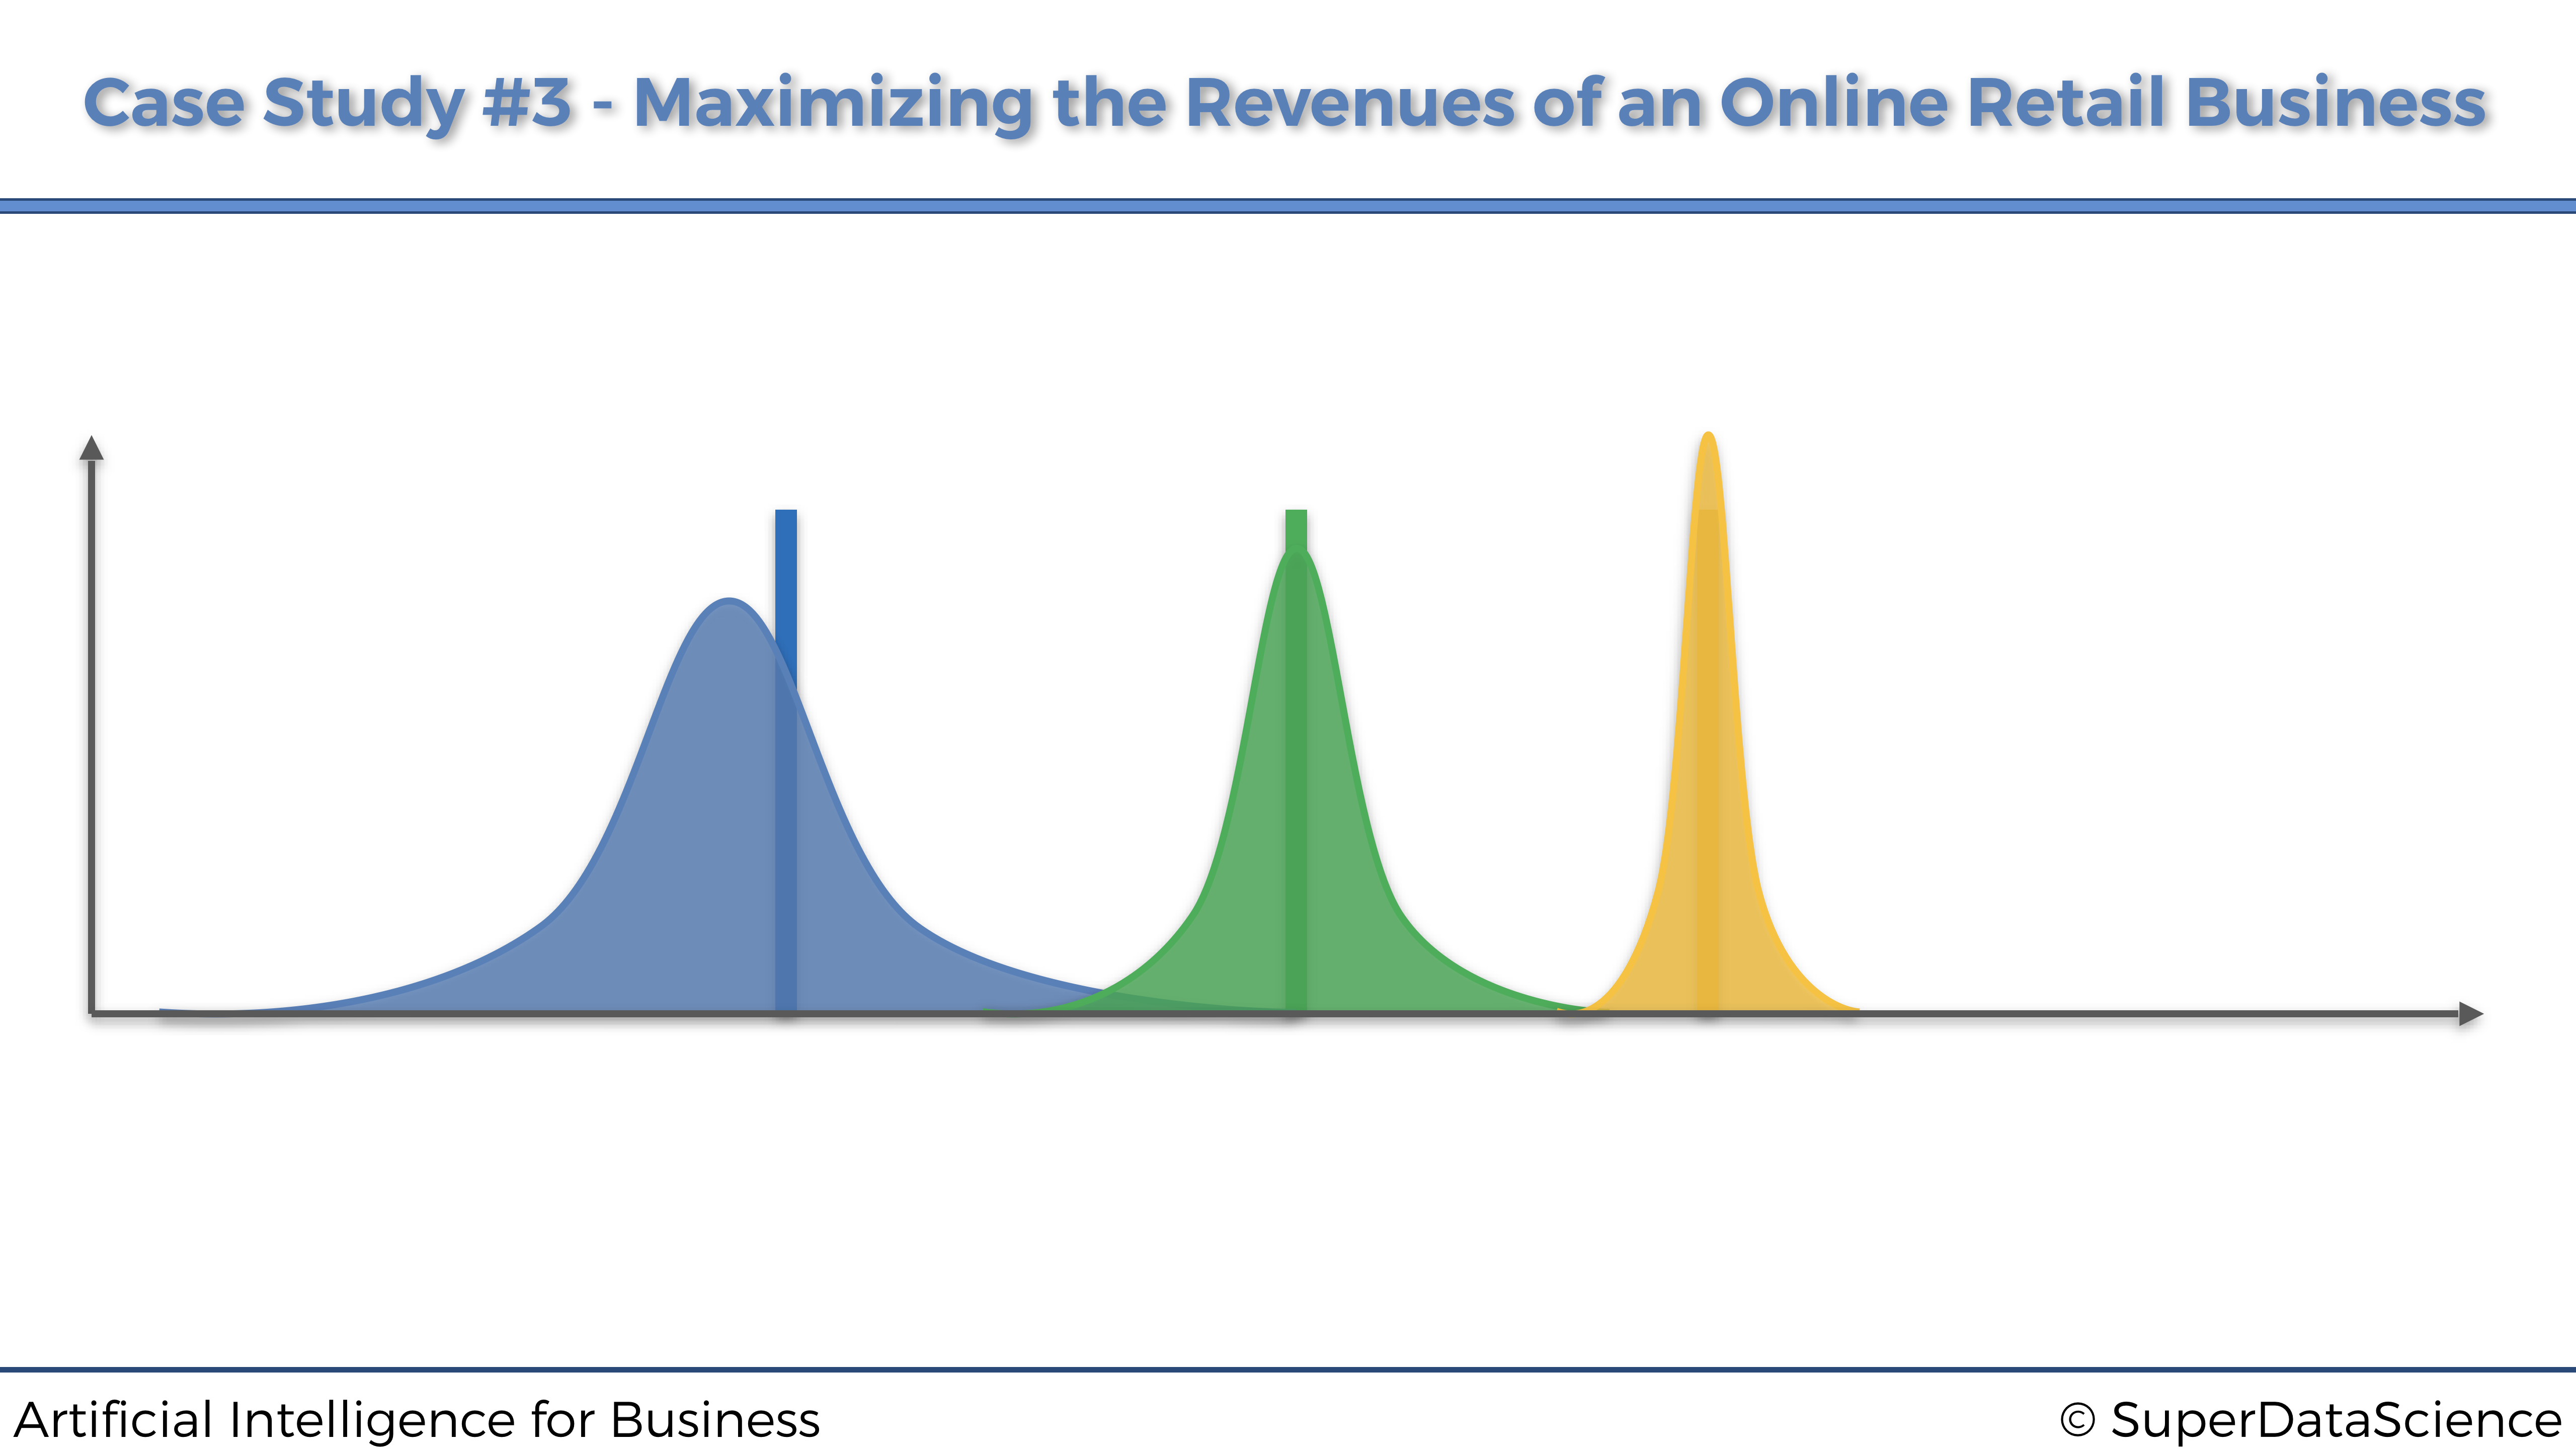
\includegraphics[scale=0.1]{Beta_Distribution_Slide.png}
        \end{center}
\end{figure}

\newpage

\subsection{Implementation}

Let's provide the whole implementation of Thompson Sampling for this specific case study, following the same simulation given above.

While implementing Thompson Sampling, we will also implement the Random Selection algorithm, which will simply select a random strategy at each round. This will be our benchmark to evaluate the performance of our Thompson Sampling model. Of course, Thompson Sampling and the Random Selection algorithm will be competing on the same simulation, that is on the same rewards matrix. And in the end, after the whole simulation is done, we will assess the performance of Thompson Sampling by computing the relative return, defined by the following formula:

\begin{equation*}
    \textrm{Relative Return} = \frac{\textrm{(Total Reward of Thompson Sampling)} - (\textrm{Total Reward of Random Selection})}{\textrm{Total Reward of Random Selection}} \times 100
\end{equation*}

We will also plot the histogram of selected ads, just to check that the strategy with the highest conversion rate (Strategy 7) was the one selected the most.

So if you are ready, here we go:

First, we import the required libraries and we set the parameters (\(N = 10000\) customers and \(d = 9\) strategies):

\begin{lstlisting}
# Artificial Intelligence for Business
# Maximizing the Revenues of an Online Retail Business with Thompson Sampling

# Importing the libraries
import numpy as np
import matplotlib.pyplot as plt
import random

# Setting the parameters
N = 10000
d = 9
\end{lstlisting}

Then, we create the simulation, by building the rewards matrix of 10000 rows corresponding to the customers, and 9 columns corresponding to the strategies. At each round and for each strategy, we draw a random number between 0 and 1, and if this random number is lower than the conversion rate of the strategy, the reward will be 1. Otherwise, it will be 0. That way we simulate the conversion rates listed above for our 9 strategies:

\begin{lstlisting}
# Creating the simulation
# conversion_rates = [0.1,0.2,0.3,0.4,0.5,0.6,0.7,0.8,0.9]
conversion_rates = [0.05,0.13,0.09,0.16,0.11,0.04,0.20,0.08,0.01]
X = np.array(np.zeros([N,d]))
for i in range(N):
    for j in range(d):
        if np.random.rand() <= conversion_rates[j]:
            X[i,j] = 1
\end{lstlisting}

Then, we will loop over the 10000 rows (or rounds) of this rewards matrix, and at each round we will get two separate strategy selections: one from the Random Selection algorithm, and one from Thompson Sampling. We keep track of the strategies selected by each of these two algorithms, and we compute the total reward accumulated over the rounds by each of them. Thompson Sampling is implemented following exactly the Steps 1, 2 and 3 provided above:

\begin{lstlisting}
# Implementing a Random Strategy and Thompson Sampling
strategies_selected_rs = []
strategies_selected_ts = []
total_reward_rs = 0
total_reward_ts = 0
numbers_of_rewards_1 = [0] * d
numbers_of_rewards_0 = [0] * d
for n in range(0, N):
    # Random Strategy
    strategy_rs = random.randrange(d)
    strategies_selected_rs.append(strategy_rs)
    reward_rs = X[n, strategy_rs]
    total_reward_rs = total_reward_rs + reward_rs
    # Thompson Sampling
    strategy_ts = 0
    max_random = 0
    for i in range(0, d):
        random_beta = random.betavariate(numbers_of_rewards_1[i] + 1,
                                         numbers_of_rewards_0[i] + 1)
        if random_beta > max_random:
            max_random = random_beta
            strategy_ts = i
    reward_ts = X[n, strategy_ts]
    if reward_ts == 1:
        numbers_of_rewards_1[strategy_ts] = numbers_of_rewards_1[strategy_ts] + 1
    else:
        numbers_of_rewards_0[strategy_ts] = numbers_of_rewards_0[strategy_ts] + 1
    strategies_selected_ts.append(strategy_ts)
    total_reward_ts = total_reward_ts + reward_ts
\end{lstlisting}

Then we compute the final score, which is the relative return of Thompson Sampling with respect to our benchmark that is the Random Selection:

\begin{lstlisting}
# Computing the Relative Return
relative_return = (total_reward_ts - total_reward_rs) / total_reward_rs * 100
print("Relative Return: {:.0f} %".format(relative_return))
\end{lstlisting}

And buckle up, by executing this code we obtain a final relative return, of\ldots{}:

\begin{equation*}
    \textrm{Relative Return} = 91 \ \% \ !
\end{equation*}

In other words, Thompson Sampling almost doubled the performance of our Random Selection benchmark.

\newpage

And finally, we plot the Histogram of the selected strategies, to check that indeed Strategy 7 (of index 6) was the one most selected, since it is the one having the highest conversion rate:

\begin{lstlisting}
# Plotting the Histogram of Selections
plt.hist(strategies_selected_ts)
plt.title('Histogram of Selections')
plt.xlabel('Strategy')
plt.ylabel('Number of times the strategy was selected')
plt.show()
\end{lstlisting}

By executing this final code, we obtain the following histogram:

\begin{figure}[!htbp]
        \begin{center}
            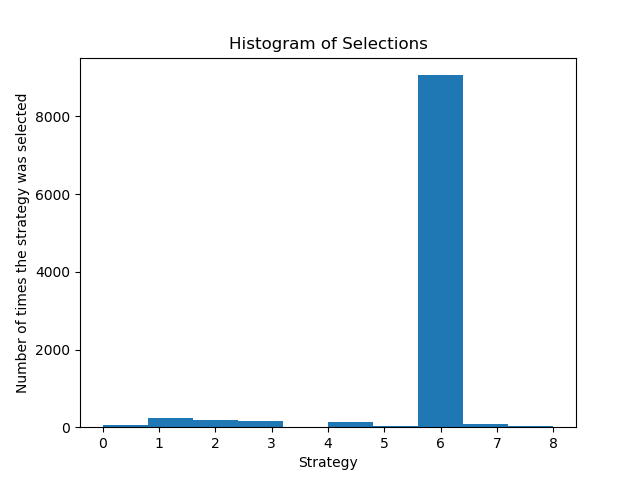
\includegraphics[scale=0.8]{Histogram.png}
        \end{center}
\end{figure}

And indeed, it is well the strategy of index 6, that is Strategy 7, that was, by far, selected the most. Thompson Sampling was quickly able to identify it. And in fact, if we re-run the same code but with only 1000 customers, we realize that Thompson Sampling is still able to identify Strategy 7 as the best one.

Accordingly, Thompson Sampling surely did an amazing job for this Online Retail Business. Because not only it was able to identify the best strategy quickly in a few number of rounds, that is with a few customers, which saved a lot on the advertising and operating related costs. But also because of course, it was able to clearly figure out the strategy with the highest conversion rate. And indeed, if this Online Retail Business has 100 million customers, and if the premium plan has a price of \$ 100 per year, then deploying this best strategy that has a conversion rate of 20 \% would lead to generate an extra revenue of\ldots{}:

\begin{equation*}
    \textrm{Extra Revenues generated} = 100000000 \times 0.2 \times 100 = \textrm{\$ $2$ Billion !!}
\end{equation*}

In other words, Thompson Sampling clearly and quickly maximized the revenues of this online retail business, while also saving a lot on the costs, therefore maximizing as well the profitability of the business.

\textbf{Regret Curve.}

The regret curve of a model (Random Strategy or Thompson Sampling) is the plot of the difference between the best strategy and the deployed model, with respect to the rounds.

The best strategy is computed by simply getting, at each round, the maximum of the accumulated rewards over all the different strategies. Therefore in our implementation, we will get the best strategy the following way:

\begin{lstlisting}
rewards_strategies = [0] * d
for n in range(0, N):
    # Best Strategy
    for i in range(0, d):
        rewards_strategies[i] = rewards_strategies[i] + X[n, i]
    total_reward_bs = max(rewards_strategies)
\end{lstlisting}

Then, the regret of Thompson Sampling is simply computed as the difference between the best strategy and the Thompson Sampling model:

\begin{lstlisting}
# Regret of Thompson Sampling
strategies_selected_ts = []
total_reward_ts = 0
total_reward_bs = 0
numbers_of_rewards_1 = [0] * d
numbers_of_rewards_0 = [0] * d
rewards_strategies = [0] * d
regret = []
for n in range(0, N):
    # Thompson Sampling
    strategy_ts = 0
    max_random = 0
    for i in range(0, d):
        random_beta = random.betavariate(numbers_of_rewards_1[i] + 1,
                                         numbers_of_rewards_0[i] + 1)
        if random_beta > max_random:
            max_random = random_beta
            strategy_ts = i
    reward_ts = X[n, strategy_ts]
    if reward_ts == 1:
        numbers_of_rewards_1[strategy_ts] = numbers_of_rewards_1[strategy_ts] + 1
    else:
        numbers_of_rewards_0[strategy_ts] = numbers_of_rewards_0[strategy_ts] + 1
    strategies_selected_ts.append(strategy_ts)
    total_reward_ts = total_reward_ts + reward_ts
    # Best Strategy
    for i in range(0, d):
        rewards_strategies[i] = rewards_strategies[i] + X[n, i]
    total_reward_bs = max(rewards_strategies)
    # Regret
    regret.append(total_reward_bs - total_reward_ts)
\end{lstlisting}

And same, the regret of the Random Strategy is simply computed as the difference between the best strategy and the random selection algorithm:

\begin{lstlisting}
# Regret of the Random Strategy
strategies_selected_rs = []
total_reward_rs = 0
total_reward_bs = 0
numbers_of_rewards_1 = [0] * d
numbers_of_rewards_0 = [0] * d
rewards_strategies = [0] * d
regret = []
for n in range(0, N):
    # Random Strategy
    strategy_rs = random.randrange(d)
    strategies_selected_rs.append(strategy_rs)
    reward_rs = X[n, strategy_rs]
    total_reward_rs = total_reward_rs + reward_rs
    # Best Strategy
    for i in range(0, d):
        rewards_strategies[i] = rewards_strategies[i] + X[n, i]
    total_reward_bs = max(rewards_strategies)
    # Regret
    regret.append(total_reward_bs - total_reward_rs)
\end{lstlisting}

And finally of course, we plot the regret over the rounds with this simple code (we don't have to specify the x-coordinates in the plt.plot() function because the rounds are already indexes from 0 to N):

\begin{lstlisting}
# Plotting the Regret Curve
plt.plot(regret)
plt.title('Regret Curve')
plt.xlabel('Round')
plt.ylabel('Regret')
plt.show()
\end{lstlisting}

Let's look at the results in the next page, for both the Random Strategy and Thompson Sampling.

\newpage

If we plot the Regret Curve of the Random Strategy, we thus obtain the following:

\begin{figure}[!htbp]
        \begin{center}
            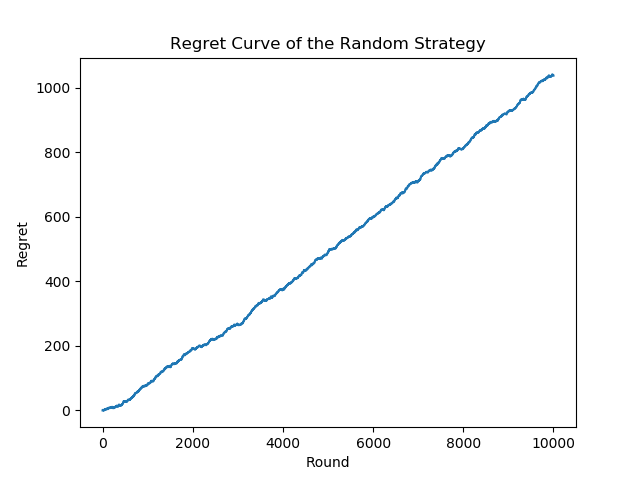
\includegraphics[scale=1]{Regret_Curve_Random_Strategy.png}
        \end{center}
\end{figure}

And of course, we observe absolutely no convergence of the Random Strategy towards the Best Strategy.

\newpage

However if now we plot the Regret Curve of the Thompson Sampling model, we get the following beautiful curve:

\begin{figure}[!htbp]
        \begin{center}
            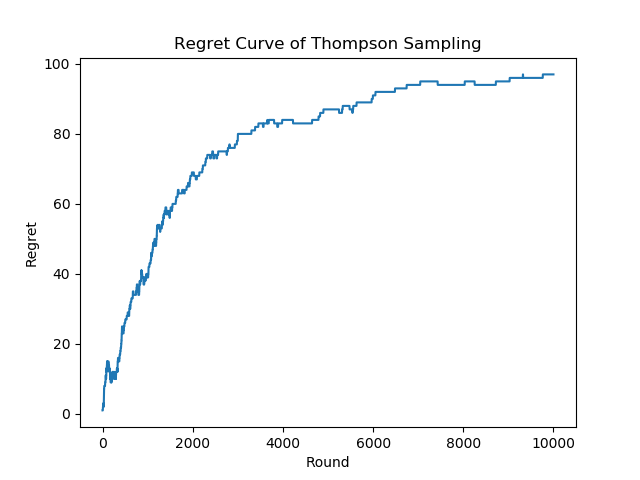
\includegraphics[scale=1]{Regret_Curve_Thompson_Sampling.png}
        \end{center}
\end{figure}

And obviously, Thompson Sampling is converging very well towards the best strategy.

\newpage

Eventually, here is the final code including that Regret Curve of Thompson Sampling:

\begin{lstlisting}
# Thompson Sampling

# Importing the libraries
import numpy as np
import matplotlib.pyplot as plt
import random

# Setting the parameters
N = 10000
d = 9

# Creating the simulation
# conversion_rates = [0.1,0.2,0.3,0.4,0.5,0.6,0.7,0.8,0.9]
conversion_rates = [0.05,0.13,0.09,0.16,0.11,0.04,0.20,0.08,0.01]
X = np.array(np.zeros([N,d]))
for i in range(N):
    for j in range(d):
        if np.random.rand() <= conversion_rates[j]:
            X[i,j] = 1

# Implementing a Random Strategy and Thompson Sampling with Regret Curve
strategies_selected_rs = []
strategies_selected_ts = []
total_reward_rs = 0
total_reward_ts = 0
total_reward_bs = 0
numbers_of_rewards_1 = [0] * d
numbers_of_rewards_0 = [0] * d
rewards_strategies = [0] * d
regret = []
for n in range(0, N):
    # Random Strategy
    strategy_rs = random.randrange(d)
    strategies_selected_rs.append(strategy_rs)
    reward_rs = X[n, strategy_rs]
    total_reward_rs = total_reward_rs + reward_rs
    # Thompson Sampling
    strategy_ts = 0
    max_random = 0
    for i in range(0, d):
        random_beta = random.betavariate(numbers_of_rewards_1[i] + 1,
                                         numbers_of_rewards_0[i] + 1)
        if random_beta > max_random:
            max_random = random_beta
            strategy_ts = i
    reward_ts = X[n, strategy_ts]
    if reward_ts == 1:
        numbers_of_rewards_1[strategy_ts] = numbers_of_rewards_1[strategy_ts] + 1
    else:
        numbers_of_rewards_0[strategy_ts] = numbers_of_rewards_0[strategy_ts] + 1
    strategies_selected_ts.append(strategy_ts)
    total_reward_ts = total_reward_ts + reward_ts
    # Best Strategy
    for i in range(0, d):
        rewards_strategies[i] = rewards_strategies[i] + X[n, i]
    total_reward_bs = max(rewards_strategies)
    # Regret
    regret.append(total_reward_bs - total_reward_ts)

# Computing the Absolute and Relative Return
absolute_return = total_reward_ts - total_reward_rs
relative_return = (total_reward_ts - total_reward_rs) / total_reward_rs * 100
print("Absolute Return: {:.0f} $".format(absolute_return))
print("Relative Return: {:.0f} %".format(relative_return))

# Plotting the Histogram of Selections
plt.hist(strategies_selected_ts)
plt.title('Histogram of Selections')
plt.xlabel('Strategy')
plt.ylabel('Number of times the strategy was selected')
plt.show()
plt.close()

# Plotting the Regret Curve
plt.plot(regret)
plt.title('Regret Curve')
plt.xlabel('Round')
plt.ylabel('Regret')
plt.show()

\end{lstlisting}

\hypertarget{conclusion}{%
\chapter{Conclusion}\label{conclusion}}

Thank you so much again for joining this course, and congratulations for completing it! We highly recommend that you keep this book close to you whenever you are building an AI to solve a business problem. Or at least, try to keep the general AI Framework. On our side, it was our pleasure making this course, and writing this book. Don't hesitate to leave a review in the course if you wish. Until then, enjoy AI for Business!

\hypertarget{annex-1-artificial-neural-networks}{%
\chapter{Annex 1: Artificial Neural Networks}\label{annex-1-artificial-neural-networks}}

In this annex part you will find all the intuition and theory of Artificial Neural Networks, which are at the heart of the Deep Q-Learning model we build in Part 2 - Minimizing the Costs. Here is the plan of attack to study Artificial Neural Networks:

\begin{enumerate}
    \item The Neuron
    \item The Activation Function
    \item How do Neural Networks work?
    \item How do Neural Networks learn?
    \item Forward-Propagation and Back-Propagation
    \item Gradient Descent
    \item Batch Gradient Descent and Stochastic Gradient Descent
\end{enumerate}

\subsection{The Neuron}

The neuron is the basic building block of Artificial Neural Networks. In the images below are actual real life neurons which have been smeared onto a glass, colored a little bit and observed through a microscope:

\begin{figure}[!htbp]
        \begin{center}
            \includegraphics[scale=0.18]{ANN_1.png}
        \end{center}
\end{figure}

As we can see, they have the structure of a body with lots of different branches coming out of them. But the question is: How can we recreate that in a machine? Indeed, we really need to recreate it in a machine since the whole purpose of Deep Learning is to mimic how the human brain works, in the hope that by doing so we are going to create something amazing: a powerful infrastructure for machines to be able to learn.

Why do we hope for that? Because the human brain just happens to be one of the most powerful learning tools on the planet. So we just hope that if we recreate it then we will have something as awesome as that. So our challenge right now, that is our very first step to creating artificial neural networks, is to recreate a neuron.

So how do we do it? Well, first of all let's have a closer look at what a neuron actually is. The image below was first created by a Spanish neuroscientist and Chagga Ramon Yi Kajal in 1899:

\begin{figure}[!htbp]
        \begin{center}
            \includegraphics[scale=0.16]{ANN_2.png}
        \end{center}
\end{figure}

This neuroscientist dyed in neurons in actual brain tissue, and looked at them under a microscope. While he was looking at them he actually drew what he saw, which is exactly what we see on the above image. Today technology has advanced quite a lot allowing us to see neurons much closer in more detail so that we can actually draw what it looks like diagrammatically.

\begin{figure}[!htbp]
        \begin{center}
            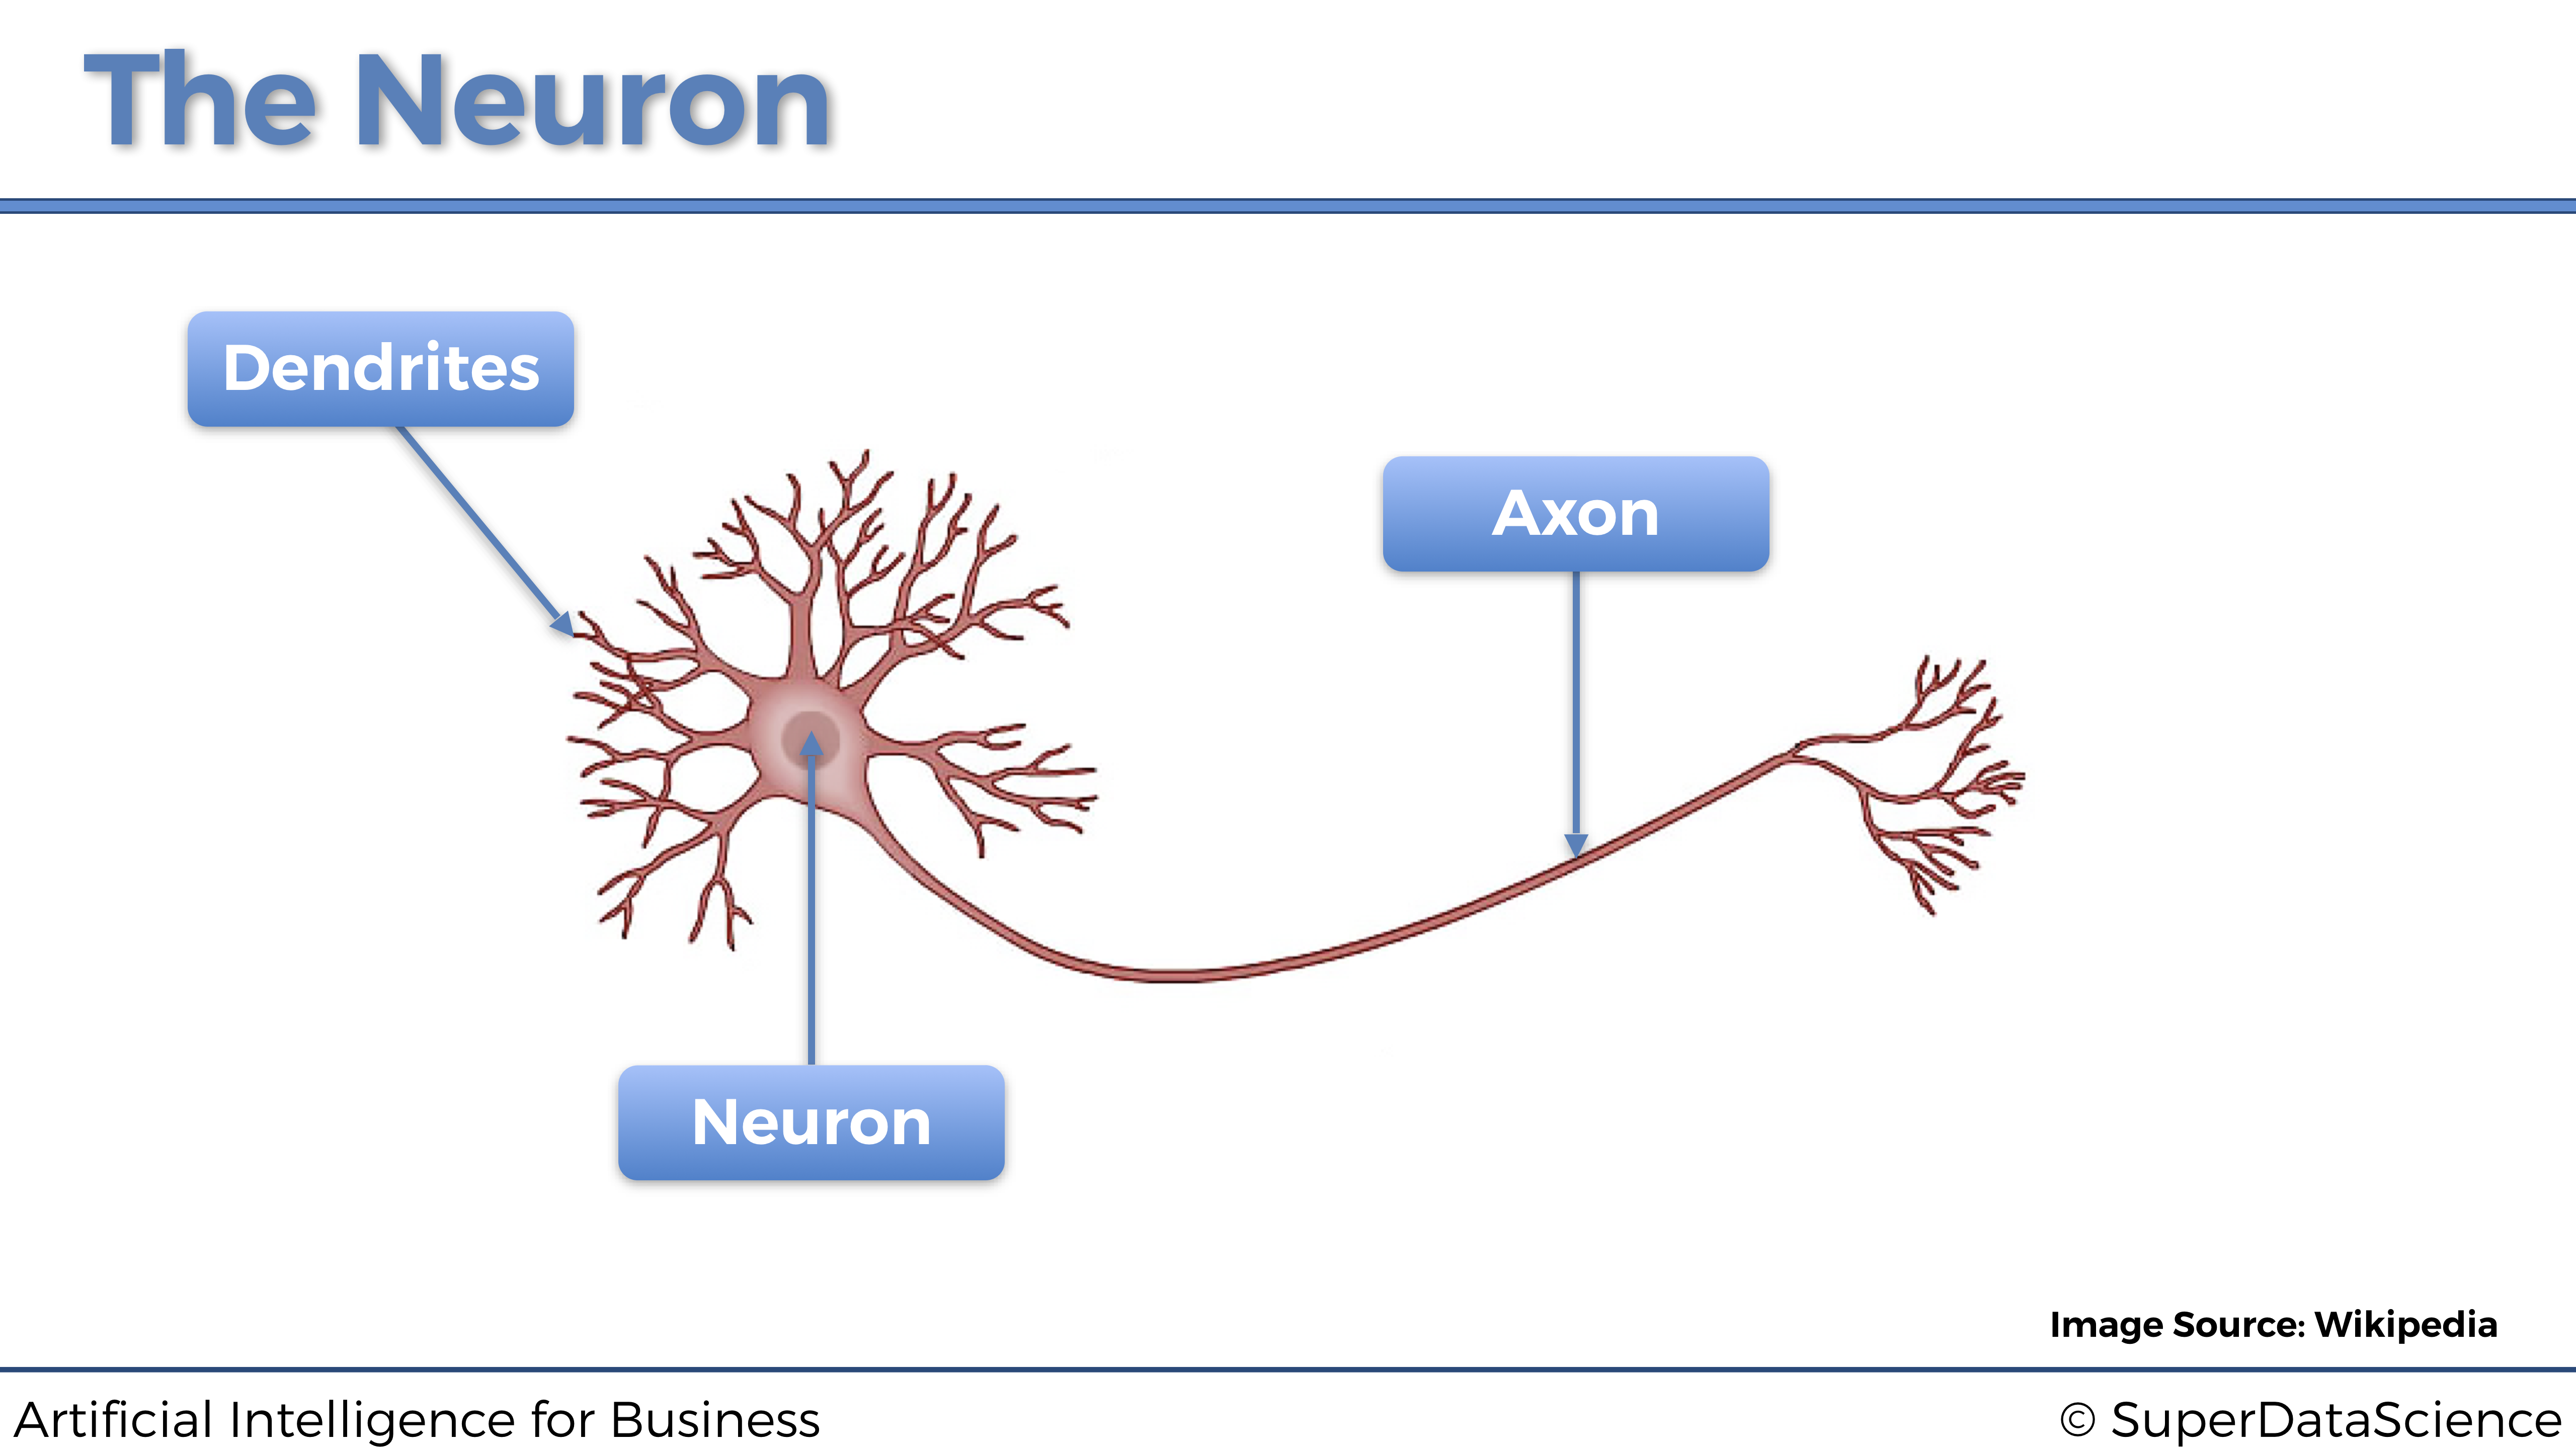
\includegraphics[scale=0.16]{ANN_3.png}
        \end{center}
\end{figure}

Above is a neuron. This neuron exchanges signals between its neighbour neurons. The dendrites are the receivers of the signal and the axon is the transmitter of the signal. Here is an image of how it all works conceptually:

\begin{figure}[!htbp]
        \begin{center}
            \includegraphics[scale=0.16]{ANN_4.png}
        \end{center}
\end{figure}

We can see that the dendrites of the neuron are connected to the axons of other neurons above it. Then the signal travels down its axon and passes on to the dendrites of the next neuron. That is how they are connected and how a neuron works. Thus now is the time to move from neuroscience to technology.

Here is how a neuron is represented inside an Artificial Neural Network:

\begin{figure}[!htbp]
        \begin{center}
            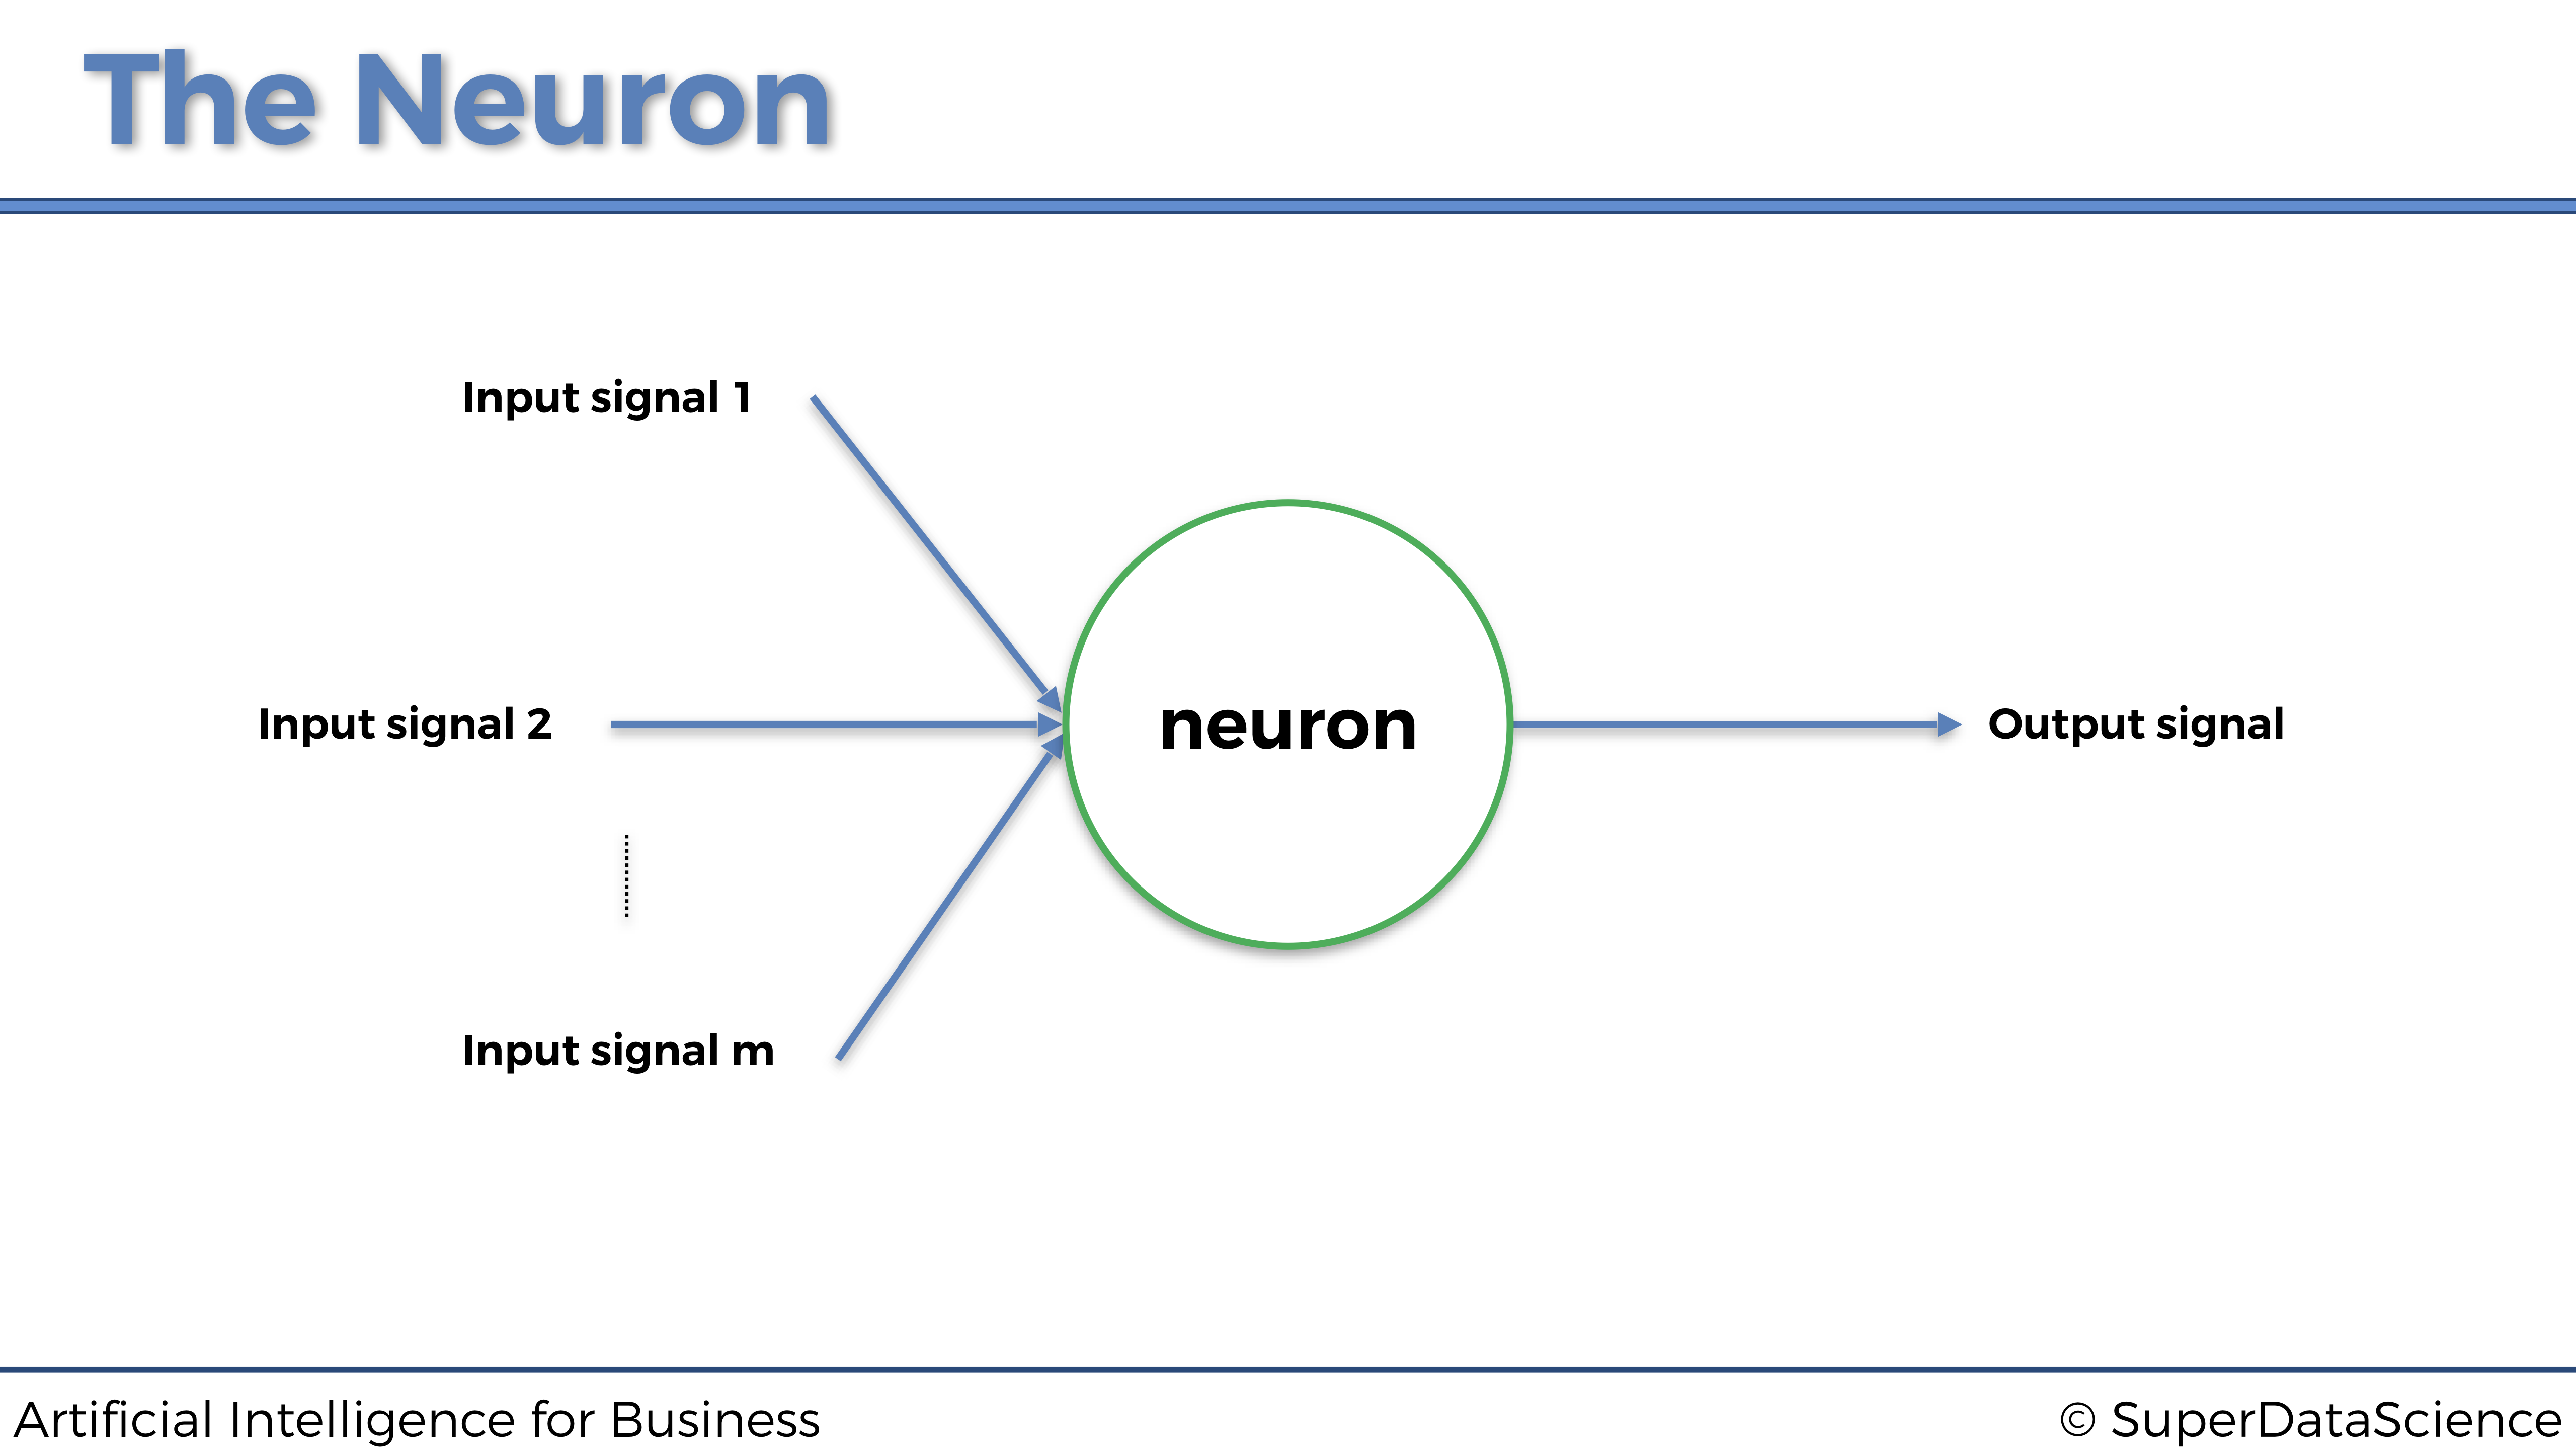
\includegraphics[scale=0.175]{ANN_5.png}
        \end{center}
\end{figure}

Just as a human neuron, it gets some input signals and it has an output signal. The blue arrow connecting the input signals to the neuron, and the neuron to the output signal, are like the synapses in the human neuron. But here in the machine neuron, what are exactly going to be these input and output signals? Well, the input signals are going to be the scaled independent variables composing the states of the environment, which remember in the case study are the temperature of the server, the number of users and the rate of data transmission, and the output signal will be the output values, which in the Deep Q-Learning model are always the Q-Values. Hence we get the general representation of a neuron for machines:

\begin{figure}[!htbp]
        \begin{center}
            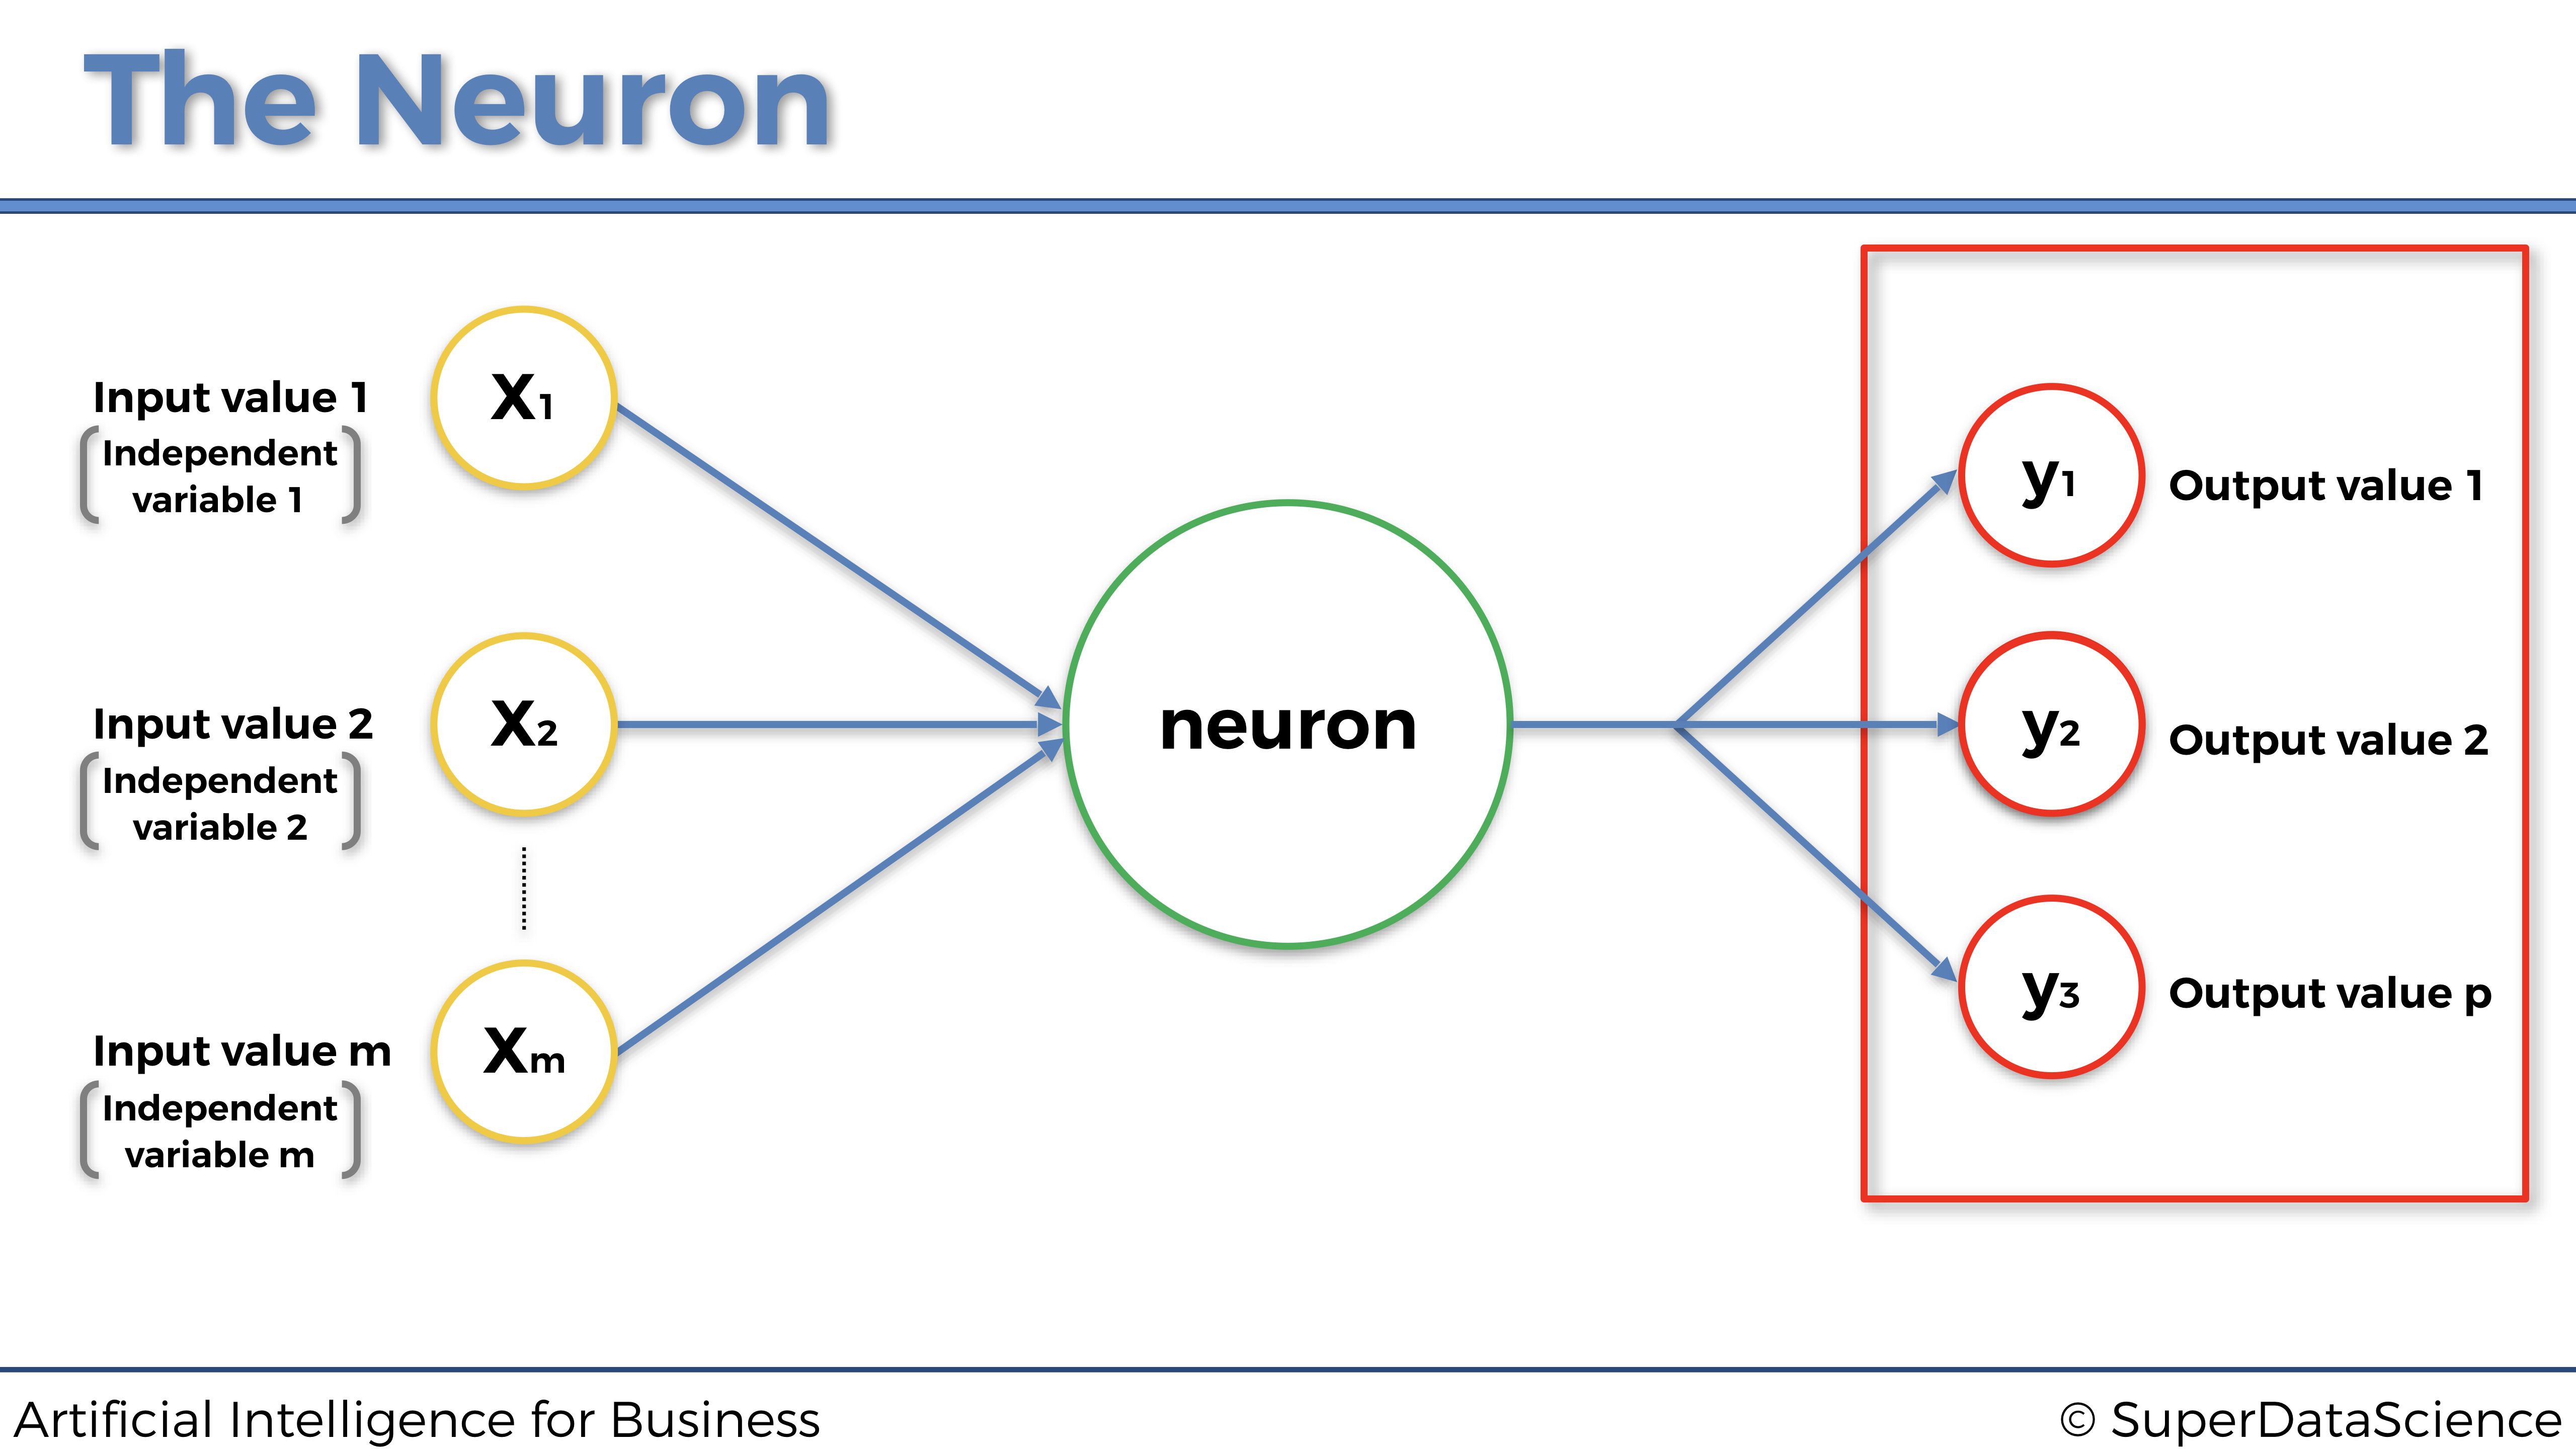
\includegraphics[scale=0.15]{ANN_7.png}
        \end{center}
\end{figure}

And now to finish with the neuron, let's add the last missing elements in this representation, but also the most important ones: the weights. Each synapse (blue arrow) will be attributed a weight. The larger is the weight, the stronger the signal will be through the synapse. And what is fundamental to understand is that, these weights, will be what the machine will update and update over time to improve the predictions. Let's represent them on the previous graphic, to make sure we all visualize them well:

\begin{figure}[!htbp]
        \begin{center}
            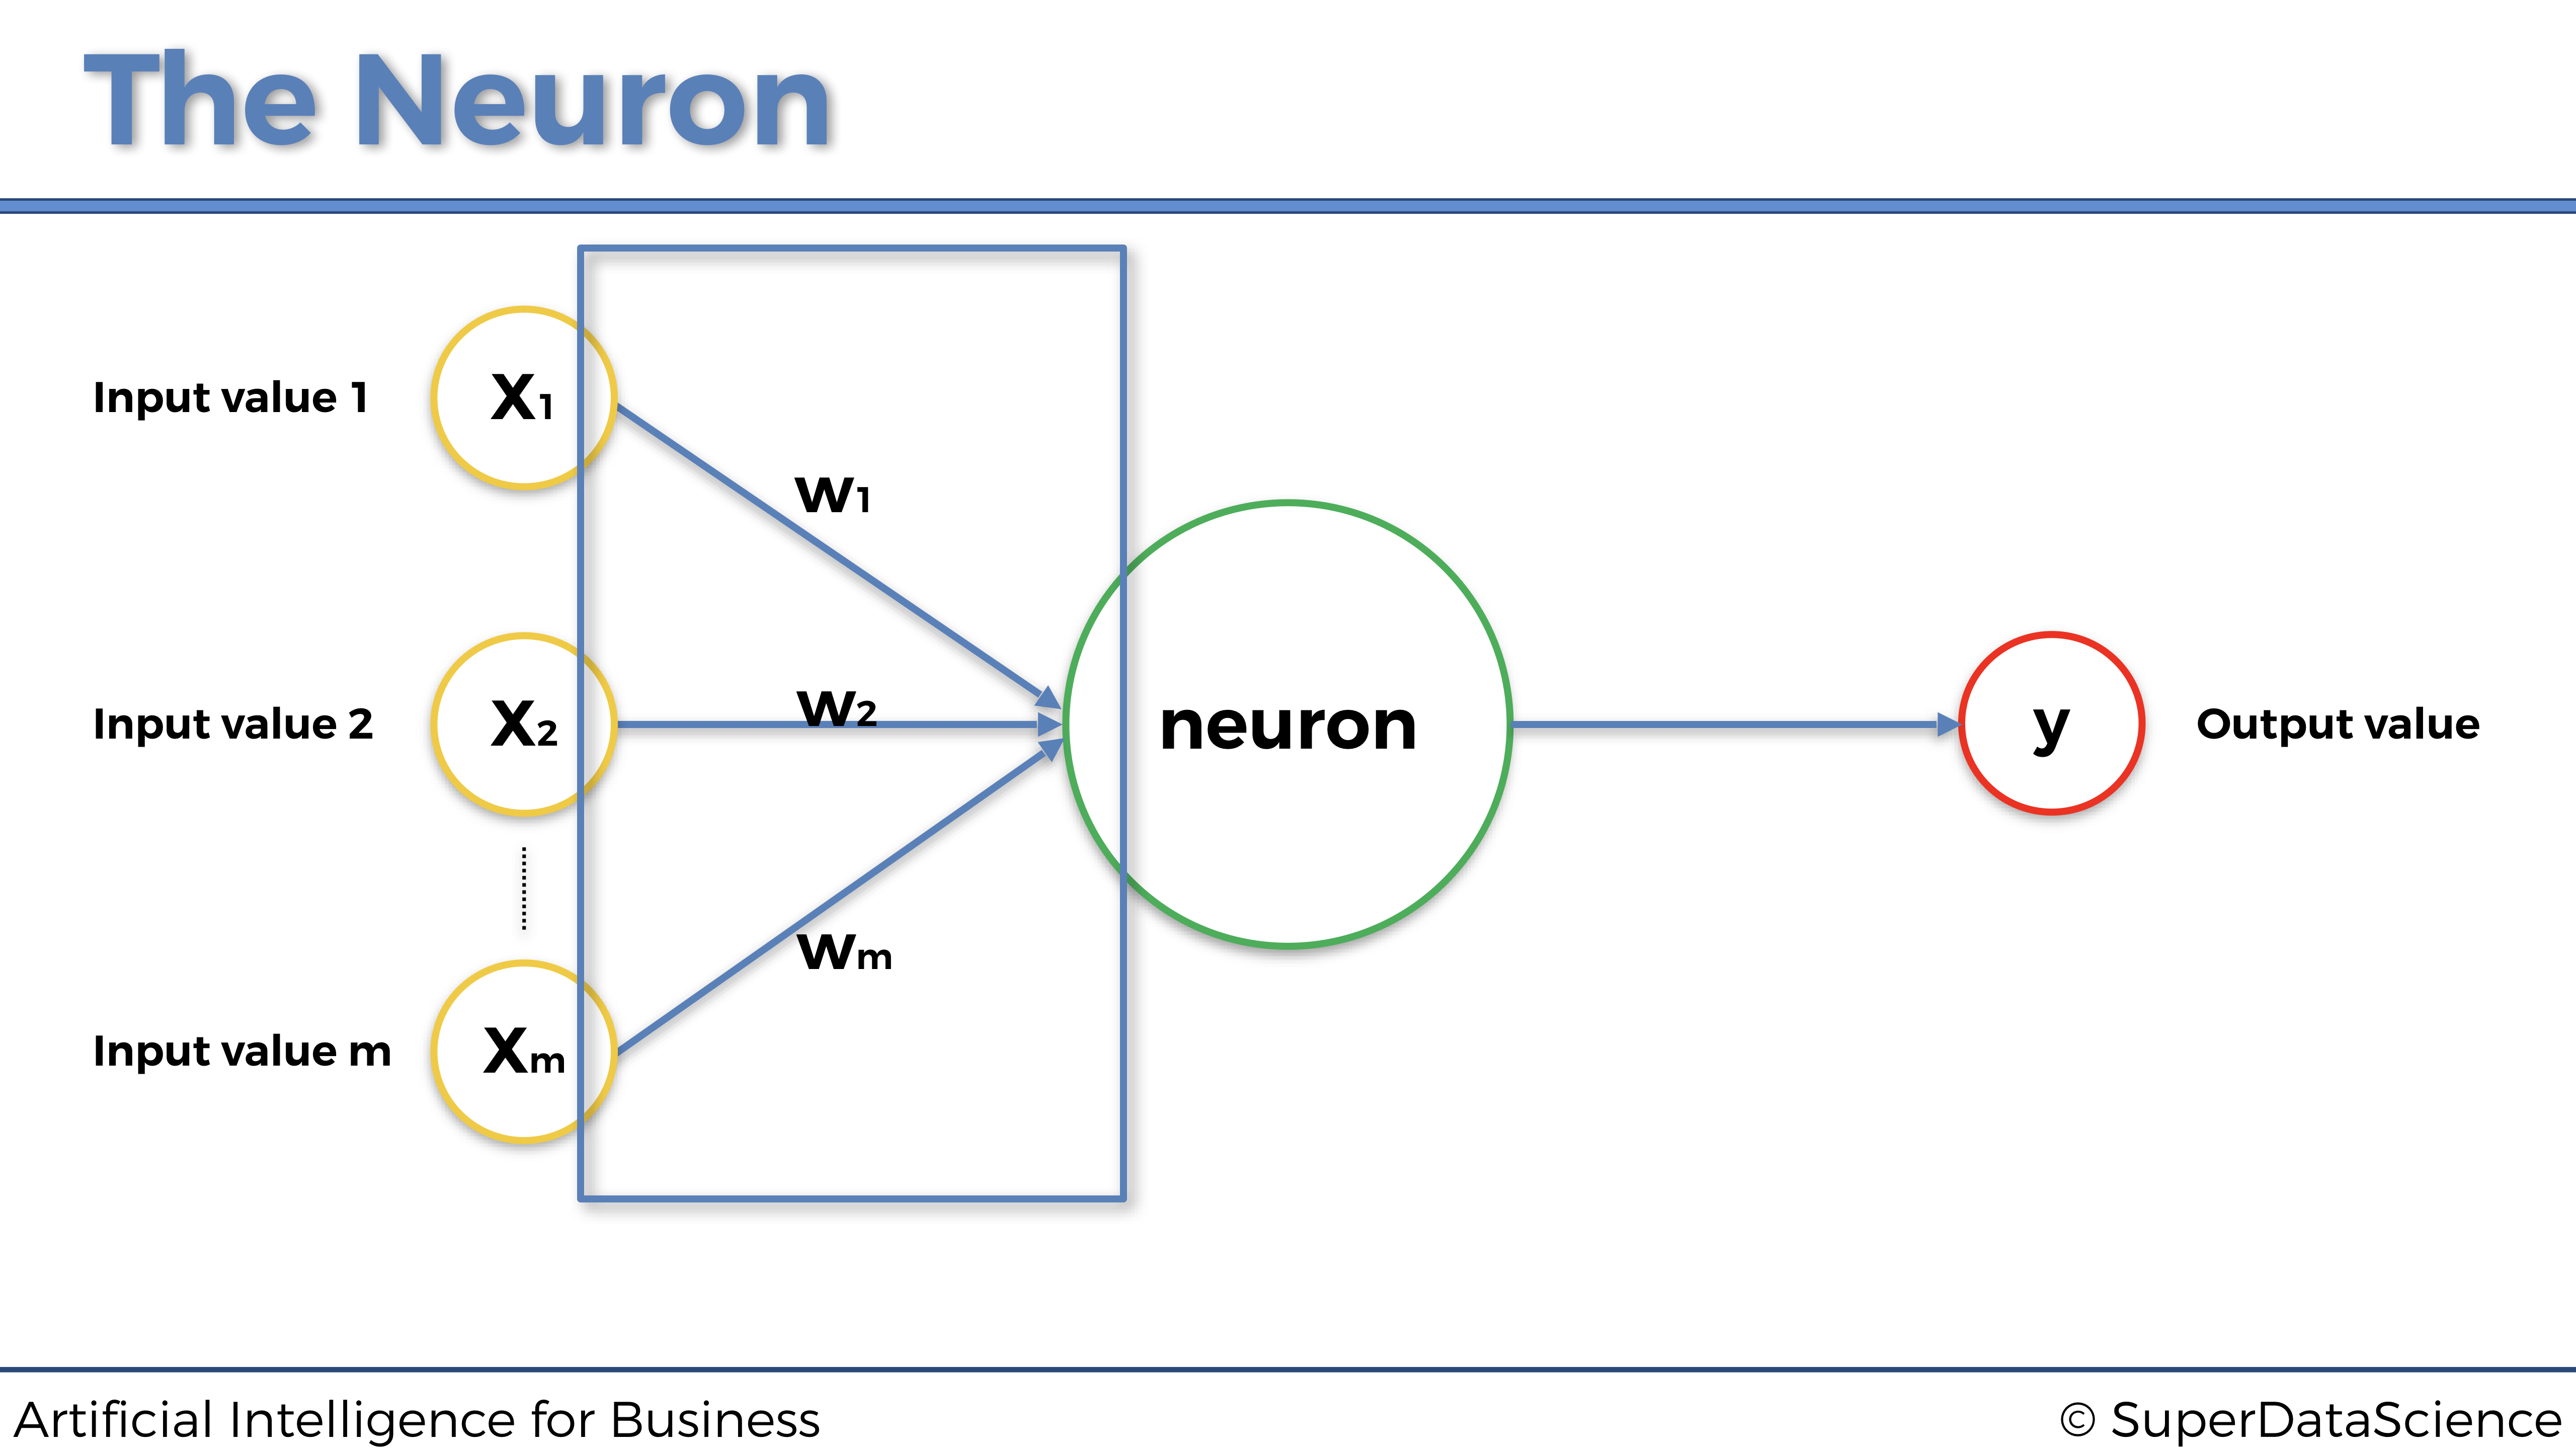
\includegraphics[scale=0.15]{ANN_8.png}
        \end{center}
\end{figure}

\subsection{The Activation Function}

The Activation Function is the function \(\phi\) operating inside the neuron, that will take as inputs the linear sum of the input values multiplied by their associated weights, and that will return the output value:

\begin{figure}[!htbp]
        \begin{center}
            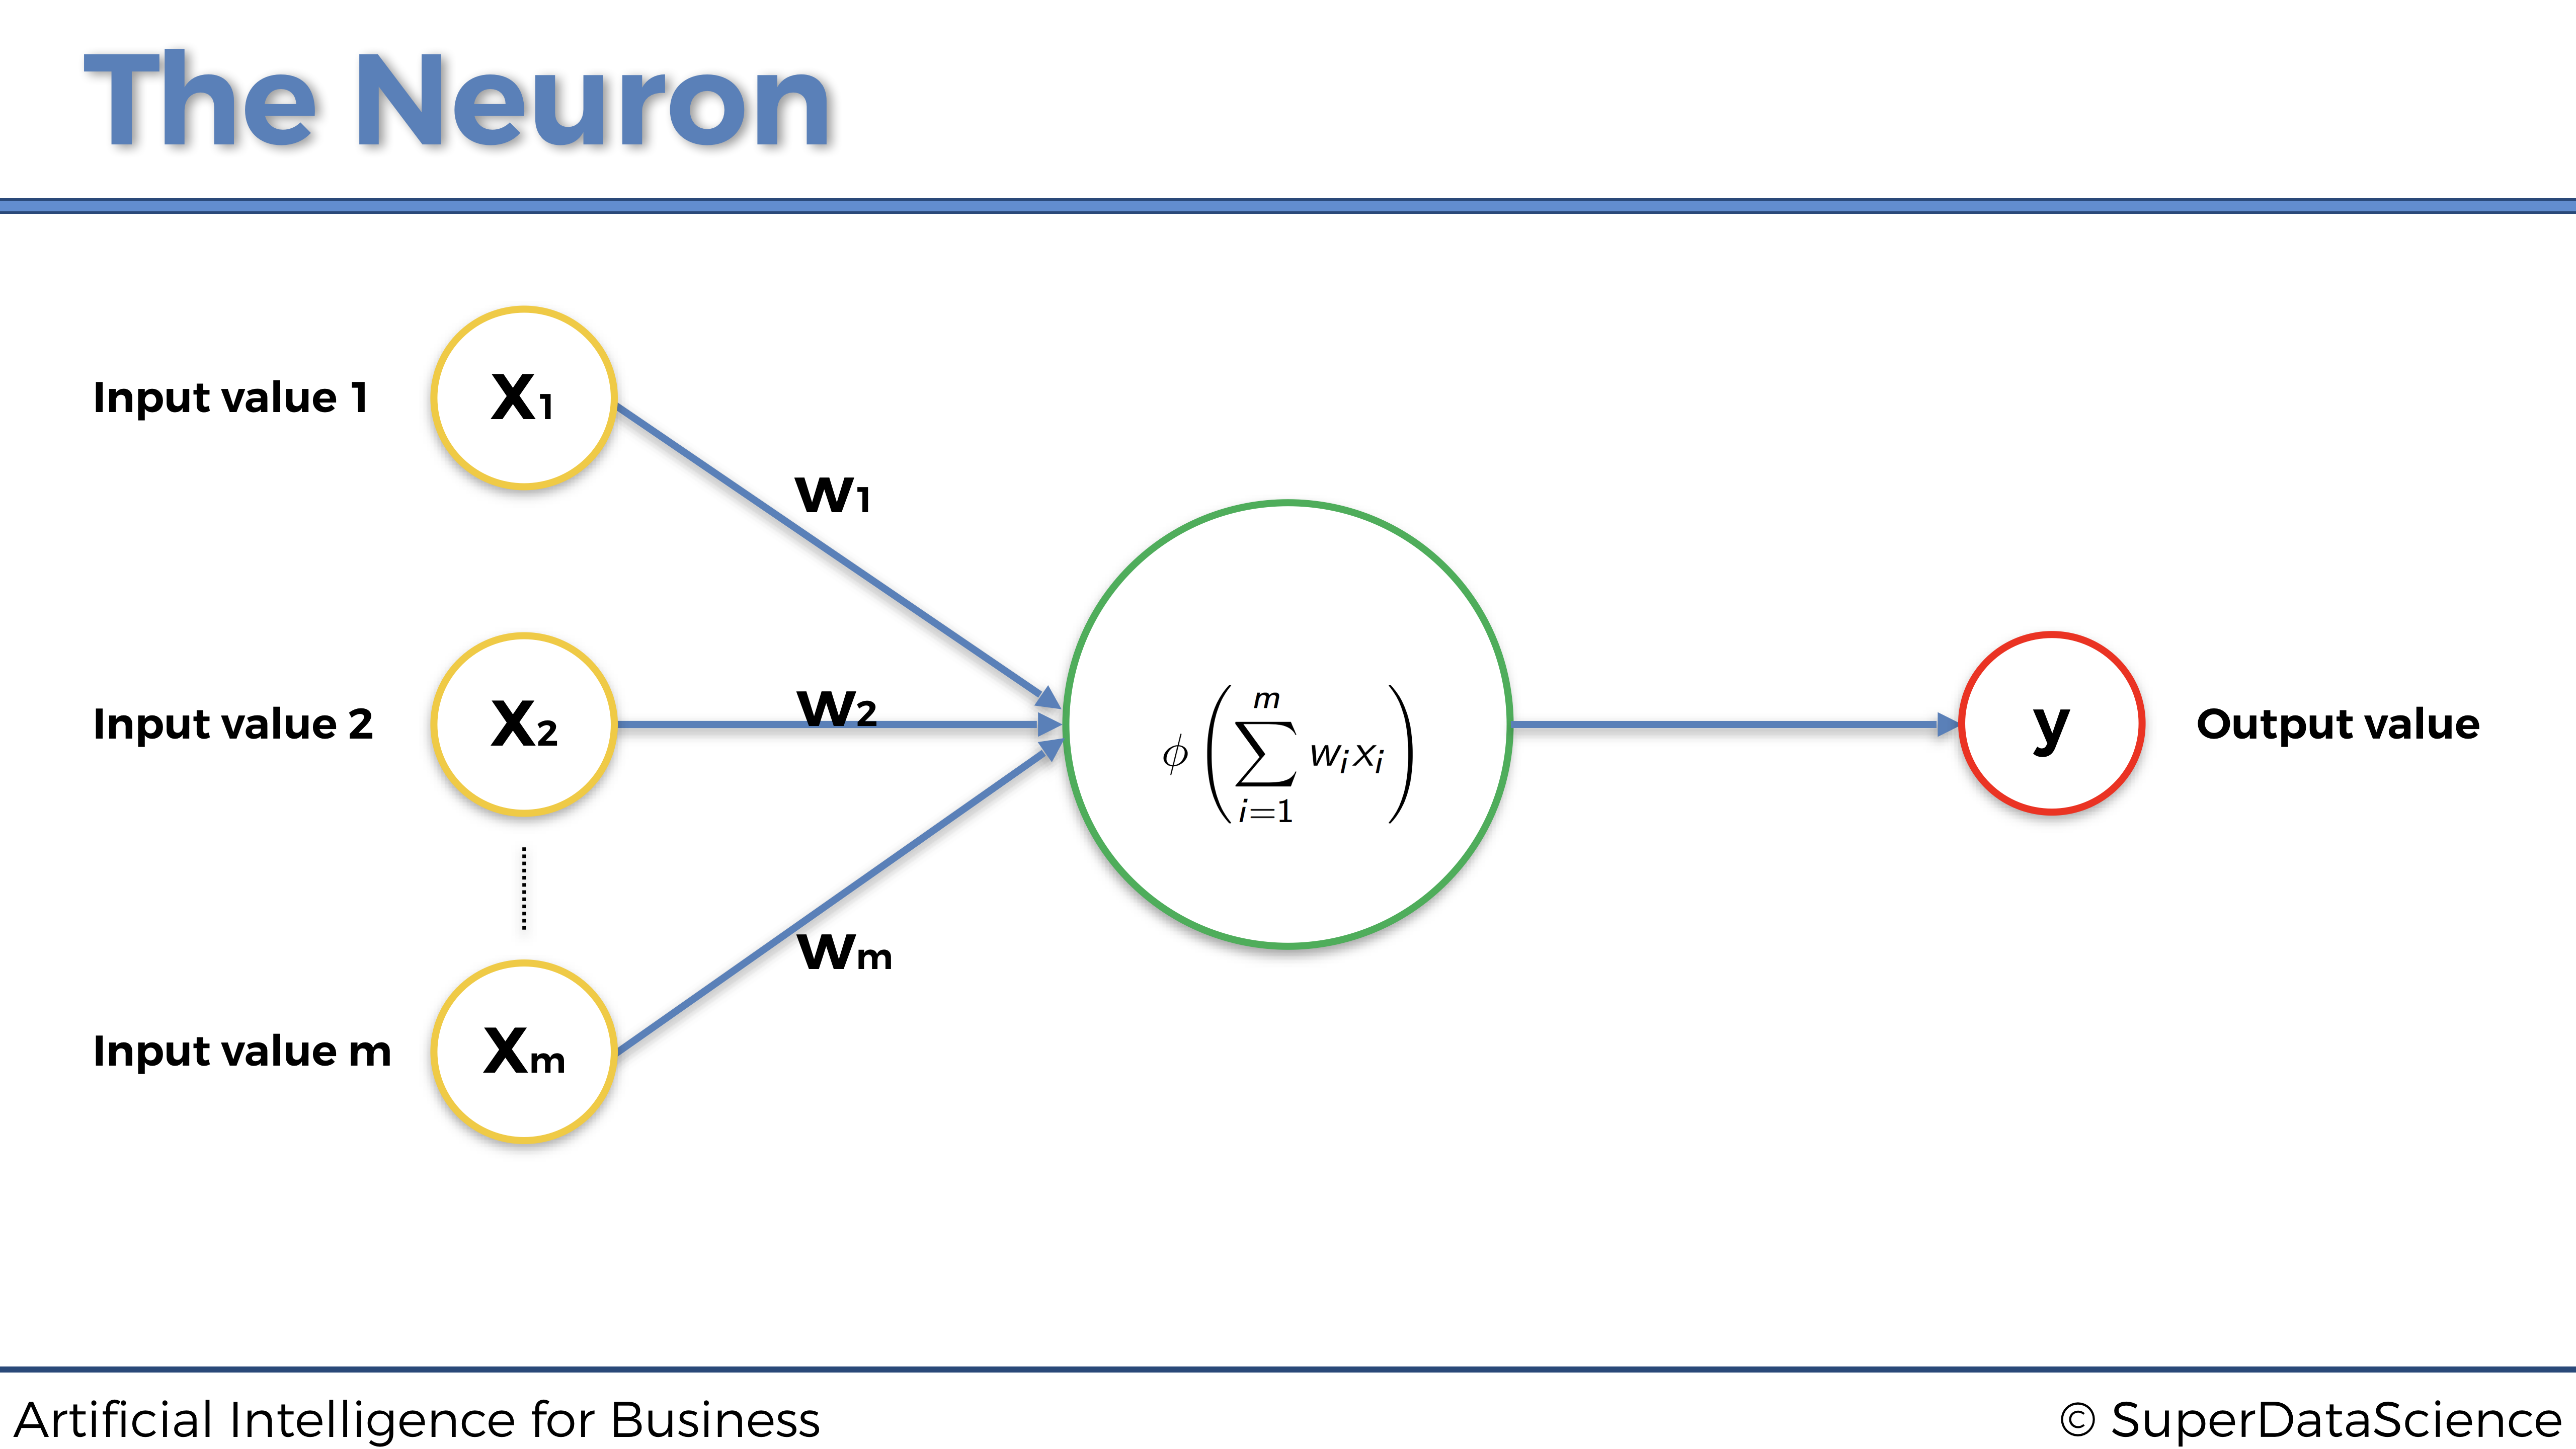
\includegraphics[scale=0.18]{ANN_9.png}
        \end{center}
\end{figure}

such that:

\begin{equation*}
    y = \phi\left( \sum_{i=1}^m w_i x_i \right)
\end{equation*}

Now what exactly is going to be the function \(\phi\)?

There can be many of them, but let's give the four most used ones, including of course the one we used in Part 2 - Minimizing Costs:

\begin{enumerate}
    \item The Threshold Activation Function
    \item The Sigmoid Activation Function
    \item The Rectifier Activation Function
    \item The Hyperbolic Tangent Activation Function
\end{enumerate}

Let's have a look at them one by one.

\newpage

\subsubsection{The Threshold Activation Function}

The Threshold Activation Function is simply defined by the following:

\begin{equation*}
    \phi(x) =
    \begin{cases}
        1 \textrm{ if } x \ge 0 \\
        0 \textrm{ if } x < 0
    \end{cases}
\end{equation*}

so that we get the following curve:

\begin{figure}[!htbp]
        \begin{center}
            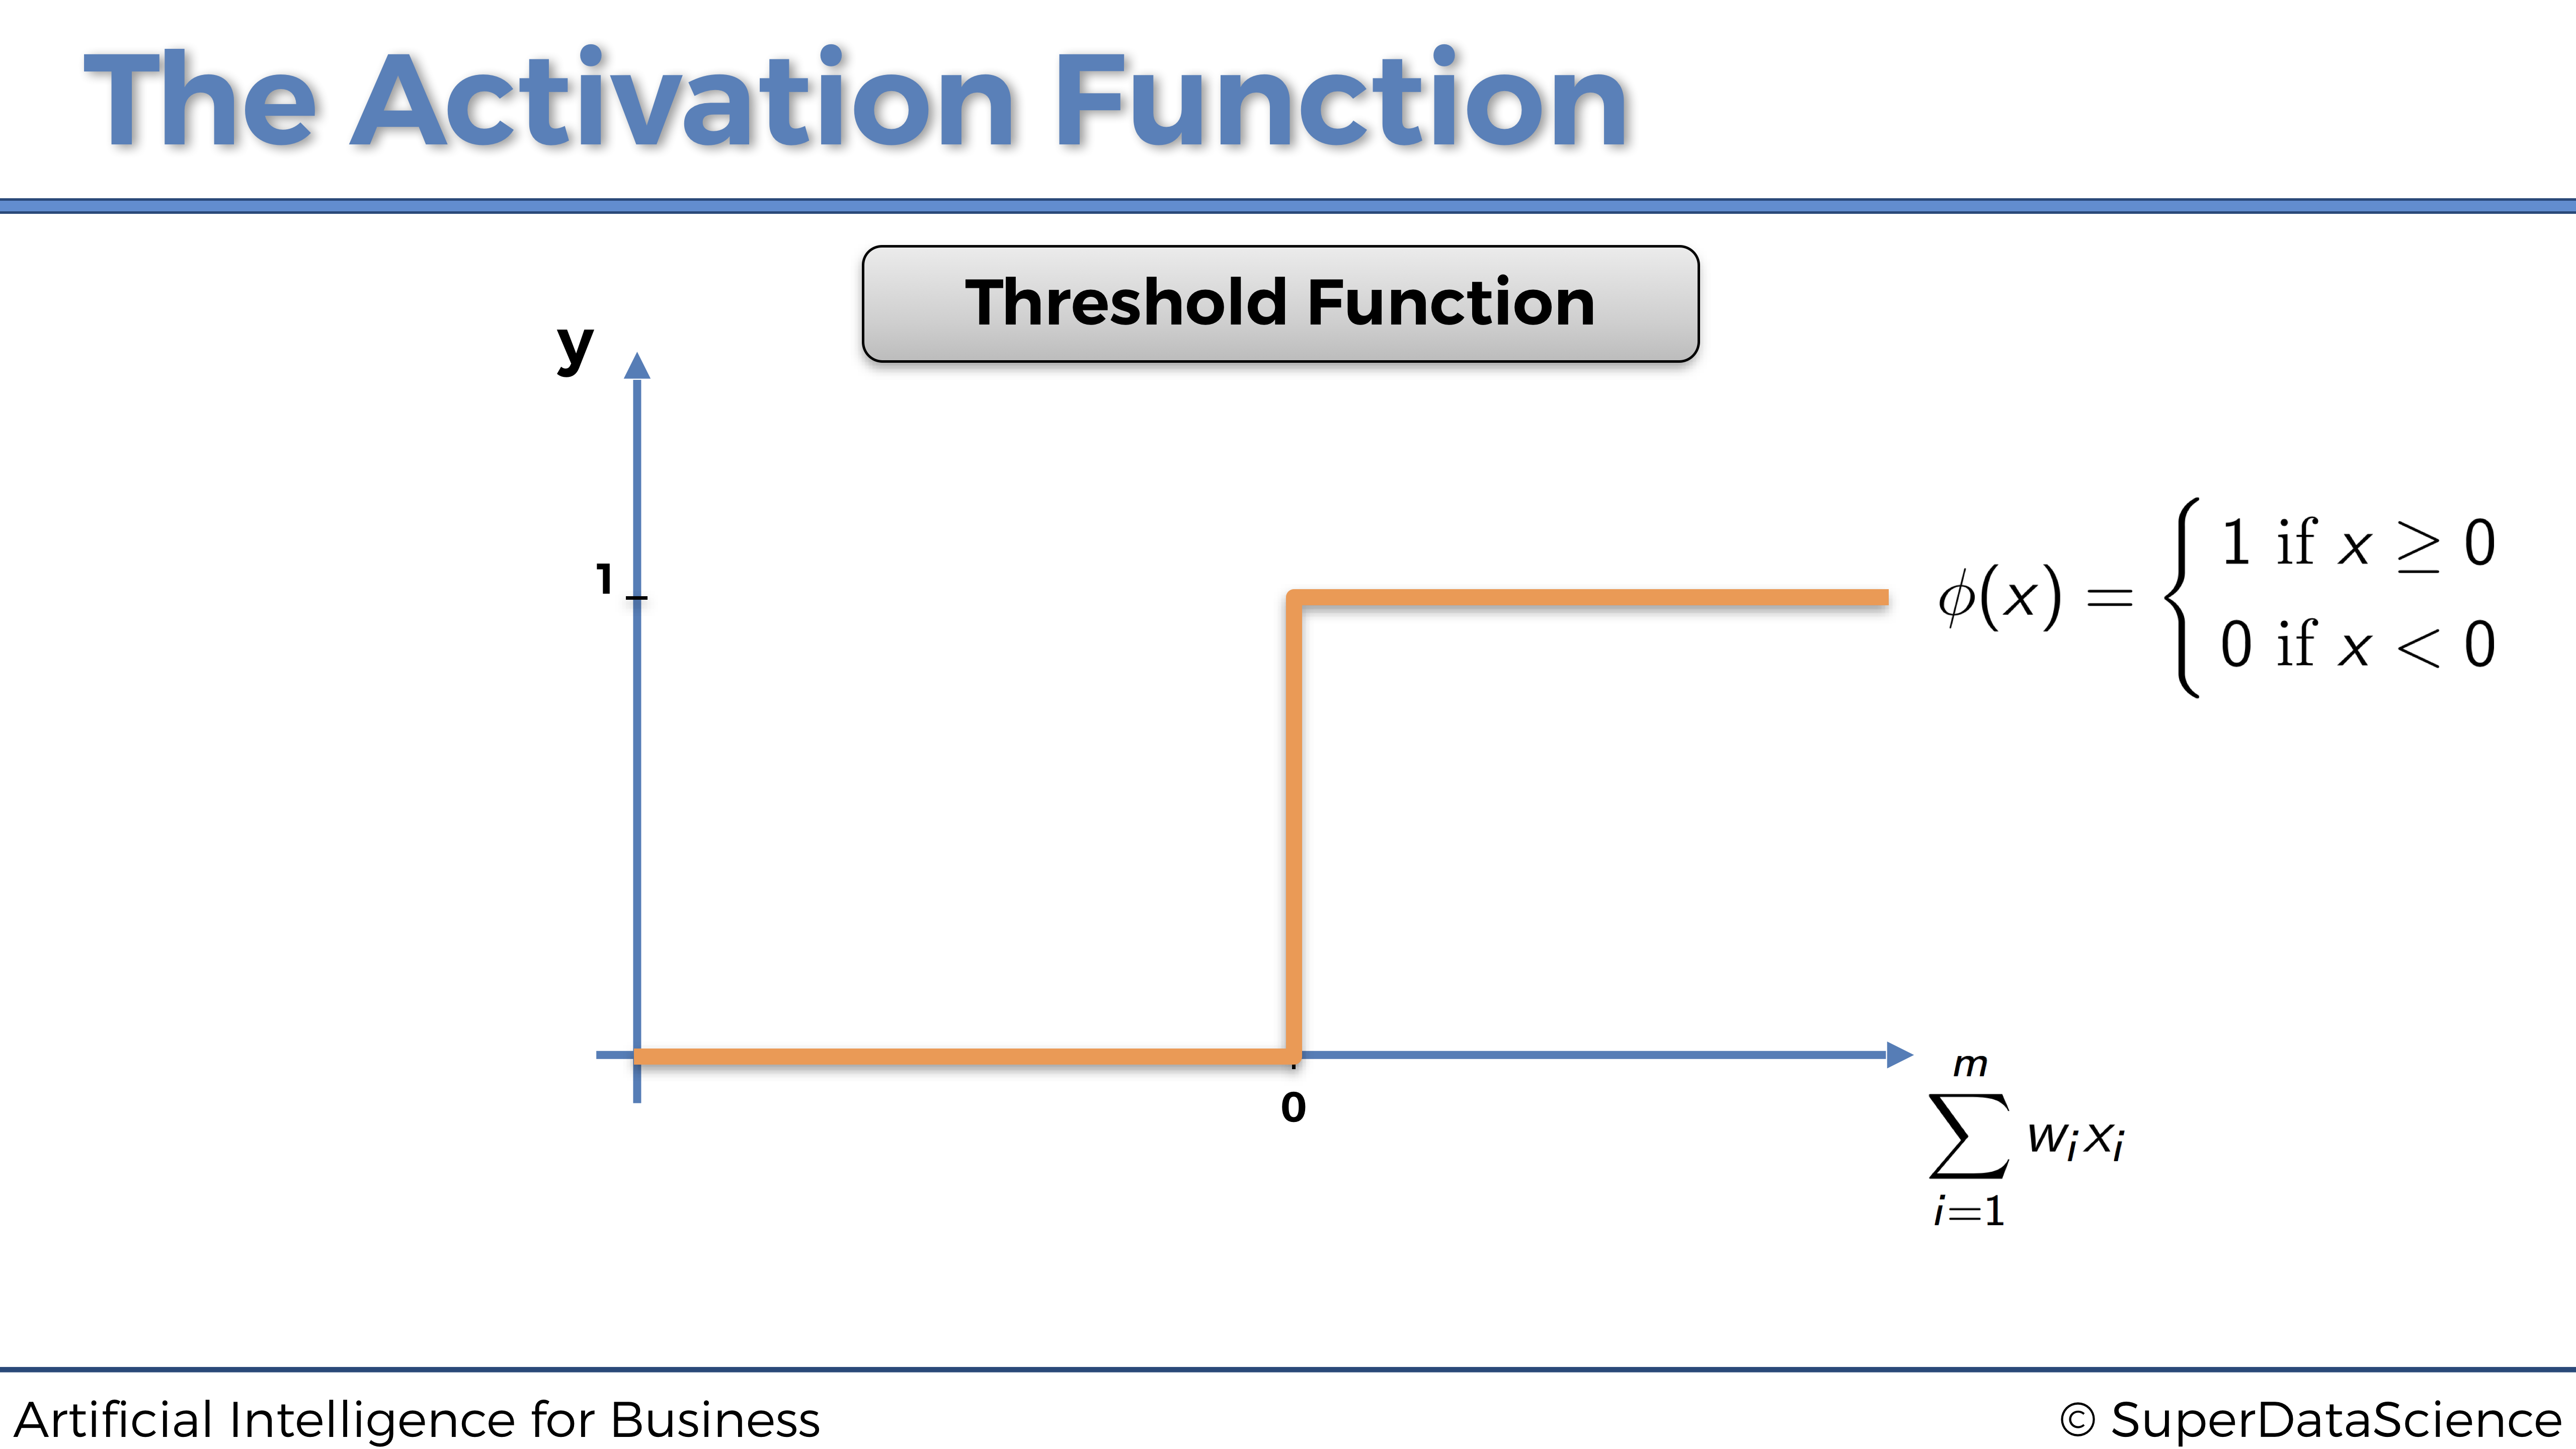
\includegraphics[scale=0.18]{ANN_10.png}
        \end{center}
\end{figure}

This means that the signal passing through the neuron will be discontinuous, and will only be activated if:

\begin{equation*}
    \sum_{i=1}^m w_i x_i \ge 0
\end{equation*}

Now let's have a look at the next activation function: the Sigmoid Activation function.

The Sigmoid Activation Function is the most effective and widely used one in Artificial Neural Networks, but mostly inside the last hidden layer (if we are dealing with a Deep Neural Network composed of several hidden layers) passing the signal towards the output layer.

\newpage

\subsubsection{The Sigmoid Activation Function}

The Sigmoid Activation Function is defined by the following:

\begin{equation*}
\phi(x) = \frac{1}{1+e^{-x}}
\end{equation*}

so that we get the following curve:

\begin{figure}[!htbp]
        \begin{center}
            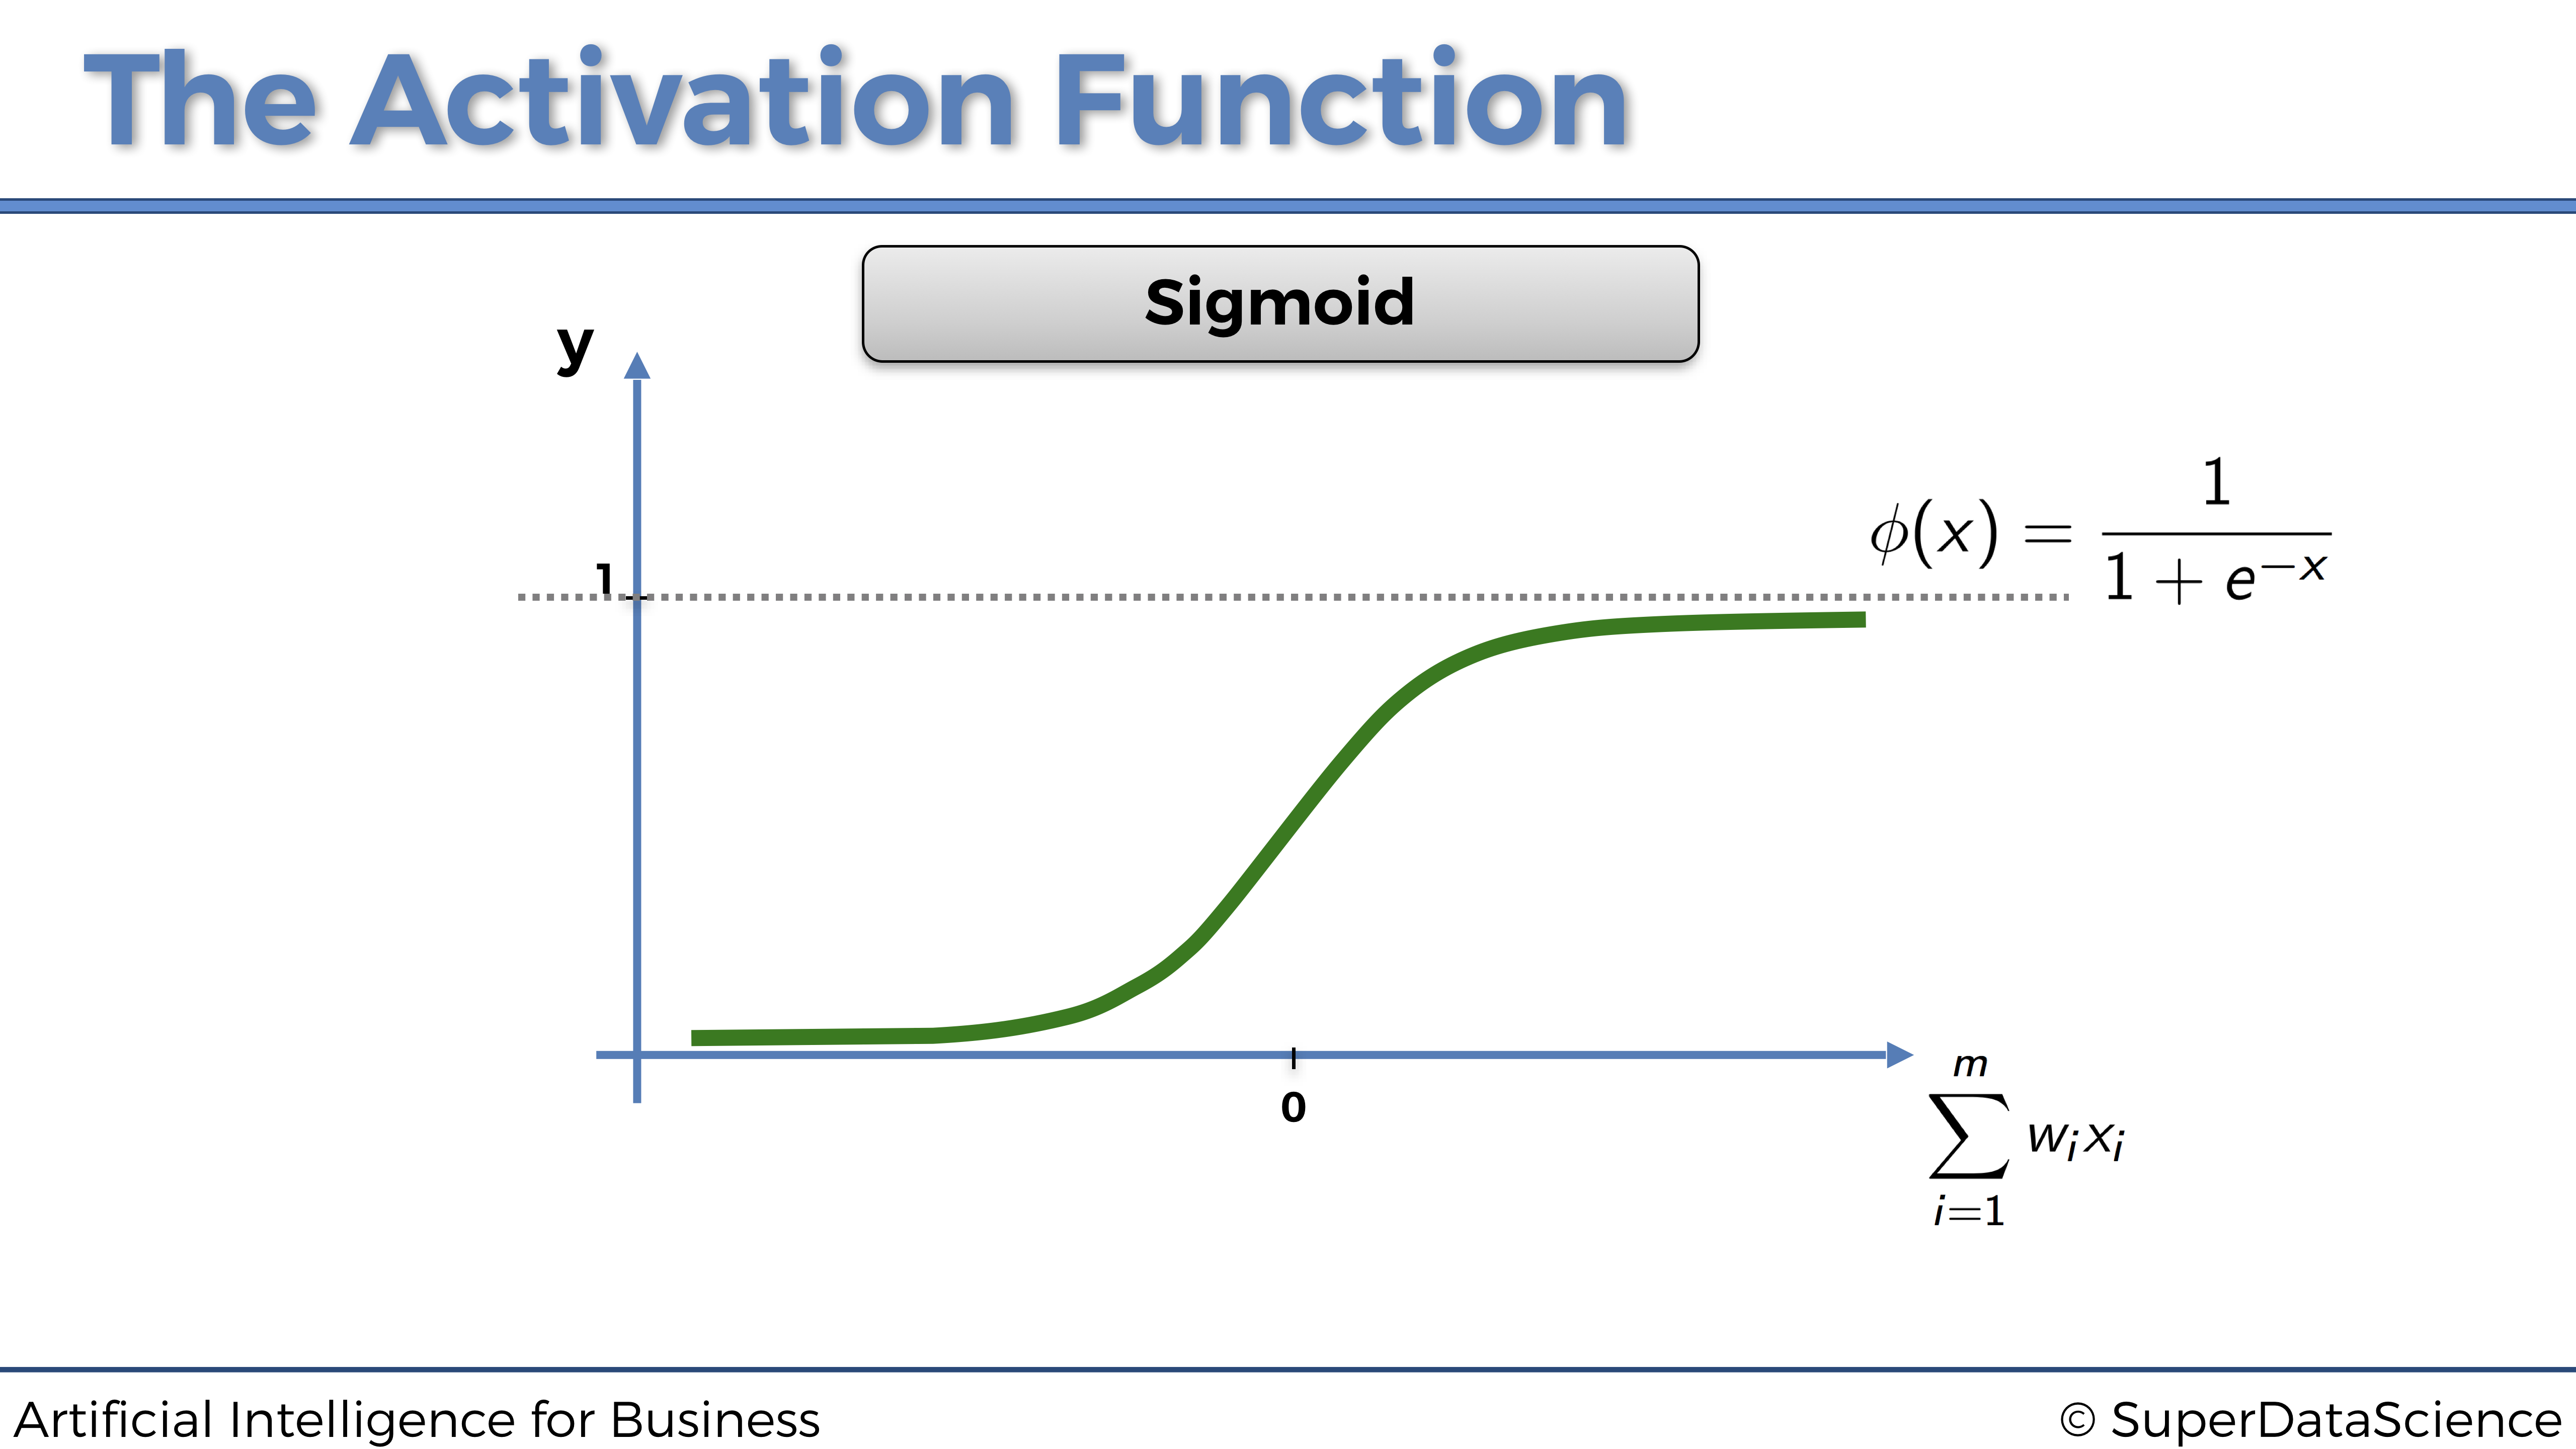
\includegraphics[scale=0.18]{ANN_11.png}
        \end{center}
\end{figure}

This means that the signal passing through the neuron will be continuous and will always be activated. And the higher is \(\sum_{i=1}^m w_i x_i\), the stronger will be that signal.

Now let's have a look at another widely used activation function: the Rectifier Activation function.

You will find it in most of the \underline{DEEP} Neural Networks, but mostly inside the hidden layers, as opposed to the sigmoid function which is rather used for the output layer.

\newpage

\subsubsection{The Rectifier Activation Function}

The Threshold Activation Function is simply defined by the following:

\begin{equation*}
    \phi(x) = \max(x,0)
\end{equation*}

so that we get the following curve:

\begin{figure}[!htbp]
        \begin{center}
            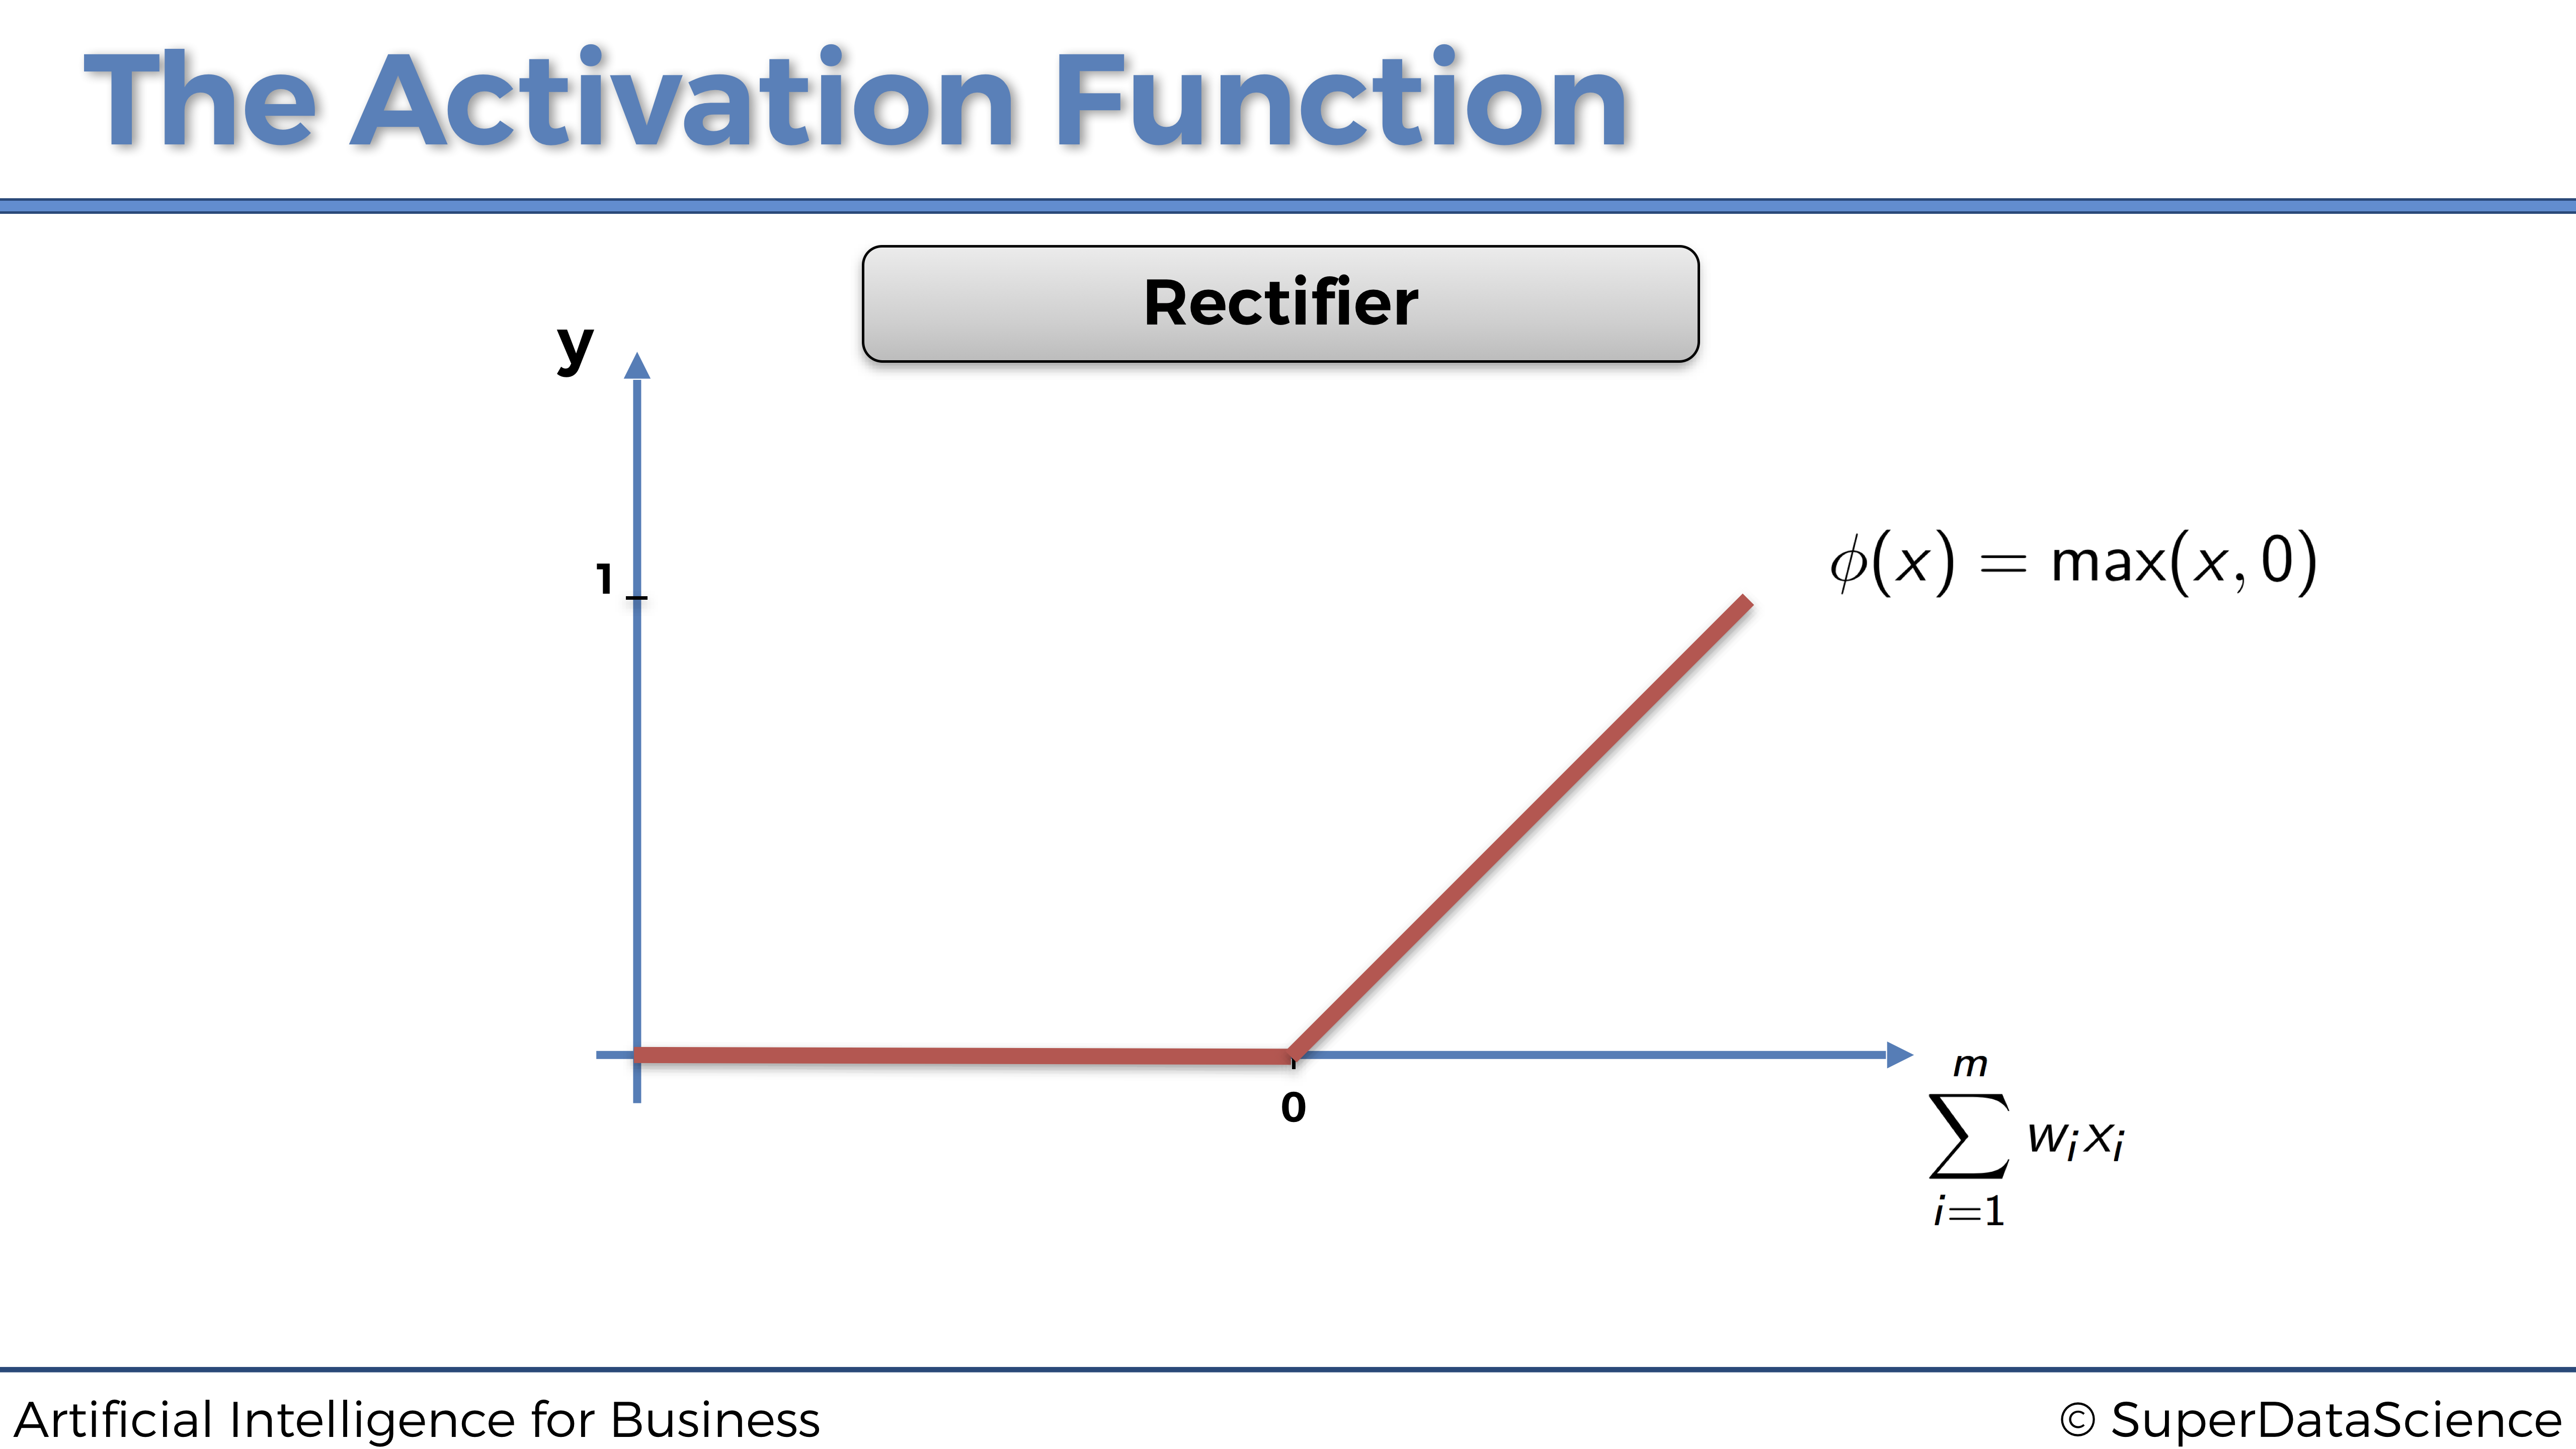
\includegraphics[scale=0.18]{ANN_12.png}
        \end{center}
\end{figure}

This means that the signal passing through the neuron will be continuous, and will only be activated if:

\begin{equation*}
    \sum_{i=1}^m w_i x_i \ge 0
\end{equation*}

And the higher is \(\sum_{i=1}^m w_i x_i\) above 0, the stronger will be that signal.

Now let's have a look at the next activation function: the Hyperbolic Tangent Activation function.

The Hyperbolic Tangent activation function is less widely used, though it can sometimes be a more relevant choice in some Artificial Neural Networks, especially when the inputs are standardized.

\newpage

\subsubsection{The Hyperbolic Tangent Activation Function}

The Hyperbolic Tangent Activation Function is defined by the following:

\begin{equation*}
    \phi(x) = \frac{1-e^{-2x}}{1+e^{-2x}}
\end{equation*}

so that we get the following curve:

\begin{figure}[!htbp]
        \begin{center}
            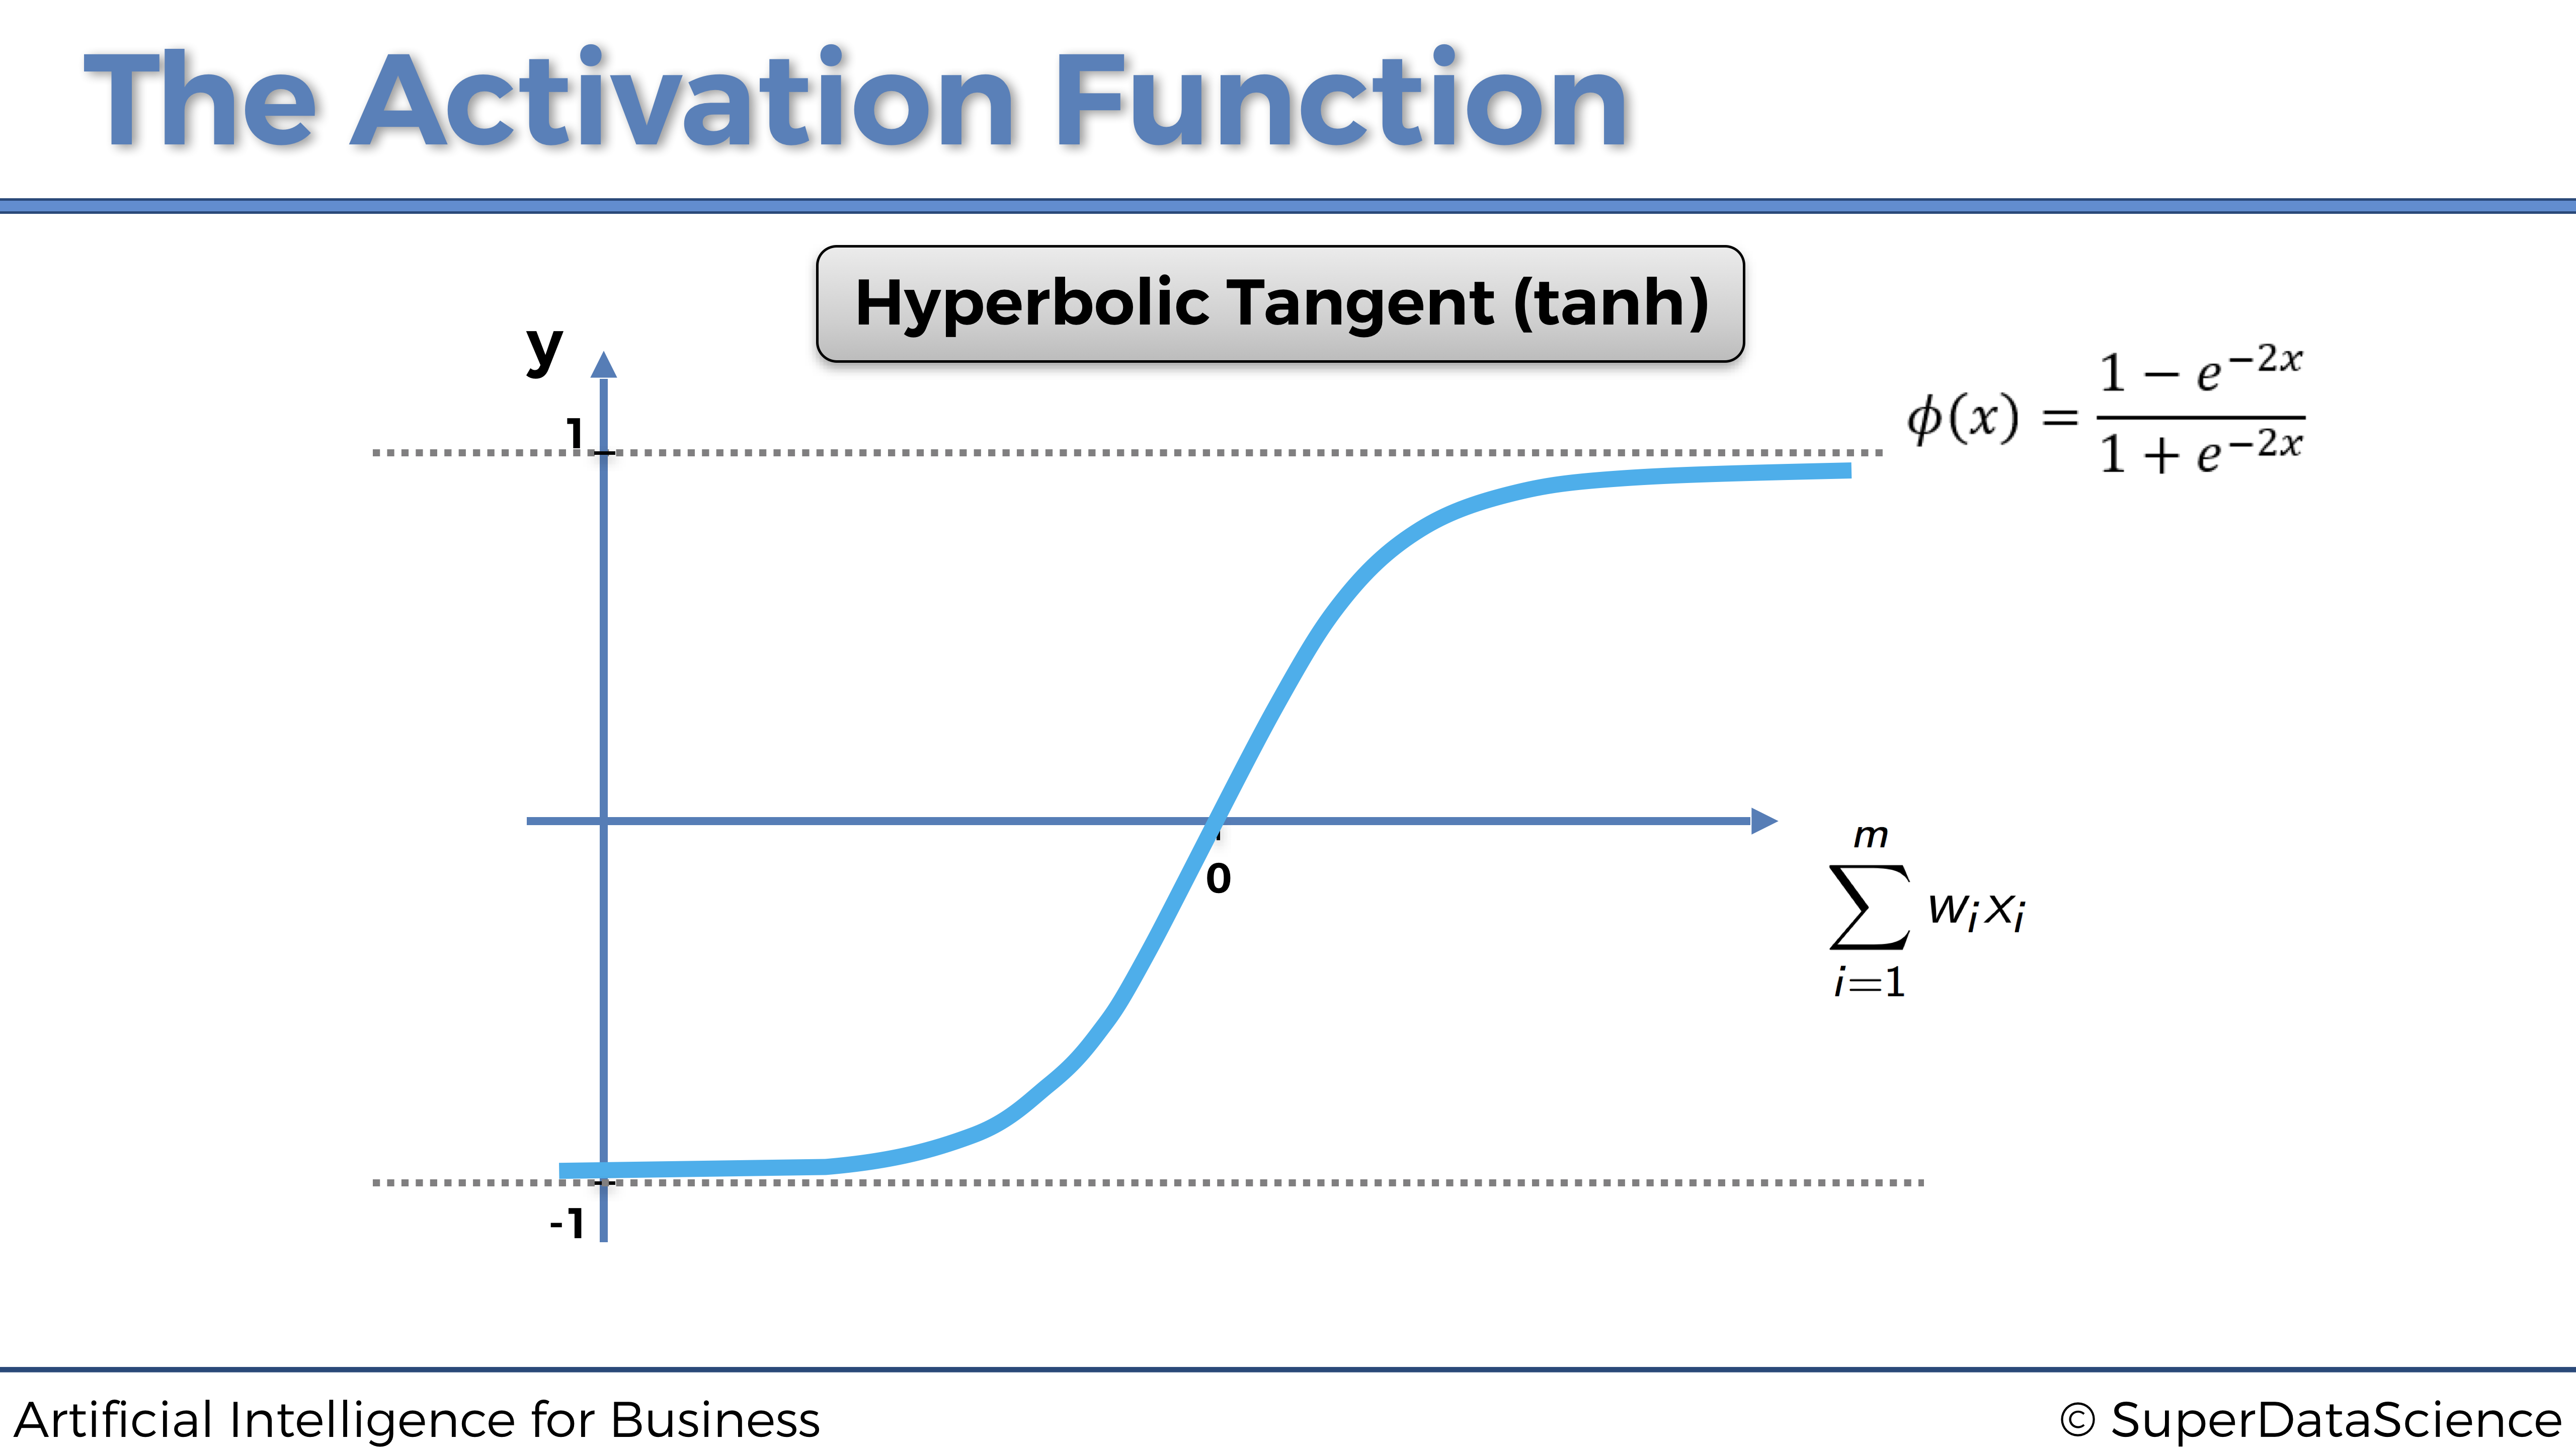
\includegraphics[scale=0.18]{ANN_13.png}
        \end{center}
\end{figure}

This means that the signal passing through the neuron will be continuous and will always be activated. The higher \(\sum_{i=1}^m w_i x_i\) is above 0, the stronger will be that signal. The lower \(\sum_{i=1}^m w_i x_i\) is below 0, the weaker will be that signal.

\newpage

So that raises the question: which activation function should we choose, or, more frequently asked, how do we know which one to choose?

Good news, the answer is simple, and let's give it inside a small blueprint.

That actually depends on what is returned as the dependent variable. If it is a binary outcome 0 or 1, then a good choice would be the threshold activation function. If what you want to be returned is the probability that the dependent variable is 1, then an excellent choice is the sigmoid activation function, since its sigmoid curve is a perfect fit to model probabilities.

Here is this small blueprint highlighted in this slide:

\begin{figure}[!htbp]
        \begin{center}
            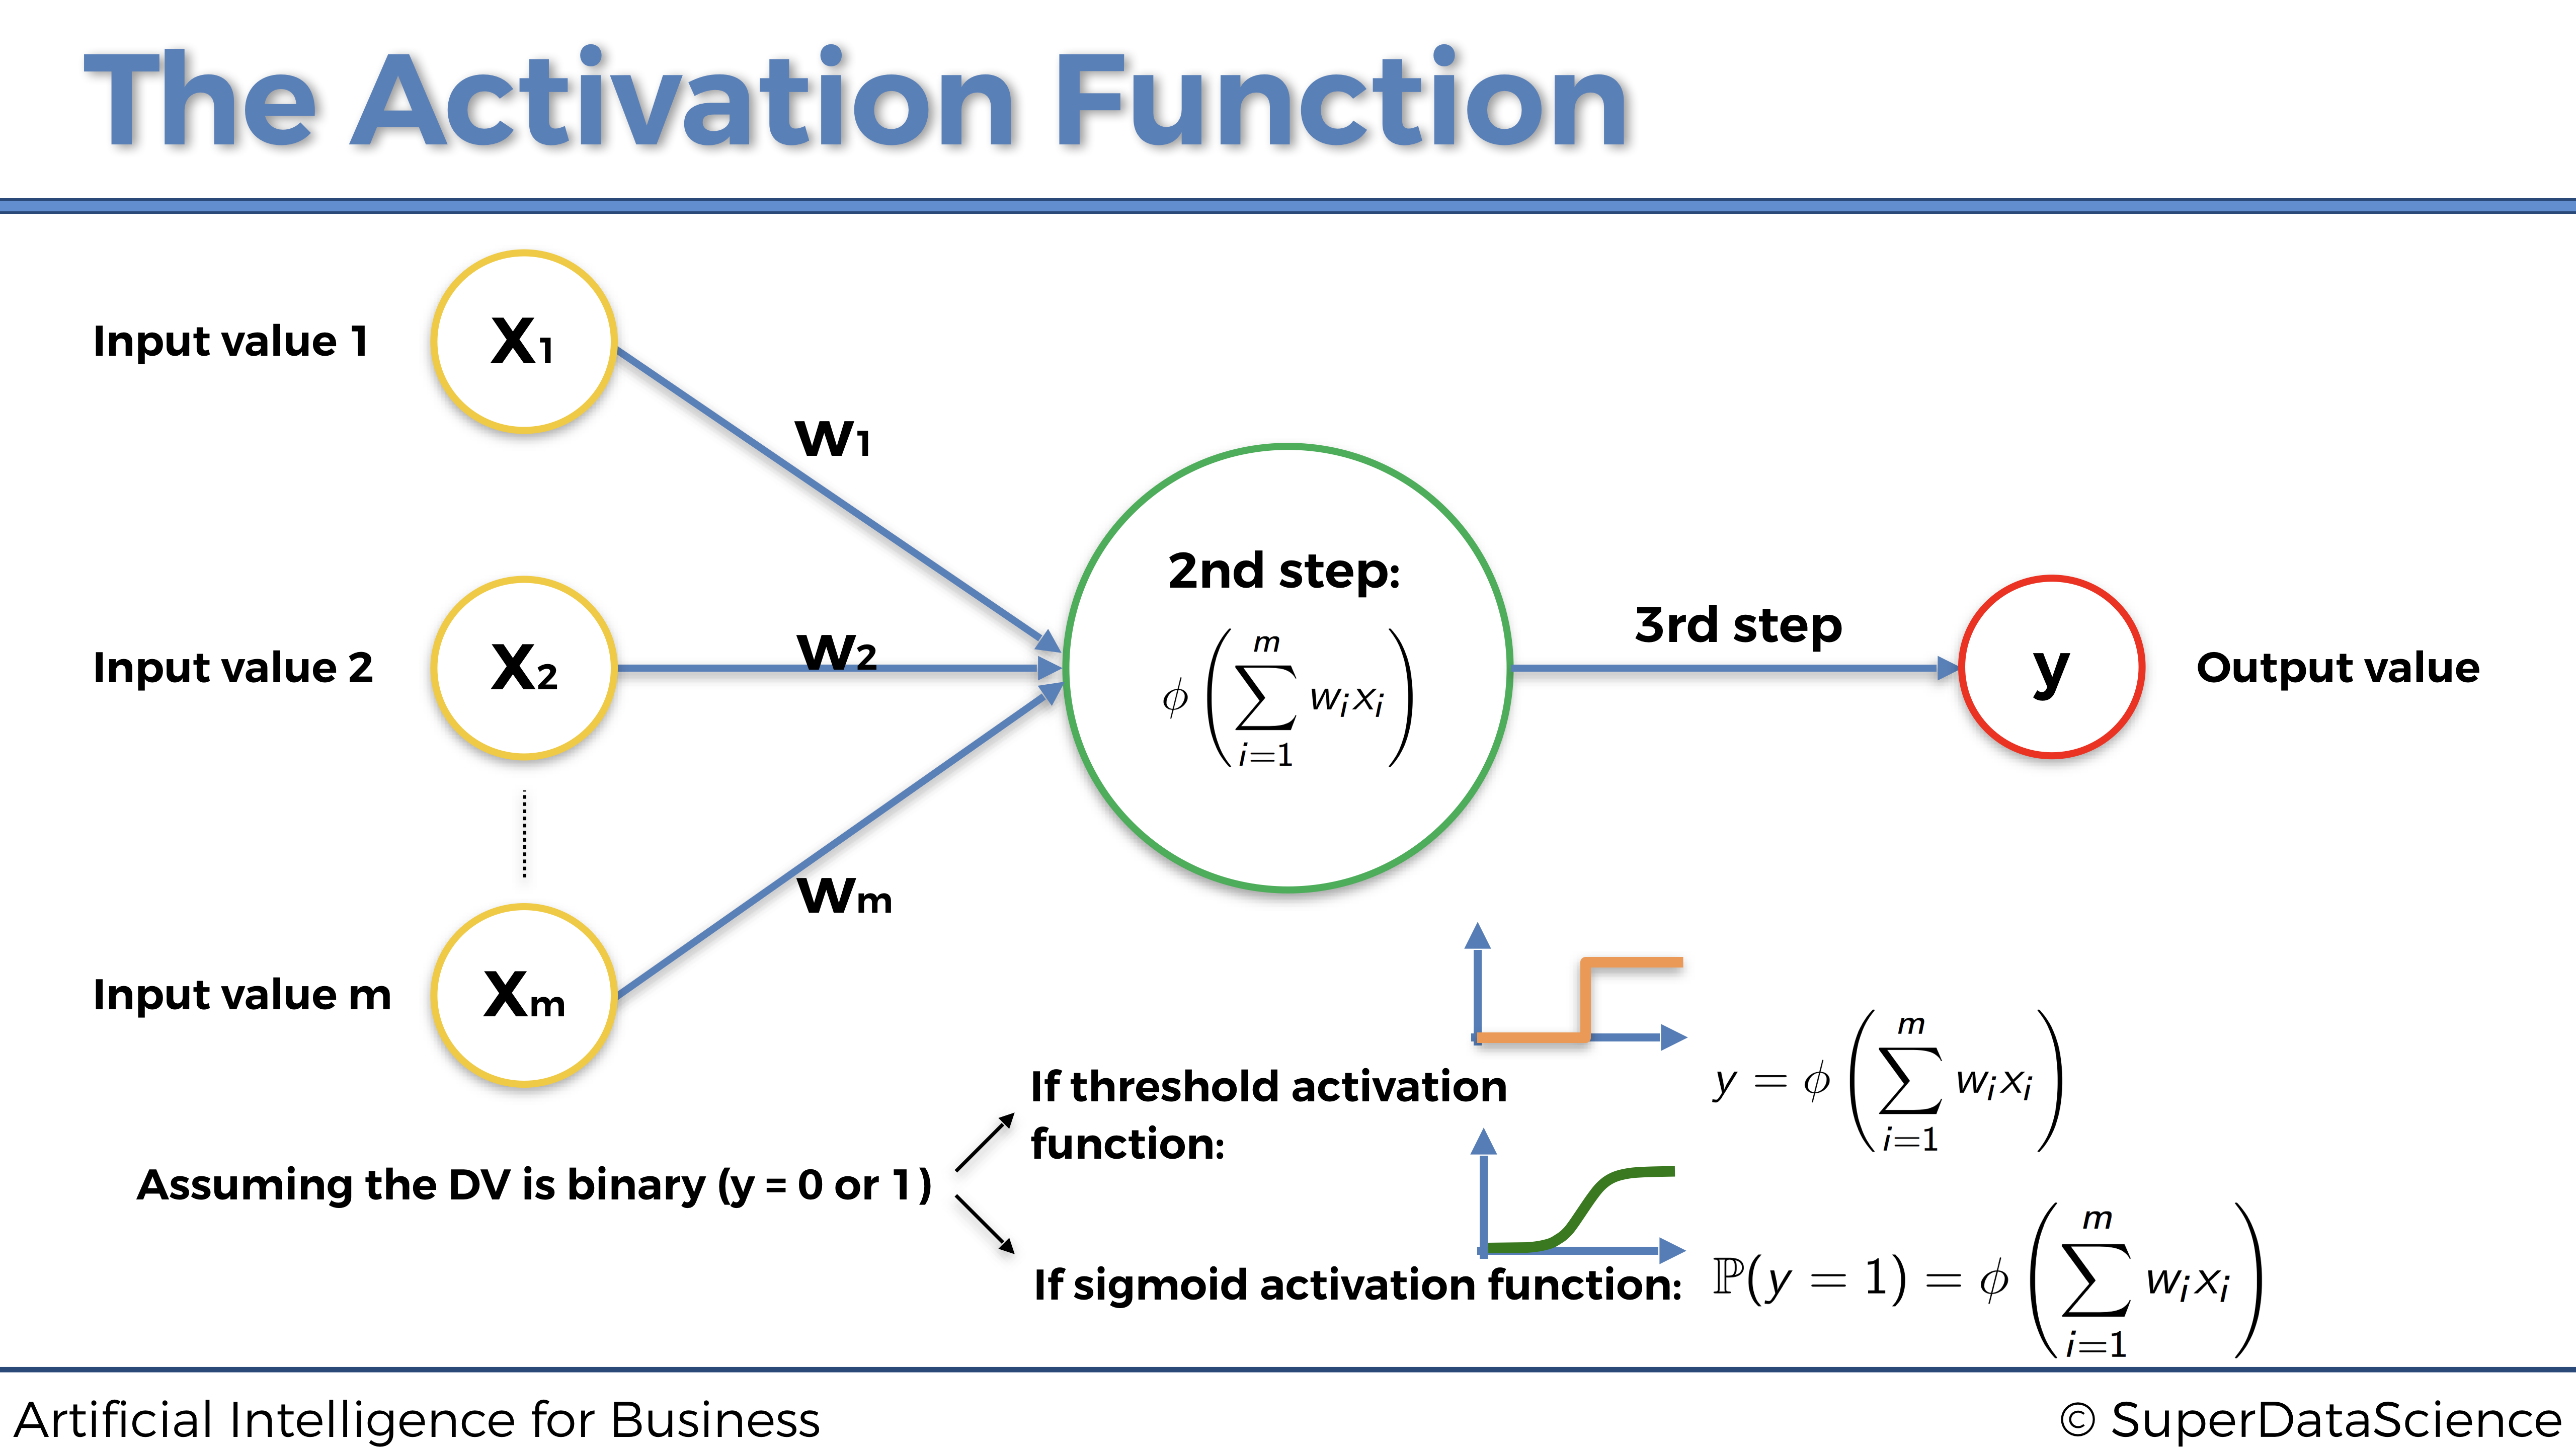
\includegraphics[scale=0.18]{ANN_14.png}
        \end{center}
\end{figure}

But then when should I use the other two activation functions, i.e.~the Rectifier activation function and the Hyperbolic Tangent activation function?

Easy again, the Rectifier and the Hyperbolic Tangent activation functions should be used within the hidden layers of a Deep Neural Network (with more than one hidden layer), except the last hidden layer leading to the output layer for which it is recommended to use a Sigmoid Activation function.

\newpage

Let's recap this again inside the following slide:

\begin{figure}[!htbp]
        \begin{center}
            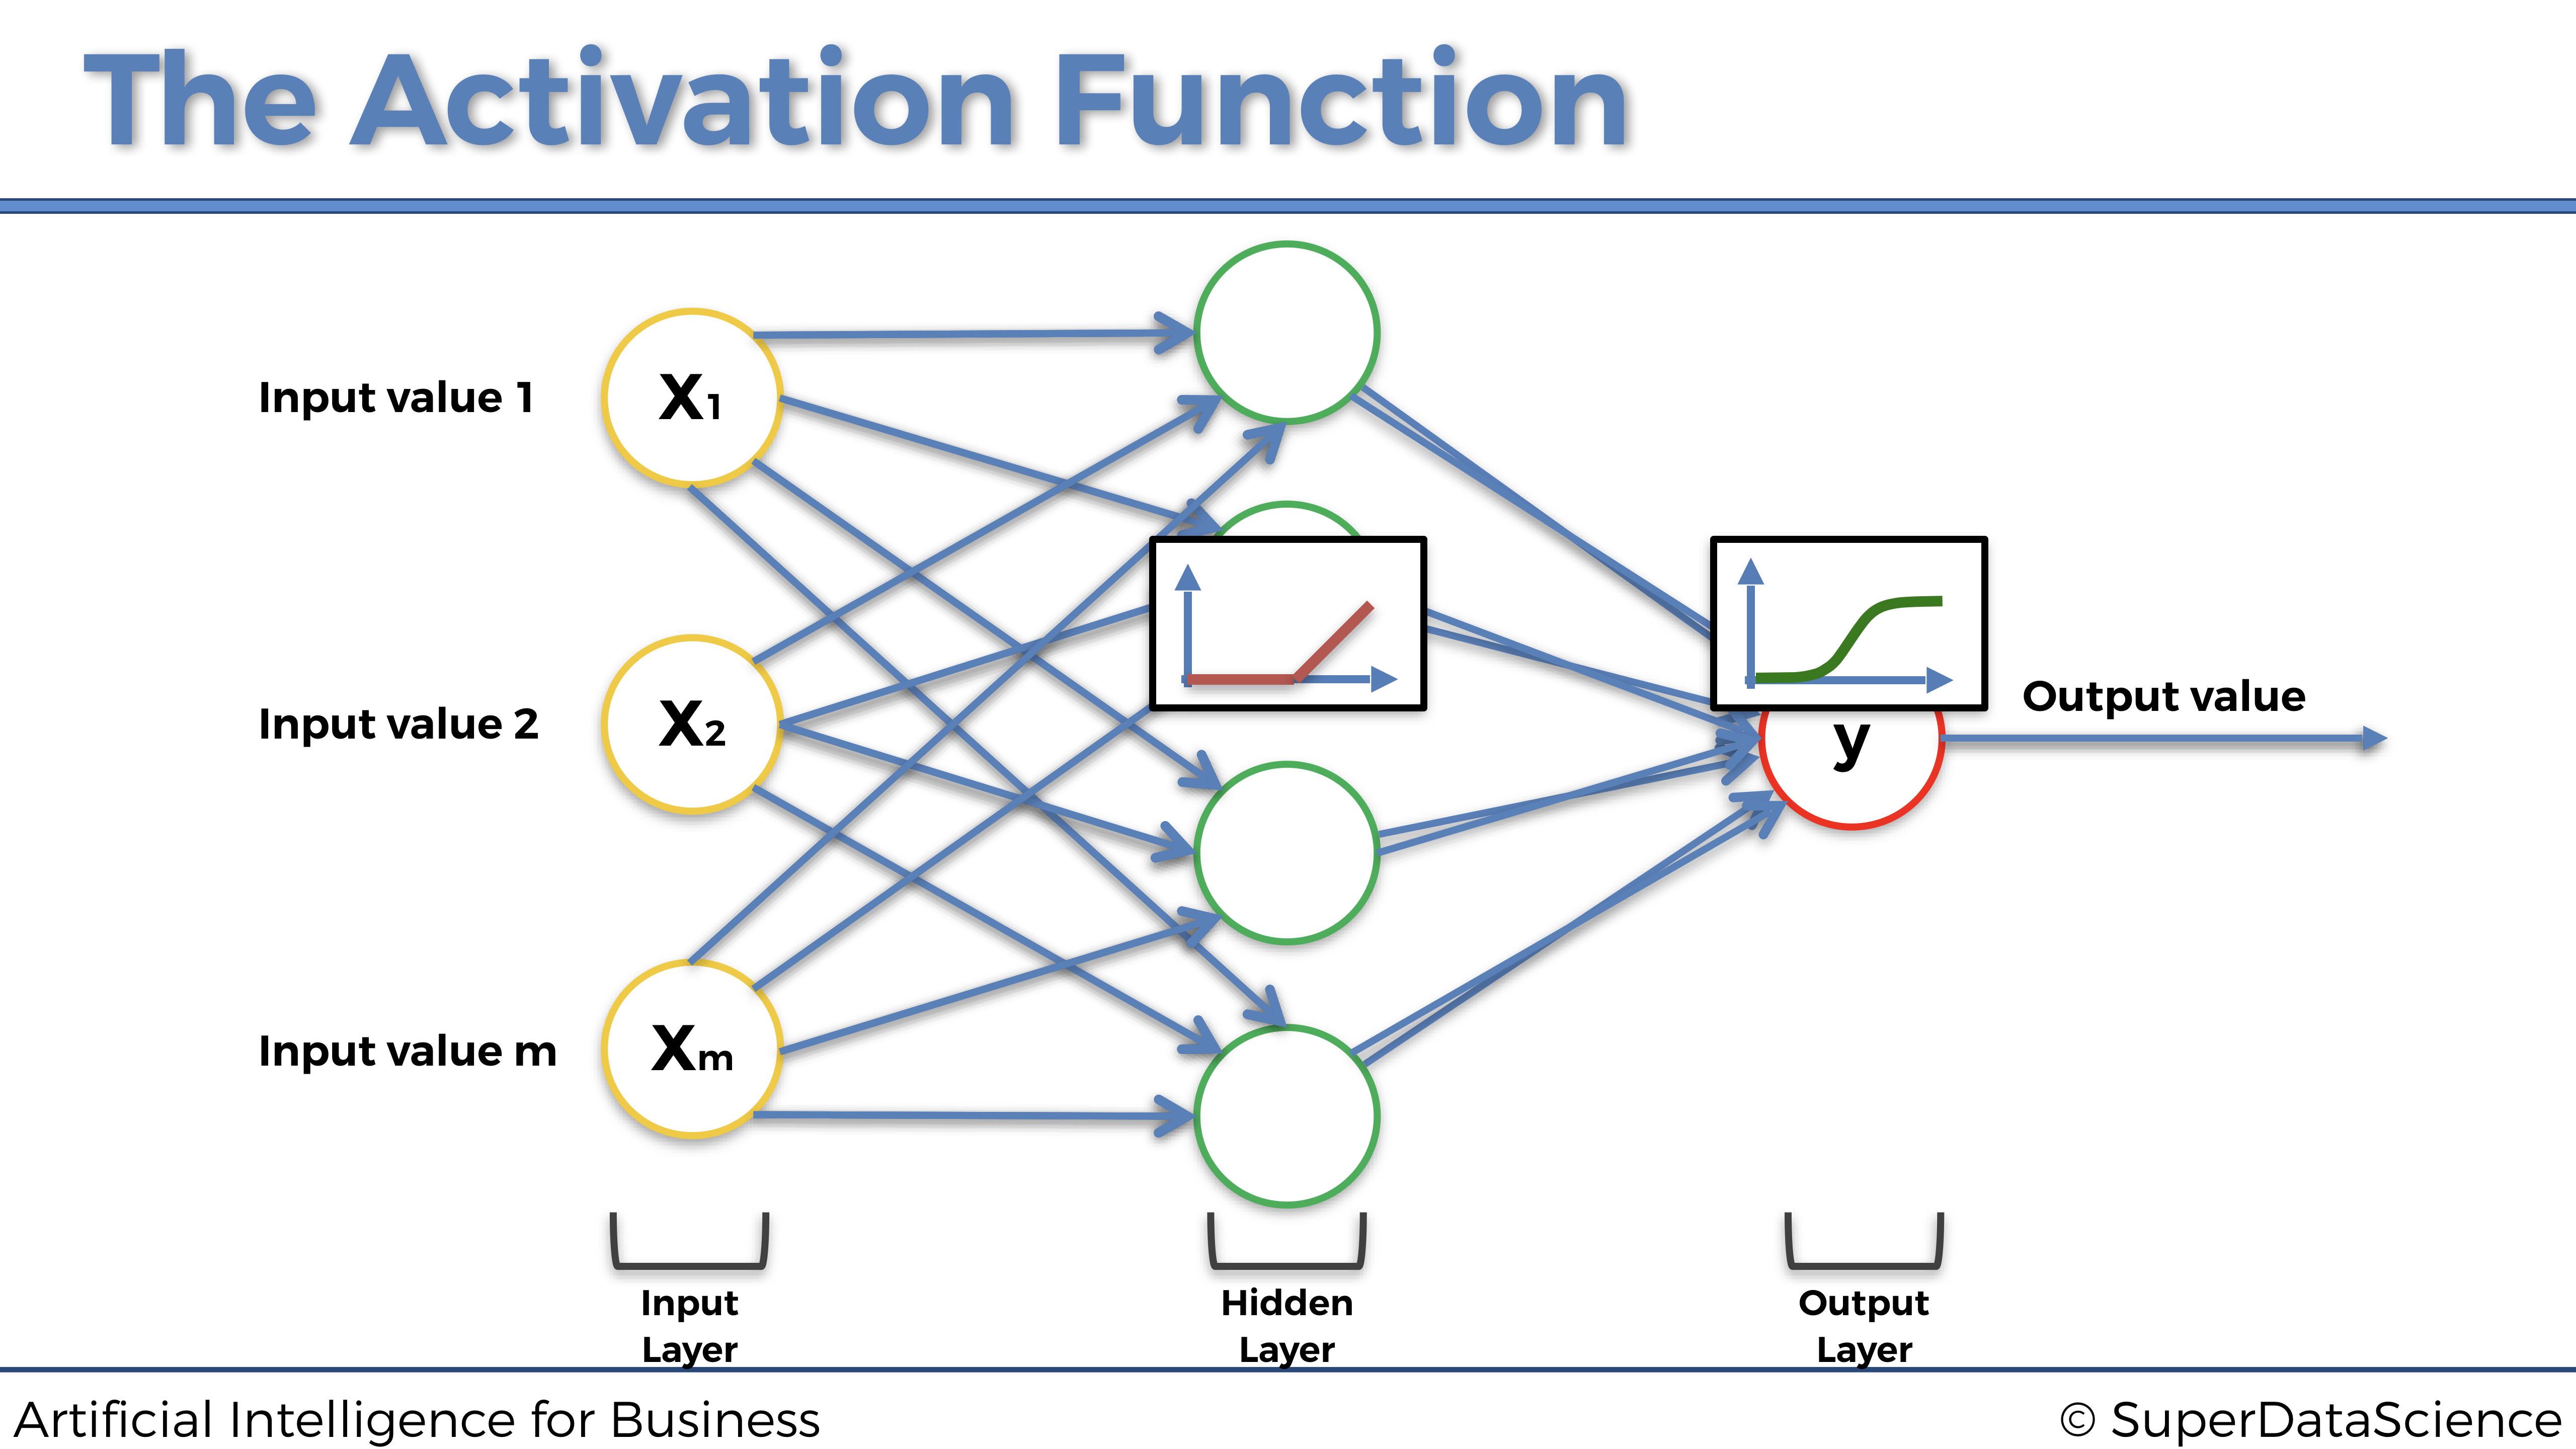
\includegraphics[scale=0.18]{ANN_15.png}
        \end{center}
\end{figure}

And lastly, how to choose between the Rectifier activation function and the Hyperbolic Tangent activation function in the hidden layers? Still easy, you should consider using the Rectifier activation function when the inputs are normalized (scaled between 0 and 1), and the Hyperbolic Tangent activation function when the inputs are standardized (scaled between -1 and +1):

\begin{figure}[!htbp]
        \begin{center}
            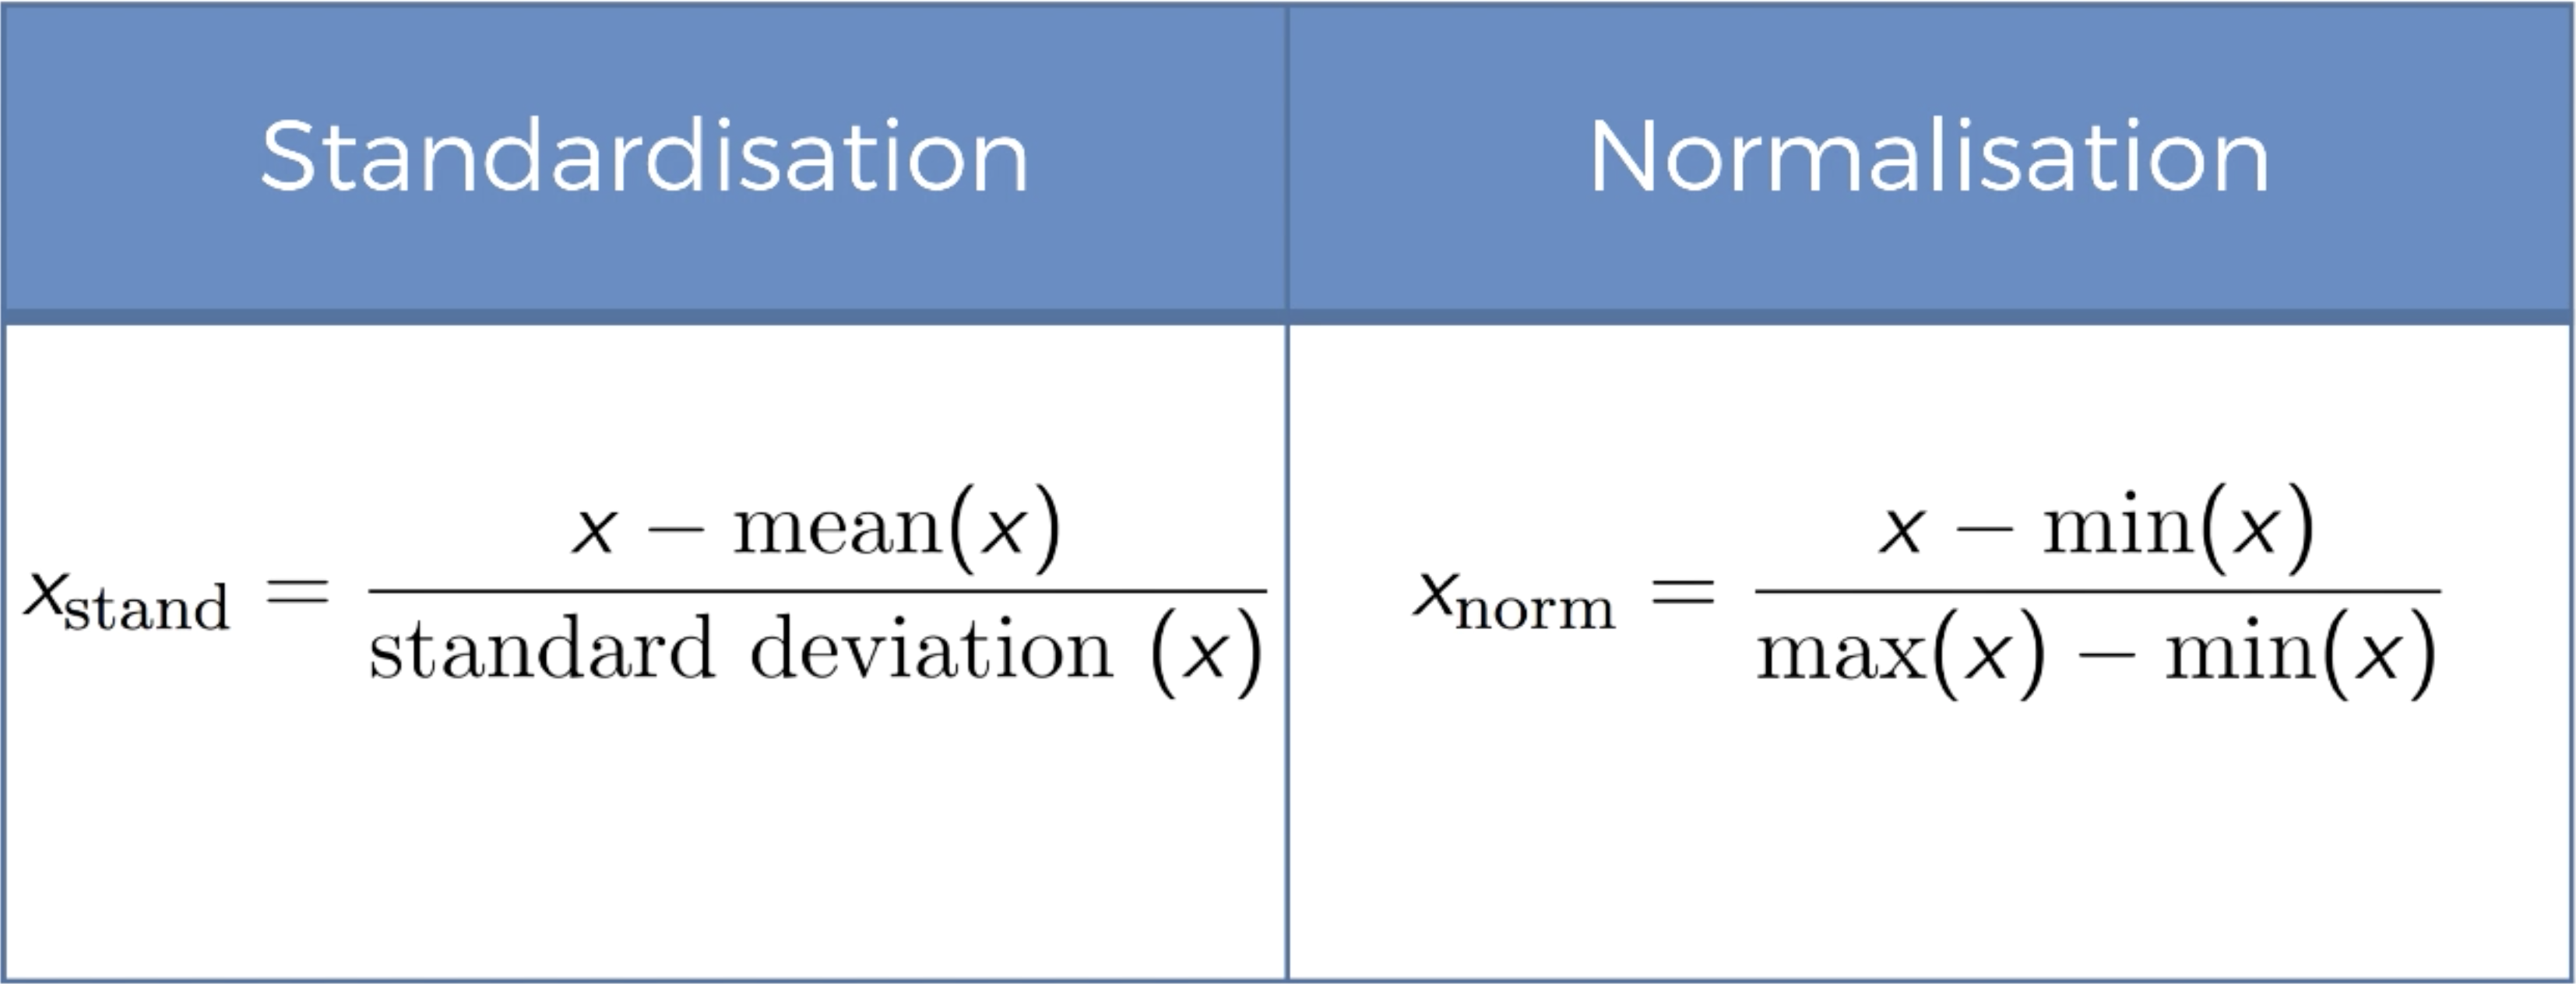
\includegraphics[scale=0.18]{ANN_16.png}
        \end{center}
\end{figure}

Now let's move on to the next section to explain, how Neural Networks work.

\newpage

\subsection{How do Neural Networks work?}

To explain this, let's consider the problem of predicting Real Estate prices. We have some independent variables which we are going to use to predict the price of houses and apartments. For simplicity purpose, and to be able to represent everything in a graph, let's say that our independent variables (our predictors) are the following:

\begin{enumerate}
    \item Area (squared feet)
    \item Number of Bedrooms
    \item Distance to city (Miles)
    \item Age
\end{enumerate}

Then, our dependent variable is of course the apartment price to predict.

Each of the independent variables is attributed a weight, in such a way that the higher is the weight, the more effect the independent variable will have on the dependent variable, that is, the stronger predictor it will be of the dependent variable. Hence, as soon as new inputs enter the Neural Network, the signals are forward-propagated from each of the inputs, reaching the neurons of the hidden layer. Then inside each neuron of the hidden layer, the activation function is applied, so that the lower is the weight of the input, the more the activation function will block the signal coming from that input, and the higher is the weight of that input, the more the activation will let that signal go through. And finally, all the signals coming from the hidden neurons, more or less blocked by the activation functions, are forward propagated to the output layer, to return the final outcome, that is the price prediction.

Let's represent this in the following graphic:

\begin{figure}[!htbp]
        \begin{center}
            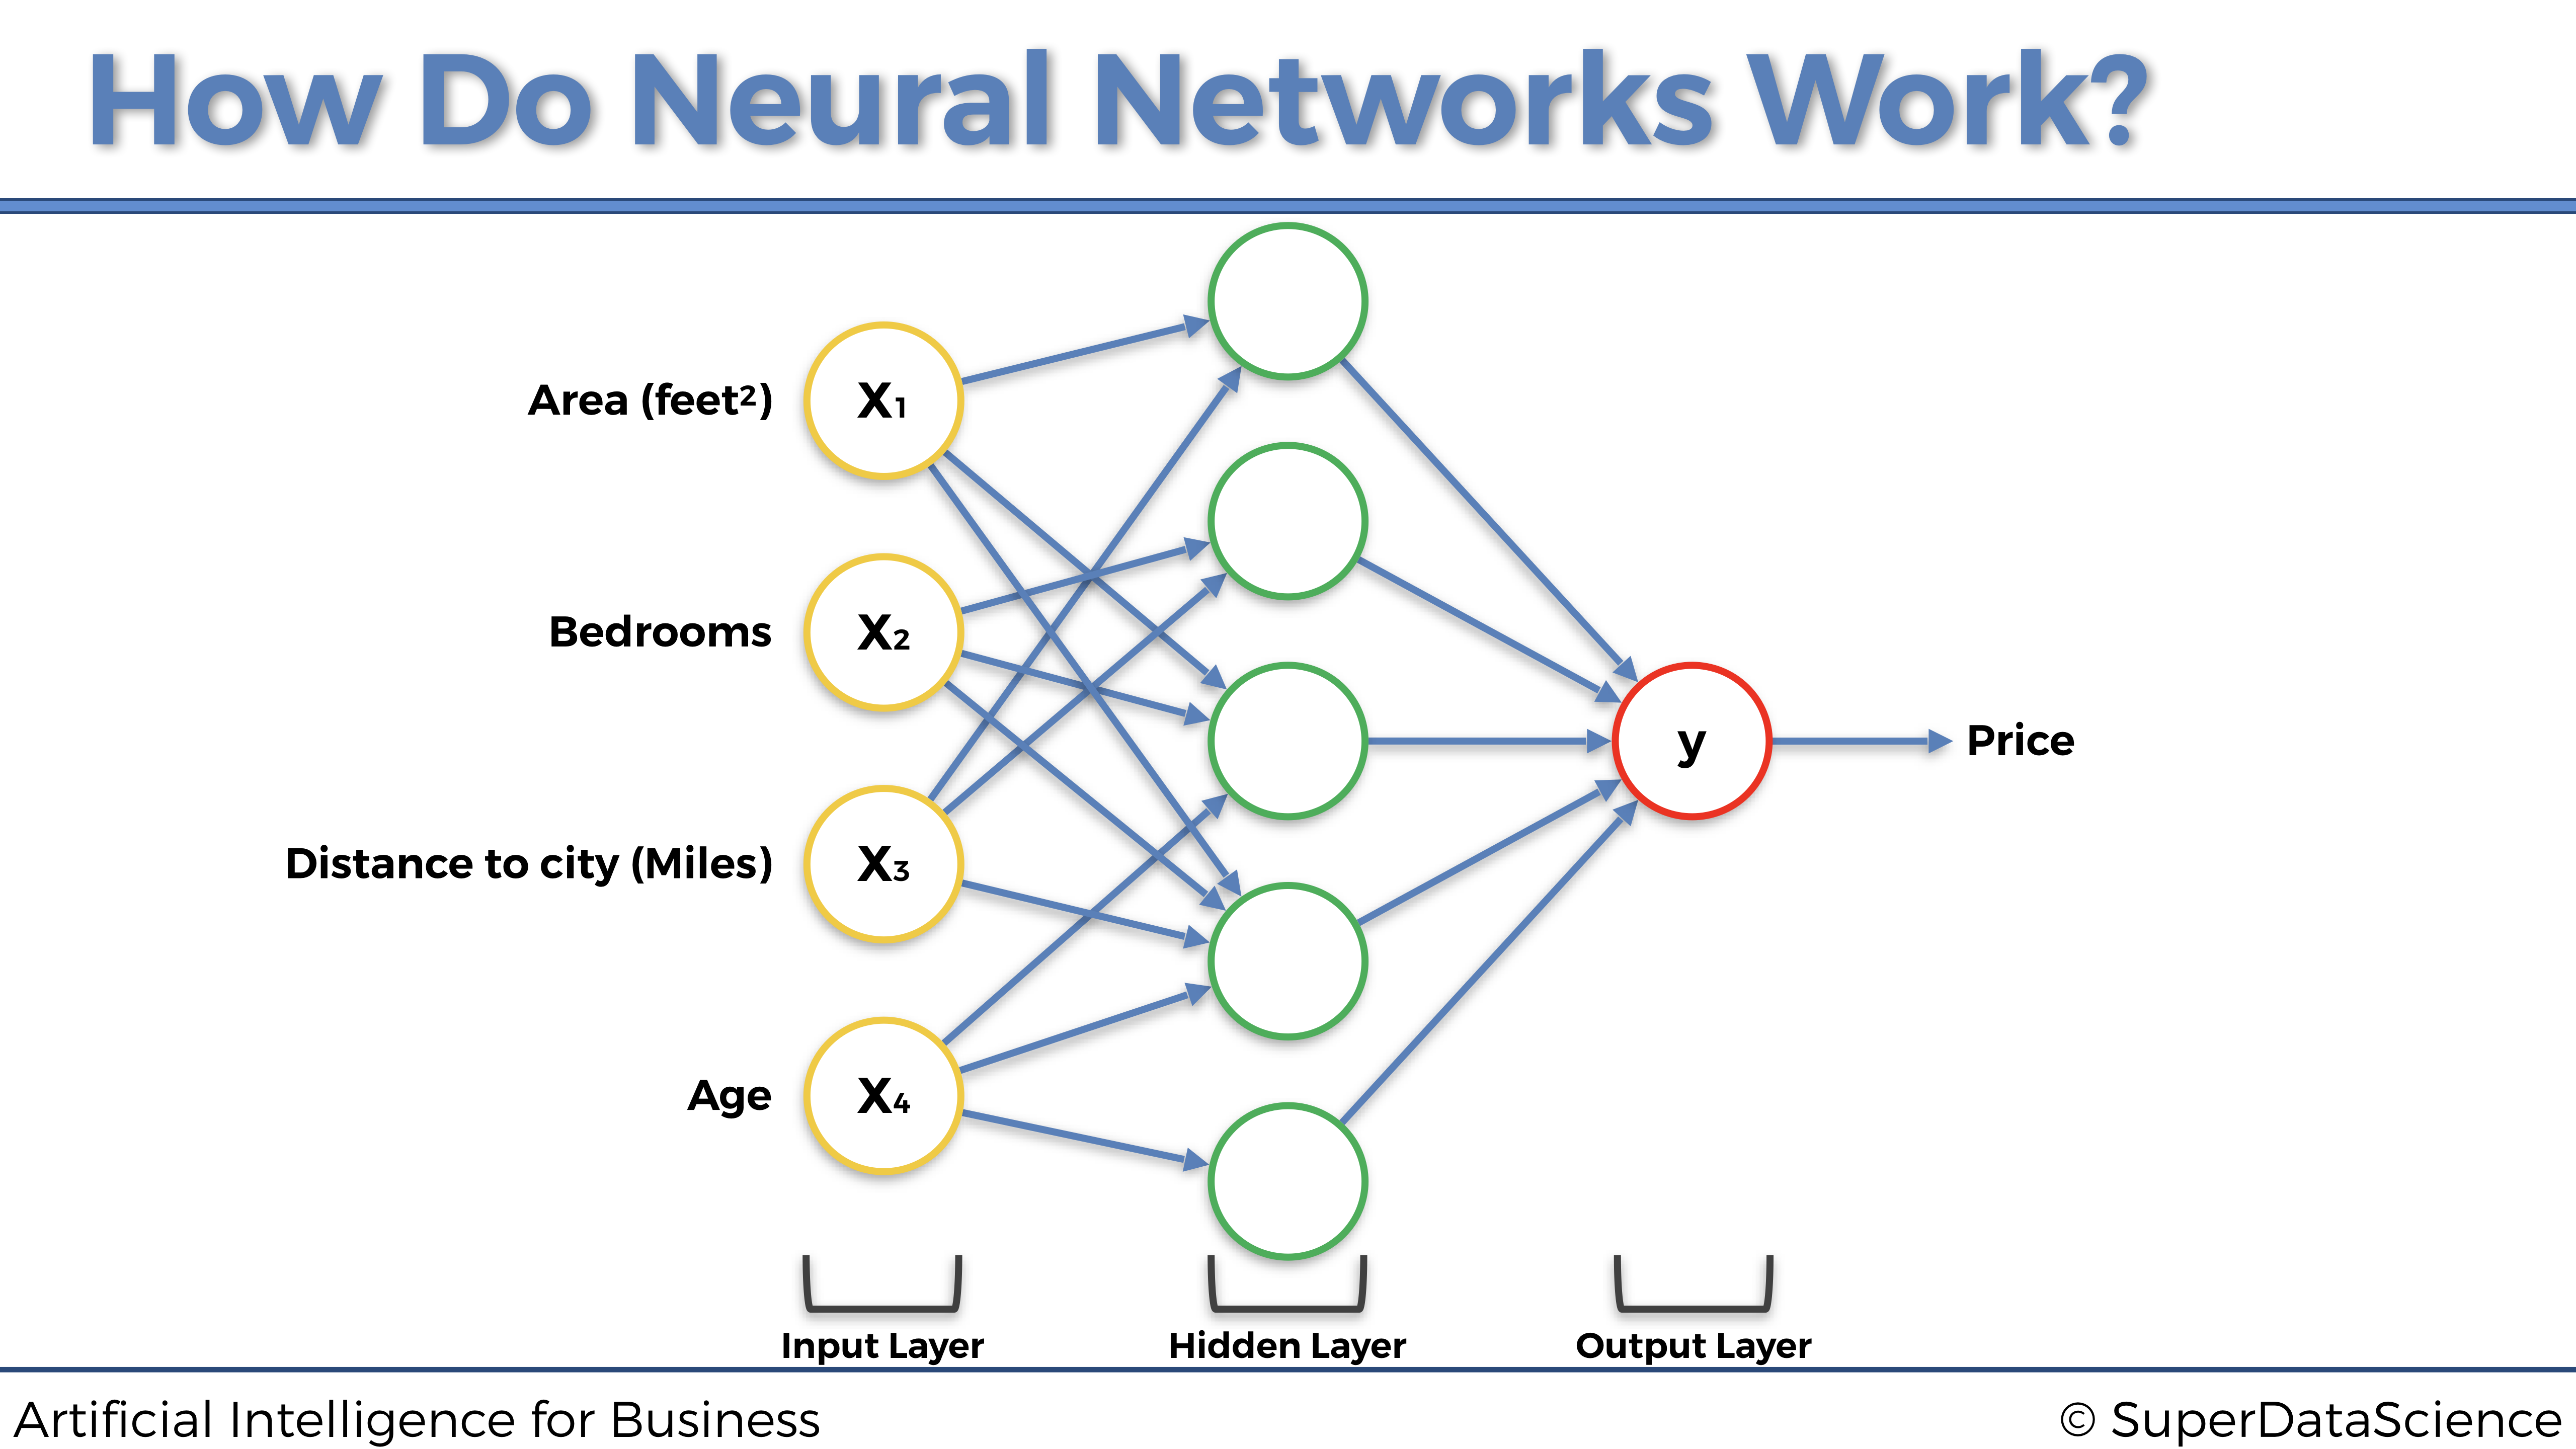
\includegraphics[scale=0.18]{ANN_17.png}
        \end{center}
\end{figure}

\newpage

\subsection{How do Neural Networks learn?}

Simply put, Neural Networks learn by updating, over many iterations, the weights of all the inputs and hidden neurons (when having several hidden layers), towards always the same goal to reduce the loss error between the predictions and the real values.

Indeed, in order for Neural Networks to learn, we need the actual values, which are also called the targets. In our example above about Real Estate Pricing, the actual values are the real prices of the houses and apartments in sales. These real prices depend on the independent variables listed above (area, number of bedrooms, distance to city, and age), and the Neural Network will learn to make better predictions of these prices, by running the following process:

\begin{enumerate}
    \item The Neural Network first forward propagates the signals coming from the input independent variables $x_1$, $x_2$, $x_3$ and $x_4$.
    
    \
    
    \item Then it gets the predicted price $\hat{y}$ in the output layer.
    
    \
    
    \item Then it computes the loss error $C$ between the predicted price $\hat{y}$ (prediction) and the actual price $y$ (target):
    
    \
    
    \begin{equation*}
        C = \frac{1}{2} (\hat{y} - y)^2
    \end{equation*}
    
    \
    
    \item Then this loss error is back-propagated inside the Neural Network, from right to left in our representation.
    
    \
    
    \item Then on each of the neurons the Neural Network runs a technique called Gradient Descent (which we will discuss in the next section), to update the weights into the direction of loss reduction, that is, into new weights which reduce the loss error $C$.
    
    \
    
    \item Then this whole process is repeated many times, with each time new inputs and new targets, until we get the desired performance (early stopping) or the last iteration (number of iterations chosen in the implementation).
\end{enumerate}

Let's represent the two main phases, forward-propagation and back-propagation, of this whole process in the two following separate graphics (see next page):

\newpage

\subsection{Forward-Propagation and Back-Propagation}

\textbf{Phase 1: Forward-Propagation:}

\begin{figure}[!htbp]
        \begin{center}
            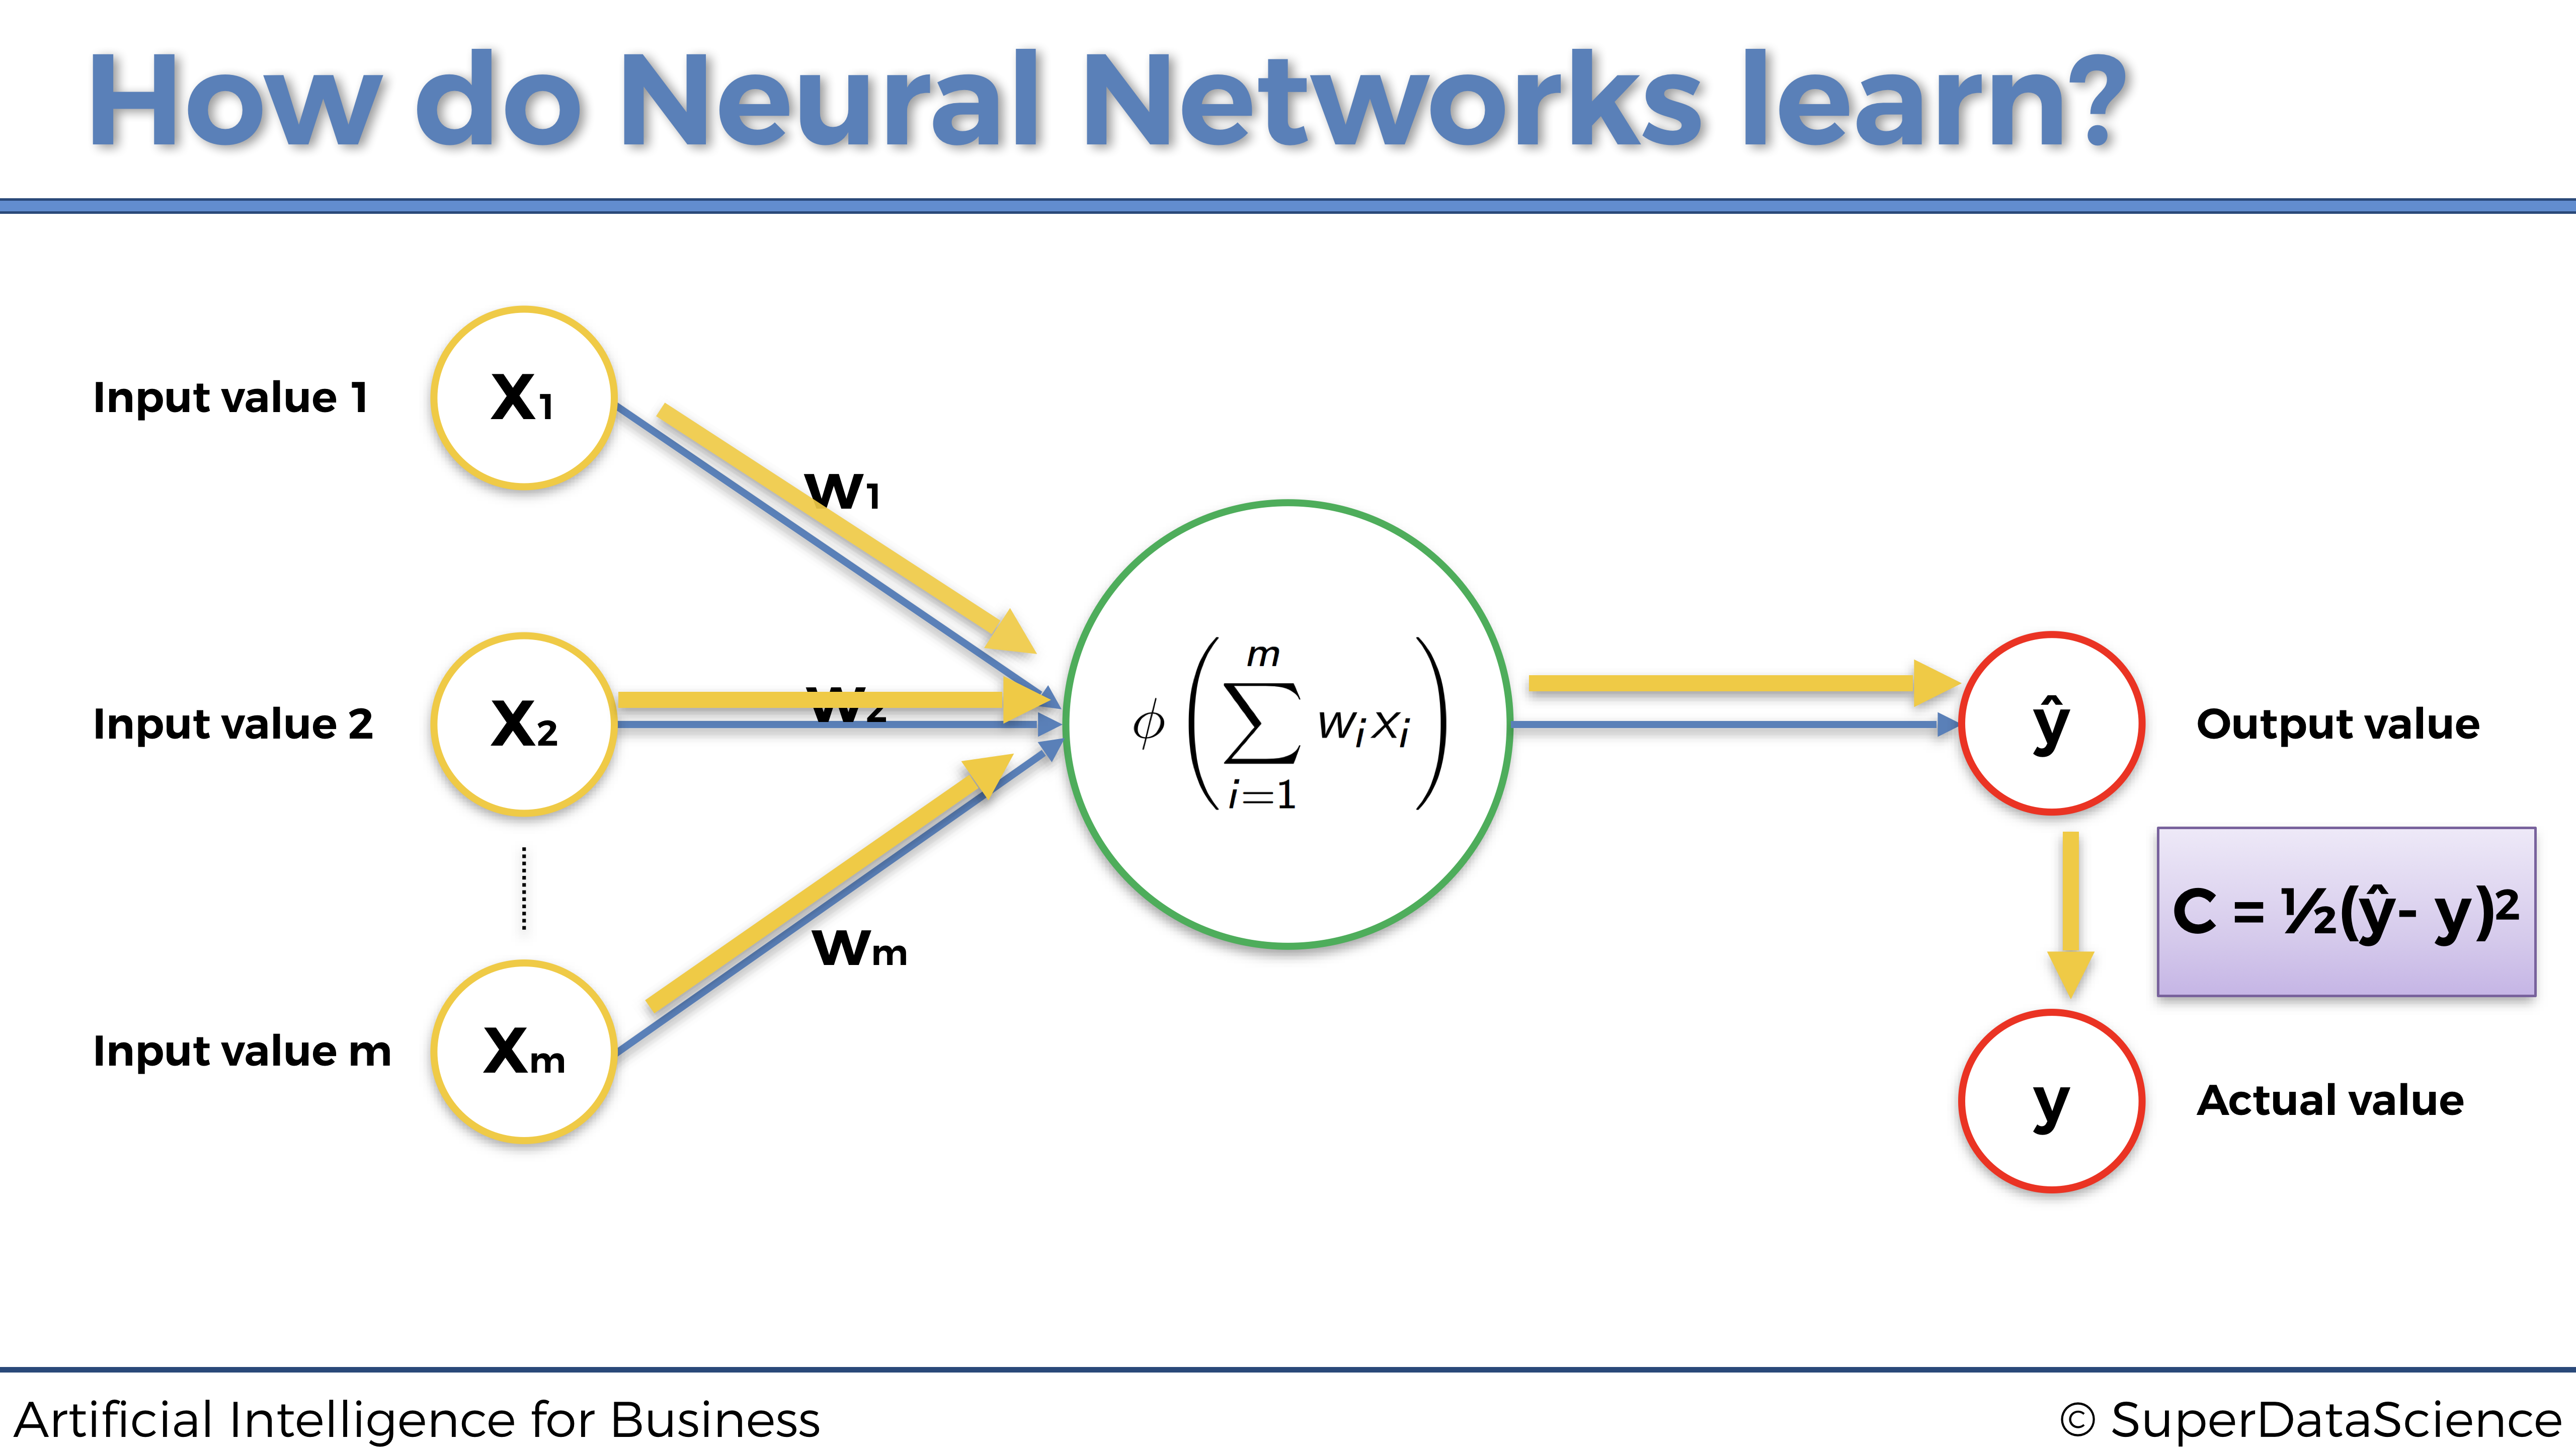
\includegraphics[scale=0.18]{ANN_18.png}
        \end{center}
\end{figure}

\textbf{Phase 2: Back-Propagation:}

\begin{figure}[!htbp]
        \begin{center}
            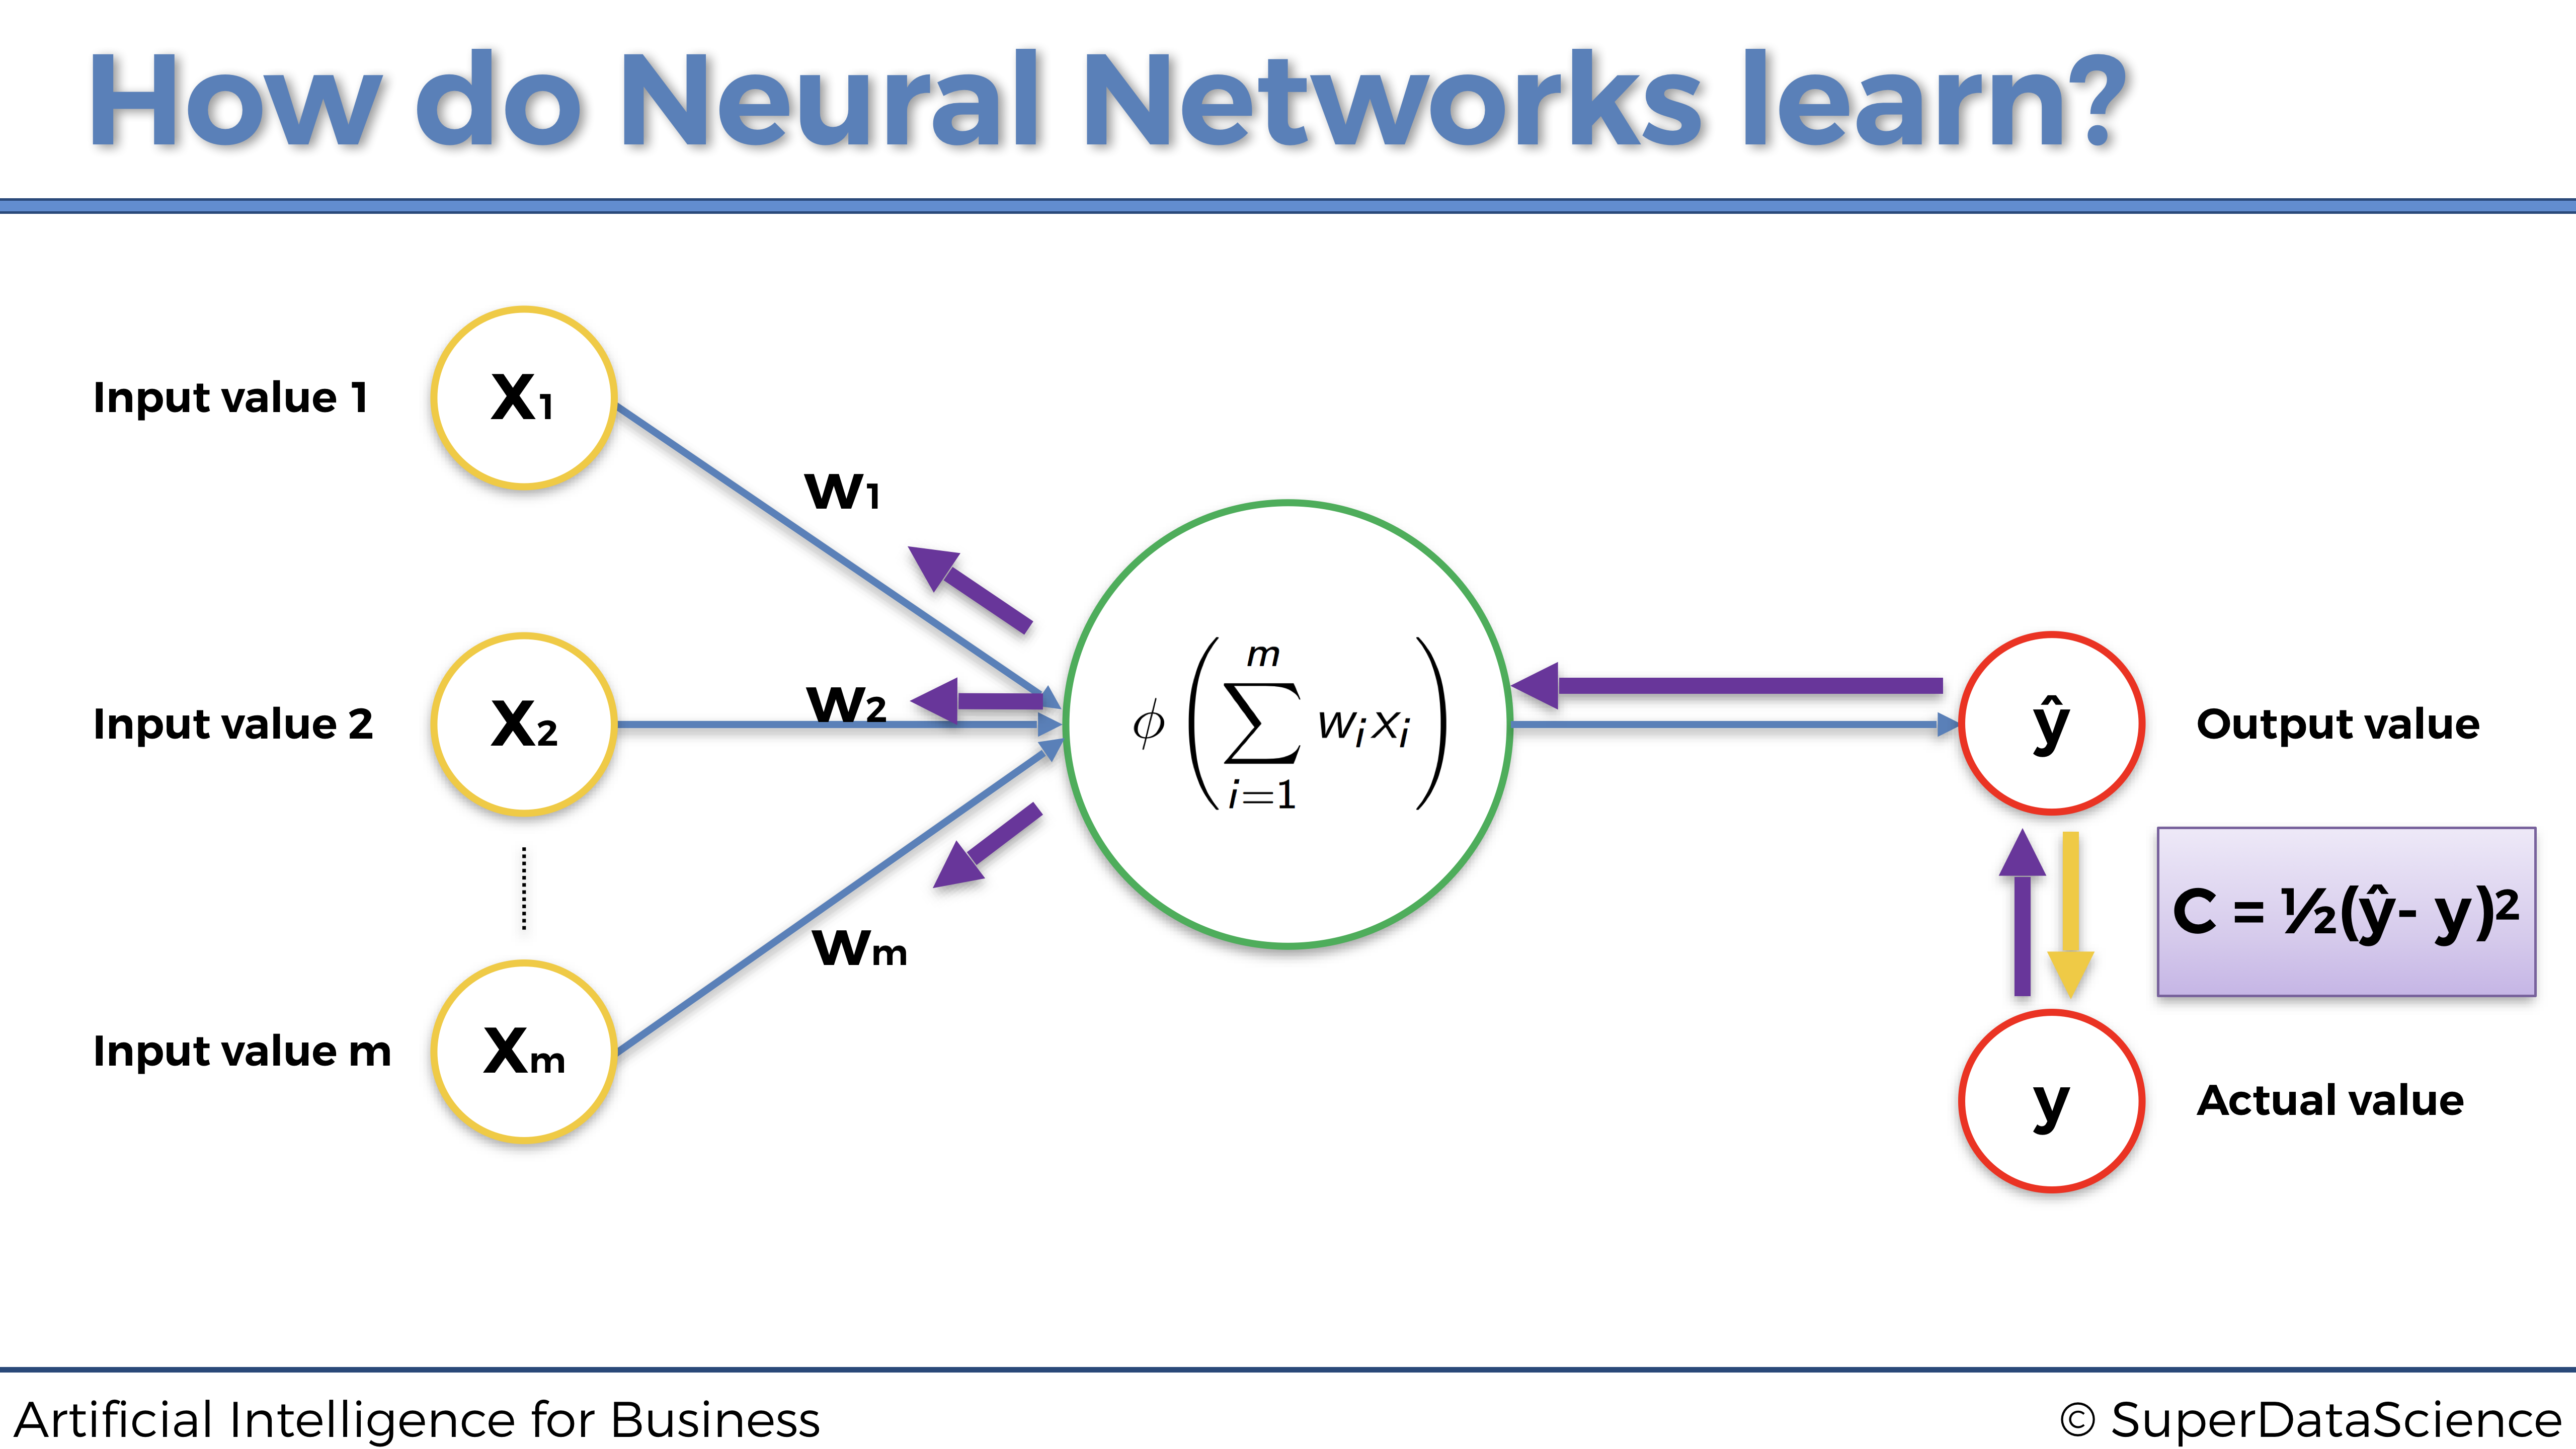
\includegraphics[scale=0.18]{ANN_19.png}
        \end{center}
\end{figure}

\newpage

\subsection{Gradient Descent}

\subsubsection{Gradient Descent Introduction}

When people talk about Machine Learning or Deep Learning they mostly talk about algorithms that are used. But the real questions are, why are those algorithms considered to be Machine Learning or Deep Learning algorithms and others are not? What is the underlining technique that connects them?

The answer to the first question is pretty intuitive: those algorithms are considered to learn their parameters by themselves. This property was not very common before and most algorithms were hand tuned by engineers to achieve a required specification/goal.

But then Gradient Descent came on stage and most algorithms that did not work before suddenly made sense and started to optimize themselves.

So is Gradient Descent magic? Well to someone it is, but for us it is a mathematical algorithm that is used to optimize a model that has its internal parameters (weights). Or, to be more technical, let's see what Wikipedia says about it:

\begin{center}
    “Gradient descent is a first-order iterative optimization algorithm for finding the minimum of a function.”
\end{center}

That is a correct but mouthful definition, and for someone that is just starting, it is the scary one as well! Let's break it down:

\textbf{Algorithm} - In simple words, it is a blueprint on how to solve a problem. Everyday example of an algorithm would be a cooking recipe.

\textbf{Iterative} - This means that it uses some kind of loop (for programmers, for-loops or while-loops) to perform steps. Each step uses previously calculated values as an input for the current step. Now, one question rises, ``What is our initial value?''. We will answer on this a bit later through examples.

\textbf{Optimization} - It tries to find the best solutions according to some criteria leading to several alternative solutions, but only one is consider the best.

\textbf{First-order} - Gradient Descent is using first derivative of a criterion function (cost, loss) in order to find what is a better solution to the given problem.

Hence, when we put everything together in simple words, we get the following:

Gradient descent is a blueprint on how to find the best solution to a problem where more than one solution is acceptable. It uses a goal to determine how far we are from finding the best solution.

Until this point we have everything clarified except the cost function.

The cost is the indicator that we follow during the optimization process. Based on that indicator we can tell how far we are from the optimum of a function. One good example of the Cost is the Mean-Squared Error, which we have seen earlier in this book:

\begin{equation*}
    \textrm{MSE} = \frac{1}{n} \sum_{i=1}^n (y_i - \hat{y}_i)
\end{equation*}

where:

\begin{equation*}
    \begin{cases}
        \textrm{$\hat{y}_i$ is the model prediction} \\
        \textrm{$y_i$ is the target (the actual value)} \\
        \textrm{$n$ is the number of samples in a dataset}
    \end{cases}
\end{equation*}

Every algorithm that uses Gradient Descent as an optimization technique has parameters (weights) which are changing during the optimization process. When we say that we are looking for the minimum of the loss function, we actually mean we are looking for the values of the weights for which the loss has the lowest possible value.

Accordingly, to answer our second question from the beginning, the technique that connects all the Machine Learning algorithms from Linear Regression to the most complicated neural networks is indeed, Gradient Descent.

\subsubsection{Gradient Descent Intuition}

As we have seen, Gradient Descent is an optimization technique that helps us find the minimum of a cost function. Now let's visualize it in the most intuitive way, like the following ball in a bowl (with little math sprinkle on top of it):

\begin{figure}[!htbp]
        \begin{center}
            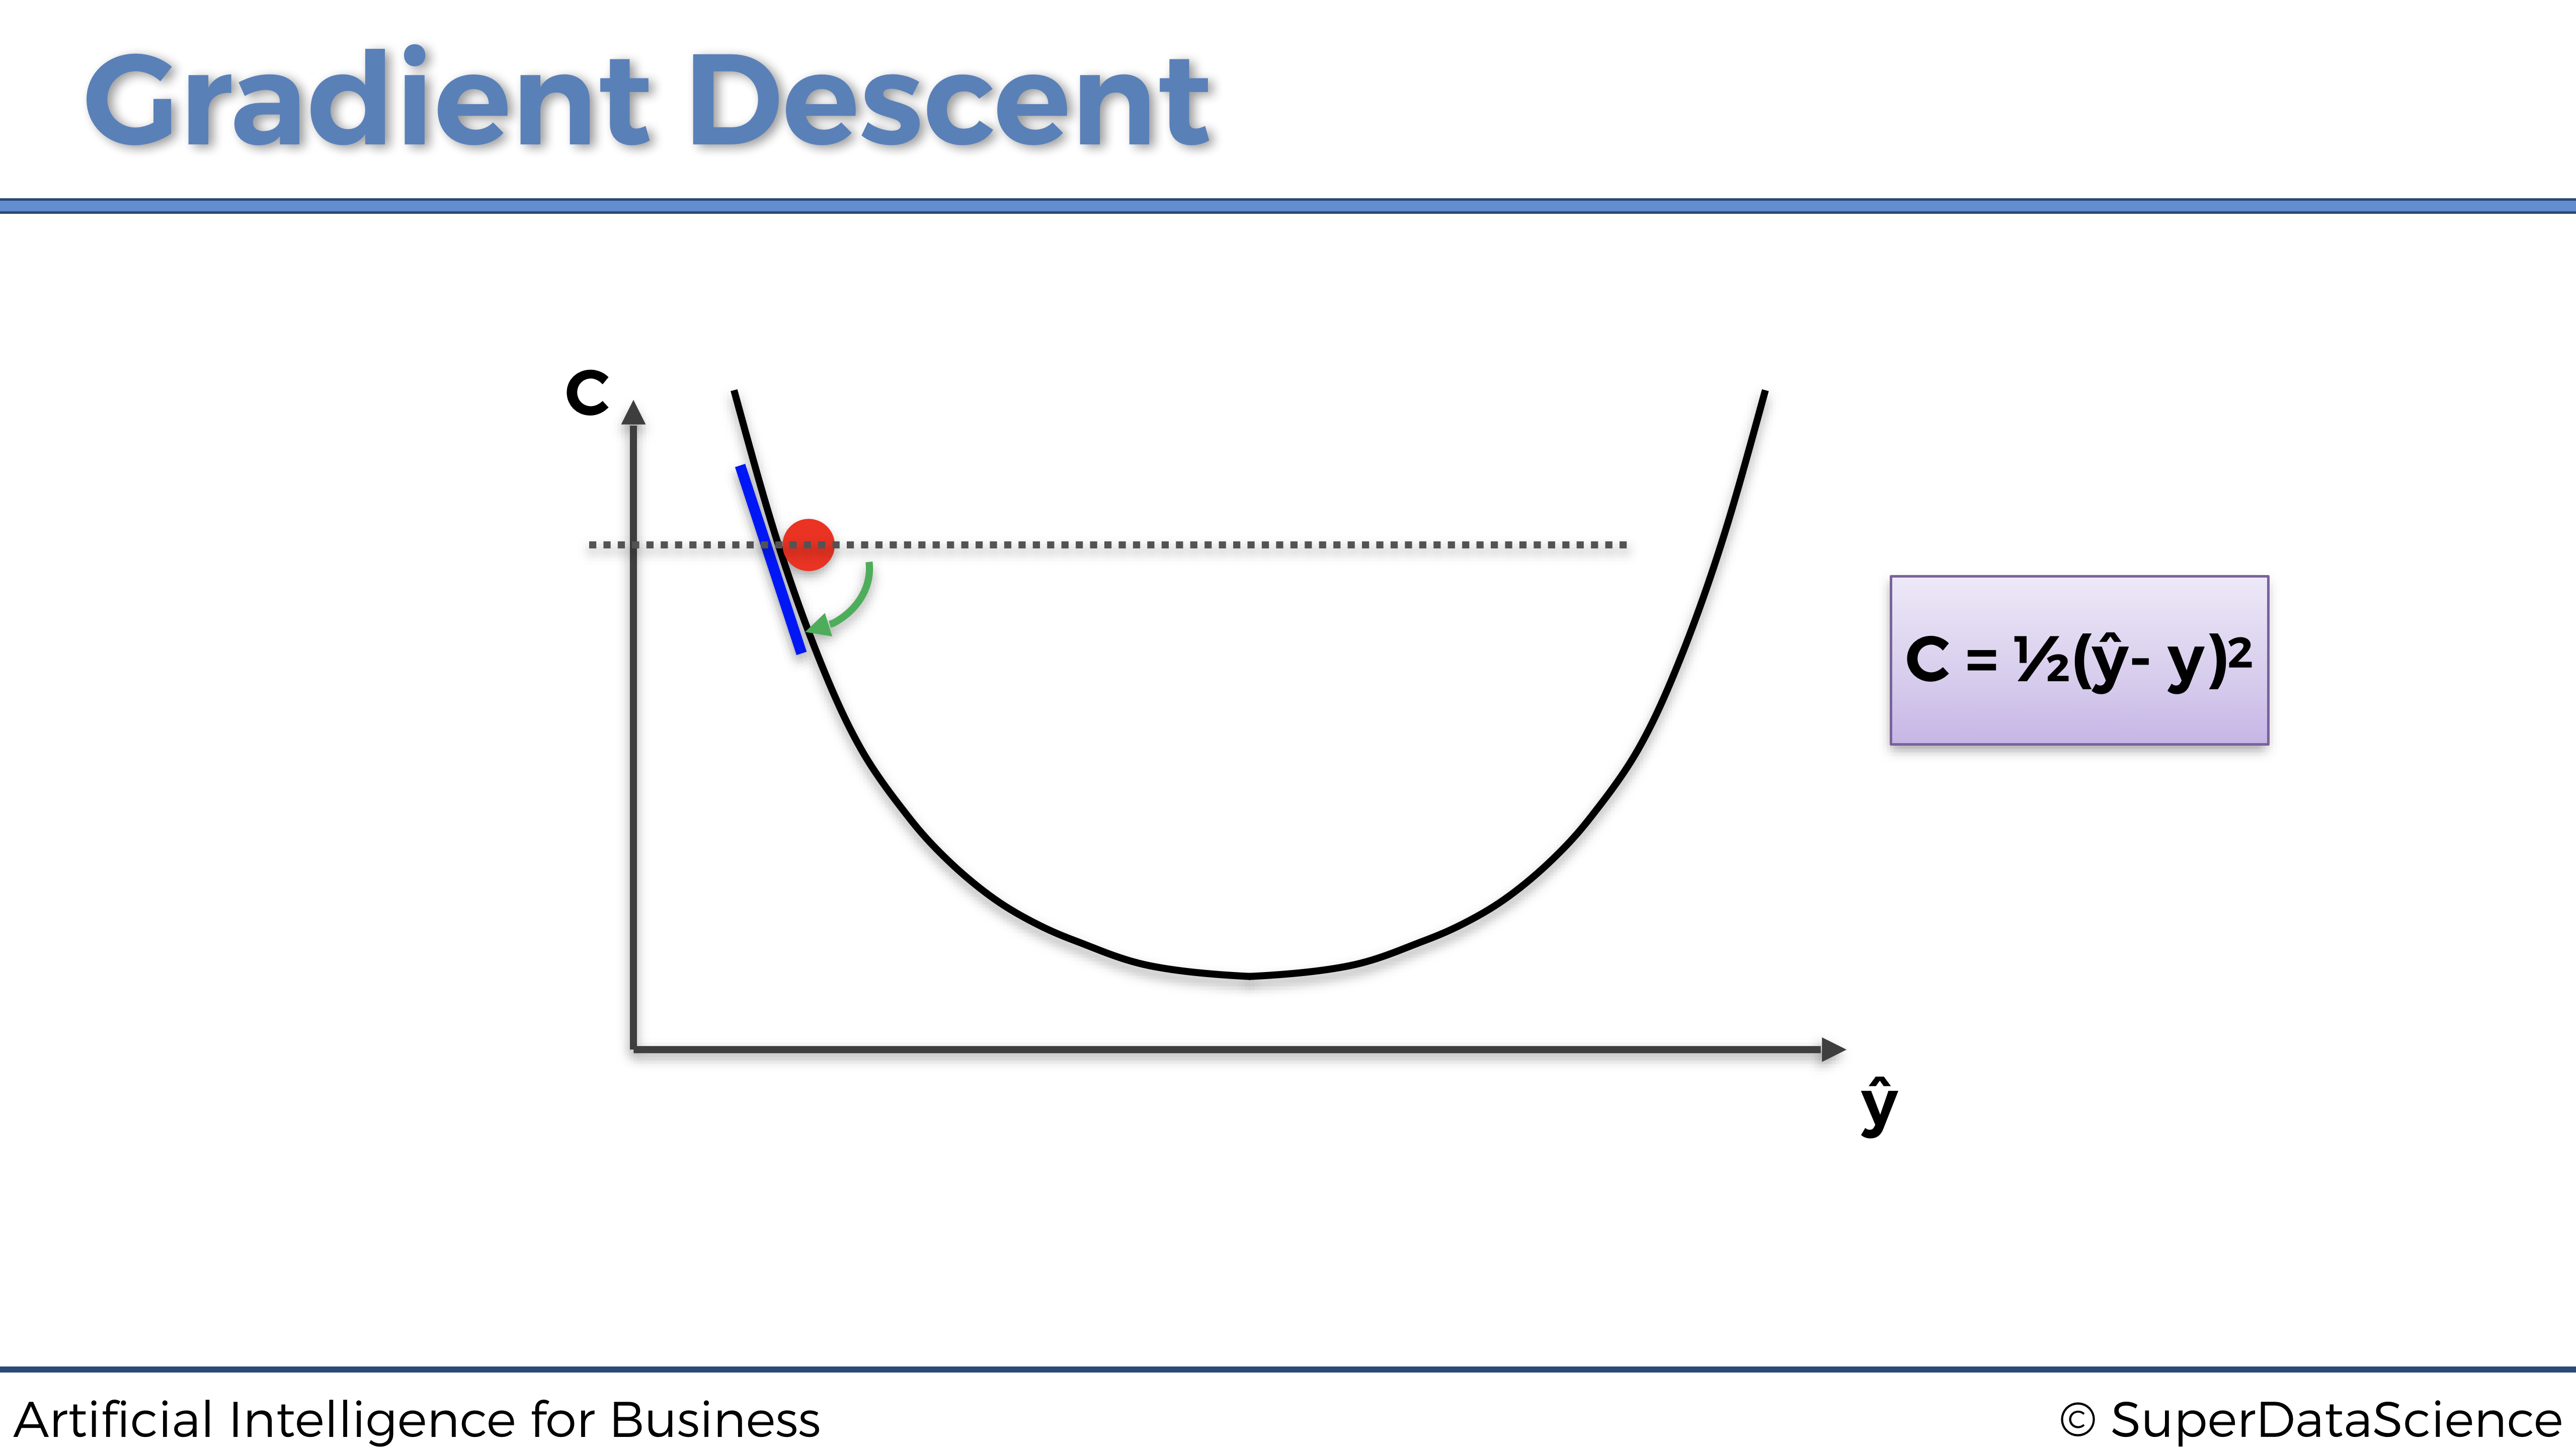
\includegraphics[scale=0.18]{ANN_20.png}
        \end{center}
\end{figure}

Imagine this is a cross section of a bowl, inside which we drop a small red ball and let it find its way down to the bottom of the bowl. After some time it will stop rolling since it has found the sweet spot for it, at the bottom of the bowl.

You can think about the Gradient Descent in the same way. It starts somewhere in the bowl (initial values of parameters) and tries to find the bottom of the bowl, or in other words, the minimum of a cost function.

Let's go through the example that is shown on the image above. The initial values of the parameters have set our ball at the position shown. Based on that we get some predictions, which we compare to our target values. The difference between these two sets will be our loss for the current set of parameters.

Then we calculate the first derivative of the cost function, with respect to the parameters. This is where the name \textbf{Gradient} comes from. Here, this first derivative gives us the slope of the tangent to the curve where the ball is. If the slope is negative, like on the picture above, we take the next step to the right side. If the slope is positive we take the next step to the left side.

The name \textbf{Descent} thus comes from the fact that we always take the next step that points downhill, as represented in the following graphic:

\begin{figure}[!htbp]
        \begin{center}
            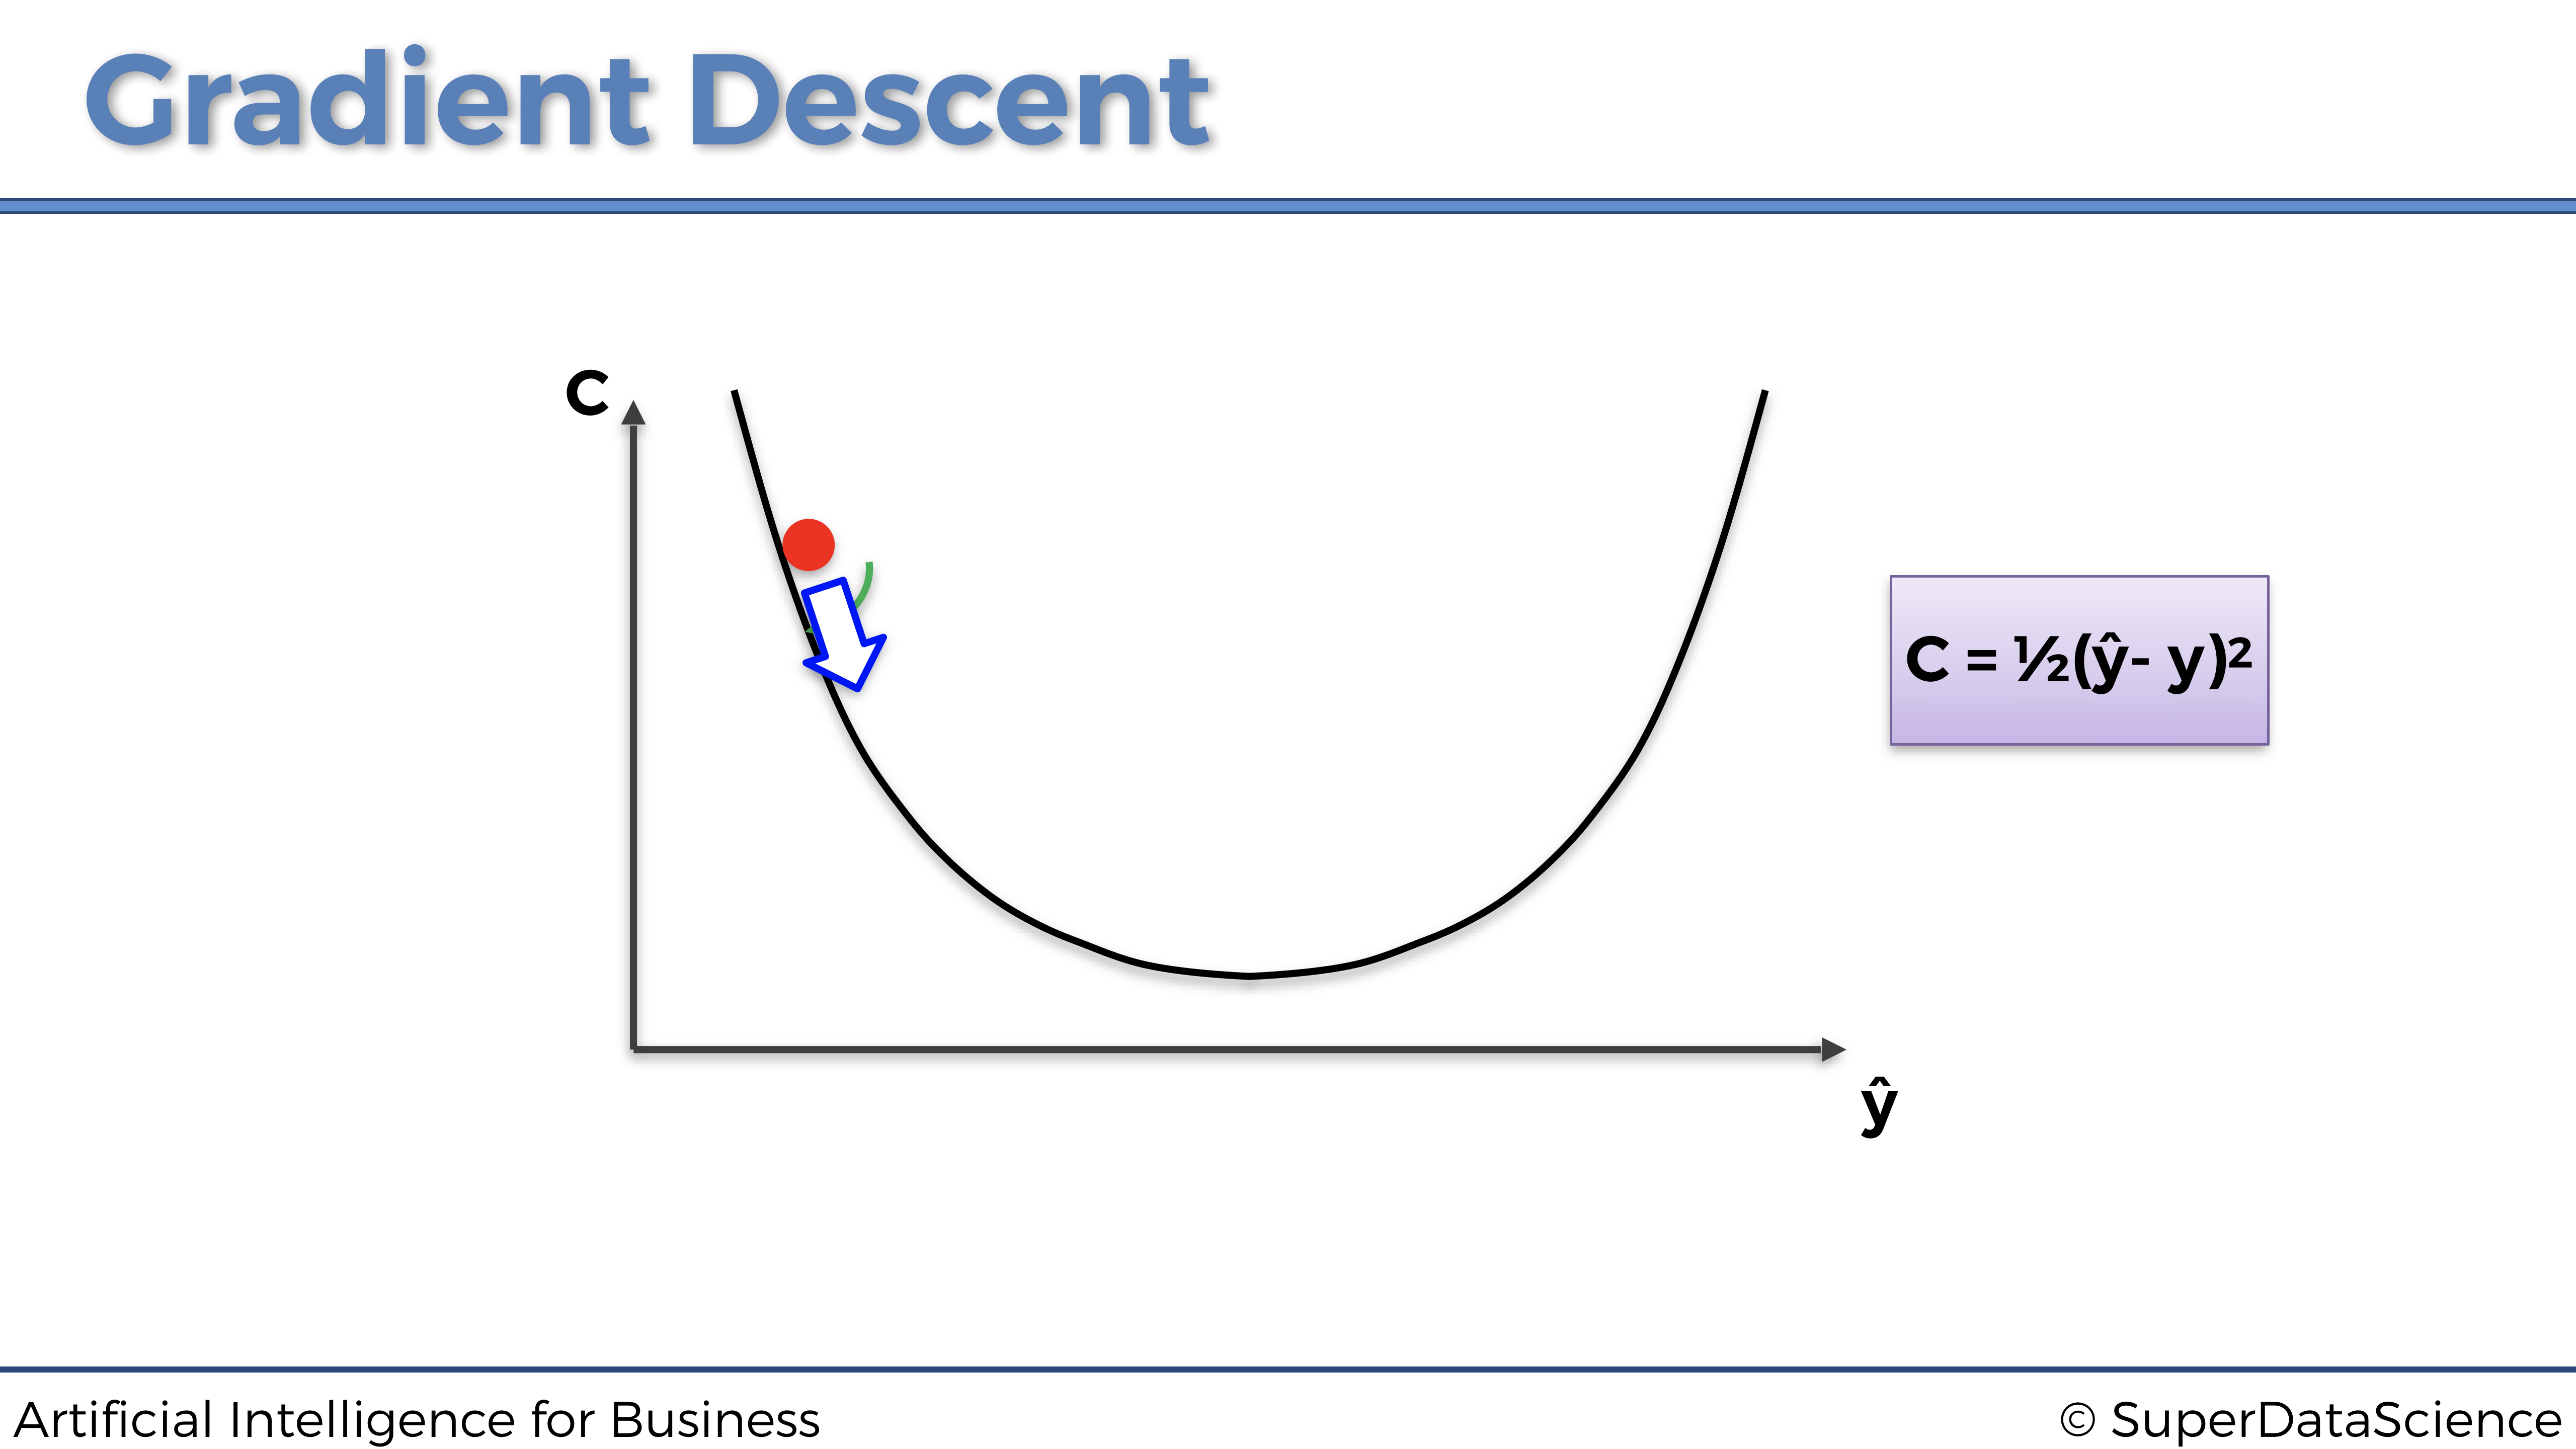
\includegraphics[scale=0.15]{ANN_21.png}
        \end{center}
\end{figure}

Now at this position our ball has a positive slope, so we have to take the next step to the left.

\begin{figure}[!htbp]
        \begin{center}
            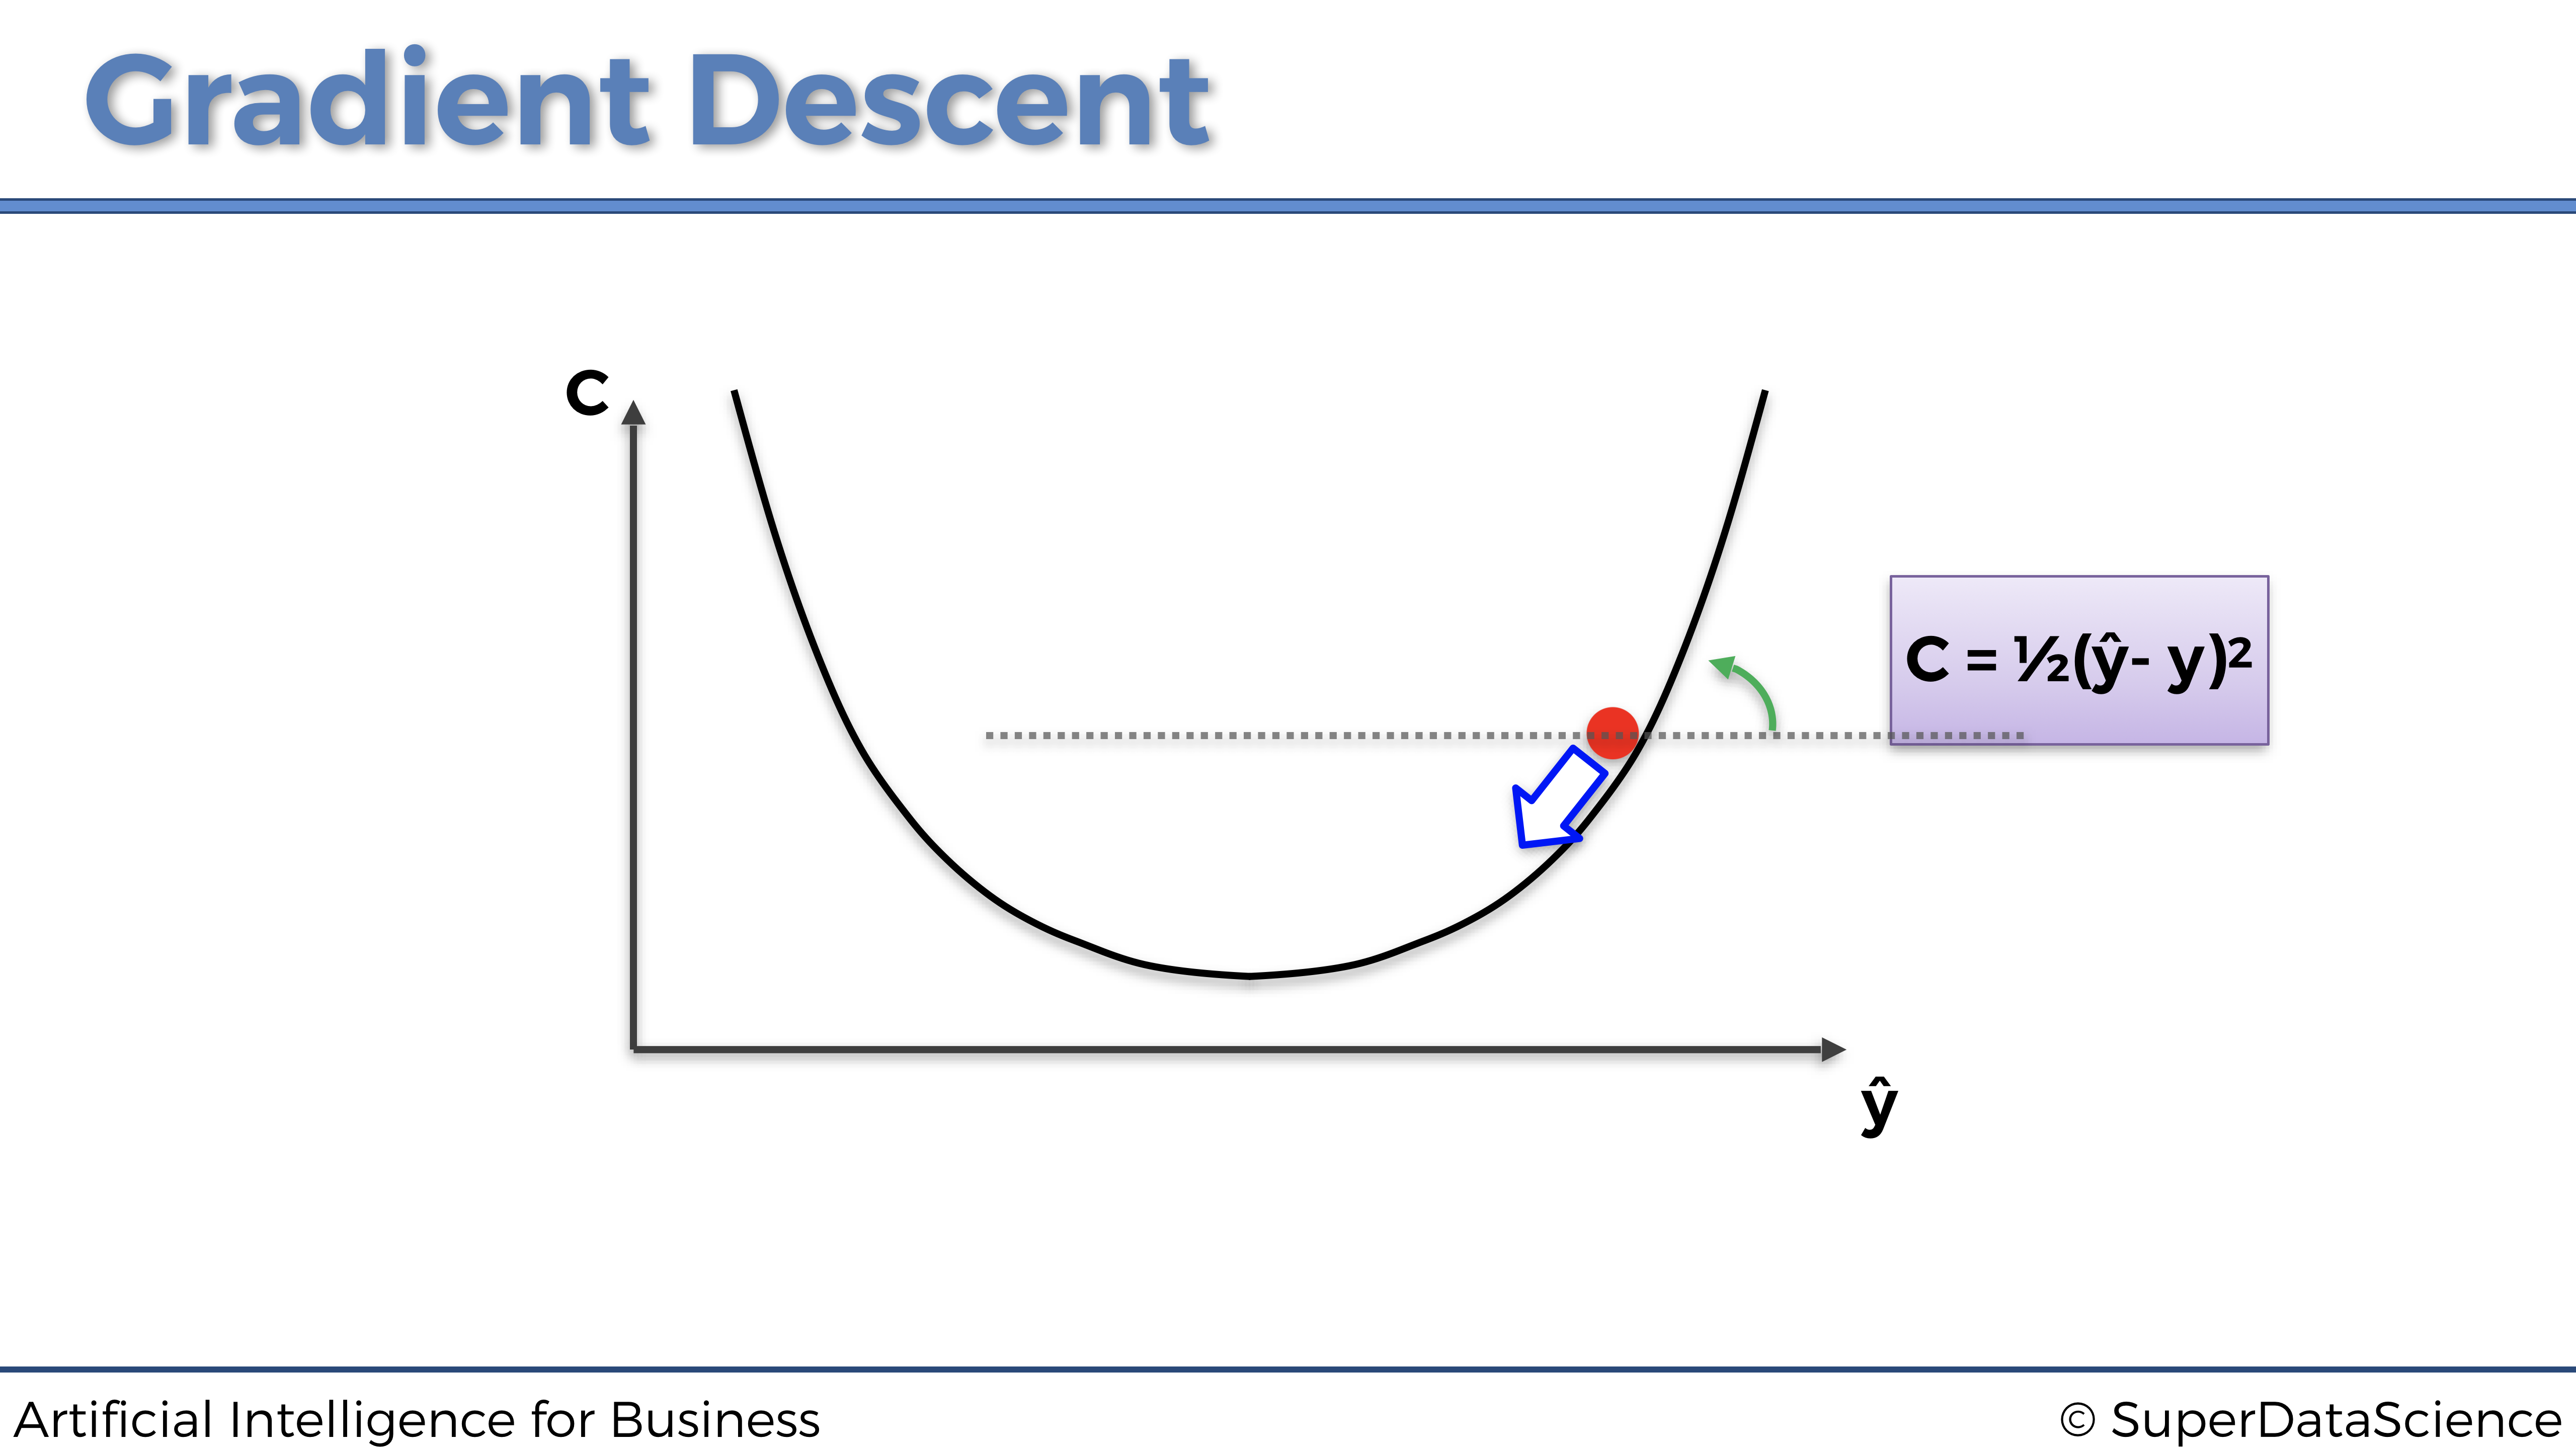
\includegraphics[scale=0.15]{ANN_22.png}
        \end{center}
\end{figure}

Eventually, by repeating the same steps, the ball will end up at the bottom of the bowl:

\begin{figure}[!htbp]
        \begin{center}
            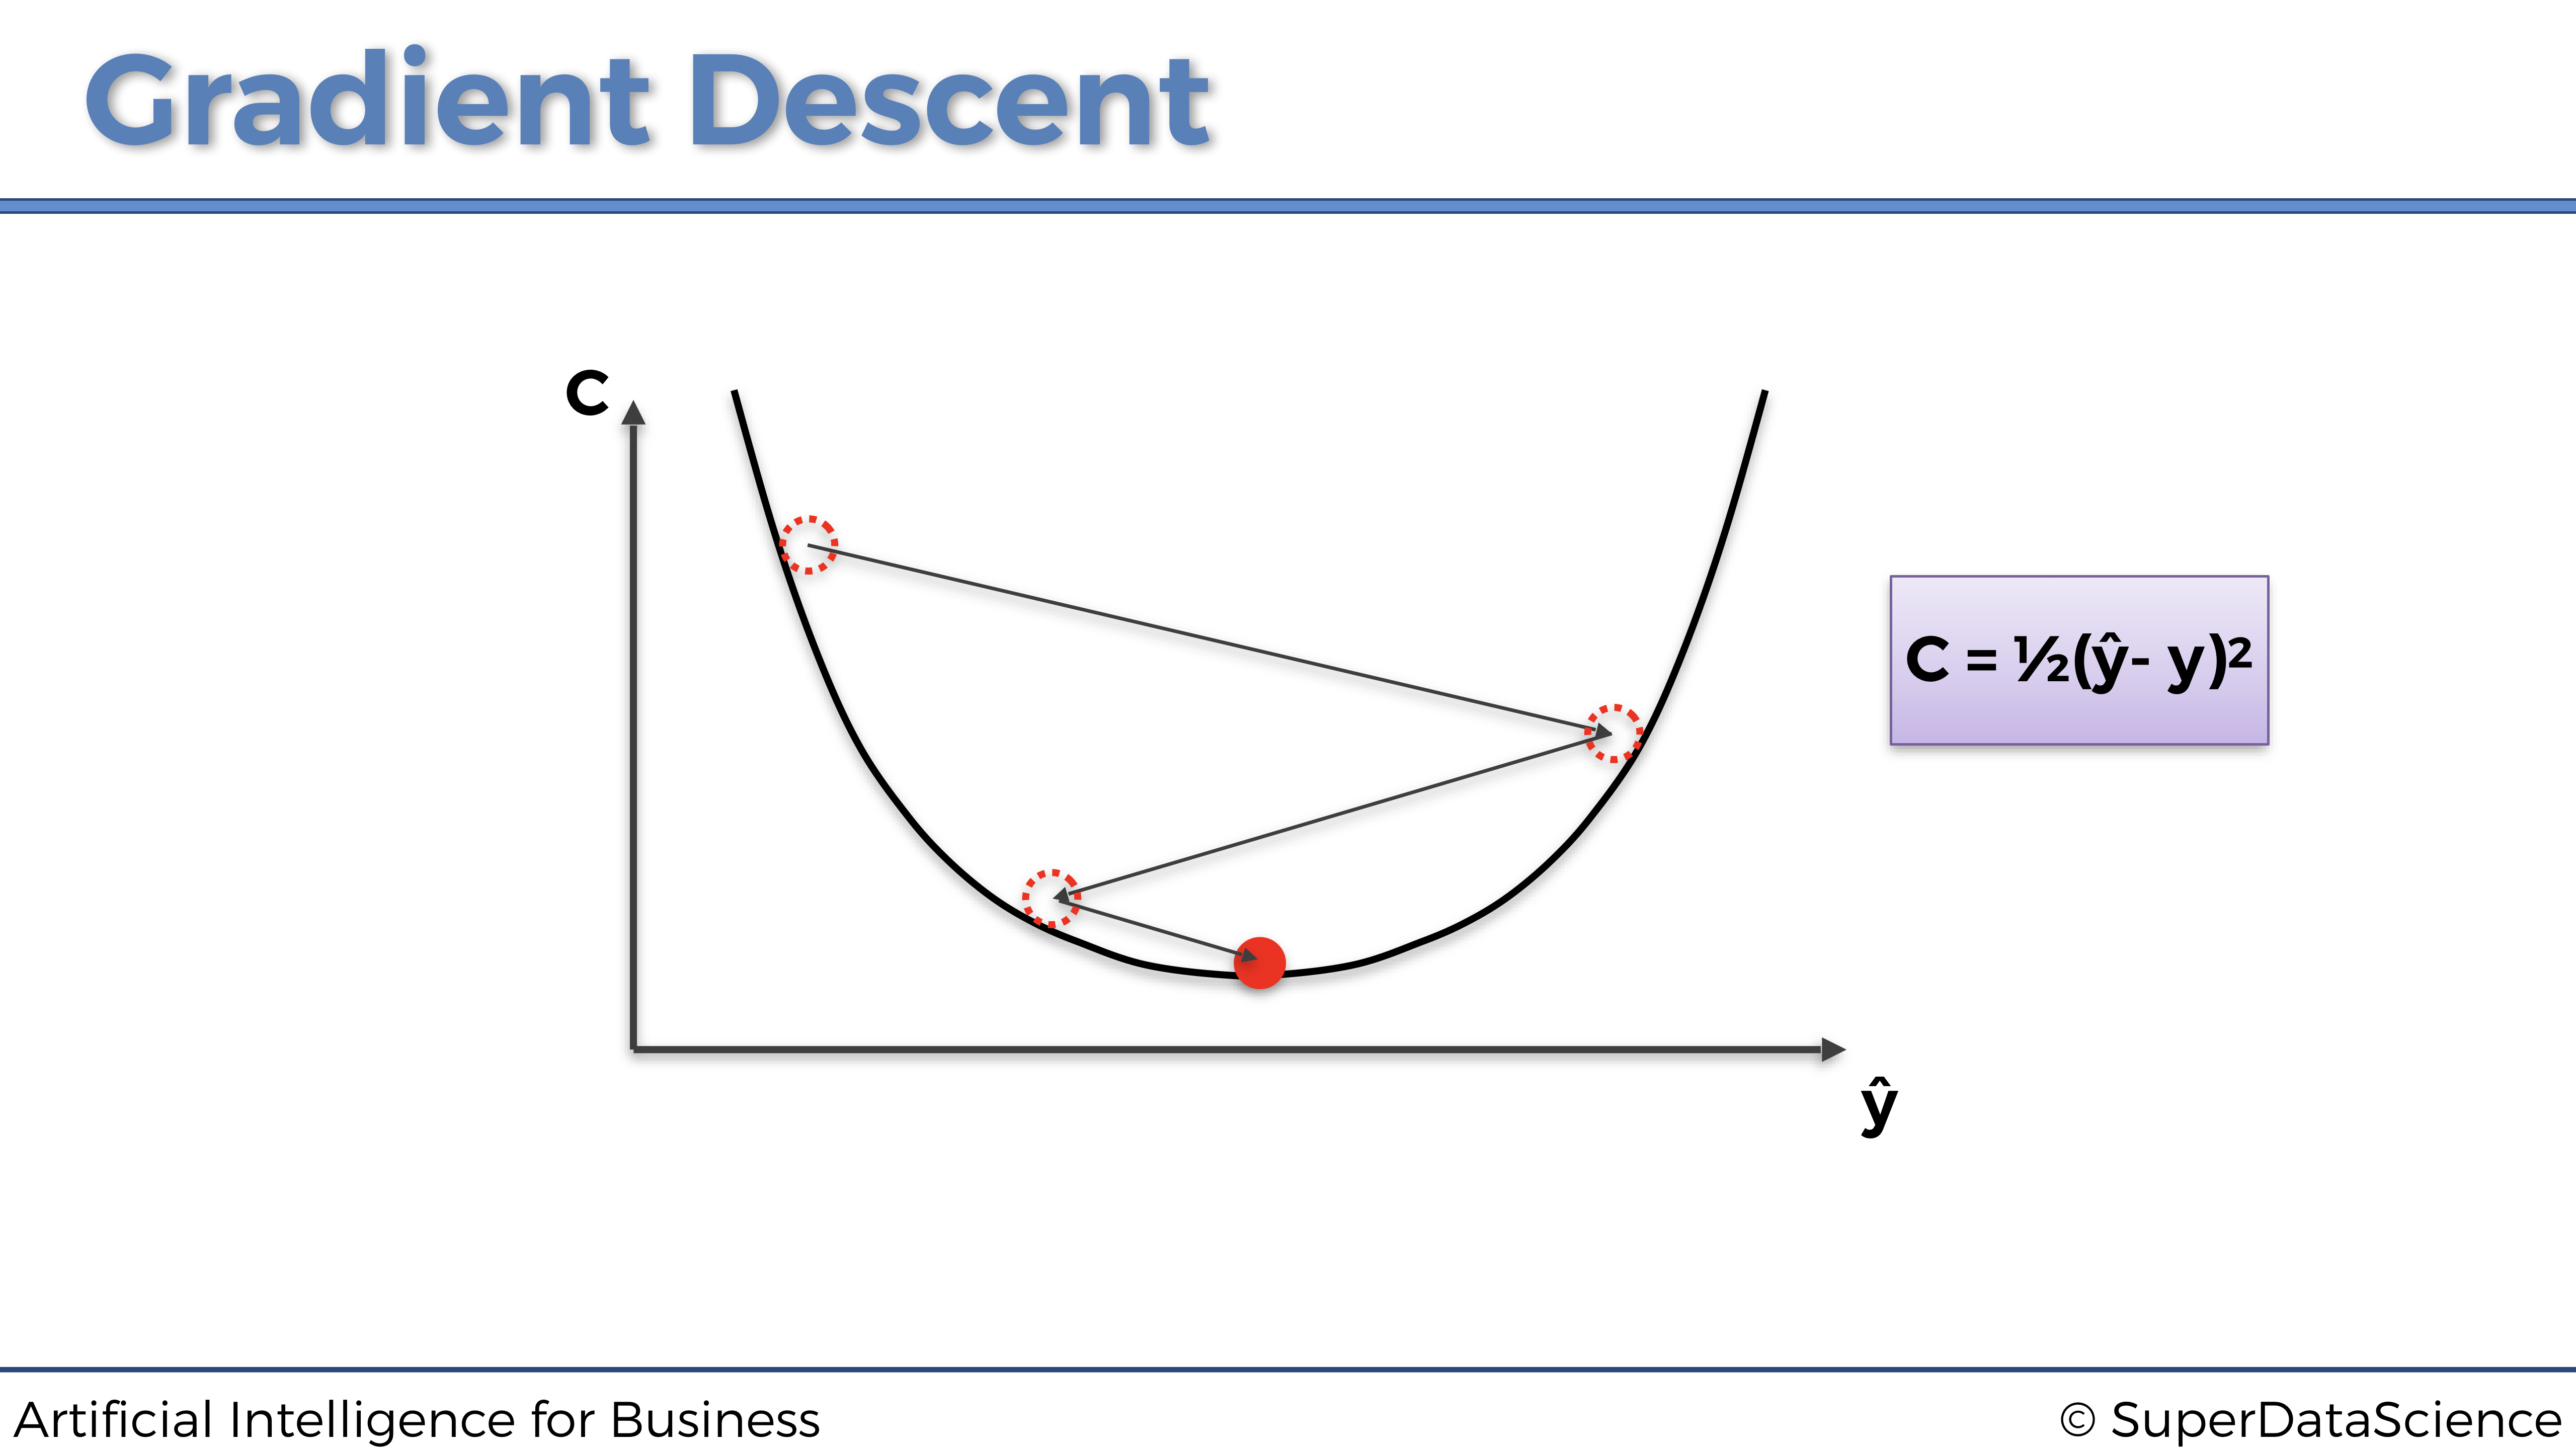
\includegraphics[scale=0.18]{ANN_23.png}
        \end{center}
\end{figure}

And that's it! This is how Gradient Descent operates in one dimension (one parameter). Now you might ask: ``Great, but how does this scale?'' We saw an example of one dimensional optimization, what about two or even 3 dimensions?

Excellent question. Gradient Descent guarantees that this approach scales on as many dimensions as needed, provided the cost function is convex. In fact, if the cost function is convex, Gradient Descent will find the absolute minimum of the cost function. Below is an example in 2 Dimensions:

\begin{figure}[!htbp]
        \begin{center}
            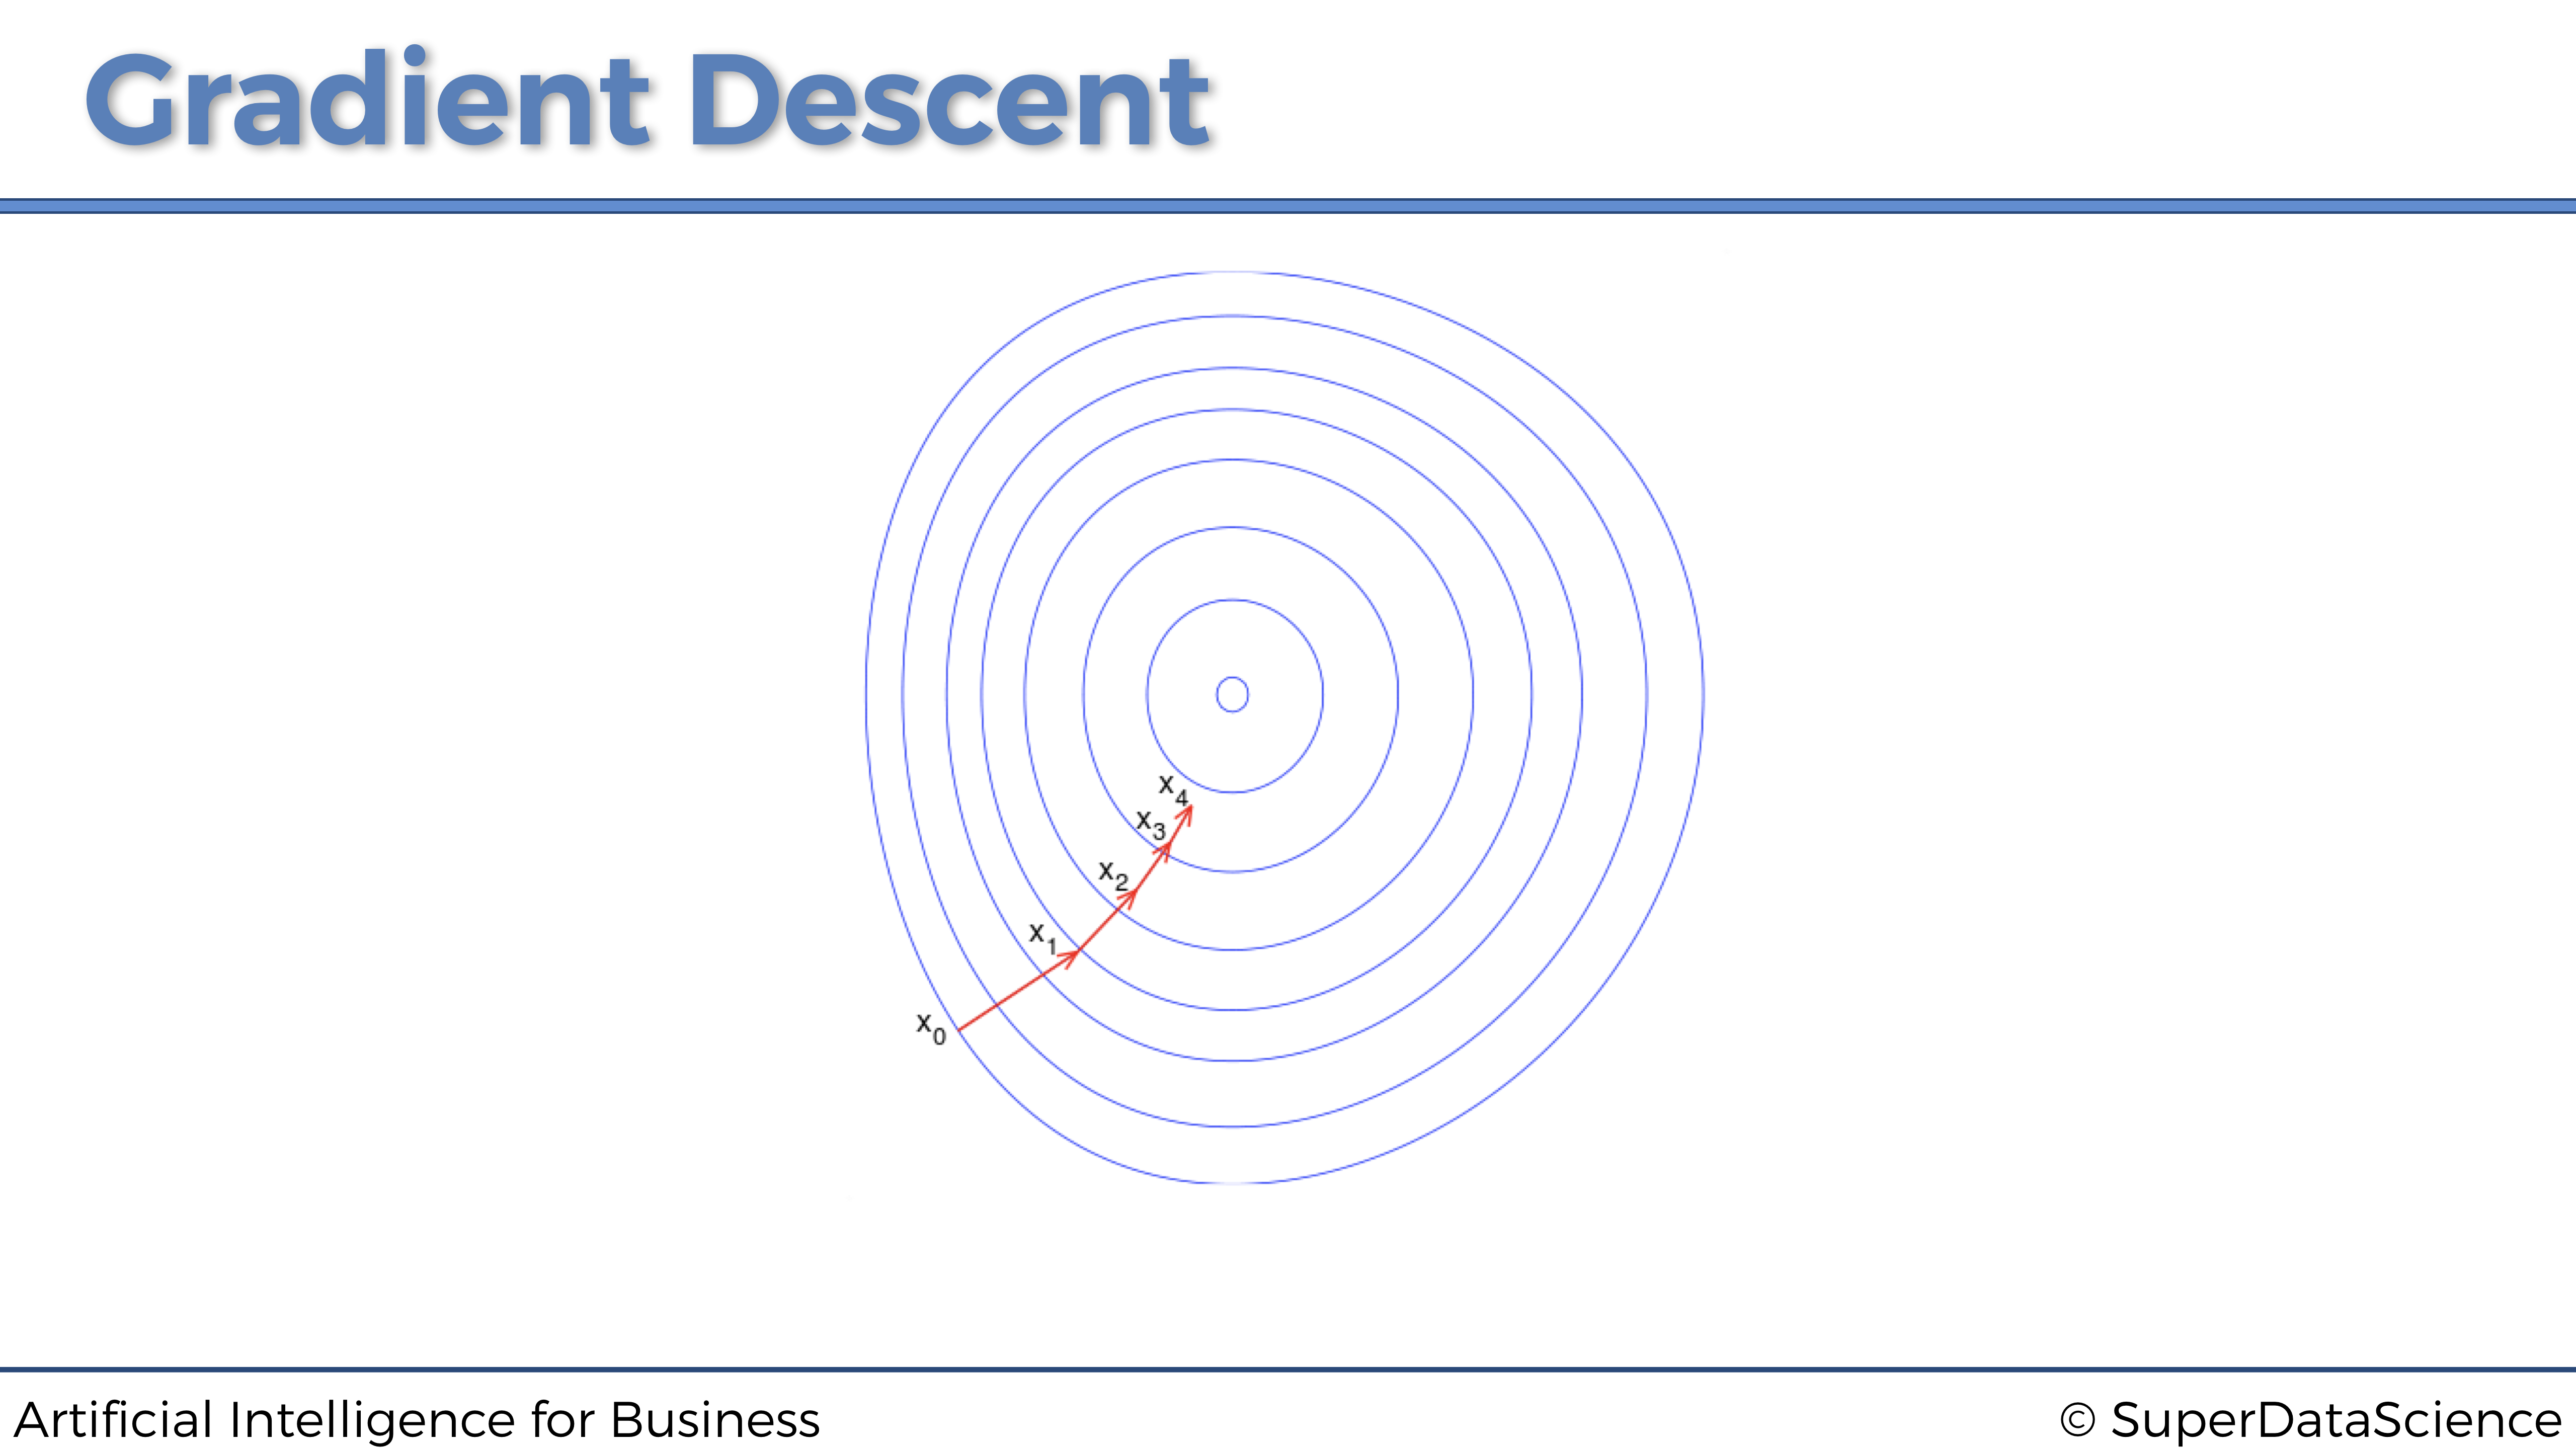
\includegraphics[scale=0.15]{ANN_24.png}
        \end{center}
\end{figure}

However if the cost function is not convex, it will only find a local minimum. Below is an example in 3 Dimensions:

\begin{figure}[!htbp]
        \begin{center}
            \includegraphics[scale=0.15]{ANN_25.png}
        \end{center}
\end{figure}

Now that we understand what Gradient Descent is all about, time to study the most advanced and most effective versions of it:

\begin{enumerate}
    \item Batch Gradient Descent
    \item Mini-Batch Gradient Descent
    \item Stochastic Gradient Descent
\end{enumerate}

\subsection{Batch Gradient Descent}

``Gradient Descent'', ``Batch Gradient Descent'', ``Mini Batch Gradient Descent'', ``Stochastic Gradient Descent''.. There are so many terms and someone who is just starting may found him/her very confused.

The main difference across all of these versions of Gradient Descent is in the way we feed our data to a model, and how often we update our parameters (weights) to move our small red ball. Let's start by explaining Batch Gradient Descent.

Batch Gradient Descent is exactly what we did in Part 2 - Minimizing Costs, where remember we had a batch of inputs feeding the neural network, forward-propagating them to obtain in the end a batch of predictions, which themselves are compared to a batch of targets. The global loss error between the predictions and the targets of the two batches is then computed as the sum of the loss errors between each prediction and its associated target. That global loss is back-propagated into the neural network, where gradient descent or stochastic gradient descent is performed to update all the weights, according to how much they were responsible for that global loss error.

In the next page below is an example of Batch Gradient Descent. The problem to solve is about predicting the score (from 0 to 100 \%) students get at an exam, based on the time spent to study, and the time spent to sleep:

\newpage

\begin{figure}[!htbp]
        \begin{center}
            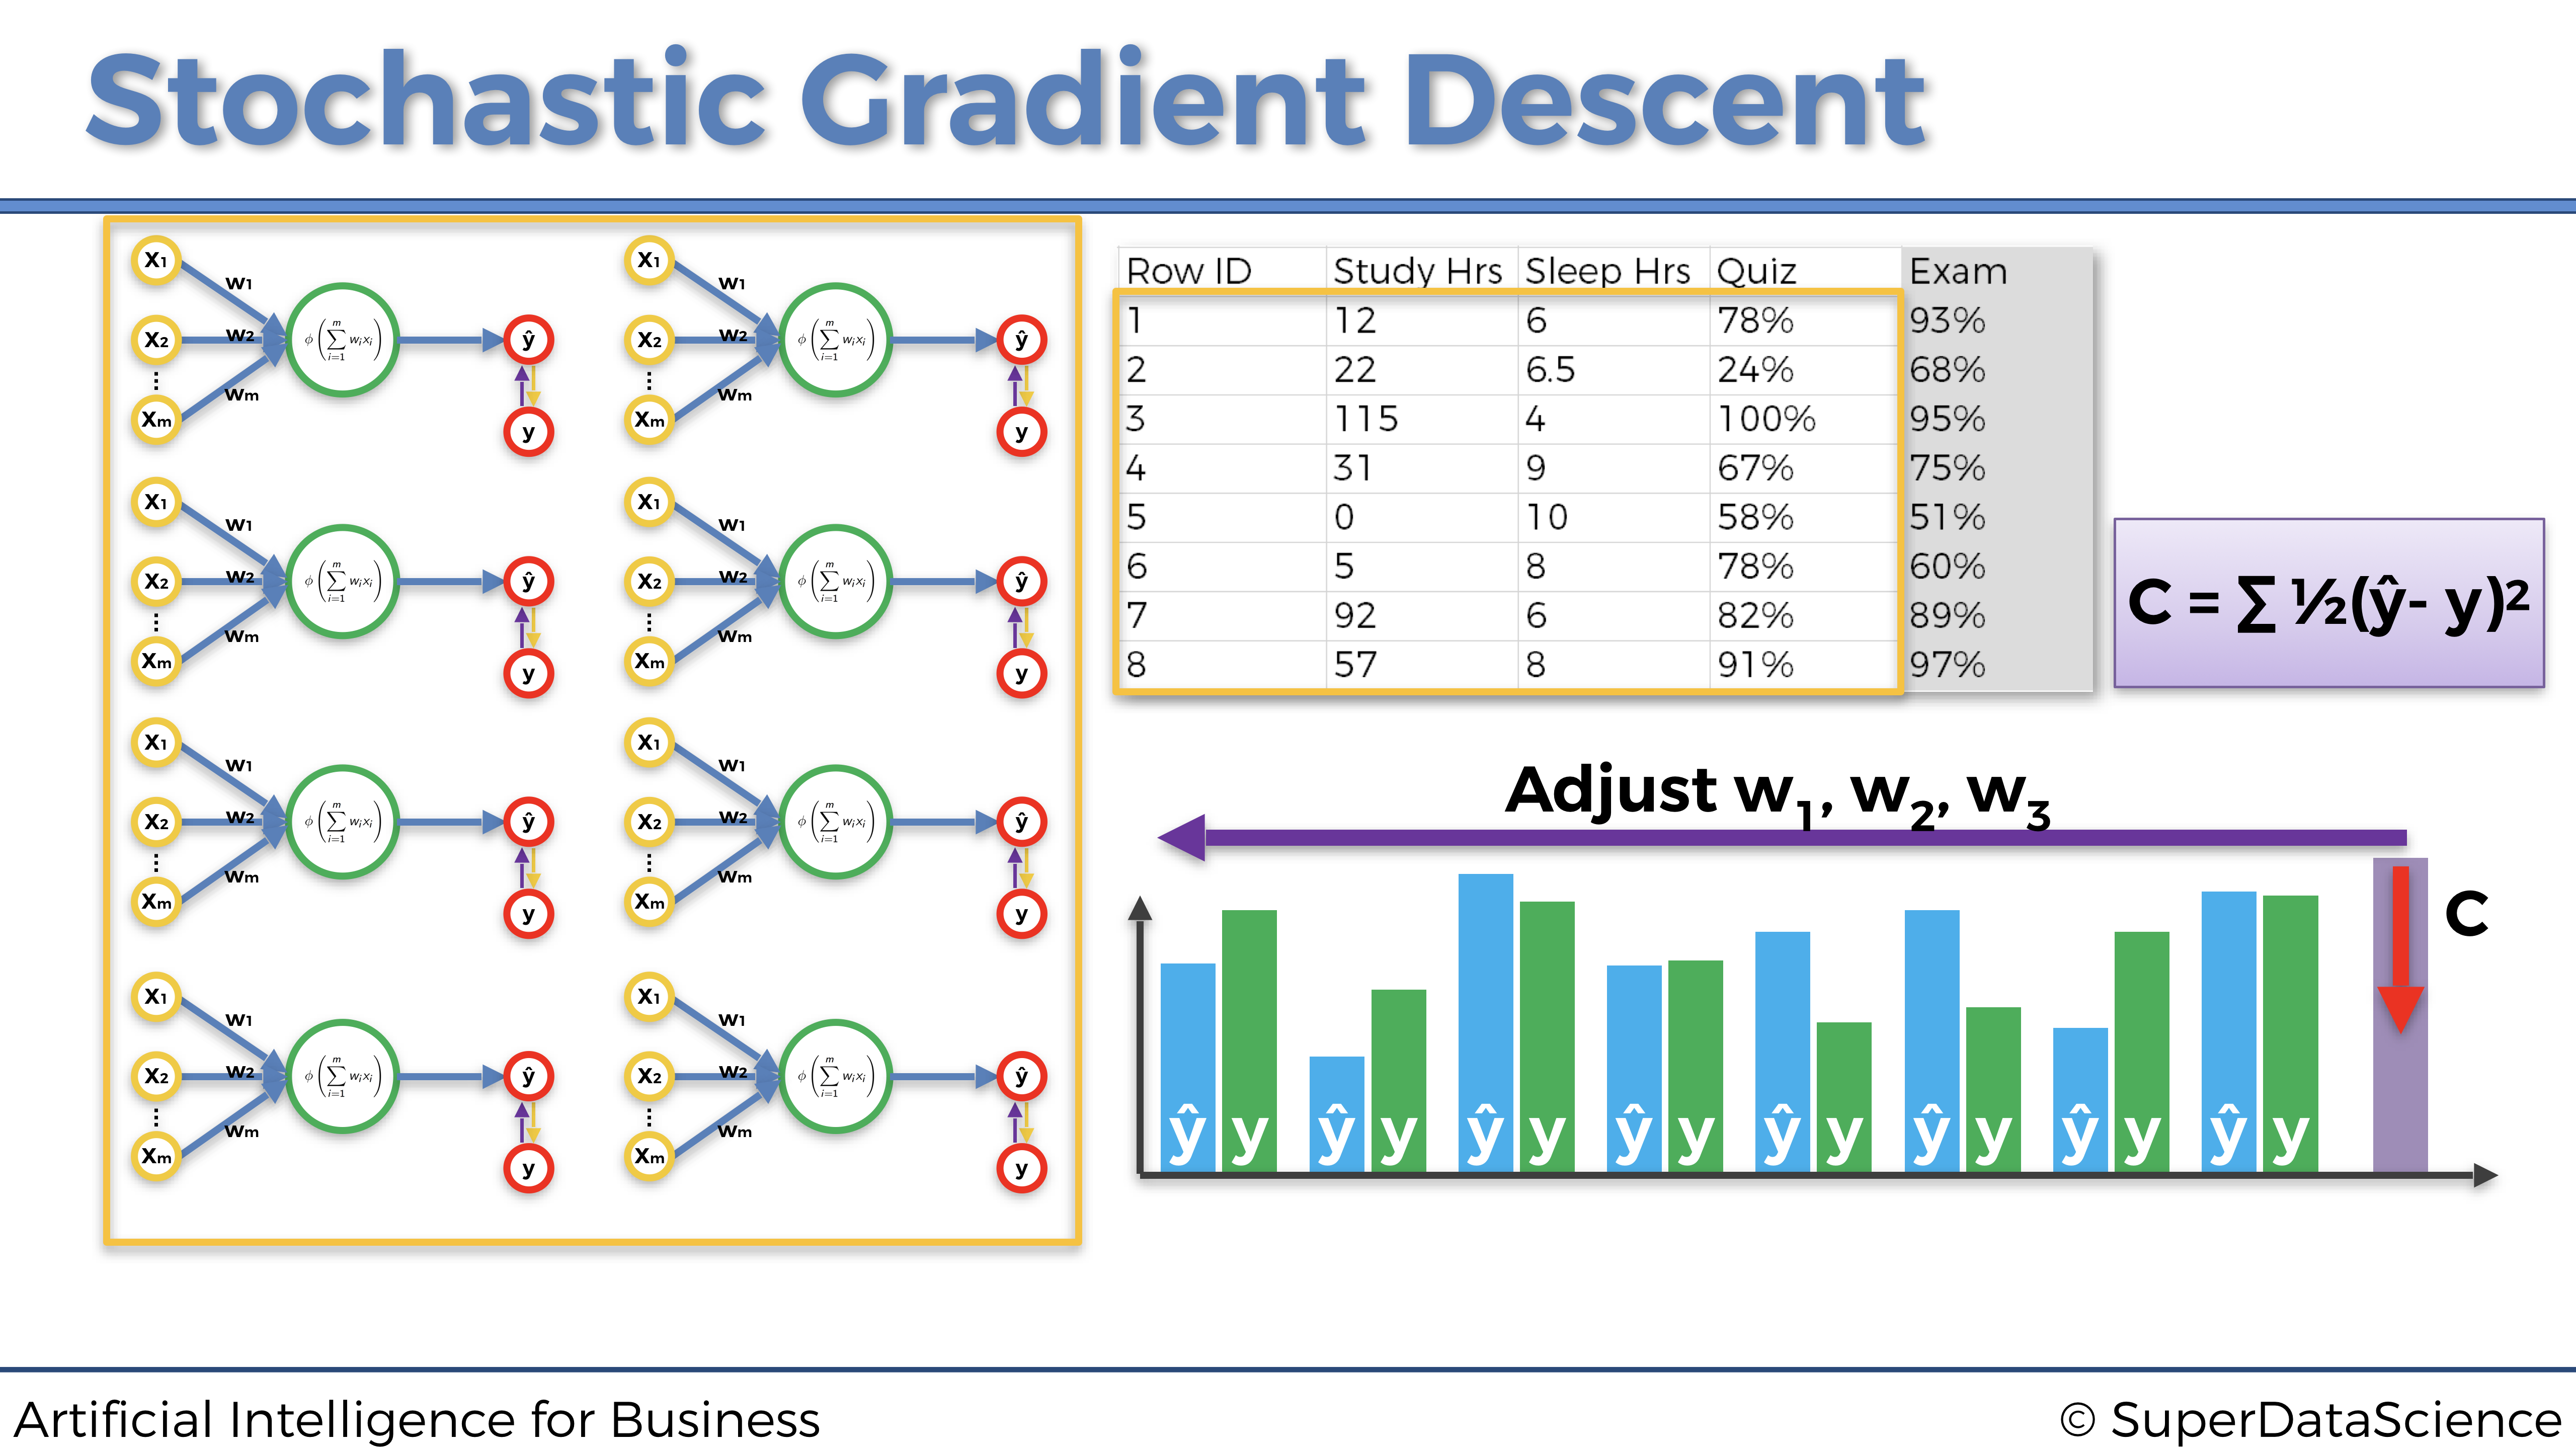
\includegraphics[scale=0.18]{ANN_26.png}
        \end{center}
\end{figure}

An important thing to note on this graphic above is that these are not multiple neural networks, but a single one represented by separate weight updates. And again, as we can notice in this example of Batch Gradient Descent, we feed all of our data to the model at once. This will produce collective updates of the weights and fast optimization of the network. However, there is the bad side of this as well. There is once again the possibility to get stuck at a local minimum, as we can see in the next graphic below:

\begin{figure}[!htbp]
        \begin{center}
            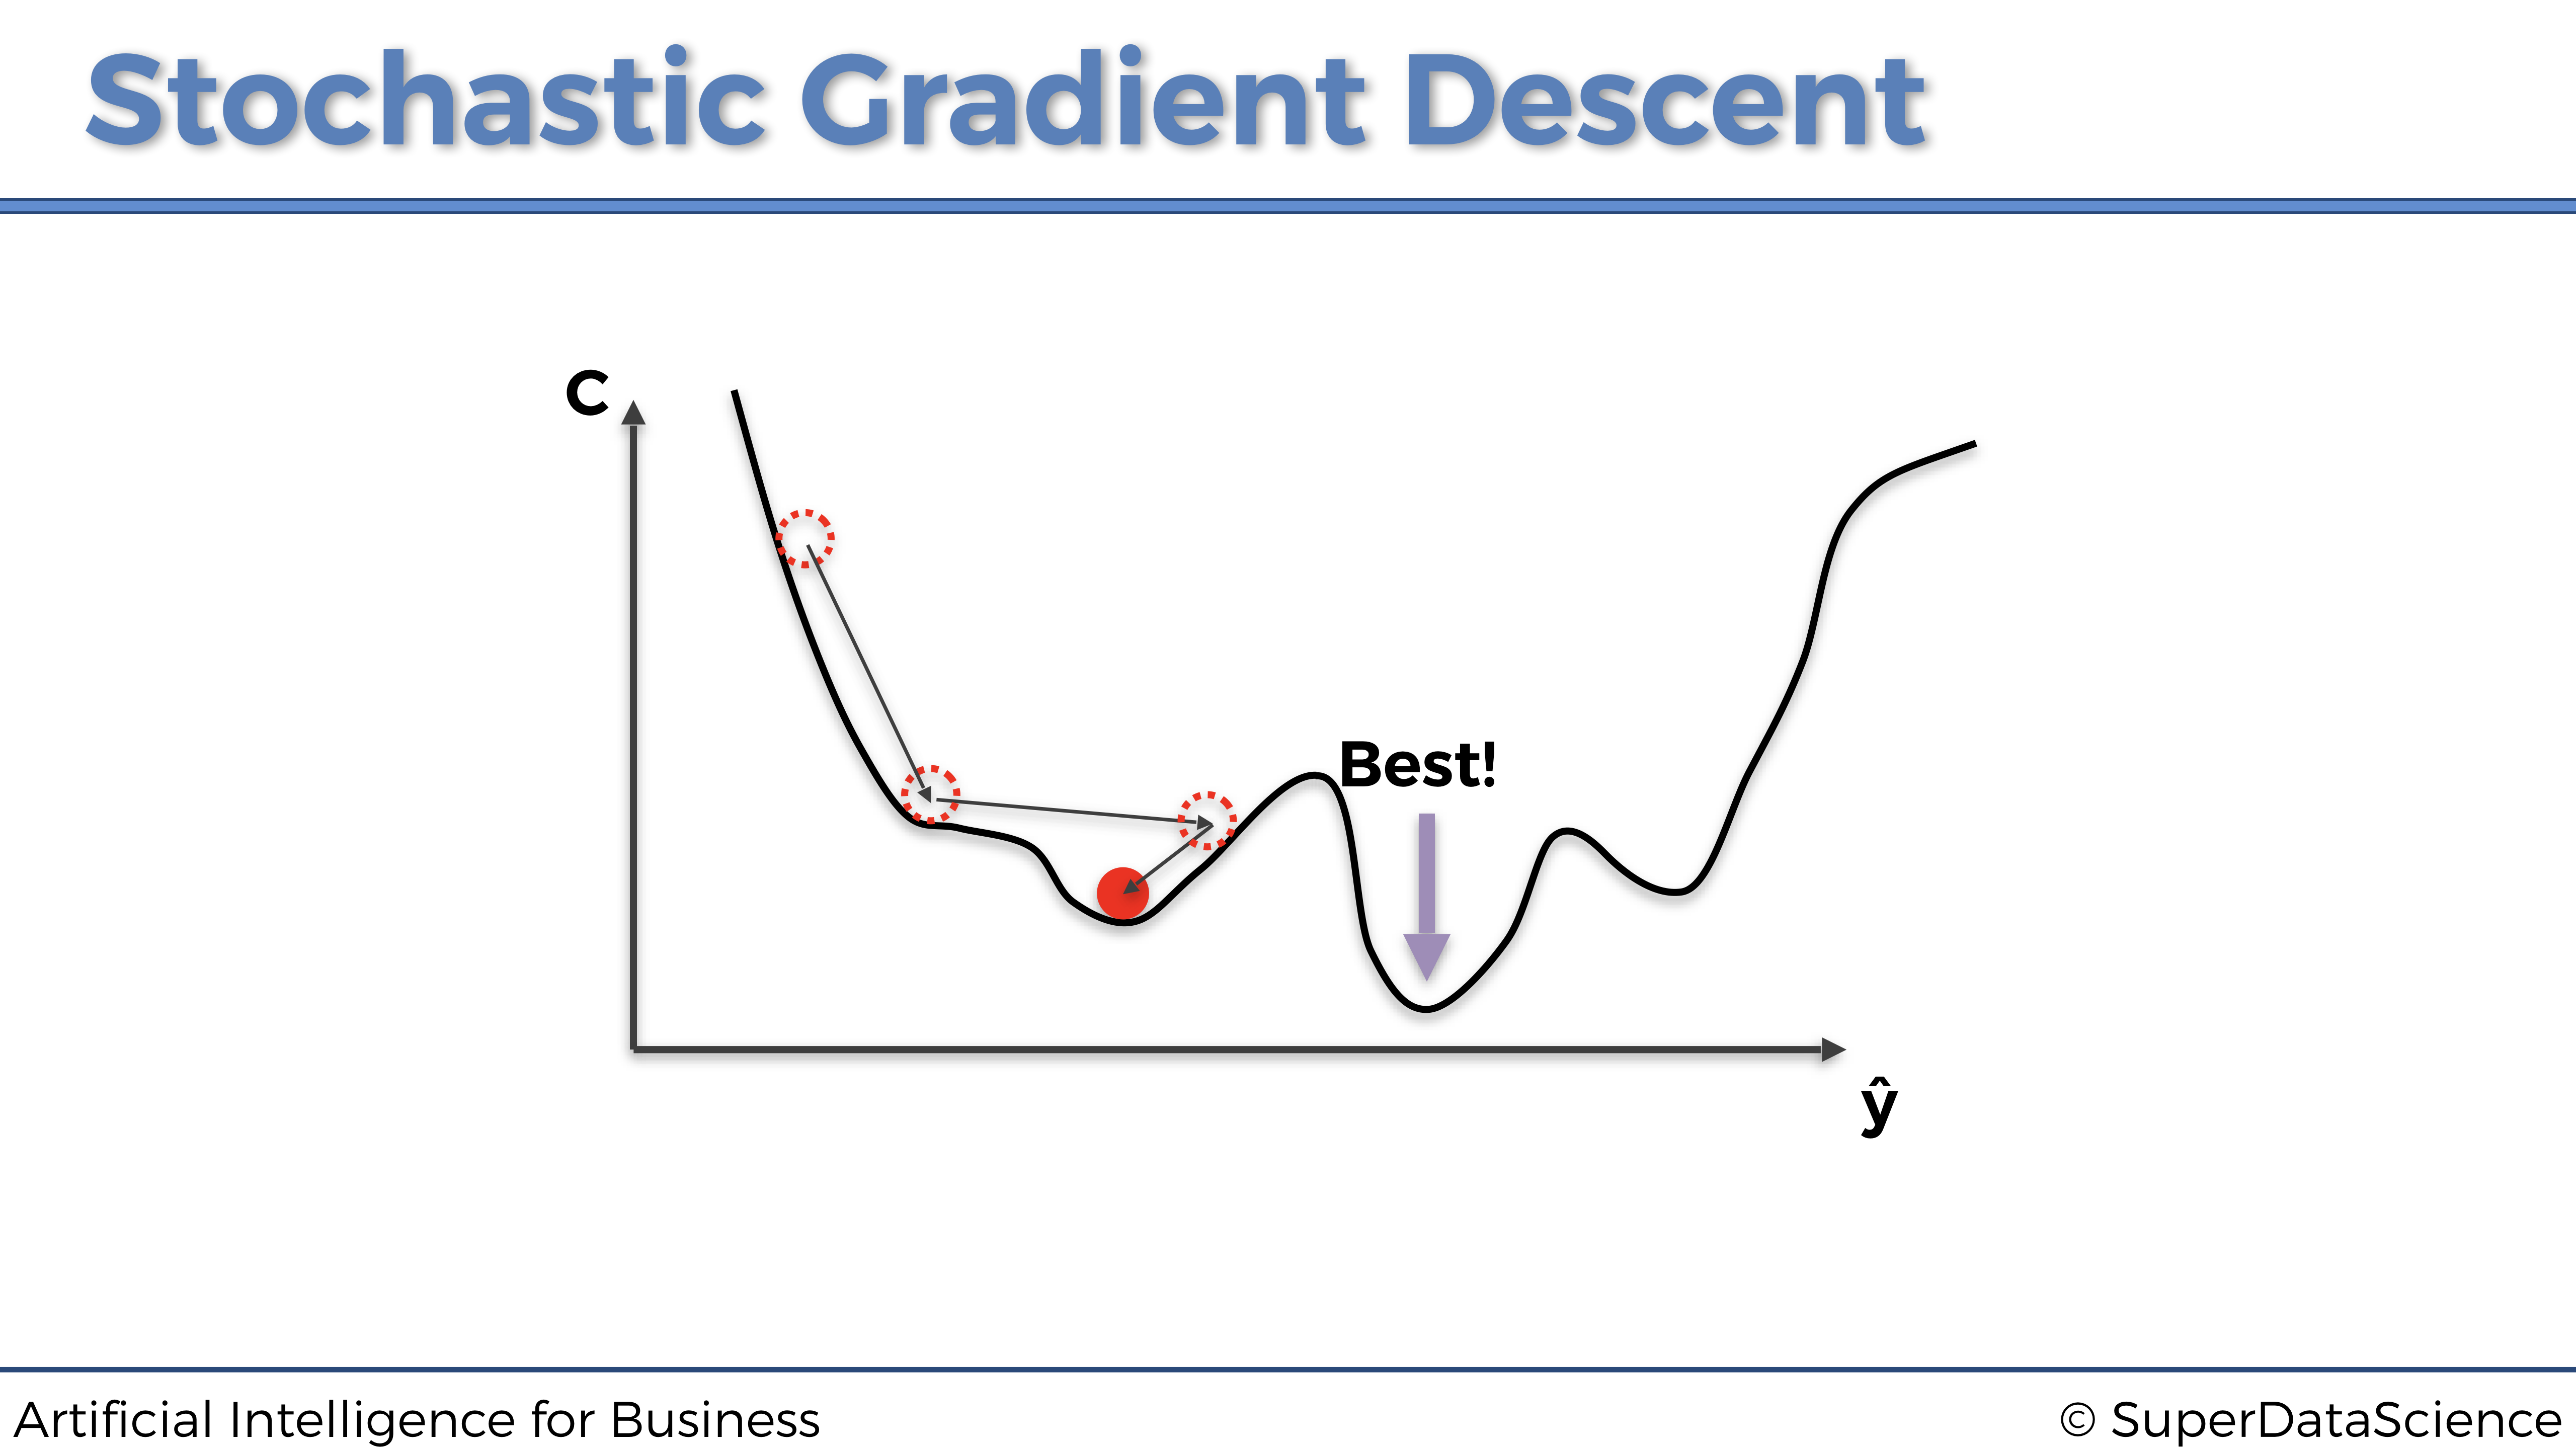
\includegraphics[scale=0.18]{ANN_30.png}
        \end{center}
\end{figure}

\newpage

The reason why this happens was explained a bit earlier: it is because the cost function in the graphic above is not convex. And this type of optimization (simple Gradient Descent) requires the cost function to be convex. If that is not the case we can find ourselves stuck in a local minimum and never find the global minimum having the optimal parameters. On the other hand, below is an example of a convex cost function, the same one as we saw earlier:

\begin{figure}[!htbp]
        \begin{center}
            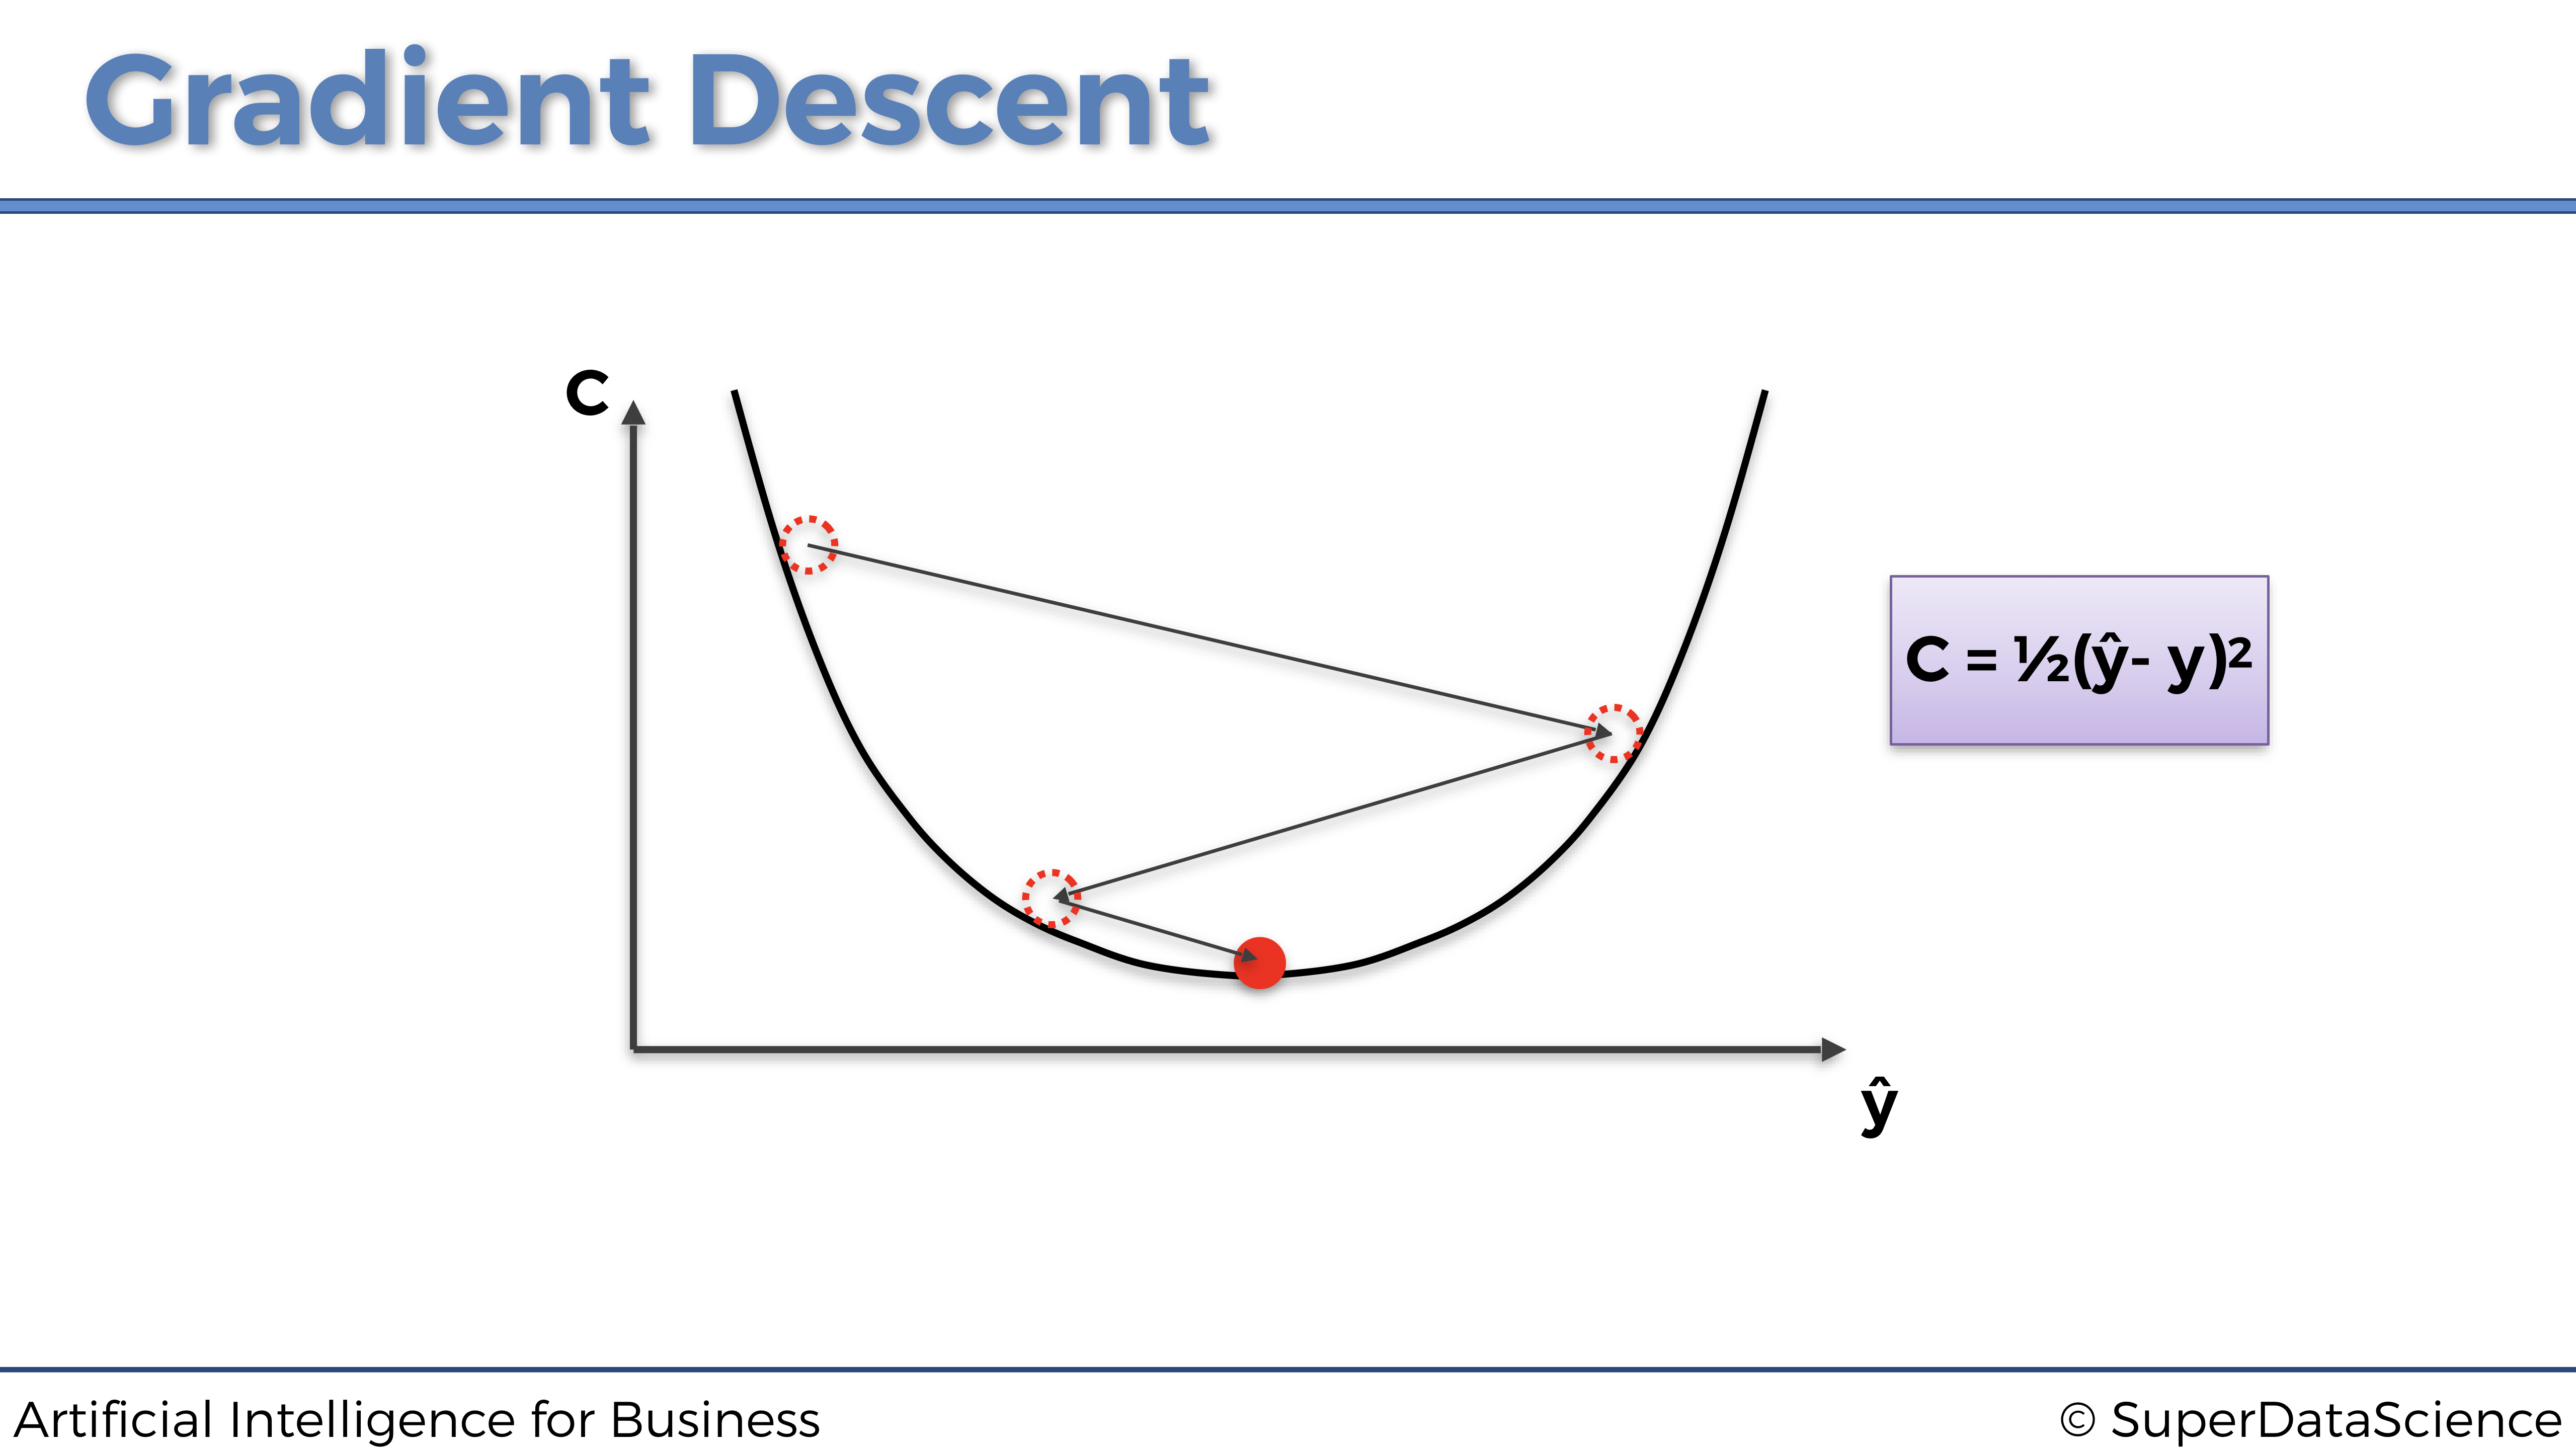
\includegraphics[scale=0.18]{ANN_23.png}
        \end{center}
\end{figure}

In simple terms, a function is convex if it has only one global minimum. And the graph of a convex function has the bowl shape.

However, in most of the problems, including the business problems, the cost function will not be convex (as in this same graphic example in 3D below), thus not allowing simple Gradient Descent to perform well. This is where Stochastic Gradient Descent comes into play.

\begin{figure}[!htbp]
        \begin{center}
            \includegraphics[scale=0.13]{ANN_25.png}
        \end{center}
\end{figure}

\subsection{Stochastic Gradient Descent}

Stochastic Gradient Descent (SGD) comes to save the day. It indeed provides better results overall, preventing the algorithm to get stuck in a local minimum. However, as its name suggests, it is stochastic, or in other words, random. Because of this property, no matter how many times you run the algorithm, the process will always be slightly different. And that, regardless of the initialization.

Stochastic Gradient Descent does not run on the whole dataset at once but instead input by input. Hence, the process goes like this:

\begin{enumerate}
    \item Input a single observation
    \item Get the single prediction
    \item Compute the loss error between the prediction and the target
    \item Back-Propagate the loss error into the neural network
    \item Update the weights with Gradient Descent
    \item Repeat 1. to 5. through the whole dataset
\end{enumerate}

Let's represent the three first iterations on the three first single inputs for this same example given earlier about predicting the scores at an exam:

\textbf{First Input Row of Observation:}

\begin{figure}[!htbp]
        \begin{center}
            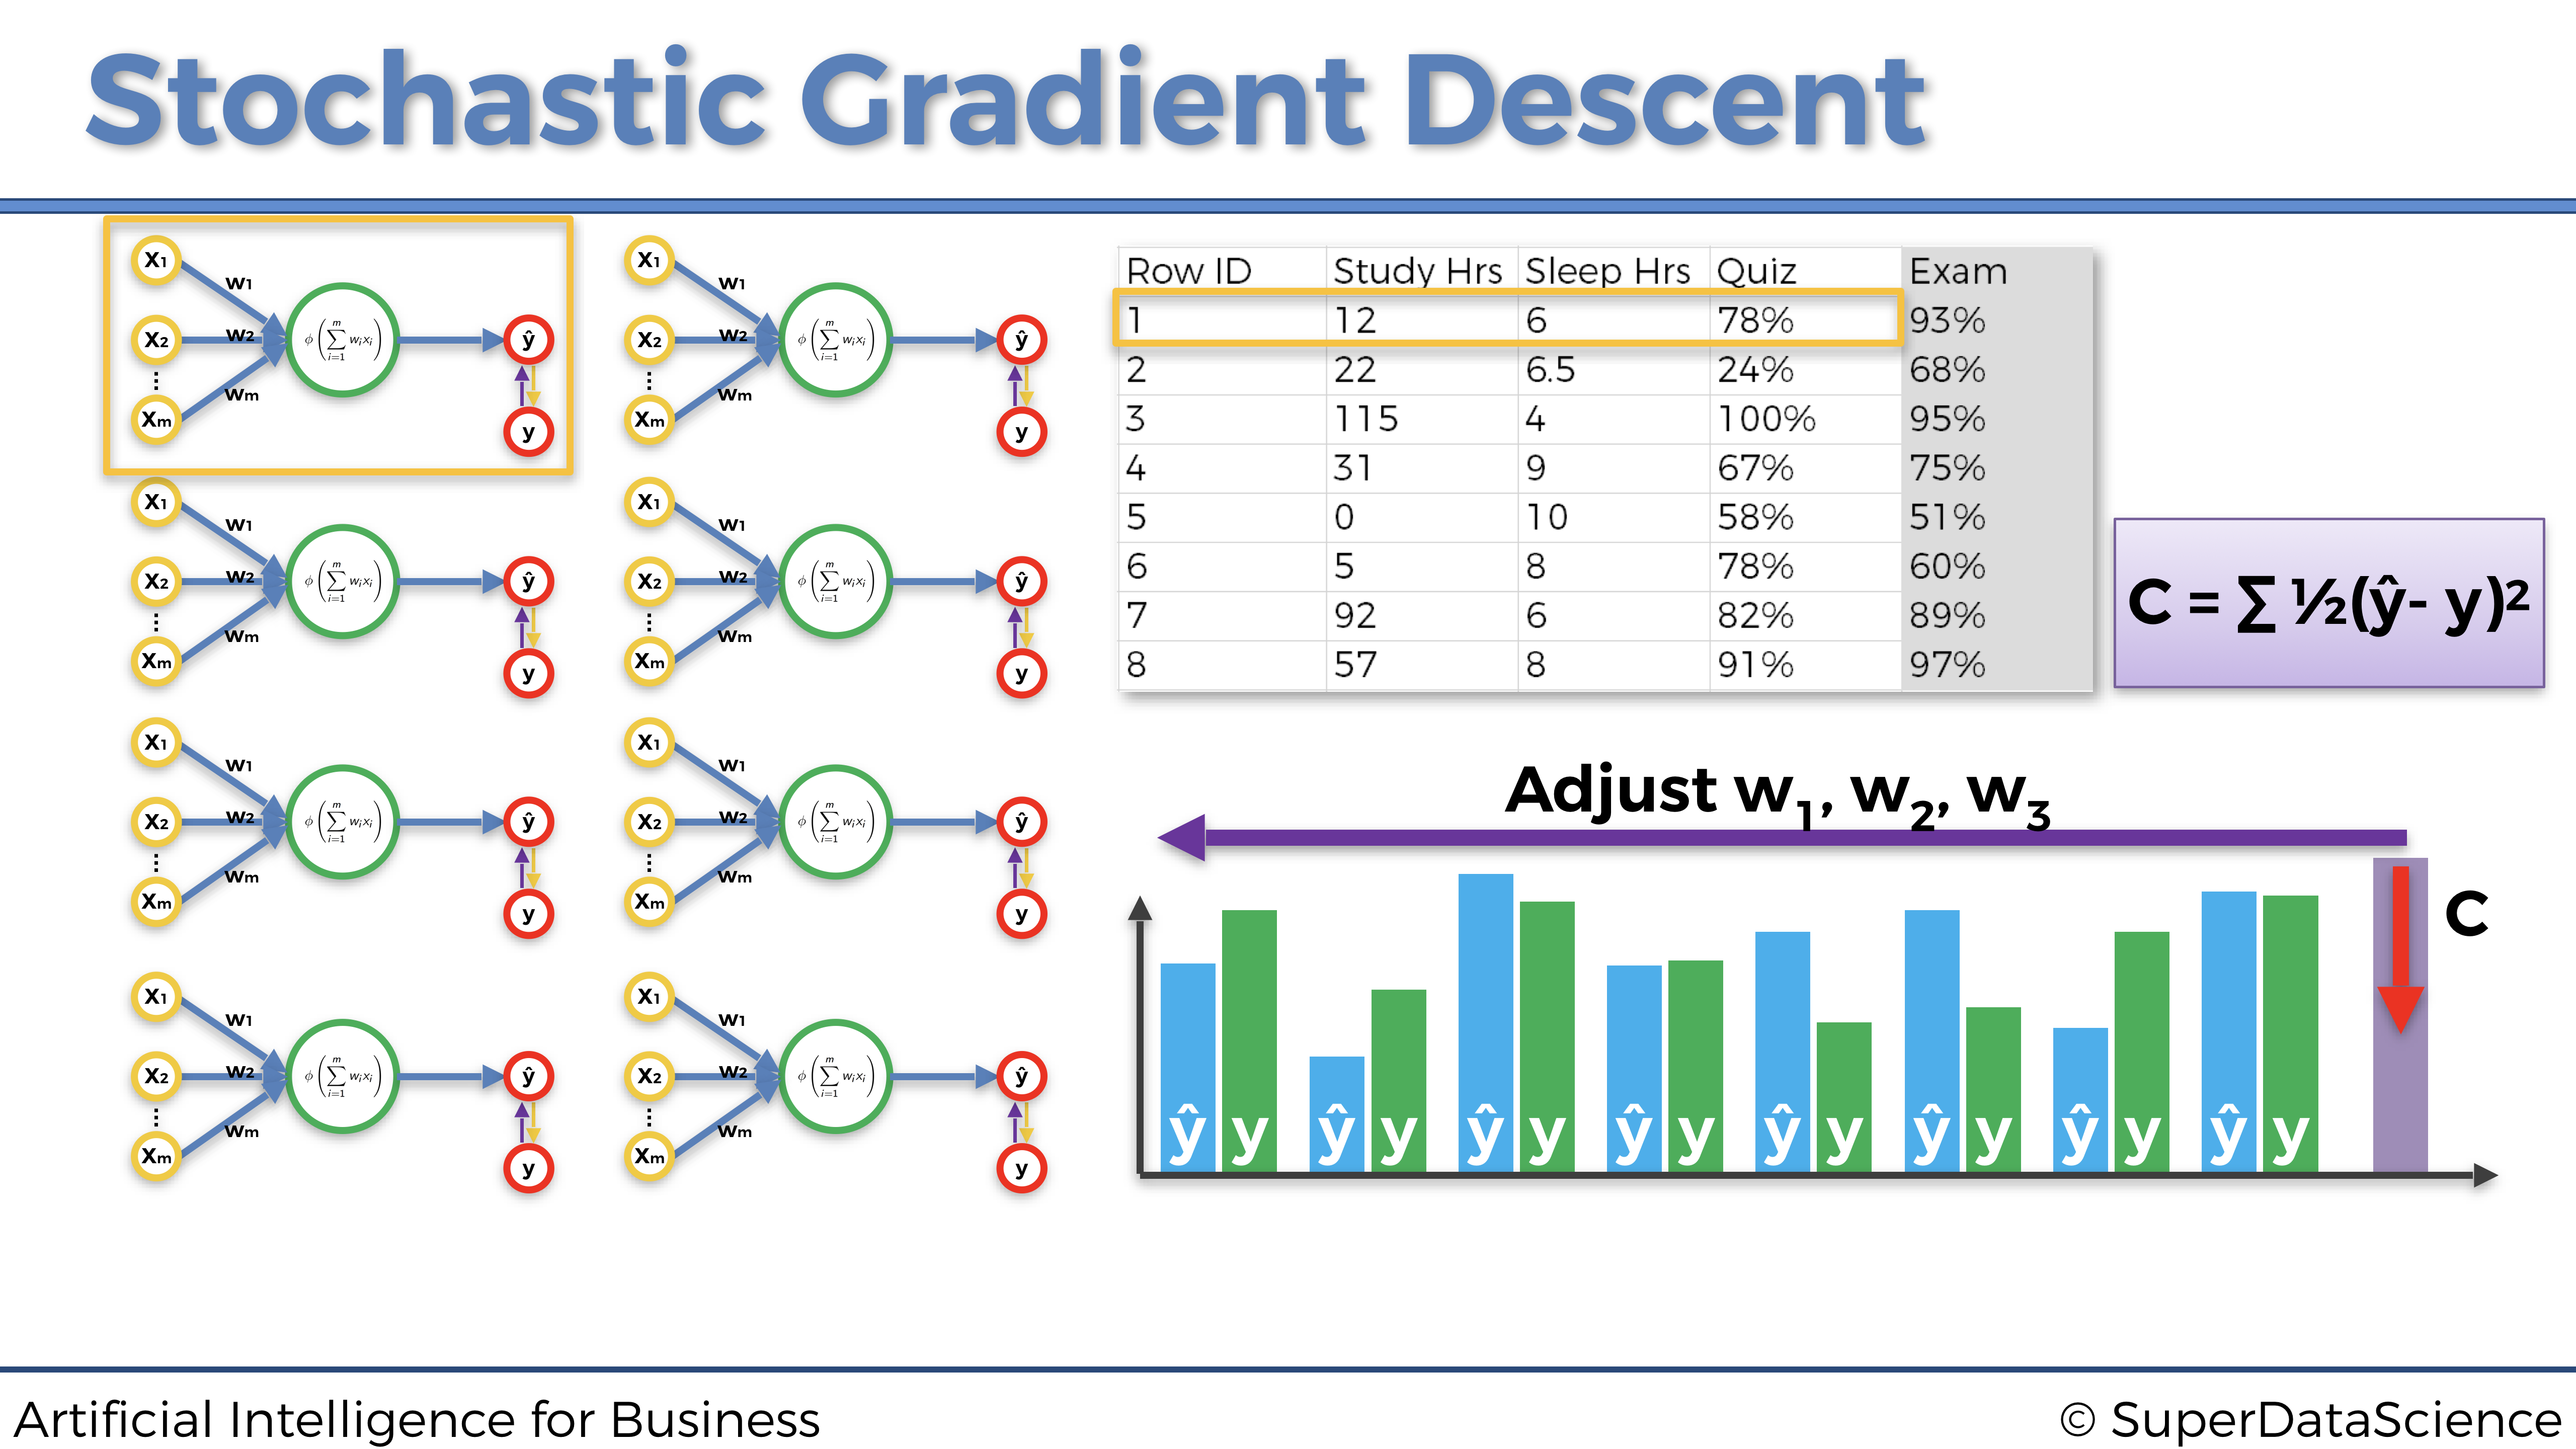
\includegraphics[scale=0.18]{ANN_27.png}
        \end{center}
\end{figure}

\newpage

\textbf{Second Input Row of Observation:}

\begin{figure}[!htbp]
        \begin{center}
            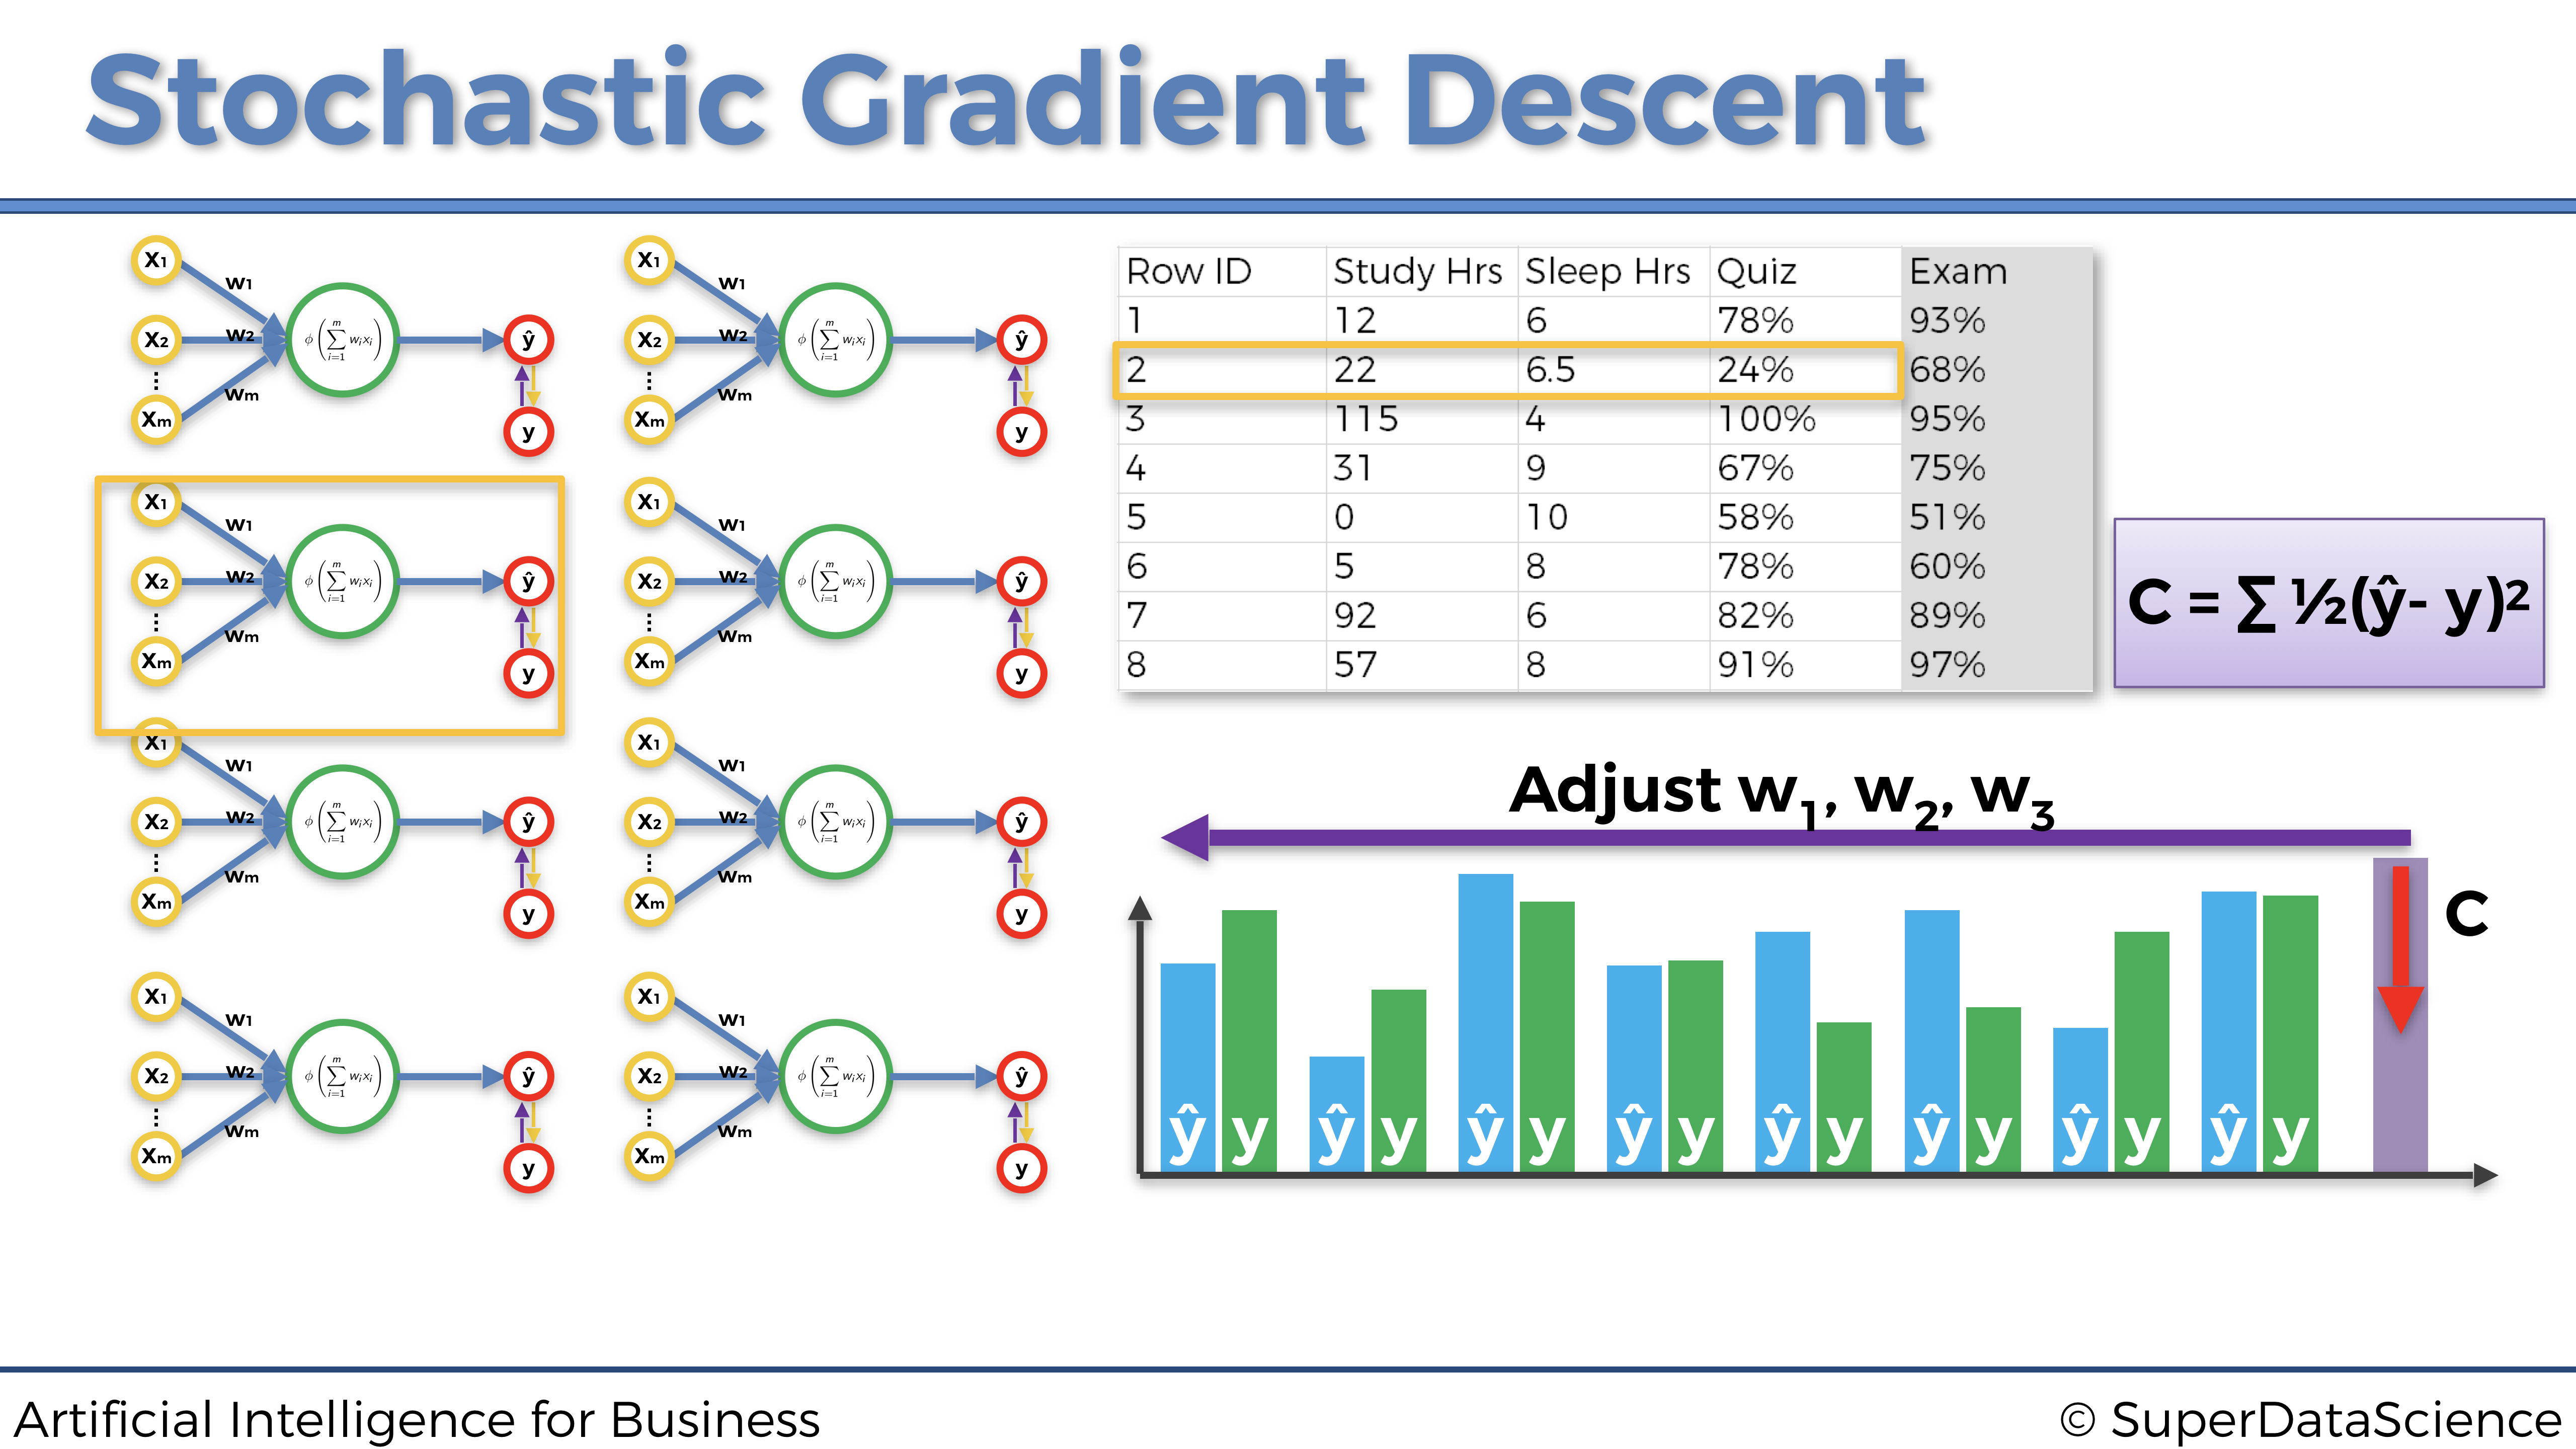
\includegraphics[scale=0.18]{ANN_28.png}
        \end{center}
\end{figure}

\textbf{Third Input Row of Observation:}

\begin{figure}[!htbp]
        \begin{center}
            \includegraphics[scale=0.18]{ANN_29.png}
        \end{center}
\end{figure}

Each of the three graphics above is an example of one weights update ran by Stochastic Gradient Descent. As we can see, each time we only input a single row of observation from our dataset to the neural network, then we update the weights accordingly and proceed to the next input row of observation.

At first glance, Stochastic Gradient Descent seems slower, because we input each row separately. But in reality, it is much faster because of the fact that we don't have to load the whole dataset in the memory, nor to wait for whole dataset to pass through the model updating the weights.

To finish this section, let's recap on the difference between Batch Gradient Descent and Stochastic Gradient Descent, with the following graphic:

\begin{figure}[!htbp]
        \begin{center}
            \includegraphics[scale=0.18]{ANN_31.png}
        \end{center}
\end{figure}

\subsection{Mini-Batch Gradient Descent}

Mini-Batch Gradient Descent is using the best from both worlds to combine Batch Gradient Descent with Stochastic Gradient Descent. This is done by feeding the neural network with batches of data instead of feeding single input rows of observations one by one or the whole dataset at once.

This approach is faster than classical Stochastic Gradient Descent and prevents from getting stuck in the local minimum. This also helps when people don't have enough computing resources to load the whole dataset in the memory, or enough processing power to get full benefit of Stochastic Gradient Descent.

\subsection{Optimizers}

The optimizer is exactly the tool that will update the weights of the Neural Network through Stochastic Gradient Descent. Up to this point we have only mentioned the Adam optimizer (see Part 2 - Minimizing Costs), which is the most common optimizer used for the Deep Learning and Deep Reinforcement Learning models. Nevertheless there are a lot more optimizers which have their own benefits and applications.

Let's go through the most famous and widely used Gradient Descent optimizers.

\newpage

\subsubsection{Momentum Optimizer}

The classical Stochastic Gradient Descent has very big oscillations, which leaves room for improvement. The Momentum optimizer handles these big oscillations by adding fractions of the directions calculated in the previous step to the current step. This amplifies the speed of the current direction update. In the graphic just below we can see and compare the Classical SGD and the Momentum SGD in action:

\begin{figure}[!htbp]
        \begin{center}
            \includegraphics[scale=0.75]{ANN_32.png}
        \end{center}
\end{figure}

The benefits of the Momentum Optimizer are the following:

\begin{itemize}
    \item Faster Convergence
    \item Less Oscillations
\end{itemize}

But the Momentum Optimizer also has drawbacks, which are the following:

\begin{itemize}
    \item Tendency to overshoot the global minimum of the cost function because of the momentum.
    \item Less frequent in Deep Learning libraries, which thus requires the know-how of its implementation.
\end{itemize}

\newpage

\subsubsection{The Nesterov Accelerated Gradient Optimizer}

Yuri Nesterov solved the momentum the overshot minimum problem by reversing the calculation order in the update formula:

\begin{figure}[!htbp]
        \begin{center}
            \includegraphics[scale=0.6]{ANN_33.png}
        \end{center}
\end{figure}

\subsubsection{The AdaGrad (Adaptive Gradients) Optimizer}

The idea of adapting our updates according to the slope of the error function, coming from the Nesterov optimizer, is taken and applied in the AdaGrad Optimizer while optimizing the learning rate as well.

Hence, in the AdaGrad optimizer we have the same principle, not only applied on gradients but also on the learning rate.

Here are the benefits of this optimizer:

\begin{itemize}
    \item The AdaGrad optimizer allows to make big updates for infrequent parameters.
    \item And it allows to make small updates for frequent parameters.
\end{itemize}

And here are the drawbacks:

\begin{itemize}
    \item The Learning Rate is always decreasing, this could lead to very small, if any updates.
    \item Less frequent in Deep Learning libraries, which thus requires the know-how of its implementation.
\end{itemize}

\subsubsection{The AdaDelta Optimizer}

The AdaDelta Optimizer was invented to fix that decreasing learning rate issue of the AdaGrad Optimizer (first drawback). No need to get in further details, we just needed to introduce the AdaDelta optimizer and its particularity in order to understand the strength of the most widely used and most effective optimizer: the Adam Optimizer.

\subsubsection{The Adam (Adaptive Moment Estimation) Optimizer}

The Adam Optimizer is an improvement over the AdaDelta Optimizer. The idea behind it is to store in a memory the momentum changes, as we calculate the learning rate for each parameter separately.

Now remember the benefits of the Adam Optimizer, which are to be considered whenever building a Neural Network.

\begin{itemize}
    \item It is one of the most powerful optimizers.
    \item It is always pre-implemented in the Deep Learning libraries (Keras, TensorFlow, PyTorch). You will not miss it.
\end{itemize}

Of course, this is the one we use when building the Artificial Brain of our AI in Part 2 - Minimizing the Costs. Let's again provide the code that builds this artificial brain and notice, at the last line of code, the simplicity of selecting the Adam Optimizer:

\begin{lstlisting}
# Artificial Intelligence for Business - Case Study 2
# Building the Brain

# Importing the libraries
from keras.layers import Input, Dense
from keras.models import Model
from keras.optimizers import Adam

# BUILDING THE BRAIN

class Brain(object):
    
    # BUILDING A FULLY CONNECTED NEURAL NETWORK DIRECTLY INSIDE THE INIT METHOD
    
    def __init__(self, learning_rate = 0.001, number_actions = 5):
        self.learning_rate = learning_rate
        
        # BUILDIND THE INPUT LAYER COMPOSED OF THE INPUT STATE
        states = Input(shape = (3,))
        
        # BUILDING THE FULLY CONNECTED HIDDEN LAYERS
        x = Dense(units = 64, activation = 'sigmoid')(states)
        y = Dense(units = 32, activation = 'sigmoid')(x)
        
        # BUILDING THE OUTPUT LAYER, FULLY CONNECTED TO THE LAST HIDDEN LAYER
        q_values = Dense(units = number_actions, activation = 'softmax')(y)
        
        # ASSEMBLING THE FULL ARCHITECTURE INSIDE A MODEL OBJECT
        self.model = Model(inputs = states, outputs = q_values)
        
        # COMPILING THE MODEL WITH AN MSE LOSS FUNCTION AND THE ADAM OPTIMIZER
        self.model.compile(loss = 'mse', optimizer = Adam(lr = learning_rate))
\end{lstlisting}

\newpage

\section{Annex 2: Three Extra AI Models}

As a Bonus, in this section we provide three extra AI models, closer to the State of the Art. However, these AI models are not necessarily adapted to solve business problems, but more to solve specific tasks like playing games or training a virtual robot to walk. We are going to study three powerful models, including two in the Deep Reinforcement Learning branch of AI, and one in the Policy Gradient branch:

\begin{enumerate}
    \item Deep Convolutional Q-Learning (Deep RL)
    \item A3C (Deep RL)
    \item Augmented Random Search (Policy Gradient)
\end{enumerate}

\subsection{Deep Convolutional Q-Learning}

In the previous section, our inputs were vectors encoded values defining the states of the environment. But since an encoded vector doesn't preserve the spatial structure of an image, this is not the best form to describe a state. The spatial structure is indeed important because it gives us more information to predict the next state, and predicting the next state is of course essential for our AI to know what is the right next move. Therefore we need to preserve the spatial structure and to do that, our inputs must be 3D images (2D for the array of pixels plus one additional dimension for the colors). In that case, the inputs are simply the images of the screen itself, exactly like what a human sees when playing the game. Following this analogy, the AI acts like a human: it observes the input images of the screen when playing the game, the input images go into a convolutional neural network (the brain for a human) which will detect the state in each image. However, this convolutional neural network doesn't contain pooling layers, because they would loose the location of the objects inside the image, and of course the AI need to keep track of the objects. Therefore we only keep the convolutional layers, and then by flattening them into a 1-dimensional vector, we get the input of our previous Deep Q-Learning network. Then the same process is being ran.

Therefore in summary, Deep Convolutional Q-Learning is the same as Deep Q-Learning, with the only difference that the inputs are now images, and a Convolutional Neural Network is added at the beginning of the fully-connected Deep Q-Learning network to detect the states (or simply the objects) of the images.

\begin{figure}[!htbp]
        \begin{center}
            \includegraphics[scale=0.3]{DCQL}
            \caption{Deep Convolutional Q-Learning}
        \end{center}
\end{figure}

\newpage

\subsection{Asynchronous Actor-Critic Agents (A3C)}

\subsubsection{A3C Intuition}

So far, the action played at each time has been the output of one neural network, as if only one agent was deciding the strategy to play the game. This will no longer be the case with A3C. This time, we are going to have several agents, each one interacting with its own copy of the environment. Let's say there are \(n\) agents \(A_1\), \(A_2\),\ldots{}, \(A_n\).

Each agent is sharing two networks: the actor and the critic. The critic evaluates the present states, while the actor evaluates the possible values in the present state. The actor is used to make decisions. At each epoch time of training for on agent, it takes the last version of the shared networks and uses the actor during n steps in order to make a decision. Over the n steps, it collects all the observed new states, the values of these new states, the rewards, etc\ldots{} After the n steps, the agent uses the collected observations in order to update the shared models. The times of epoch, and therefore the times of updates of the shared network by the agent are not synchronous, hence the name.

That way, if an unlucky agent starts to be stuck into a suboptimal but attractive policy, it will reach out that state -- because other agents also updated the shared policy before the agent got stuck -- and will continue effective exploration.

In order to explain the update rules of the actor and the critic, let us see the networks as functions that depend on vectors of parameters \(\theta\) (for the actor) and \(\theta_v\) (for the critic).

\subsubsection{The whole A3C Process}

The official A3C algorithm is the one of the Google DeepMind paper, ``Asynchronous Methods for Deep Reinforcement Learning'' (\url{https://arxiv.org/pdf/1602.01783.pdf}). In this paper you will find it in the following S3 algorithm:

\begin{figure}[!htbp]
        \begin{center}
            \includegraphics[scale=0.4]{S3}
            \caption{A3C algorithm (https://arxiv.org/pdf/1602.01783.pdf)}
        \end{center}
\end{figure}

\begin{figure}[!htbp]
        \begin{center}
            \includegraphics[scale=0.4]{A3C}
            \caption{A3C}
        \end{center}
\end{figure}

In this figure above we can clearly see the three As of the A3C:

\begin{itemize}

\item[$\bullet$] \textbf{Asynchronous}: There are several agents, each one having their own copy of the environment, and all asynchronised (playing the game at different times).

\item[$\bullet$] \textbf{Advantage}: The advantage is the difference between the prediction of the actor, $Q(s,a)$, and the prediction of the critic, $V(s)$:

\begin{equation*}
A = Q(s,a) - V(s)
\end{equation*}

\item[$\bullet$] \textbf{Actor-Critic}: Of course we can see the actor and the critic, that therefore generate two different losses: the policy loss and the value loss. The policy loss is the loss related to the predictions of the actor. The value loss is the loss related to the predictions of the critic. Over many epochs of the training, these two losses will be back-propagated into the Neural Network, then reduced with an optimizer through stochastic gradient descent.

\end{itemize}

\newpage

\subsection{Augmented Random Search}

\subsubsection{Problem to solve}

We want to build and train an AI that walks or runs across a field. The field is a flat ground that looks like this:

\begin{figure}[!htbp]
        \begin{center}
            \includegraphics[scale=0.15]{Half_Cheetah.png}
        \end{center}
\end{figure}

On this same field you can see a Half-Cheetah. This will be one of the agents we will train to walk on this field. Both the field and the agent form what we call an environment, which belongs to PyBullet, the official Python Interface for the Bullet Physics SDK specialized for Robotics Simulation and Reinforcement Learning, built and developed by Erwin Coumans. For more info click \href{https://docs.google.com/document/d/10sXEhzFRSnvFcl3XxNGhnD4N2SedqwdAvK3dsihxVUA/edit}{here}. You can also check the GitHub page on this \href{https://github.com/bulletphysics/bullet3}{link}.

\subsubsection{AI Solution}

The solution to our problem is a very recent AI model called \textbf{ARS}, or \textbf{Augmented Random Search}. The related research paper was released by Horia Mania, Aurelia Guy and Benjamin Recht on March 20, 2018. You can find the full research paper \href{https://arxiv.org/pdf/1803.07055.pdf}{here}.

ARS is based on a specific branch of Artificial Intelligence called Evolution Strategies. The difference is that ES uses parallelized deep neural networks of several layers, while ARS uses a simple linear policy, which is a Perceptron (a shallow neural network of one layer composed of several neurones). ARS is also slightly similar to \textbf{PPO} - \textbf{Proximal Policy Optimization}, in the sense that ARS aims to optimize a policy (a function of the states returning the actions to play) that performs the best actions allowing the AI to walk. However the technique is different. If you are curious about \textbf{PPO}, you can check out the research paper \href{https://arxiv.org/pdf/1707.06347.pdf}{here}.

Now let's deep dive into the ARS.

The whole picture is pretty simple. We have a policy, that takes as inputs the states of the environment, and returns as outputs the actions to play in order to walk and run across a field. Now before we start explaining the algorithm, let's describe in more details the inputs, the outputs and the policy.

\textbf{The inputs.}

The input is a vector encoding the states of the environment. What does it mean? First let's explain what exactly is a state of the environment. A state is the exact situation happening at a specific time \(t\), e.g:

\begin{figure}[!htbp]
        \begin{center}
            \includegraphics[scale=0.5]{Cheetah_in_the_air.png}
        \end{center}
\end{figure}

We can see the cheetah in the air, back legs up, front legs bent, about to land on the ground. All this is encoded into a vector. How? By simply gathering enough values that can describe what is happening here. So the encoded vector will contain the coordinates of the angular points of the cheetah, as well as the angles of rotation around the rotors, and more values like the velocity. Therefore at each time \(t\), a vector of same format is encoding what is happening exactly in the environment. This encoded vector is what we call the input state of the environment, and will be the input of our policy that we will try to optimize.

\textbf{The outputs.}

The output, returned by our policy, is a group of actions played by the agent. More precisely, these actions are the different muscles impulsions of the agent. For example, one of the actions will be the intensity of the muscle pushing the back leg at the level of the foot. What is important to understand here is more the fact that the policy is returning a \underline{group of actions} as opposed to a single action. Indeed a common practice in Reinforcement Learning is to return one discreet action at each time \(t\). Here, not only we return a group of actions, but each of these actions is continuous. Indeed, in order for an agent to walk on a field, it has to move all the parts of its body at each time \(t\), as opposed to only one leg for example. And the actions are continuous because the impulsions of the muscles are measured by continuous metrics. Hence, the output is also a vector of several continuous values, just like the input state.

\textbf{The policy.}

Between the inputs and the outputs we have a policy, which is nothing else than a function, taking as inputs the input states, and returning as outputs the actions to play, i.e.~the muscle impulsions. This policy will be linear, since indeed it will be a perceptron, which is a simple neural network of one layer and several neurones:

\begin{figure}[!htbp]
        \begin{center}
            \includegraphics[scale=1]{Perceptron.png}
        \end{center}
\end{figure}

The Hidden layer in the middle contains the different neurones of the perceptron. To each couple of (input value, output value) is attributed a weight. Therefore in total we have number\_of\_inputs \(\times\) number\_of\_outputs weights. All these weights are gathered in a matrix, which is nothing else than the matrix of our linear policy. In this matrix, the rows correspond to the output values (the actions) and the columns correspond to the input values (of the states). Therefore this matrix of weights, called \(\Theta\), is composed of \(n = \textrm{number\_of\_outputs}\) rows and \(m = \textrm{number\_of\_inputs columns}\):

\begin{equation*}
\boldsymbol{\Theta}
=
\begin{pmatrix}
(\textrm{input 1, output 1}) & (\textrm{input 2, output 1}) & \cdots & (\textrm{input m, output 1}) \\
(\textrm{input 1, output 2}) & (\textrm{input 2, output 2}) & \cdots & (\textrm{input m, output 2}) \\
\vdots & \vdots & \ddots & \vdots \\
(\textrm{input 1, output n}) & (\textrm{input 2, output n}) & \cdots & (\textrm{input m, output n})
\end{pmatrix}
=
\begin{pmatrix}
\theta_{1,1} & \theta_{2,1} & \cdots & \theta_{m,1} \\
\theta_{1,2} & \theta_{2,2} & \cdots & \theta_{m,2} \\
\vdots & \vdots & \ddots & \vdots \\
\theta_{1,n} & \theta_{2,n} & \cdots & \theta_{m,n}
\end{pmatrix}
\end{equation*}

\newpage

\textbf{The ARS algorithm.}

\textbf{Initialization.}

At the very beginning, all the weights \(\theta_{i,j}\) of our linear policy are initialized to zero:

\begin{equation*}
\forall i,j \in \{1,n\}\times\{1,m\}, \theta_{i,j} = 0
\end{equation*}

\textbf{Applying perturbations to the weights.}

Then, we are going to apply some very little perturbations to each of these weights, by adding some very small values \(\delta_{i,j}\) to each of the \(\theta_{i,j}\) in our matrix of weights:

\begin{equation*}
\begin{pmatrix}
\theta_{1,1} & \theta_{2,1} & \cdots & \theta_{m,1} \\
\theta_{1,2} & \theta_{2,2} & \cdots & \theta_{m,2} \\
\vdots & \vdots & \ddots & \vdots \\
\theta_{1,n} & \theta_{2,n} & \cdots & \theta_{m,n}
\end{pmatrix}
\longrightarrow
\begin{pmatrix}
\theta_{1,1} + \delta_{1,1} & \theta_{2,1} + \delta_{2,1} & \cdots & \theta_{m,1} + \delta_{m,1} \\
\theta_{1,2} + \delta_{1,2} & \theta_{2,2} + \delta_{2,2} & \cdots & \theta_{m,2} + \delta_{m,1} \\
\vdots & \vdots & \ddots & \vdots \\
\theta_{1,n} + \delta_{1,n} & \theta_{2,n} + \delta_{2,n} & \cdots & \theta_{m,n} + \delta_{m,n}
\end{pmatrix}
\end{equation*}

We will call this: ``applying some perturbations in one \underline{positive direction}'' \(+\Delta_k\), where \(\Delta_k\) is the following matrix of perturbations:

\begin{equation*}
\Delta_k
=
\begin{pmatrix}
\delta_{1,1} & \delta_{2,1} & \cdots & \delta_{m,1} \\
\delta_{1,2} & \delta_{2,2} & \cdots & \delta_{m,2} \\
\vdots & \vdots & \ddots & \vdots \\
\delta_{1,n} & \delta_{2,n} & \cdots & \delta_{m,n}
\end{pmatrix}
\end{equation*}

``Positive'' comes from the fact that we are \underline{adding} the small values \(\delta_{i,j}\) to our weights \(\theta_{i,j}\). These little perturbations \(\delta_{i,j}\) are sampled from a Gaussian distribution \(\mathcal{N}(0,\sigma)\) (the standard deviation \(\sigma\) is what we call ``noise'' in the ARS model.

And each time we do this, we are also going to apply the exact same perturbations \(\delta_{i,j}\) to our weights \(\theta_{i,j}\), but in the opposite direction \(-\Delta_k\), by simply this time subtracting the exact same \(\delta_{i,j}\):

\begin{equation*}
\begin{pmatrix}
\theta_{1,1} & \theta_{2,1} & \cdots & \theta_{m,1} \\
\theta_{1,2} & \theta_{2,2} & \cdots & \theta_{m,2} \\
\vdots & \vdots & \ddots & \vdots \\
\theta_{1,n} & \theta_{2,n} & \cdots & \theta_{m,n}
\end{pmatrix}
\longrightarrow
\begin{pmatrix}
\theta_{1,1} - \delta_{1,1} & \theta_{2,1} - \delta_{2,1} & \cdots & \theta_{m,1} - \delta_{m,1} \\
\theta_{1,2} - \delta_{1,2} & \theta_{2,2} - \delta_{2,2} & \cdots & \theta_{m,2} - \delta_{m,1} \\
\vdots & \vdots & \ddots & \vdots \\
\theta_{1,n} - \delta_{1,n} & \theta_{2,n} - \delta_{2,n} & \cdots & \theta_{m,n} - \delta_{m,n}
\end{pmatrix}
\end{equation*}

We will call this: ``applying some perturbations in the \underline{negative direction}'' \(-\Delta_k\).

Therefore in conclusion, we sample one specific matrix of perturbations \(\Delta_k\) with some values \(\delta_{i,j}\) close to zero and we update the weights of our matrix \(\Theta\) in the positive direction \(+ \Delta_k\) and the negative direction \(- \Delta_k\):

\begin{align*}
\textbf{Positive Direction: } & \Theta \rightarrow \Theta + \Delta_k \\
\textbf{Negative Direction: } & \Theta \rightarrow \Theta - \Delta_k
\end{align*}

And in fact, over each full episode, we are going to apply these positive and negative perturbations for many different directions \(\Delta_1\), \(\Delta_2\), \(\Delta_3\), etc. We will do this for 16 different directions:

\begin{align*}
\textbf{Positive Directions: } & \Theta \rightarrow \Theta + \Delta_1, \ \Theta \rightarrow \Theta + \Delta_2, \ ... \ , \ \Theta \rightarrow \Theta + \Delta_{16} \\
\textbf{Negative Directions: } & \Theta \rightarrow \Theta - \Delta_1, \ \Theta \rightarrow \Theta - \Delta_2, \ ... \ , \ \Theta \rightarrow \Theta - \Delta_{16}
\end{align*}

Now it is time to ask: why are we doing this?

The reason is actually simple and intuitive to understand. We want to update the weights in these different directions to find the ones that will increase the most the total reward over the episodes. We want to figure out which updates of the weights will lead to the highest rewards. Indeed, increasing the total reward accumulated over the episode is our ultimate goal, since the higher is the reward, the better the agent will have the ability to walk.

Now another question, less obvious: Why, for each direction, do we want to take the positive and the negative one?

That is because, once we figure out the directions that increase the most the rewards (by simply getting the accumulated reward over the full episode for each direction and then sorting them by the highest obtained), we will do one step of gradient descent to update the weights in these best directions. However we don't have any reward function of the weights, so we couldn't apply gradient descent directly. Indeed, in order to apply gradient descent we would need to have a reward function of the weights, \(r(\Theta)\), differentiate it with respect to the weights:

\begin{equation*}
\frac{\partial r(\Theta)}{\partial \Theta}
\end{equation*}

and then do this one step of gradient descent to update the weights:

\begin{equation*}
\Theta(\textrm{new}) := \Theta(\textrm{old}) + \frac{\partial r(\Theta)}{\partial \Theta} d \Theta
\end{equation*}

But we cannot do that because we don't have an explicit expression of the reward with respect to the weights. So instead of computing directly this gradient, we will approximate it. And that's where the combo of positive \& negative directions comes into play, with the method of finite differences.

\textbf{Approximated Gradient Descent with the Method of Finite Differences.}

So now we understand that we have to do one step of gradient descent to update the weights in the directions that increase the most the reward, and that to do this one step we have no choice but to approximate the gradient of the rewards with respect to the weights. More specifically, we have to approximate:

\begin{equation*}
\frac{\partial r(\Theta)}{\partial \Theta} d \Theta
\end{equation*}

Well with what we have done before applying the perturbations in the positive and negative directions, we will be able to approximate this easily. Since the value of each perturbation \(\delta\) is a very small number close to zero, then the difference between the reward \(r_{+}\) we get when applying the perturbation in the positive direction (\(\Theta \rightarrow \Theta + \Delta\)) and the reward \(r_{-}\) we get when applying the perturbation in the negative (or opposite) direction (\(\Theta \rightarrow \Theta - \Delta\)) is approximately equal to that gradient:

\begin{equation*}
r_{+} - r_{-} \approx \frac{\partial r(\Theta)}{\partial \Theta}
\end{equation*}

so that we get the following approximation:

\begin{equation*}
(r_{+} - r_{-}) \Delta \approx \frac{\partial r(\Theta)}{\partial \Theta} d \Theta
\end{equation*}

This approximation is the result of the method of finite differences and allows us to do this one step of approximated gradient descent.

Then we choose a number of best directions we want to keep as the ones leading to the highest rewards and we do this one step of approximated gradient descent on all these best directions. How do we know the top directions that increase the most the rewards? Well let's say we want to keep 16 best directions, we simply apply the positive and negative perturbations for each of all our directions over one full episode, we store the couple of rewards \((r_{+}, r_{-})\) we get for each of these directions, and eventually we keep the 16 highest maximums of \(r_{+}\) and \(r_{-}\). These 16 highest rewards correspond to our 16 best directions.

Then eventually we average our approximated gradients over those 16 best directions to update the whole matrix of weights \(\Theta\):

\begin{equation}
\Theta(\textrm{new}) = \Theta(\textrm{old}) + \frac{1}{16}\sum_{k=1}^{16} [r_{+}(\textrm{$k^{th}$ best direction}) - r_{-}(\textrm{$k^{th}$ best direction})] \Delta_{\textrm{$k^{th}$ best direction}}
\end{equation}

Right after this update, the step of gradient descent is applied to the whole matrix of weights \(\Theta\), so that the weights of our policy are updated into the top directions that increase the most the accumulated reward.

\textbf{Training loop.}

Eventually, we repeat this whole process (apart from the initialization of the weights to zero) for a certain number of steps (e.g.~1000 steps).

We can improve the performance of the ARS with the two following action items:

\begin{enumerate}
    \item Normalizing the states
    \
    \item Scaling by the standard deviation of the reward
    \
    \item Tuning the learning rate
\end{enumerate}

Let's have a look at each of these improvement solutions in the next page.

\newpage

\textbf{Normalizing the states.}

In the \href{https://arxiv.org/pdf/1803.07055.pdf}{research paper}, we have the options between \textbf{V1} and \textbf{V2} (see page 6). \textbf{V1} is the algorithm above without normalizing the input states, and \textbf{V2} is the ARS with normalized input states.

Normalizing the states clearly improves the performance.

\textbf{Scaling by the standard deviation of the reward.}

We can scale by dividing the previous sum in equation (1) by the standard deviation \(\sigma_r\) of the reward, so that we get:

\begin{equation}
\Theta(\textrm{new}) = \Theta(\textrm{old}) + \frac{1}{16 \sigma_r} \sum_{k=1}^{16} [r_{+}(\textrm{$k^{th}$ best direction}) - r_{-}(\textrm{$k^{th}$ best direction})] \Delta_{\textrm{$k^{th}$ best direction}}
\end{equation}

\textbf{Tuning the learning rate.}

For tuning purposes we can add a learning rate factor in equation (2) (denoted by \(\alpha\) in the paper):

\begin{equation*}
\Theta(\textrm{new}) = \Theta(\textrm{old}) + \frac{\alpha}{16 \sigma_r} \sum_{k=1}^{16} [r_{+}(\textrm{$k^{th}$ best direction}) - r_{-}(\textrm{$k^{th}$ best direction})] \Delta_{\textrm{$k^{th}$ best direction}}
\end{equation*}

\newpage

\section{Annex 3: Questions and Answers}

\subsection{Q\&As on Part 1 - Optimizing Processes}

\textbf{What are the Plan and the Policy?}

Simply put, the plan is the process of creating the environment of the input states, and the policy is the function that takes the input states defined by the plan as inputs and returns the actions to play as outputs. So in the case study, the whole process we do of defining the warehouse environment is our plan and the policy is our AI. Take a look at the following links as they might help give you some additional context:

\begin{enumerate}
    \item \href{http://www-anw.cs.umass.edu/~barto/courses/cs687/Chapter\%209.pdf}{Link 1}
    \item \href{https://www.quora.com/In-artificial-intelligence-which-is-better-policies-or-plans-and-why}{Link 2}
\end{enumerate}

\textbf{Who determines the discount factor in the Bellman Equation? and How?}

It is determined by the AI developer through experimenting. You try first with 1 (no discount), then you decrease a bit and observe if you get better results. And by repeating this you find an optimal value.

More questions and their answer will be added here, as soon as relevant questions are asked within the course.

\newpage

\subsection{Q\&As on Part 2 - Minimizing Costs}

\textbf{In Deep Reinforcement Learning, when to use Argmax vs Softmax?}

You would use Argmax for not too complex problems (like business problems), and Softmax for complex problems like playing games or making a robot to walk. Indeed, for the complex problems you need to do some exploration vs exploitation, and that's exactly what Softmax allows you to do. However, Business Problems are not too complex so you don't need to do much exploration, and therefore an Argmax method is way sufficient.

\textbf{Is there any specific reason for choosing two layers with 64 and 32 neurons for the brain's architecture? Should we then pay attention to overfitting?}

What we should do is start with some classical architectures that we find on papers (ImageNet, ResNet, Inception, MobileNets, etc.). Then we try, we see if we get good results, and if that's the case we can stop there. For our DNN, we simply took a classic architecture, with 2 fully connected layers of 64 and 32 neurons, which turned out to work very well for our case study. Then we do prevent overfitting in the course by applying two different techniques. These allow us to improve the model, and thus, improve the score. These two techniques are:

\begin{enumerate}
    \item Early Stopping
    \item Dropout
\end{enumerate}

More questions and their answer will be added here, as soon as relevant questions are asked within the course.

\newpage

\subsection{Q\&As on Part 3 - Maximizing Revenues}

\textbf{Could you please explain in greater details what a distribution is? What are on the x-axis and y-axis?}

Let us assume that we have an experiment to select the strategy to be deployed on the customer 100 times (that is with 100 separate customers one after the other), and we compute the frequency of strategy selection. Then we repeat it again for another 100 times. And again for another 100 times. Hence we obtain many frequencies. If we repeat such frequency computations many times, for example 500 times, we can plot a histogram of these frequencies. By the Central Limit Theorem it will be bell-shaped, and its mean will be the mean of all frequencies we obtained over the experiment. Therefore in conclusion, on the x-axis we have the different possible values of these frequencies, and on the y-axis we have the number of times we obtained each frequency over the experiment.

\textbf{In the first Intuition Lecture, could you please explain why D5 (in orange) is the best distribution? Why is it not D3 (in pink)?}

In this situation, 0 is loss, and 1 is gain, or win. The D5 is the best because it is skewed so we will have average outcomes close to 1, meaning that there we have more wins, or gains. And actually all casino machines nowadays are carefully programmed to have distribution like D1 or D3. But it is a good concrete example.

\textbf{On the graphic below, why is the yellow mark the best choice, and not the green mark?}

\begin{figure}[!htbp]
        \begin{center}
            \includegraphics[scale=0.18]{Beta_Distribution_Slide.png}
        \end{center}
\end{figure}

The yellow mark is the best choice because it is the furthest from the origin on the x-axis, which therefore means that it has the highest estimated return.

\newpage

\textbf{I don't understand how and why Thompson Sampling can accept delayed feedback. Please explain.}

When doing Thompson Sampling, we can still perform updates in our algorithm (like making new guesses for the distributions with existing data, sampling from the guessed distribution, etc) while we are waiting for the results of an experiment in the real world. This would not hinder our algorithm from working. This is why it can accept delayed feedback.

\textbf{What are further examples of Thompson Sampling applications?}

The most classic example is Conversion Rate Optimization. You have several ads od a same product and you want to know which one has the highest CTR. So you are going to do the same thing as we did with the strategies, except that this time the arms will be the ads. \textbackslash{}
Another potential application of Multi-armed bandits (MAB) can be the online testing of algorithms. \textbackslash{}
For example, let's suppose you are running an e-commerce website and you have at your disposal several Machine Learning algorithms to provide recommendations to users (of whatever the website is selling), but you don't know which algorithm leads to the best recommendations. \textbackslash{}
You could consider your problem as a MAB problem and define each Machine Learning algorithm as an ``arm'': at each round when one user requests a recommendation, one arm (i.e.~one of the algorithms) will be selected to make the recommendations, and you will receive a reward. In this case, you could define your reward in various ways, a simple example is ``1'' if the user clicks/buys an item and ``0'' otherwise.
Eventually your bandit algorithm will converge and end up always choosing the algorithm which is the most efficient at providing recommendations. This is a good way to find the most suitable model in an online problem. \textbackslash{}
Another example coming to my mind is finding the best clinical treatment for patients: each possible treatment could be considered as an ``arm'', and a simple way to define the reward would be a number between 0 (the treatment has no effect at all) and 1 (the patient is cured perfectly). \textbackslash{}
In this case, the goal is to find as quickly as possible the best treatment while minimizing the cumulative regret (which is equivalent to say you want to avoid as much as possible selecting ``bad'' or even sub-optimal treatments during the process).

\textbf{Where can I find some great resource on the Beta distribution?}

The best is the following:
\href{https://stats.stackexchange.com/questions/47771/what-is-the-intuition-behind-beta-distribution}{Beta Distribution}

\textbf{I am curious as to how one would apply Thompson Sampling proactively when running this theoretical strategy campaign. Would you iterate the program over each round?}

First, a data engineer makes a pipeline for reading data from the website and reacting to it in real time. Then a web visit triggers a response to recompute the parameters and to choose a strategy for the next time.

More questions and their answer will be added here, as soon as relevant questions are asked within the course.

\bibliography{book.bib,packages.bib}

\end{document}
